\chapter{
  VBS Measurement in ZVjj Final State
 }\label{ch_vbs}

As discussed in Section~\ref{ch_intro:vbs} this analysis targets
\gls{VBS} in the \textit{ZV} channel accompanied with two jets at large \( \eta \) in final state. The goal of the analysis
is to reduce contribution from background processes as much as possible
without losing much of signal, and measure signal strength and significance.

Since in our chosen topology \textit{Z} decays leptonically and \textit{V} is decaying hadronically,
the phase-space of this analysis can be either
\( l^+ l^- jjjj \) or \( l^+ l^- J jj\), where \( l \) are leptons (electrons
or muons),
\( j \) are narrow jets and \( J \) is a boosted (wider) jet.
The phase-space is divided into two broad regions, signal and control.
The signal region is constructed based on theory such that the signal is maximized,
and the control region is orthogonal to the signal region
where we expect contributions mostly from background processes.
The main purpose of control region
in this analysis is to
provide normalization factors for the the dominant background
process in the signal region.

The analysis is performed ``blind'' to avoid intrinsic bias
i.e.\ until the analysis procedure is finalized, the collision data is only used
in control regions. Once the analysis technique is optimized using \gls{MC}
samples and validated against collision data in control regions and
approved by \gls{CMS} Physics Group
then the results are ``un-blinded'' i.e.\ measurements are done
using collision data in signal region.

\section{
  Dataset and Simulation
 }

As discussed in Section~\ref{ch_cms:L1T} only events that pass Level-1
Trigger and \gls{HLT} paths are saved for further processing, \gls{MC}
simulation also has these identical steps during event generation to mimic
Level-1 Trigger and \gls{HLT} paths.

\gls{CMS} processes the datasets centrally and provides various
tiers of datasets such as ``RECO'' datasets, which contains reconstructed
objects and no skimming. Average size of an event saved at ``RECO'' tier is
480 kB per event and on average an analysis will process
3 billion events, which makes this tier not practical in terms of computer processing
time and storage if each analysis starts from ``RECO''. \gls{CMS} centrally
processes these datasets further and removes certain objects
or features to reduce the average event size but still retain enough information for the
majority of the analyses.

This analysis uses one such reduced dataset: \NanoAOD{} tier with version ``v7'' of datasets
which has average event size of 2--3 kB.

\subsection{
  Data
}

The collision data events used in this analysis are all certified
by \gls{CMS} \gls{DQM} and \gls{DC} group. The primary trigger object in
\gls{HLT} paths are leptons \( p_{T} \) threshold, and since in our final state
we are looking for \textit{Z} boson decaying into two leptons, we require single and
double lepton triggers for our analysis. Depending on the detector
conditions and \gls{LHC} storage capacity we have slightly different thresholds
in triggers across different years. Table~\ref{tab:hlt-paths} contains the list of
\gls{HLT} paths used in this analysis.

\begin{table}[!ht]
  \centering
  \caption{Trigger paths used to select events in CMS collision data}
  \resizebox{\textwidth}{!}{%
    \begin{tabular}{clll}%
      \toprule
      Dataset & Year                  & HLT Path                                          & \( p_T \) Threshold \\
      \midrule
      \multirow{4}{*}{Single Muon}
              & \multirow{2}{*}{2016} & \url{HLT_IsoMu24}                                 & 24 \GeV{}           \\
              &                       & \url{HLT_IsoTkMu24}                               & 24 \GeV{}           \\
      \cmidrule(lr){2-4}
              & \multirow{1}{*}{2017} & \url{HLT_IsoMu27}                                 & 27 \GeV{}           \\
      \cmidrule(lr){2-4}
              & \multirow{1}{*}{2018} & \url{HLT_IsoMu24}                                 & 24 \GeV{}           \\
      \midrule
      \multirow{4}{*}{Single Electron}
              & \multirow{2}{*}{2016} & \url{HLT_Ele27_WPTight_Gsf}                       & 27 \GeV{}           \\
              &                       & \url{HLT_Ele25_eta2p1_WPTight_Gsf}                & 25 \GeV{}           \\
      \cmidrule(lr){2-4}
              & \multirow{1}{*}{2017} & \url{HLT_Ele35_WPTight_Gsf}                       & 35 \GeV{}           \\
      \cmidrule(lr){2-4}
              & \multirow{1}{*}{2018} & \url{HLT_Ele32_WPTight_Gsf}                       & 32 \GeV{}           \\
      \midrule
      \multirow{6}{*}{Double Muon}
              & \multirow{3}{*}{2016} & \url{HLT_Mu17_TrkIsoVVL_Mu8_TrkIsoVVL_DZ}         & 17, 8 \GeV{}        \\
              &                       & \url{HLT_Mu17_TrkIsoVVL_TkMu8_TrkIsoVVL_DZ}       & 17, 8 \GeV{}        \\
              &                       & \url{HLT_TkMu17_TrkIsoVVL_TkMu8_TrkIsoVVL_DZ}     & 17, 8 \GeV{}        \\
      \cmidrule(lr){2-4}
              & \multirow{2}{*}{2017} & \url{HLT_Mu17_TrkIsoVVL_Mu8_TrkIsoVVL_DZ_Mass8}   & 17, 8 \GeV{}        \\
              &                       & \url{HLT_Mu17_TrkIsoVVL_Mu8_TrkIsoVVL_DZ_Mass3p8} & 17, 8 \GeV{}        \\
      \cmidrule(lr){2-4}
              & \multirow{1}{*}{2018} & \url{HLT_Mu17_TrkIsoVVL_Mu8_TrkIsoVVL_DZ_Mass3p8} & 17, 8  \GeV{}       \\
      \midrule
      \multirow{4}{*}{Double Electron}
              & \multirow{2}{*}{2016} & \url{HLT_Ele23_Ele12_CaloIdL_TrackIdL_IsoVL_DZ}   & 23, 12 \GeV{}       \\
              &                       & \url{HLT_Ele23_Ele12_CaloIdL_TrackIdL_IsoVL}      & 23, 12 \GeV{}       \\
      \cmidrule(lr){2-4}
              & \multirow{1}{*}{2017} & \url{HLT_Ele23_Ele12_CaloIdL_TrackIdL_IsoVL}      & 23, 12 \GeV{}       \\
      \cmidrule(lr){2-4}
              & \multirow{1}{*}{2018} & \url{HLT_Ele23_Ele12_CaloIdL_TrackIdL_IsoVL}      & 23, 12 \GeV{}       \\
      \bottomrule
    \end{tabular}}\label{tab:hlt-paths}
\end{table}

\subsection{
  MC Simulations
}

The \gls{EW} \gls{VBS} signal is
generated with \MADGRAPH{}5+\PYTHIA{}8 at \gls{LO} with \( \alpha_{EW}^{6} \)
i.e.
all vertices in the tree level Feynman diagram are \gls{EW} vertices.
The \gls{QCD} induced \gls{VBS} background process which is very
similar to our signal is generated with same configuration
but with \( \alpha_{EW}^{4} \alpha_{QCD}^{2} \) i.e.
two of the six vertices are \gls{QCD}. The dominant backgrounds to the analysis
are \gls{DY} + Jets, top-quark based processes consisting of
single top-quark (\textit{t} and \textit{s}-channel),
single top-quark in association with \textit{W} boson (\textit{tW}) and top-quark pair (\textit{t}\textit{\=t}) production.
The \gls{DY} + Jets are generated at \gls{LO} with \MADGRAPH{}5+\PYTHIA{}8
in bins of HT
(scalar sum of all the jet transverse momentums in the event), to have more statistics
for higher HT bins. Top-quark background process are generated at \gls{NNLO},
\textit{s}-channel is generated with \MGvATNLO+\PYTHIA{}8 and others:
\textit{t}-channel, \textit{tW}, \textit{t}\textit{\=t} are generated with \POWHEG{}+\PYTHIA{}8~\cite{Oleari2010}. The QCD
multijet background is small and not considered in this analysis, since we
are constructing \textit{Z} candidate
from two leptons and requiring mass to be within [76,106] \GeV{} mass window (Section~\ref{ch_vbs:event-selection}).
Tables~\ref{tab:mc-list-1},~\ref{tab:mc-list-2},~\ref{tab:mc-list-3} contains
the complete list of Signal and Background MC samples used for modeling in this analysis.

\begin{sidewaystable}[!ht]
  \centering
  \caption{List of MC samples for Signal and Background modeling}
  \resizebox{\textwidth}{!}{%
    \begin{tabular}{lllll}%
      \toprule
      Process & Year       & Dataset Name                                                                              & Cross Section (pb) & Events Generated \\
      \midrule
      \midrule
      \multirow{6}{1.1in}{
        VBS\_EWK (Signal)}
              & 2016       & \url{WminusTo2JZTo2LJJ_dipoleRecoil_EWK_LO_SM_MJJ100PTJ10_TuneCP5_13TeV-madgraph-pythia8} & 0.02982            & 590944           \\
              & 2016       & \url{WplusTo2JZTo2LJJ_dipoleRecoil_EWK_LO_SM_MJJ100PTJ10_TuneCP5_13TeV-madgraph-pythia8}  & 0.05401            & 579648           \\
              & 2016       & \url{ZTo2LZTo2JJJ_dipoleRecoil_EWK_LO_SM_MJJ100PTJ10_TuneCP5_13TeV-madgraph-pythia8}      & 0.01589            & 288106           \\
      \cmidrule(lr){2-5}
              & 2017, 2018 & \url{WminusTo2JZTo2LJJ_dipoleRecoil_EWK_LO_SM_MJJ100PTJ10_TuneCP5_13TeV-madgraph-pythia8} & 0.02982            & 586811, 592587   \\
              & 2017, 2018 & \url{WplusTo2JZTo2LJJ_dipoleRecoil_EWK_LO_SM_MJJ100PTJ10_TuneCP5_13TeV-madgraph-pythia8}  & 0.05401            & 594517,  598523  \\
              & 2017, 2018 & \url{ZTo2LZTo2JJJ_dipoleRecoil_EWK_LO_SM_MJJ100PTJ10_TuneCP5_13TeV-madgraph-pythia8}      & 0.01589            & 287660, 297577   \\
      \midrule
      \midrule
      \multirow{6}{1.1in}{
        VBS\_QCD (Background)}
              & 2016       & \url{WminusTo2JZTo2LJJ_QCD_LO_SM_MJJ100PTJ10_TuneCUETP8M1_13TeV-madgraph-pythia8}         & 0.3488             & 500000           \\
              & 2016       & \url{WplusTo2JZTo2LJJ_QCD_LO_SM_MJJ100PTJ10_TuneCUETP8M1_13TeV-madgraph-pythia8}          & 0.575              & 500000           \\
              & 2016       & \url{ZTo2LZTo2JJJ_QCD_LO_SM_MJJ100PTJ10_TuneCUETP8M1_13TeV-madgraph-pythia8}              & 0.3449             & 100000           \\
      \cmidrule(lr){2-5}
              & 2017, 2018 & \url{WminusTo2JZTo2LJJ_QCD_LO_SM_MJJ100PTJ10_TuneCP5_13TeV-madgraph-pythia8}              & 0.3488             & 1476120, 1479242 \\
              & 2017, 2018 & \url{WplusTo2JZTo2LJJ_QCD_LO_SM_MJJ100PTJ10_TuneCP5_13TeV-madgraph-pythia8}               & 0.575              & 1428816,1451346  \\
              & 2017, 2018 & \url{ZTo2LZTo2JJJ_QCD_LO_SM_MJJ100PTJ10_TuneCP5_13TeV-madgraph-pythia8}                   & 0.3449             & 149536, 143152   \\
      \midrule
      \midrule
      \multirow{16}{1.1in}{
        DY + Jets LO (Background)}
              & 2016       & \url{DYJetsToLL_M-50_HT-70to100_TuneCUETP8M1_13TeV-madgraphMLM-pythia8}                   & 169.9              & 9691660          \\
              & 2016       & \url{DYJetsToLL_M-50_HT-100to200_TuneCUETP8M1_13TeV-madgraphMLM-pythia8}                  & 147.4              & 11017086         \\
              & 2016       & \url{DYJetsToLL_M-50_HT-200to400_TuneCUETP8M1_13TeV-madgraphMLM-pythia8}                  & 41.04              & 9609137          \\
              & 2016       & \url{DYJetsToLL_M-50_HT-400to600_TuneCUETP8M1_13TeV-madgraphMLM-pythia8}                  & 5.674              & 9725661          \\
              & 2016       & \url{DYJetsToLL_M-50_HT-600to800_TuneCUETP8M1_13TeV-madgraphMLM-pythia8}                  & 1.358              & 8292957          \\
              & 2016       & \url{DYJetsToLL_M-50_HT-800to1200_TuneCUETP8M1_13TeV-madgraphMLM-pythia8}                 & 0.6229             & 2673066          \\
              & 2016       & \url{DYJetsToLL_M-50_HT-1200to2500_TuneCUETP8M1_13TeV-madgraphMLM-pythia8}                & 0.1512             & 596079           \\
              & 2016       & \url{DYJetsToLL_M-50_HT-2500toInf_TuneCUETP8M1_13TeV-madgraphMLM-pythia8}                 & 0.003659           & 399492           \\
      \cmidrule(lr){2-5}
              & 2017       & \url{DYJetsToLL_M-50_HT-70to100_TuneCP5_13TeV-madgraphMLM-pythia8}                        & 167.33             & 9333543          \\
              & 2017       & \url{DYJetsToLL_M-50_HT-100to200_TuneCP5_13TeV-madgraphMLM-pythia8}                       & 161.1              & 15124171         \\
              & 2017       & \url{DYJetsToLL_M-50_HT-200to400_TuneCP5_13TeV-madgraphMLM-pythia8}                       & 48.66              & 11896758         \\
              & 2017       & \url{DYJetsToLL_M-50_HT-400to600_TuneCP5_13TeV-madgraphMLM-pythia8}                       & 6.968              & 11294006         \\
              & 2017       & \url{DYJetsToLL_M-50_HT-600to800_TuneCP5_13TeV-madgraphMLM-pythia8}                       & 1.743              & 8691608          \\
              & 2017       & \url{DYJetsToLL_M-50_HT-800to1200_TuneCP5_13TeV-madgraphMLM-pythia8}                      & 0.8052             & 3089712          \\
              & 2017       & \url{DYJetsToLL_M-50_HT-1200to2500_TuneCP5_13TeV-madgraphMLM-pythia8}                     & 0.1933             & 616923           \\
              & 2017       & \url{DYJetsToLL_M-50_HT-2500toInf_TuneCP5_13TeV-madgraphMLM-pythia8}                      & 0.003468           & 401334           \\
      \bottomrule
    \end{tabular}%
  }\label{tab:mc-list-1}
\end{sidewaystable}

\begin{sidewaystable}[!ht]
  \centering
  \caption{List of MC samples for Signal and Background modeling}
  \resizebox{\textwidth}{!}{%
    \begin{tabular}{lllll}%
      \toprule
      Process & Year & Dataset Name                                                                         & Cross Section (pb) & Events Generated \\
      \midrule
      \midrule
      \multirow{8}{1.1in}{
        DY + Jets LO (Background)}
              & 2018 & \url{DYJetsToLL_M-50_HT-70to100_TuneCP5_PSweights_13TeV-madgraphMLM-pythia8}         & 167.33             & 10010341         \\
              & 2018 & \url{DYJetsToLL_M-50_HT-100to200_TuneCP5_PSweights_13TeV-madgraphMLM-pythia8}        & 161.1              & 11516746         \\
              & 2018 & \url{DYJetsToLL_M-50_HT-200to400_TuneCP5_PSweights_13TeV-madgraphMLM-pythia8}        & 48.66              & 10840079         \\
              & 2018 & \url{DYJetsToLL_M-50_HT-400to600_TuneCP5_PSweights_13TeV-madgraphMLM-pythia8}        & 6.968              & 18902490         \\
              & 2018 & \url{DYJetsToLL_M-50_HT-600to800_TuneCP5_PSweights_13TeV-madgraphMLM-pythia8}        & 1.743              & 8826238          \\
              & 2018 & \url{DYJetsToLL_M-50_HT-800to1200_TuneCP5_PSweights_13TeV-madgraphMLM-pythia8}       & 0.8052             & 3120982          \\
              & 2018 & \url{DYJetsToLL_M-50_HT-1200to2500_TuneCP5_PSweights_13TeV-madgraphMLM-pythia8}      & 0.1933             & 531566           \\
              & 2018 & \url{DYJetsToLL_M-50_HT-2500toInf_TuneCP5_PSweights_13TeV-madgraphMLM-pythia8}       & 0.003468           & 415517           \\
      \midrule
      \midrule
      \multirow{21}{1.1in}{
        Top (Background)}
              & 2016 & \url{ST_tW_antitop_5f_NoFullyHadronicDecays_13TeV_PSweights-powheg-pythia8}          & 38.06              & 2710849          \\
              & 2016 & \url{ST_tW_antitop_5f_inclusiveDecays_TuneCP5_PSweights_13TeV-powheg-pythia8}        & 34.97              & 174109584        \\
              & 2016 & \url{ST_tW_top_5f_NoFullyHadronicDecays_13TeV_PSweights-powheg-pythia8}              & 38.09              & 3213335          \\
              & 2016 & \url{ST_tW_top_5f_inclusiveDecays_TuneCP5_PSweights_13TeV-powheg-pythia8}            & 34.91              & 173908704        \\
              & 2016 & \url{ST_t-channel_antitop_4f_InclusiveDecays_TuneCP5_PSweights_13TeV-powheg-pythia8} & 67.91              & 17771480         \\
              & 2016 & \url{ST_t-channel_top_4f_InclusiveDecays_TuneCP5_PSweights_13TeV-powheg-pythia8}     & 113.3              & 31835782         \\
              & 2016 & \url{ST_s-channel_4f_leptonDecays_13TeV_PSweights-amcatnlo-pythia8}                  & 3.365              & 33572360         \\
              & 2016 & \url{ST_s-channel_4f_hadronicDecays_TuneCP5_PSweights_13TeV-amcatnlo-pythia8}        & 11.24              & 54761756         \\
              & 2016 & \url{ST_s-channel_4f_InclusiveDecays_13TeV-amcatnlo-pythia8}                         & 10.12              & 29561764         \\
              & 2016 & \url{TTToHadronic_TuneCP5_PSweights_13TeV-powheg-pythia8}                            & 377.96             & 21432309760      \\
              & 2016 & \url{TTToSemiLeptonic_TuneCP5_PSweights_13TeV-powheg-pythia8}                        & 365.34             & 32366942208      \\
              & 2016 & \url{TTTo2L2Nu_TuneCP5_PSweights_13TeV-powheg-pythia8}                               & 88.29              & 4891619840       \\
      \cmidrule(lr){2-5}
              & 2017 & \url{TTToSemiLeptonic_TuneCP5_13TeV-powheg-pythia8}                                  & 365.34             & 72526299136      \\
              & 2017 & \url{TTTo2L2Nu_TuneCP5_13TeV-powheg-pythia8}                                         & 86.99              & 648729856        \\
              & 2017 & \url{TTToHadronic_TuneCP5_13TeV-powheg-pythia8}                                      & 377.96             & 61926825984      \\
              & 2017 & \url{ST_s-channel_antitop_leptonDecays_13TeV-PSweights_powheg-pythia}                & 1.33               & 3422897          \\
              & 2017 & \url{ST_s-channel_top_leptonDecays_13TeV-PSweights_powheg-pythia}                    & 2.13               & 12862777         \\
              & 2017 & \url{ST_t-channel_antitop_5f_TuneCP5_PSweights_13TeV-powheg-pythia8}                 & 27.19              & 557503744        \\
              & 2017 & \url{ST_t-channel_top_5f_TuneCP5_13TeV-powheg-pythia8}                               & 45.7               & 1418556928       \\
              & 2017 & \url{ST_tW_antitop_5f_inclusiveDecays_TuneCP5_13TeV-powheg-pythia8}                  & 12.04              & 279005344        \\
              & 2017 & \url{ST_tW_top_5f_inclusiveDecays_TuneCP5_13TeV-powheg-pythia8}                      & 12.04              & 272081088        \\
      \bottomrule
    \end{tabular}%
  }\label{tab:mc-list-2}
\end{sidewaystable}

\begin{sidewaystable}[!ht]
  \centering
  \caption{List of MC samples for Signal and Background modeling}
  \resizebox{\textwidth}{!}{%
    \begin{tabular}{lllll}%
      \toprule
      Process & Year & Dataset Name                                                           & Cross Section (pb)                \\
      \midrule
      \midrule
      \multirow{9}{1.1in}{
        Top (Background)}
              & 2018 & \url{TTToSemiLeptonic_TuneCP5_13TeV-powheg-pythia8}                    & 365.34             & 90424811520  \\
              & 2018 & \url{TTTo2L2Nu_TuneCP5_13TeV-powheg-pythia8}                           & 86.99              & 4635769344   \\
              & 2018 & \url{TTToHadronic_TuneCP5_13TeV-powheg-pythia8}                        & 377.96             & 102734004224 \\
              & 2018 & \url{ST_s-channel_antitop_leptonDecays_13TeV-PSweights_powheg-pythia}  & 1.33               & 3476320      \\
              & 2018 & \url{ST_s-channel_top_leptonDecays_13TeV-PSweights_powheg-pythia}      & 2.13               & 12929918     \\
              & 2018 & \url{ST_t-channel_antitop_5f_TuneCP5_13TeV-powheg-pythia8}             & 27.19              & 326172576    \\
              & 2018 & \url{ST_t-channel_top_5f_TuneCP5_13TeV-powheg-pythia8}                 & 45.7               & 815051136    \\
              & 2018 & \url{ST_tW_DS_antitop_5f_inclusiveDecays_TuneCP5_13TeV-powheg-pythia8} & 12.04              & 170525440    \\
              & 2018 & \url{ST_tW_DS_top_5f_inclusiveDecays_TuneCP5_13TeV-powheg-pythia8}     & 12.04              & 170711072    \\
      \bottomrule
    \end{tabular}%
  }\label{tab:mc-list-3}
\end{sidewaystable}

\clearpage
\section{
  Event Selection
 }\label{ch_vbs:event-selection}

In the first stage of selection, events are selected if there are a minimum number
of objects for the relevant analysis categories i.e.
at least two leptons of same flavor (\( p_T > 10 \GeV{} \)), and either
four narrow jets (AK4) (Resolved \textit{ZV} category) or two narrow jets (AK4)
plus one wider jet (AK8) (Boosted \textit{ZV} category).

After this initial skimming step, tight leptons (muons and electrons) are
selected. If there are exactly two tight leptons
of same flavor, and opposite charge then the event is selected,
and a \textit{Z} candidate is constructed from these two \gls{OSSF} leptons.
Events with \textit{Z} candidate mass in the range \( [76, 106] \GeV{} \) are selected.

Following are the tight selections for the muons and electrons:
\begin{itemize}
  \item \textbf{Tight Muons}: Muons with \( p_T > 20 \GeV{} \), passing
        tight ID~\cite{cms-muon-id}, ``pfRelIso04'' (Section~\ref{ch_reco:muons}) less than 0.15 and
        impact parameters \( d_{xy} < 0.01, d_z < 0.1 \)~\cite{cms-muon-id}.
  \item \textbf{Tight Electrons}: Electrons with \( p_T > 20 \GeV \)
        and MVA based ID depending on year of the dataset.
        For 2016 dataset: passing ``mvaSpring16GP\_WP90'' (MVA based ID, 90\% efficiency)
        and ``pfRelIso03\_all'' less than \( 0.0571 \) for
        \( |\eta| > 1.479 \) and less than \( 0.0588 \) otherwise.
        For 2017 and 2018 dataset: passing ``mvaFall17V2Iso\_WP90''
        (MVA based ID + Isolation, 90\% efficiency) and ``pfRelIso03\_all''
        less than \( 0.06 \) is required~\cite{cms-egamma-id}.
\end{itemize}

\subsection{
  VBS Tagged Jets and \textit{V} Jet Candidate
}
After selecting leptons and constructing the \textit{Z} candidate, we look
for the vector boson \textit{V} as a ``FatJet'' (merged jet, AK8) candidate with \( p_T > 200 \) \GeV{},
within \( |\eta| < 2.4 \) and in softdrop (Section~\ref{ch_reco:softdrop}) mass range of [40, 150] \GeV{}.
Then all the FatJets are checked for isolation from
selected leptons with \( \Delta R = 0.8 \)
and then N-subjetiness (Section~\ref{ch_reco:subjetiness}) \( \tau_{21} < 0.45 \) cut is applied.
Finally the FatJet with mass nearest to the average mass of \textit{W} and \textit{Z}
is selected.

\begin{itemize}
  \item \textbf{Boosted}: If after the above described selection, there is
        a FatJet candidate passing all the cuts for \textit{V} then the event is
        categorized as ``boosted''.
  \item \textbf{VBS Jets}: Whether the event is a boosted event or not,
        narrow jets (AK4) are considered as VBS jets.
        This is done by first cleaning jets by applying tight ``JetID'',
        tight ``pileup JetID'' (PUID)~\cite{cms-jme-pu-run2},
        \( p_T > 30 \),
        and checking isolation against selected leptons with \(\Delta R = 0.4\),
        selected FatJet (if any) with \( \Delta R = 0.8 \)
        and other jets with \(\Delta R = 0.4\).
        Then all the combinations of jets are checked as pairs,
        to find the pair with highest invariant mass with minimum of 500 \GeV{}
        and pseudorapidity difference (\( |\Delta \eta| \)) more than 2.5.
        The jets forming that pair are tagged as VBS jets.
        If no such pair is found, the event is rejected.
  \item \textbf{Resolved}: If there is no boosted event but there
        are VBS tagged jets, then from the rest of jet collection, a pair
        is searched with each jet within
        \( |\eta| < 2.4 \), and invariant mass nearest to the average mass of \textit{W} and \textit{Z}
        and in the range of [40, 150] \GeV{}.
        Jets from the selected pair are then labelled as \textit{V} jet candidates
        and event is categorized as ``resolved''.
\end{itemize}

\section{
  Control and Signal Region
 }

To model our background as accurately as possible,
the selected events are divided into two regions based usually on
an observed property of the selected objects.

For this analysis, the mass window of \textit{V} is selected
to define the region boundaries and two regions are defined as:

\begin{itemize}
  \item \textbf{Signal Region}: \( 65 < M_{V} < 105 \) \GeV{},
        it's an 20 \GeV{} window around the mass of \textit{V}. This is a
        narrow mass window, and we expect higher signal sensitivity in this region.
  \item \textbf{Control Region}: \( 40 < M_{V} < 65 \) and \( 105 < M_{V} < 150 \) \GeV{},
        these mass sidebands around signal region are rich
        in background. This region is dominated by \gls{DY} plus jets
        events and will be used to model and normalize this background process.
\end{itemize}

\subsection{
  MC Scale Factors
}

Whenever we apply some cut on object properties on data and \gls{MC},
the efficiency of the cut can be different for the data than it is for
\gls{MC}. To account for this difference in efficiency
of data and \gls{MC}, scale factors are calculated and applied
to \gls{MC}. The scale factors are usually function of
\( p_T \) and \( \eta \) of the object being used for selection.
These scale factors are then applied as event weight i.e.
they are multiplied to the cross-section weight factor applied to the \gls{MC}
events.
Following are the scale factors used in this analysis:

\begin{itemize}
  \item \textbf{Pile-Up Reweighting}: During run2 data taking at \gls{CMS}
        the average number of pileup events in a collision can vary from 5 to 100.
        To have the same shape for this variable in \gls{MC}, a reweighting
        scale derived from the data-MC difference is applied to \gls{MC}.
  \item \textbf{Trigger Efficiency}: Since the \gls{HLT} trigger paths are defined
        by the \( p_T \) threshold of the object in the trigger,
        they can have different efficiency in data and \gls{MC}. Scale factors
        are applied to \gls{MC} as a function of \( p_T \) and \( \eta \) to correct
        for data-MC difference.
  \item \textbf{Lepton Identification/Isolation}:
        Scale factors to account data-MC difference arising from tight selection
        of electrons and muons are
        derived from ``tag and probe'' method and applied to the \gls{MC}.
  \item \textbf{Tight Pile-Up Jet Identification}:
        To reduce jets coming from pileup vertices, tight Pile-Up Identification
        is applied to the \gls{VBS} tagged jets. Scale factors
        are calculated for both \gls{VBS} jets and applied to \gls{MC}.
  \item \textbf{L1 Prefire Correction}: During 2016--2017 operations \gls{ECAL}
        \(|\eta| > 2.5 \) region wrongly associated energy deposit from
        pervious bunch crossing causing L1 Trigger system to ``prefire'' and accept
        the event.
        L1 Trigger prefiring
        scale factors recommended by \gls{CMS} for 2016 and 2017 year datasets~\cite{cms-l1t}.
\end{itemize}

\subsection{
  DY+Jets Normalization
}

DY+Jets process \gls{MC} is generated at \gls{LO}.
The \gls{MC} doesn't model well the rather peculiar subset of the DY+Jets that is relevant for this analysis.
To normalize and model our main background \gls{MC} DY+Jets,
we extract scale factors from bins of variables
in control region and apply it to both control and signal region.
For boosted category of all years 2016, 2017, 2018
and resolved in 2016 1D bins of \( p_T \) of \textit{Z} were used. For
resoled category in 2016 and 2017 2D bins of \( p_T \) of \textit{Z} and VBS trailing
jet were used. Table~\ref{tab:norm-factors} lists the normalization
factors extracted from the 1D bins of \( p_T \) of \textit{Z}.
Figure~\ref{fig:norm-factors-2d} shows the normalization factors extracted
from the 2D bins of \( p_T \) of \textit{Z} and VBS trailing jet.

\begin{table}
  \caption{Normalization factors from 1D bin of \( p_T \) of \textit{Z}}
  \centering
  \begin{tabular}{lcccccccc}
    \toprule
                           & \multicolumn{2}{c}{Resolved} & \multicolumn{6}{c}{Boosted}                                                                                                   \\
    \cmidrule(lr){2-9}
    \textit{Z} \(p_T\) bin & \multicolumn{2}{c}{2016}     & \multicolumn{2}{c}{2016}    & \multicolumn{2}{c}{2017} & \multicolumn{2}{c}{2018}                                             \\
    \midrule
                           & \( e \)                      & \( \mu \)                   & \( e \)                  & \( \mu \)                & \( e \) & \( \mu \) & \( e \) & \( \mu \) \\
    \cmidrule(lr){2-9}\relax
    [0, 80]                & 1.11                         & 1.19                        & 1.09                     & 1.03                     & 0.92    & 1.02      & 0.86    & 1.01      \\\relax
    [80, 160]              & 1.07                         & 1.12                        & 1.00                     & 1.03                     & 0.83    & 0.84      & 0.86    & 0.81      \\\relax
    [160, 240]             & 1.14                         & 1.13                        & 1.04                     & 0.88                     & 0.82    & 0.80      & 0.75    & 0.68      \\\relax
    [240, 320]             & 0.93                         & 1.14                        & 0.83                     & 1.15                     & 0.99    & 0.93      & 0.73    & 0.76      \\\relax
    [320, 400]             & 1.07                         & 1.08                        & 0.73                     & 0.82                     & 1.23    & 0.85      & 0.70    & 0.76      \\\relax
    [400, 480]             & 1.02                         & 1.06                        & 0.62                     & 0.70                     & 0.91    & 0.84      & 0.67    & 0.67      \\\relax
    [480, inf]             & 0.84                         & 0.81                        & 0.40                     & 0.56                     & 0.45    & 0.76      & 0.64    & 0.68      \\
    \bottomrule
  \end{tabular}\label{tab:norm-factors}
\end{table}

\begin{figure}
  \centering
  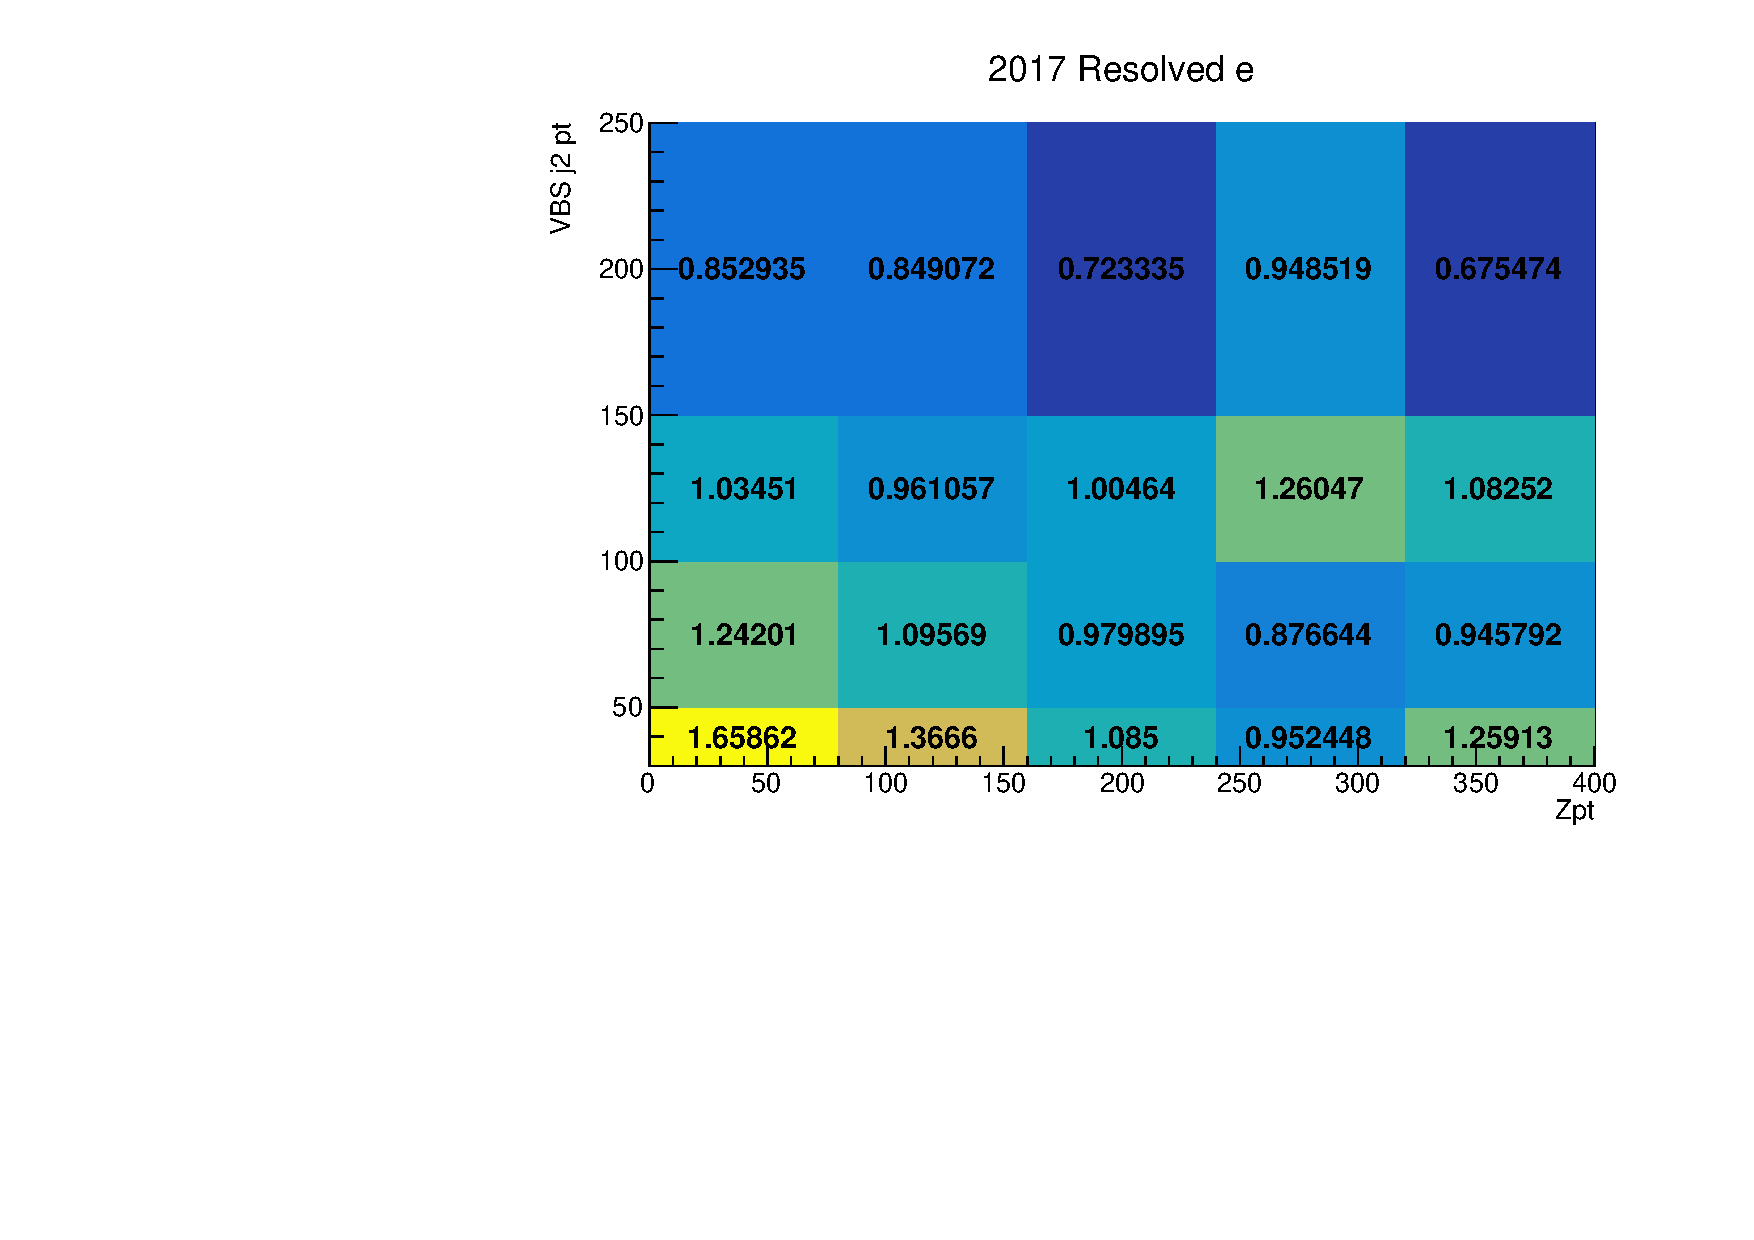
\includegraphics[width=0.45\textwidth]{analysis_plots/dyjet_norm_2d/cr_vjets_e_sf_from_2017_zjj.pdf}
  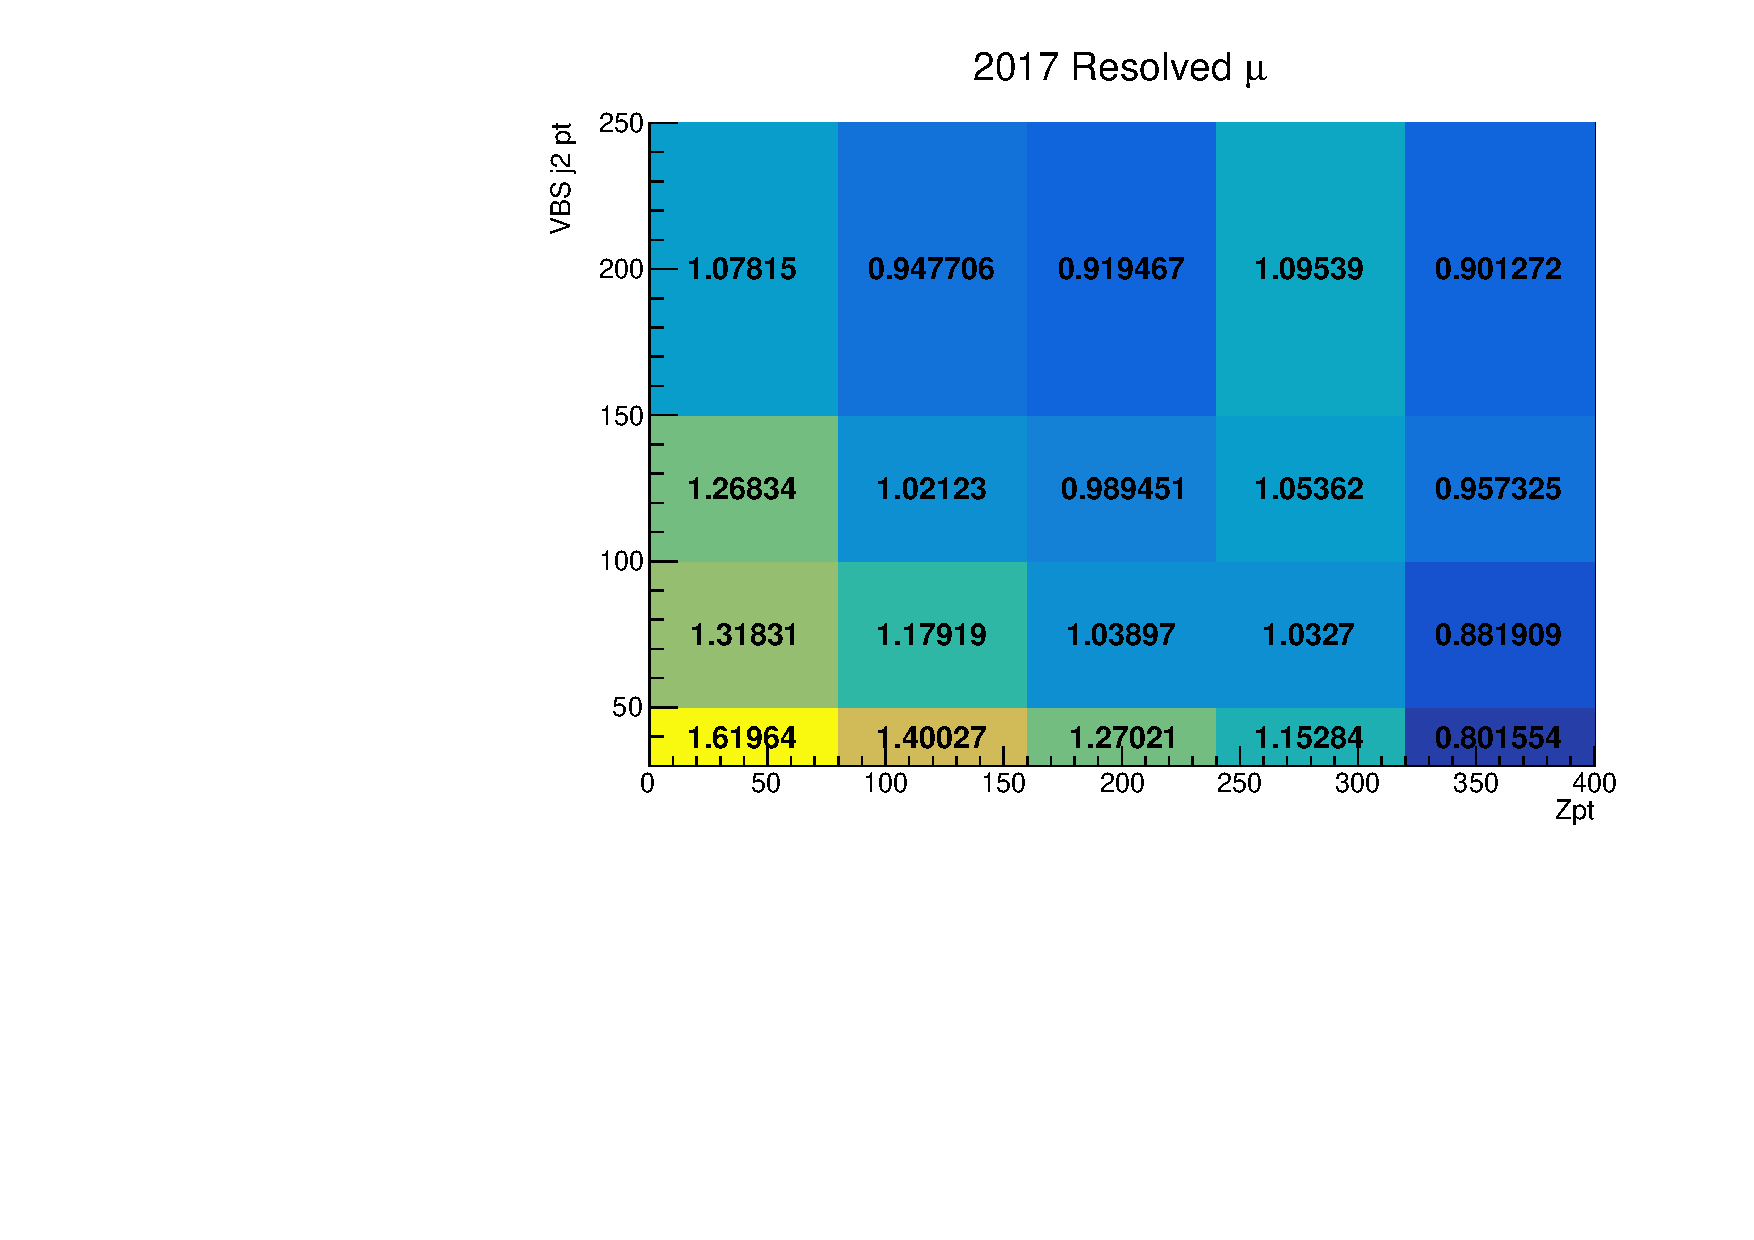
\includegraphics[width=0.45\textwidth]{analysis_plots/dyjet_norm_2d/cr_vjets_mu_sf_from_2017_zjj.pdf}\\
  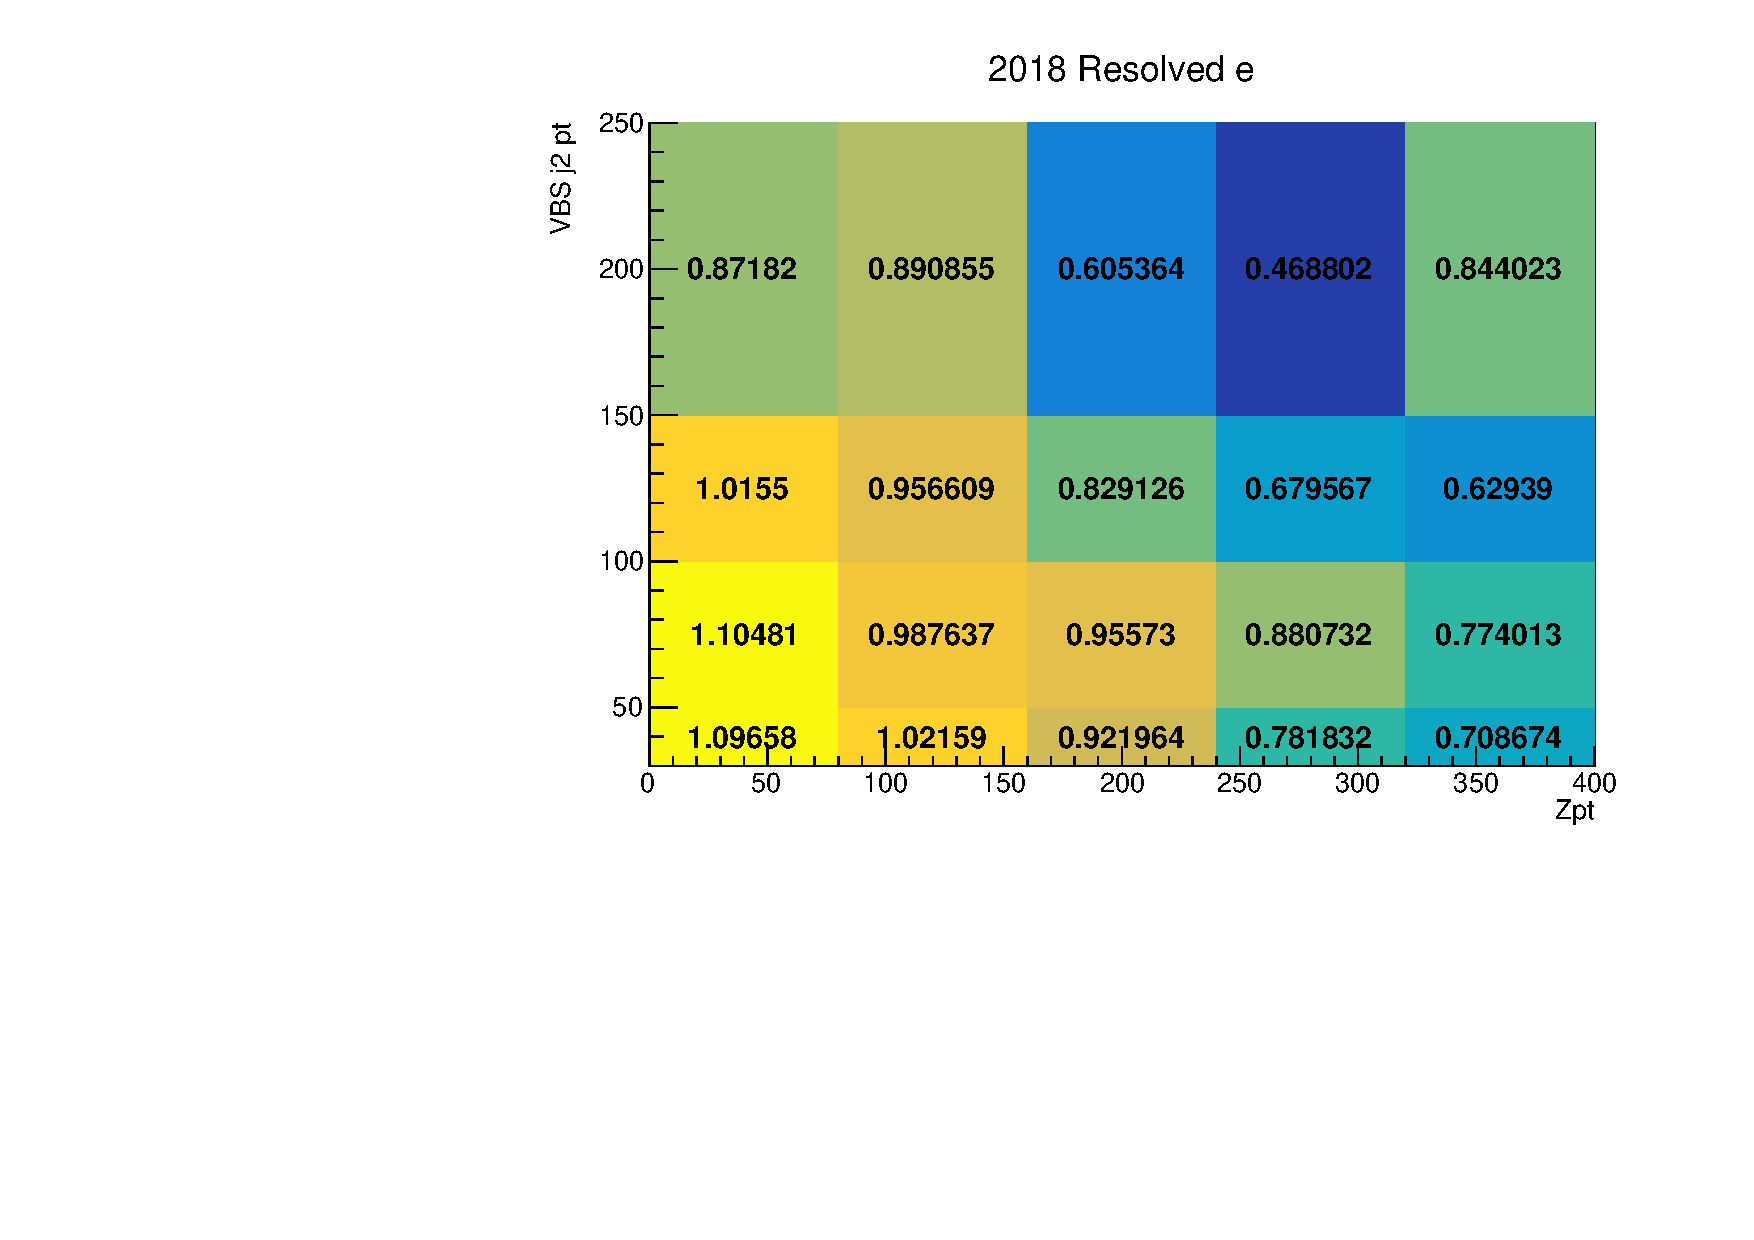
\includegraphics[width=0.45\textwidth]{analysis_plots/dyjet_norm_2d/cr_vjets_e_sf_from_2018_zjj.pdf}
  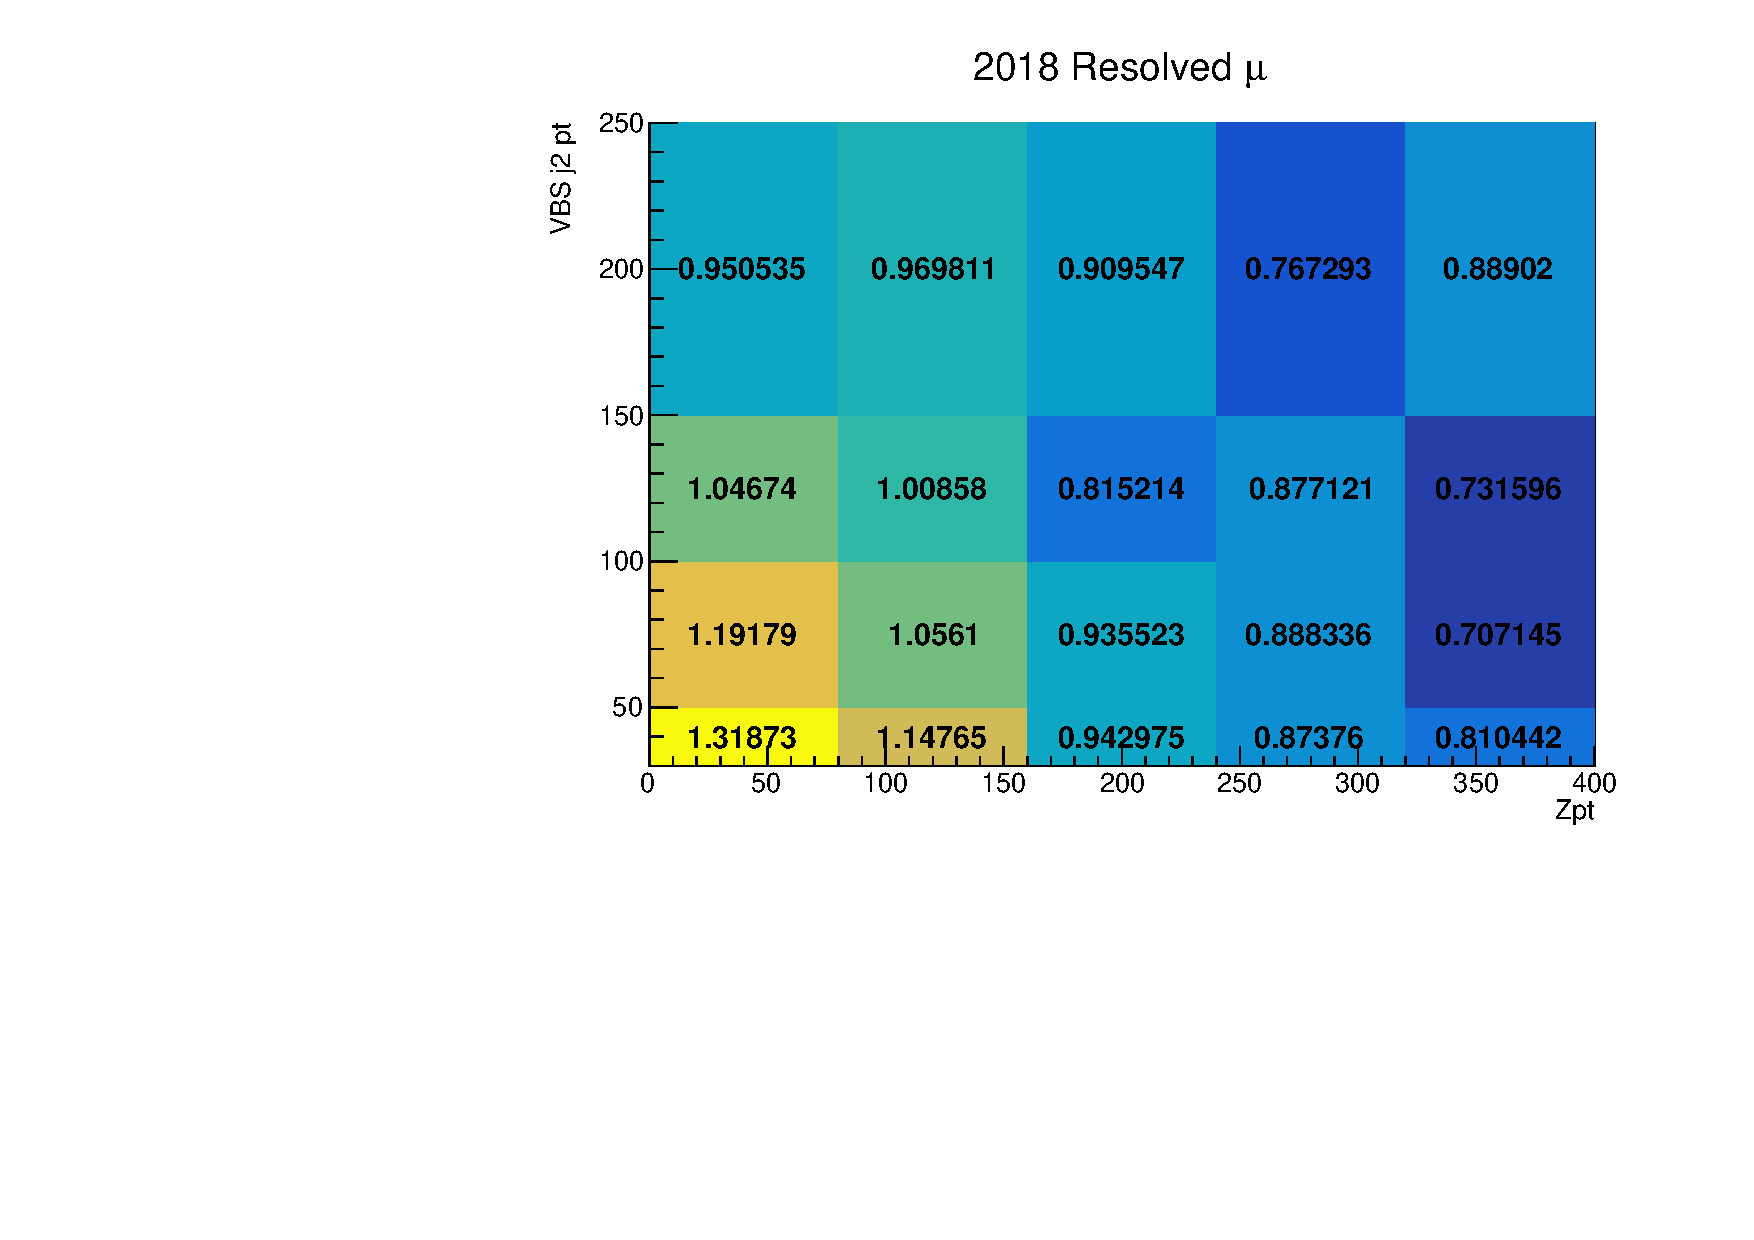
\includegraphics[width=0.45\textwidth]{analysis_plots/dyjet_norm_2d/cr_vjets_mu_sf_from_2018_zjj.pdf}
  \caption[Normalization factors from 1D bin of \( p_T \) of \textit{Z}
    and VBS trailing jet]%
  {Normalization factors from 1D bin of \( p_T \) of \textit{Z}
    and VBS trailing jet. Top to Bottom: 2017 and 2018 resolved.
    Left to Right: electron and muon channel.}%
  \label{fig:norm-factors-2d}
\end{figure}


\clearpage
\section{Kinematics Distributions}

To understand how the kinematics of various final state objects and
the candidate constructed from them behave, they are studied in the control
region by stacking up all the background histograms and
overlaying them with the data as points.
Signal \gls{MC} is also overlayed on the histograms, since it's small,
for visualization purposes it's scaled with a factor shown in
the legends of the plots.

The kinematics plots also include a ratio plot of data and total background
\gls{MC}, and uncertainties in histograms of \gls{MC} are shown as shaded region
which includes total statistical bin error, total \gls{JES} and
theoretical renormalization (QCD scale) error on the DY+Jets and VBS\_QCD \gls{MC} samples.

Section~\ref{ch_vbs:boosted-plots} and~\ref{ch_vbs:resolved-plots}
shows kinematics plots in control region for boosted and
resolved \textit{ZV} category respectively. These distributions show reasonable
agreement of data-to-\gls{MC} within statistical fluctuations.
This shows that our background is well modeled in control region.

\clearpage{}
\subsection{
  Boosted ZV DY+Jets Control Region
}\label{ch_vbs:boosted-plots}

\begin{figure}[!ht]
  \centering
  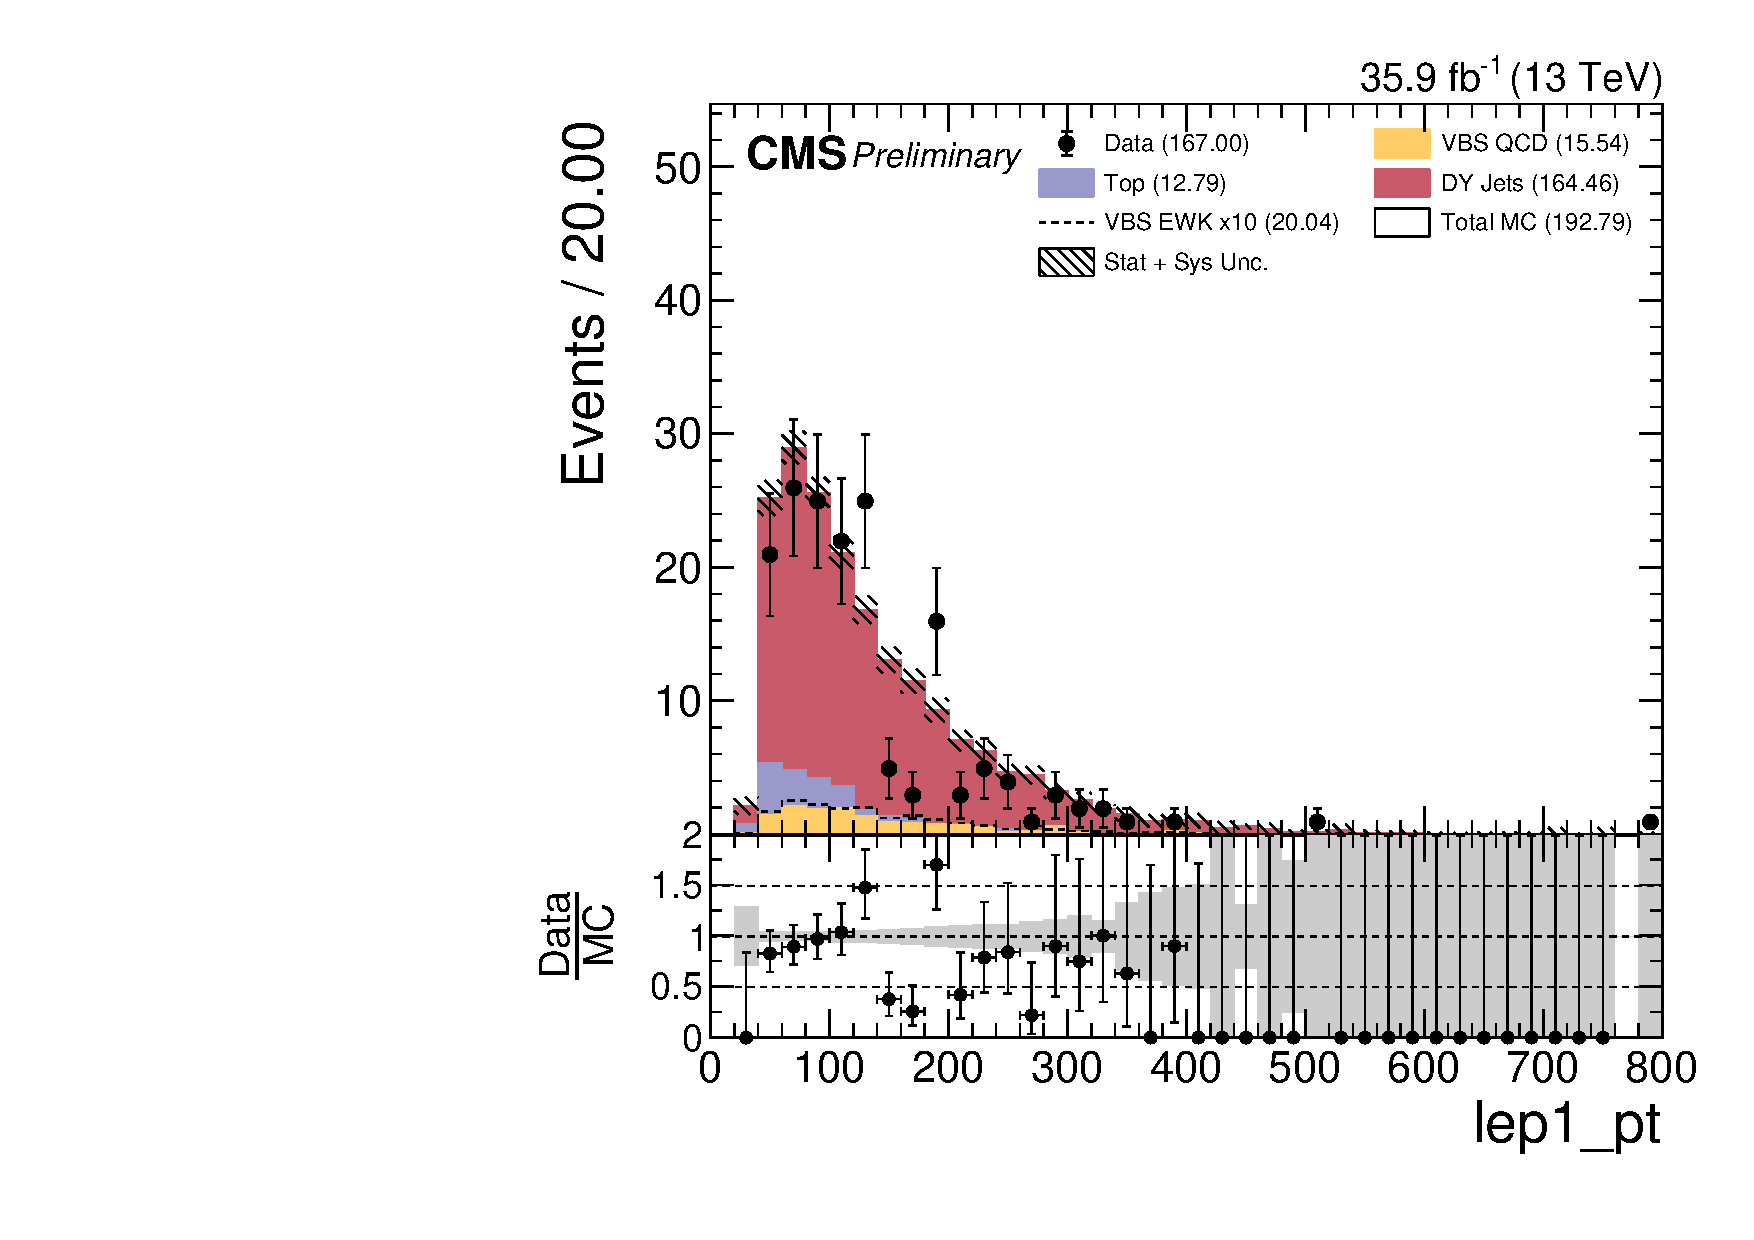
\includegraphics[width=0.335\textwidth]{analysis_plots/2016_zv/cr_vjets_e/lep1_pt.pdf} \hspace{-10pt}
  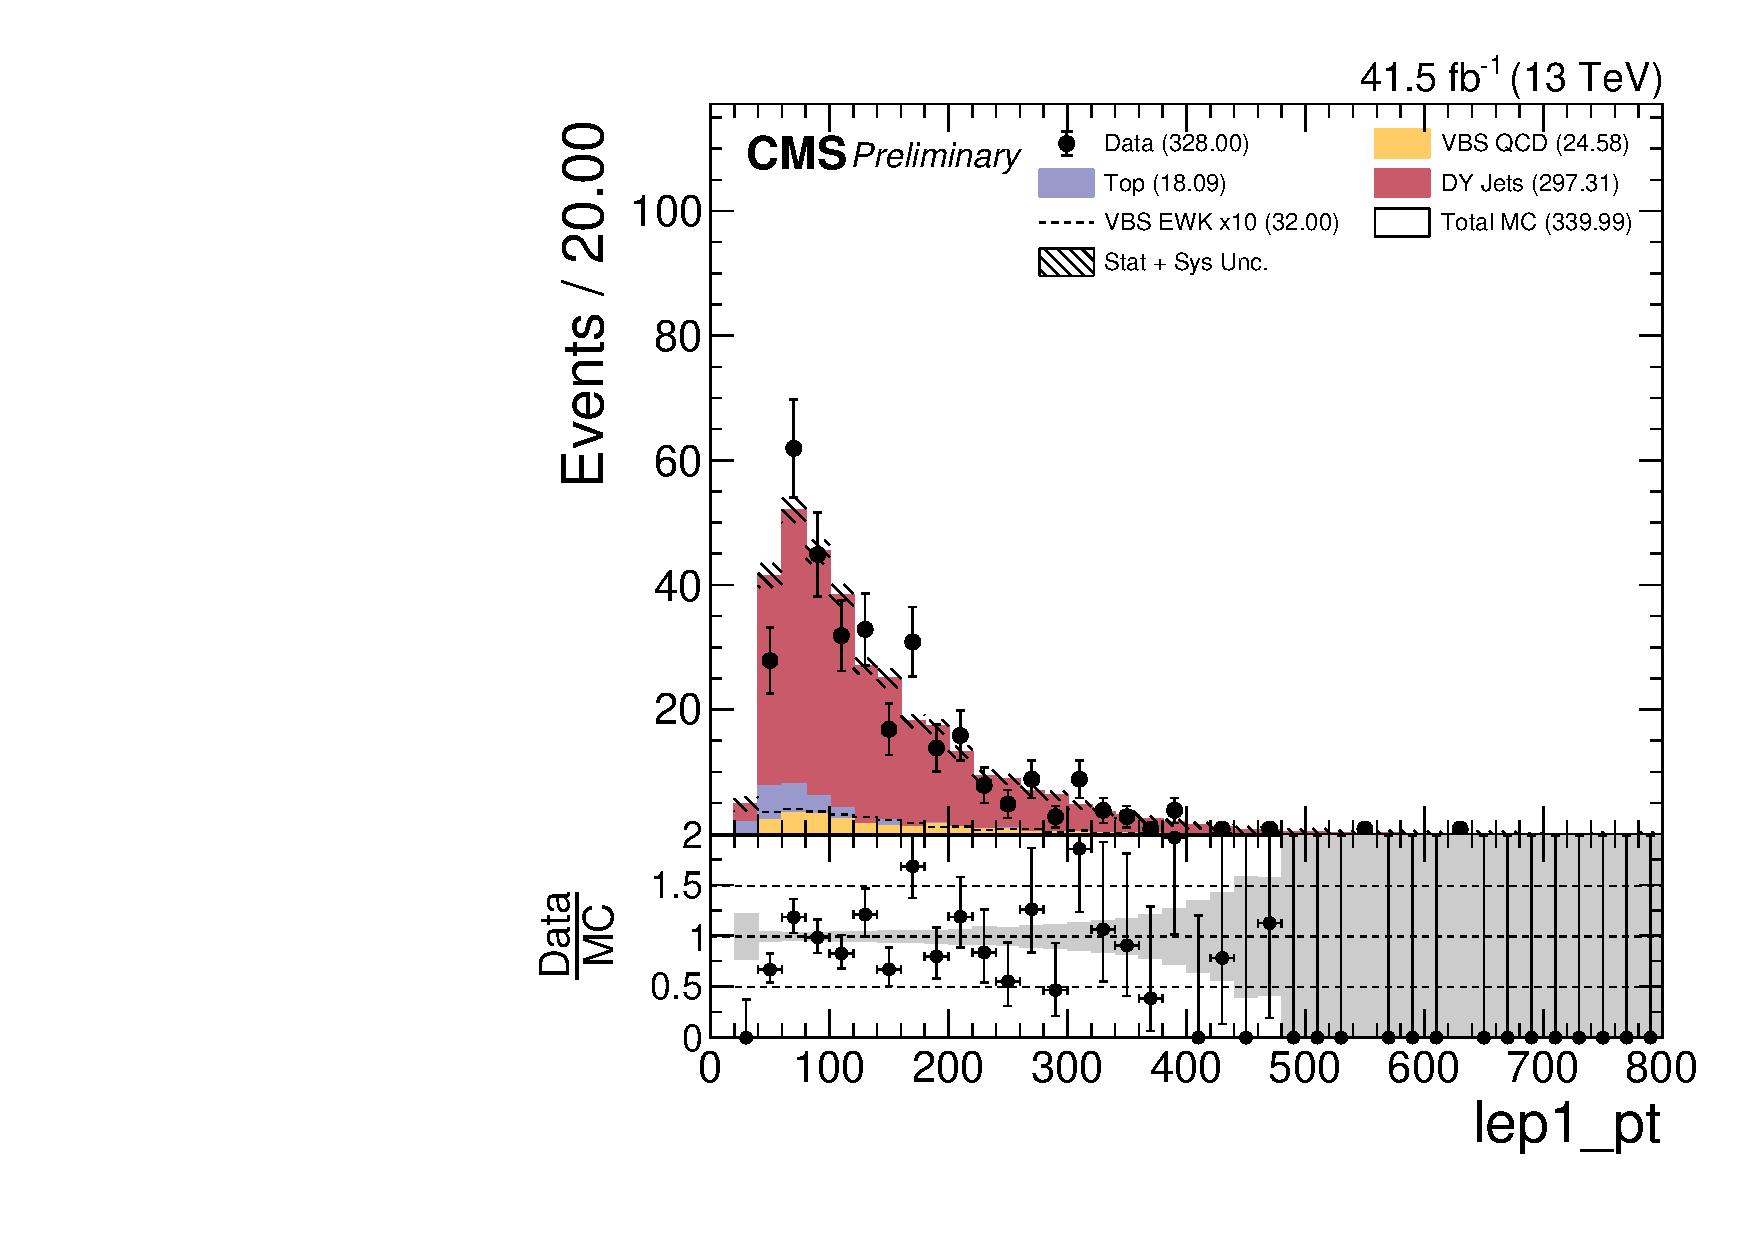
\includegraphics[width=0.335\textwidth]{analysis_plots/2017_zv/cr_vjets_e/lep1_pt.pdf} \hspace{-10pt}
  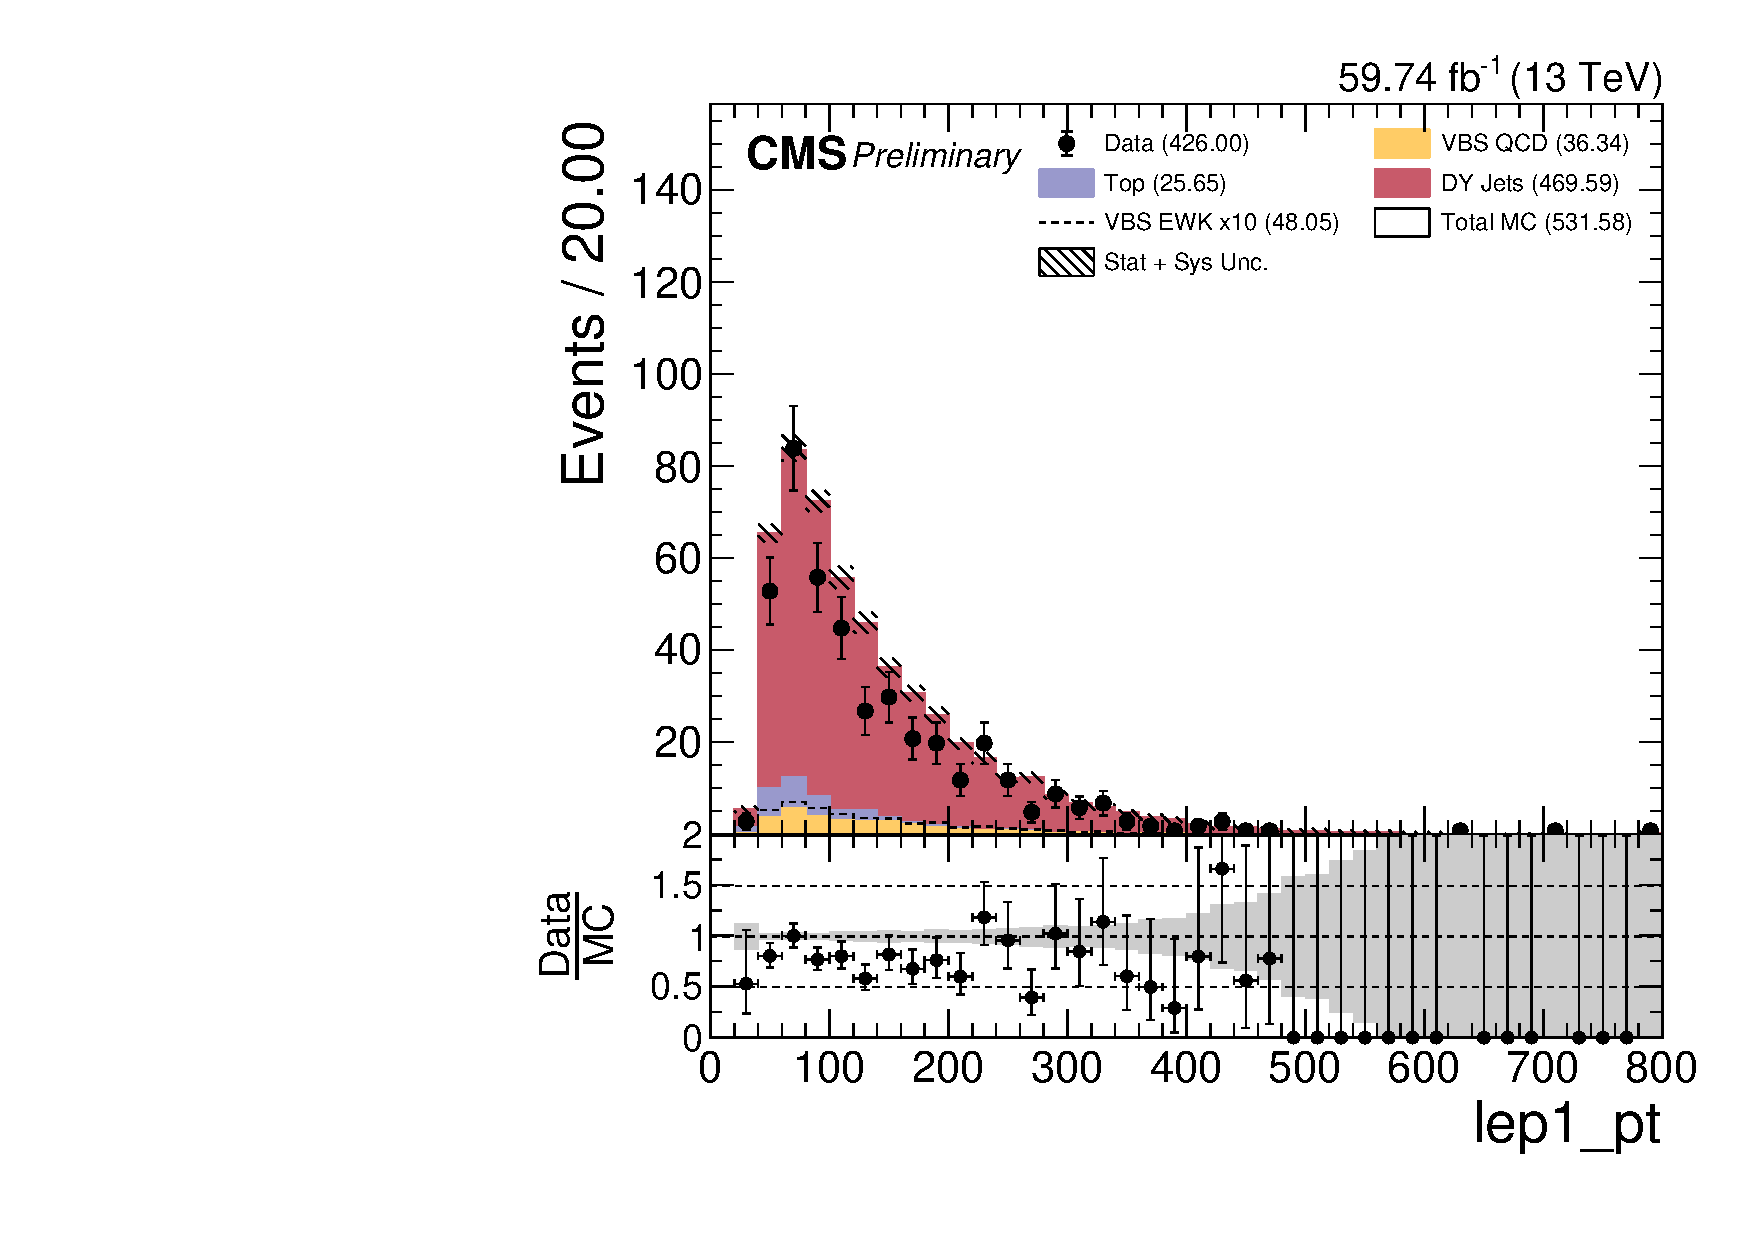
\includegraphics[width=0.335\textwidth]{analysis_plots/2018_zv/cr_vjets_e/lep1_pt.pdf} \hspace{-10pt} \\
  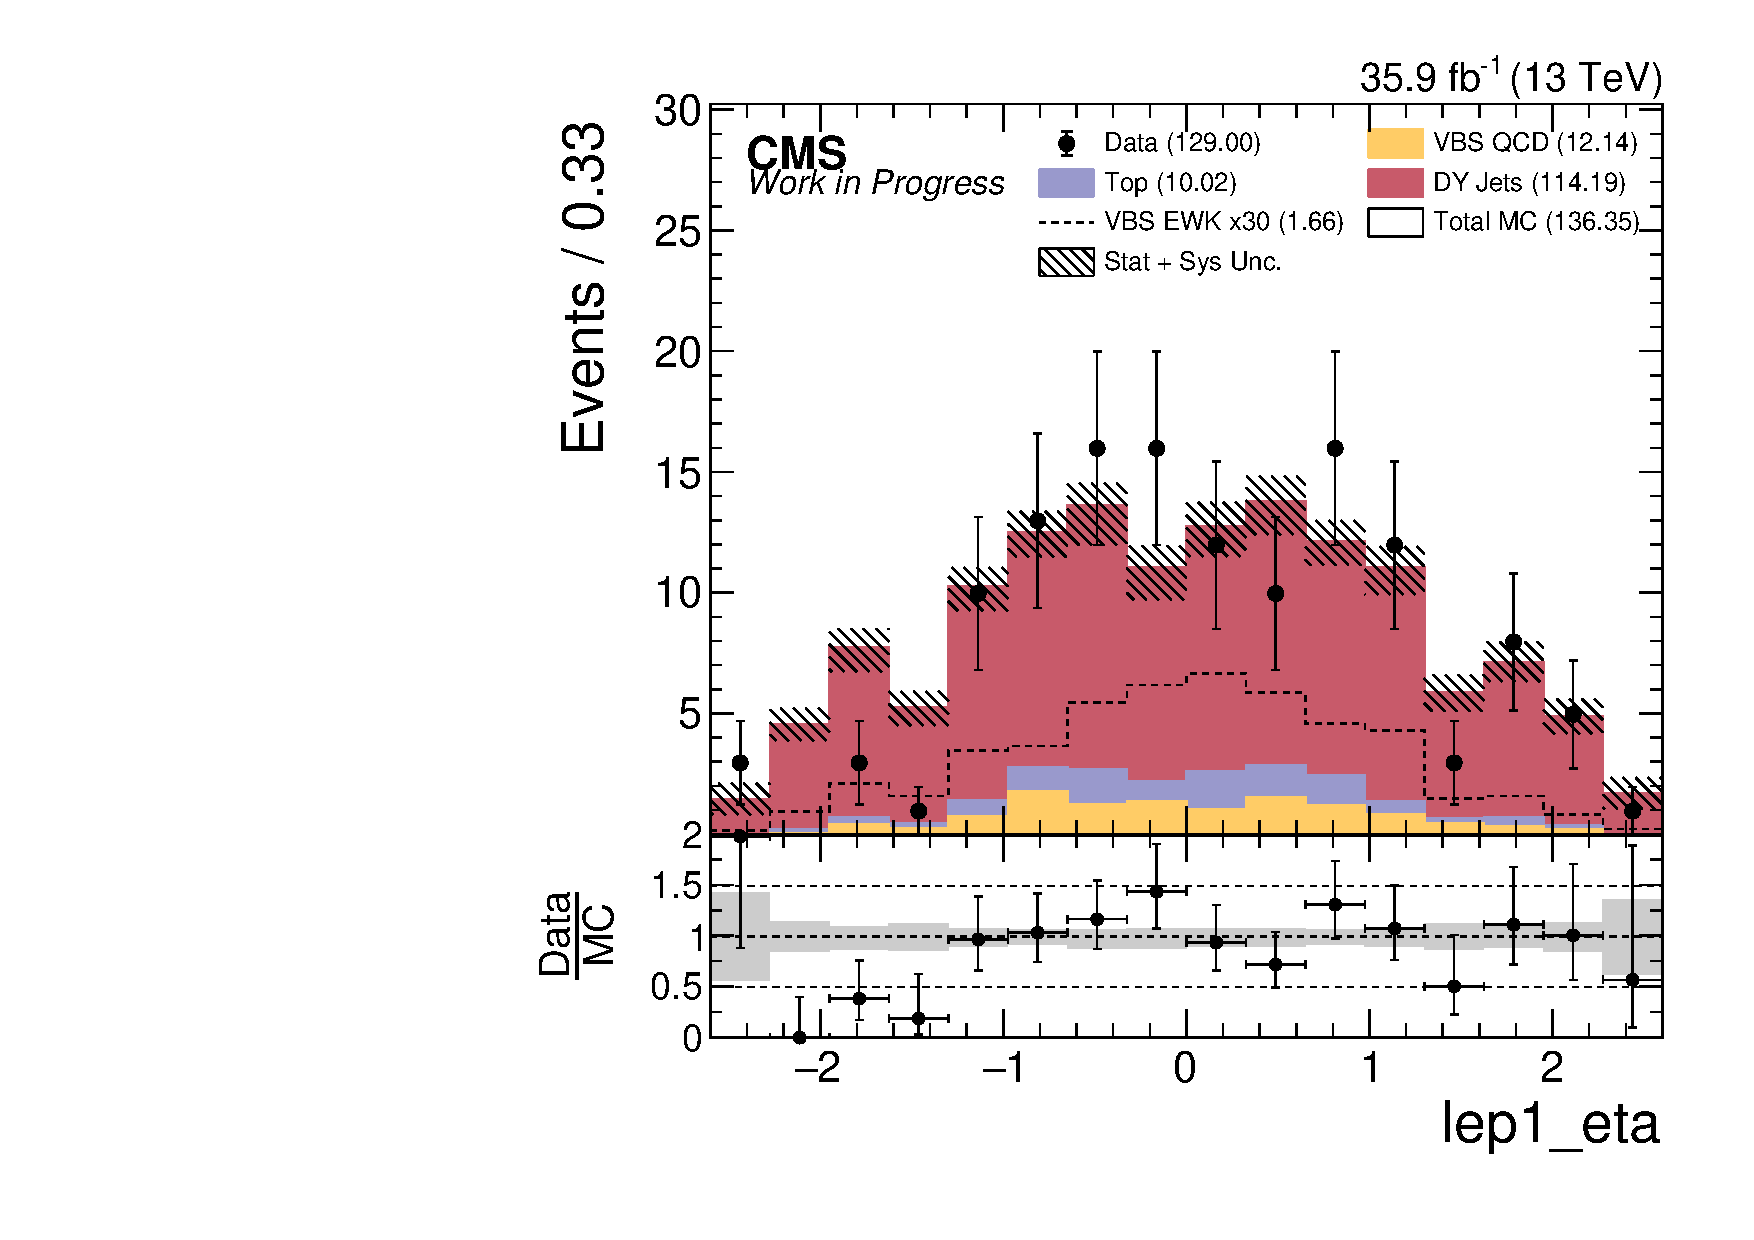
\includegraphics[width=0.335\textwidth]{analysis_plots/2016_zv/cr_vjets_e/lep1_eta.pdf} \hspace{-10pt}
  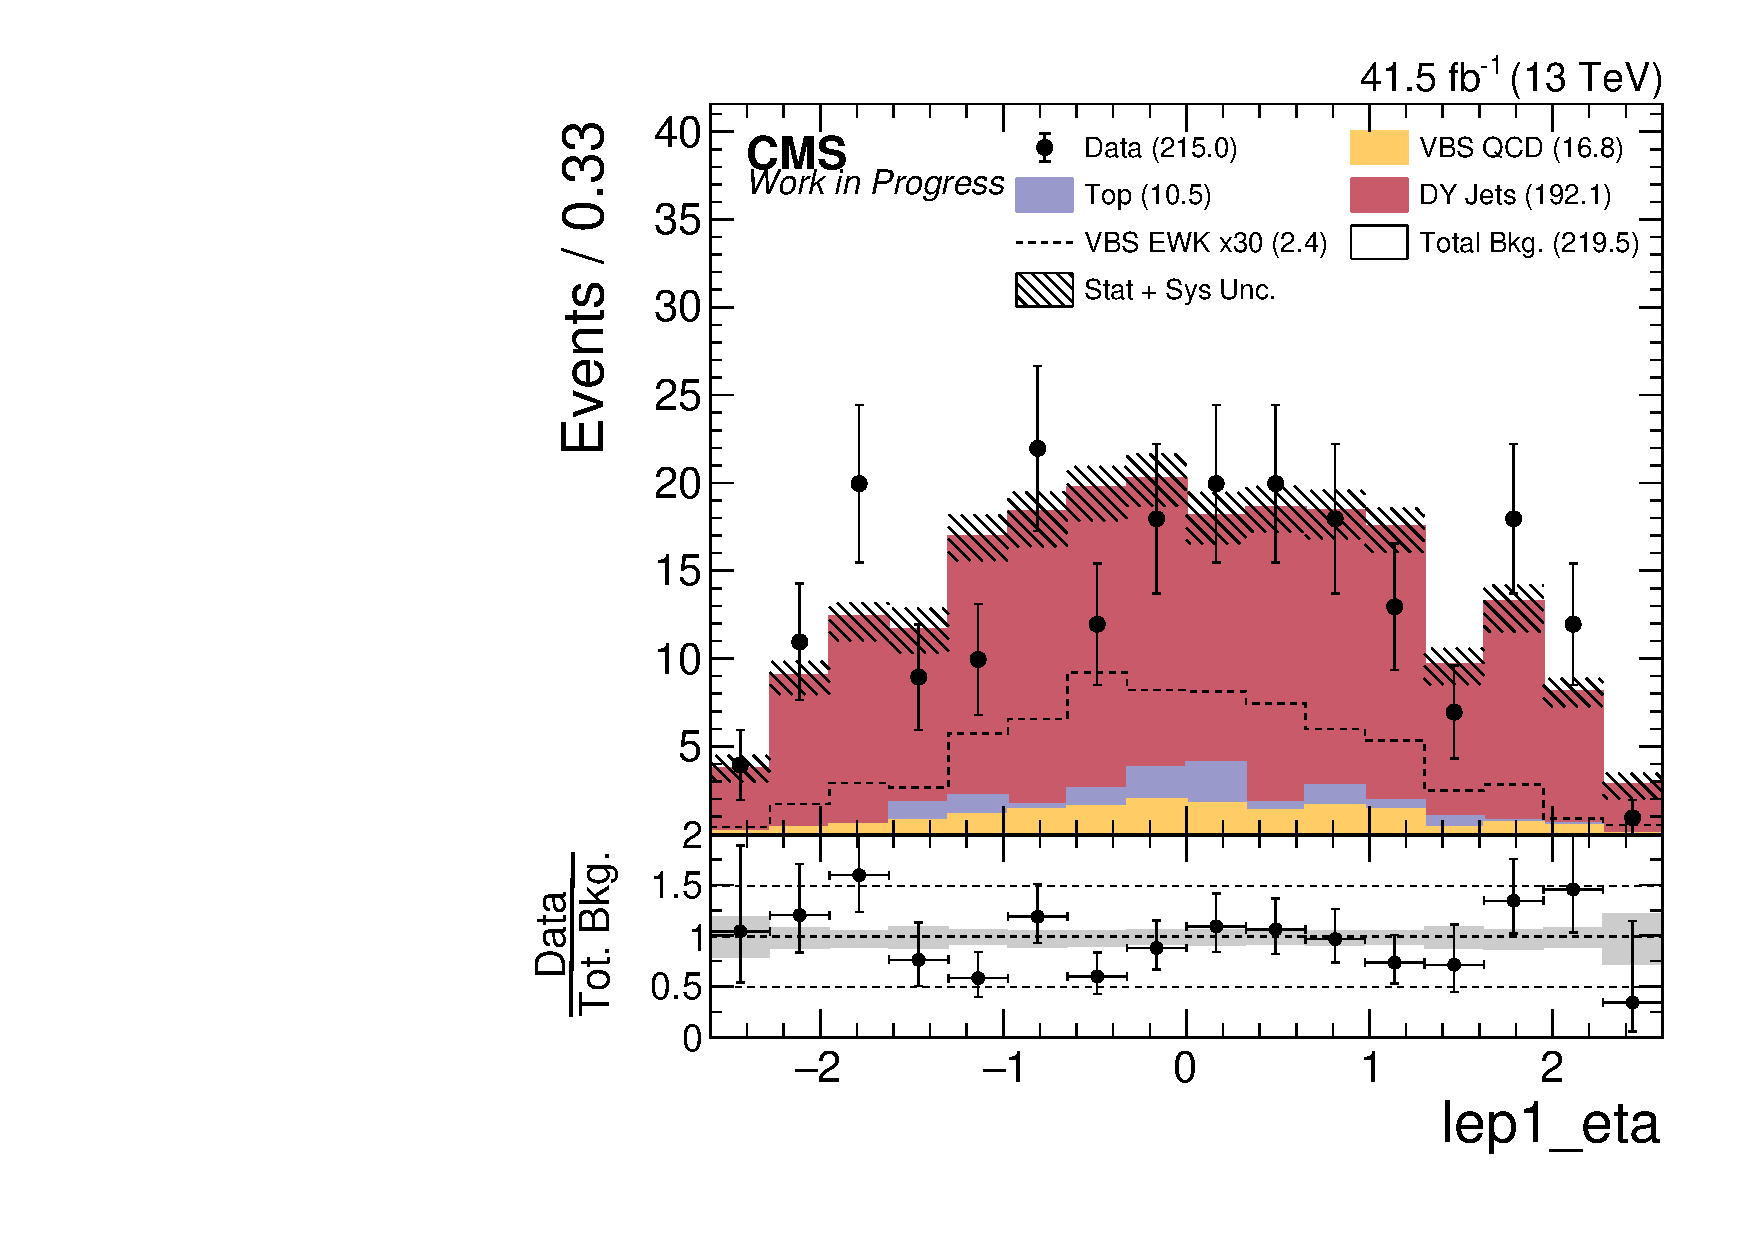
\includegraphics[width=0.335\textwidth]{analysis_plots/2017_zv/cr_vjets_e/lep1_eta.pdf} \hspace{-10pt}
  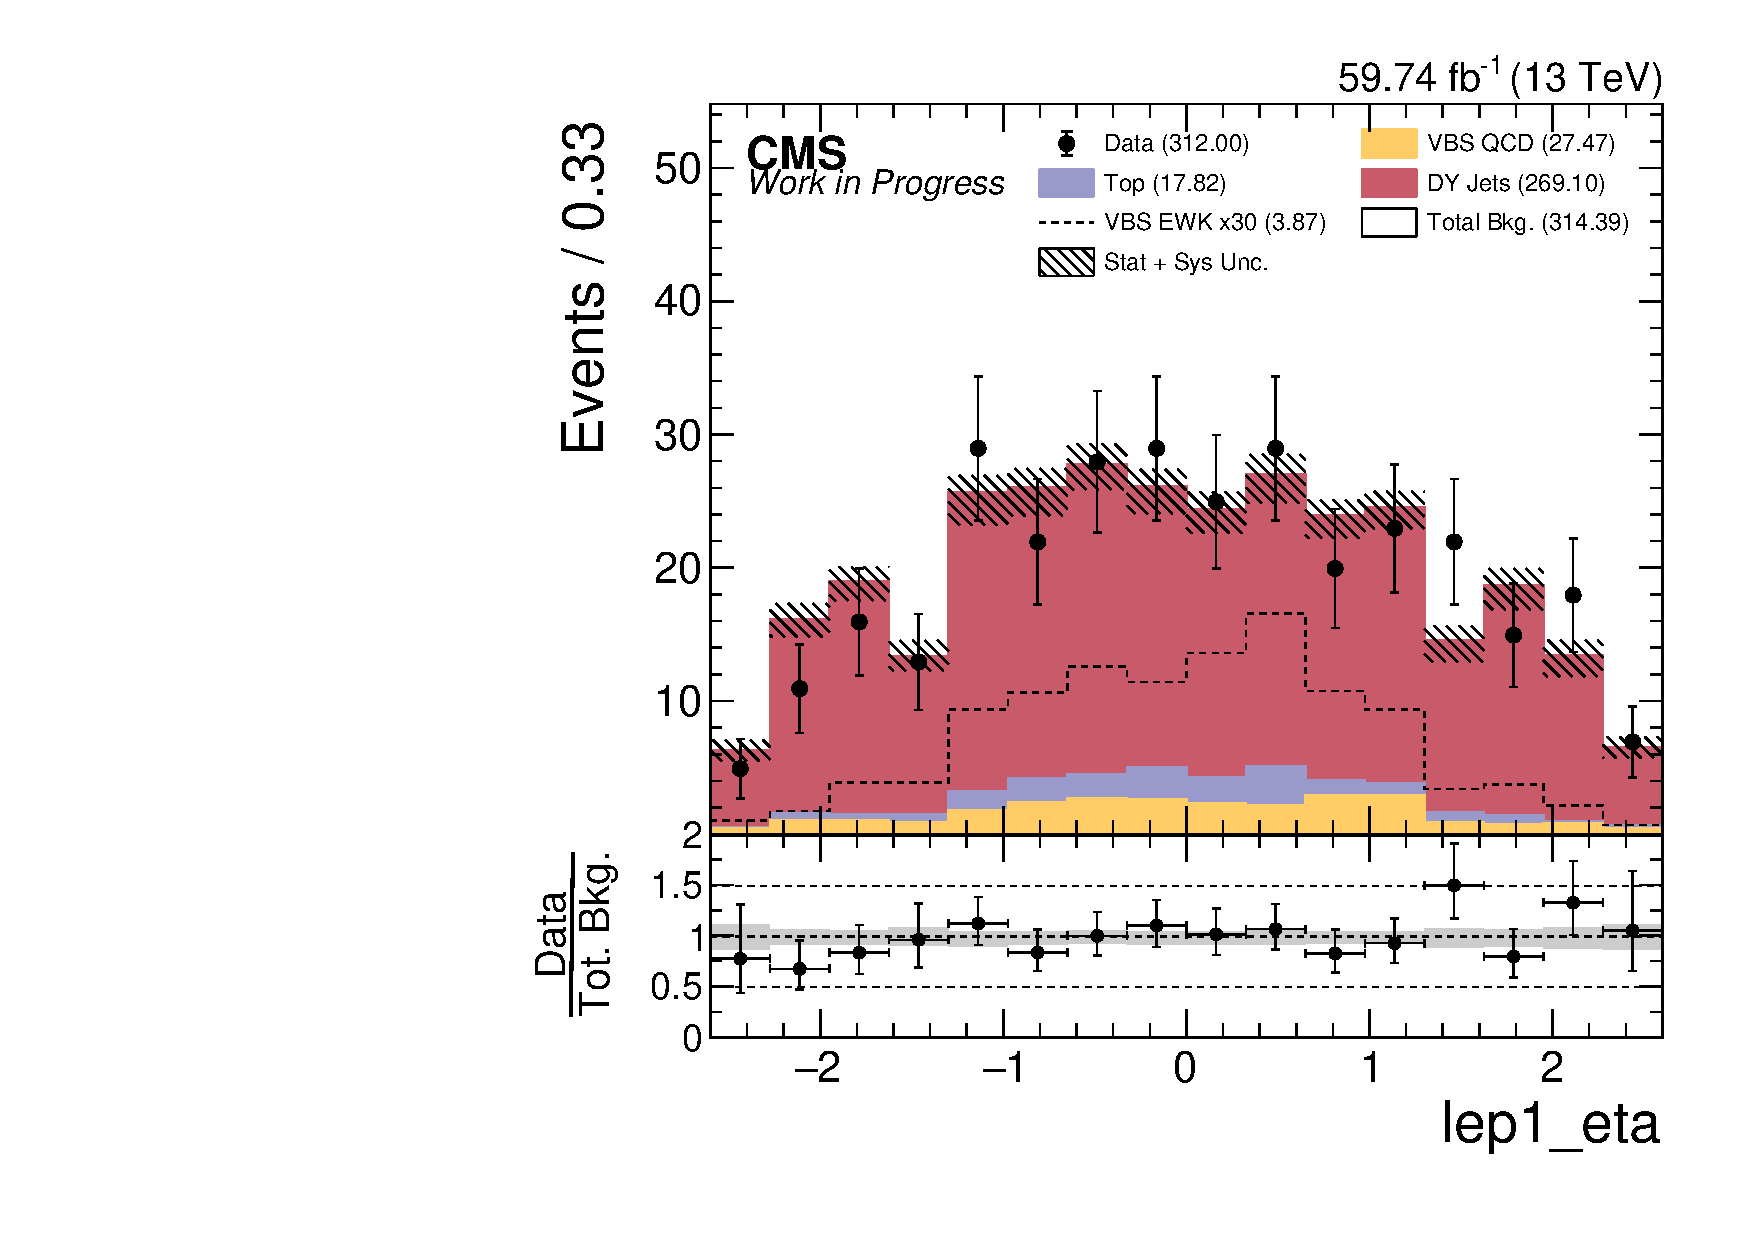
\includegraphics[width=0.335\textwidth]{analysis_plots/2018_zv/cr_vjets_e/lep1_eta.pdf} \hspace{-10pt} \\
  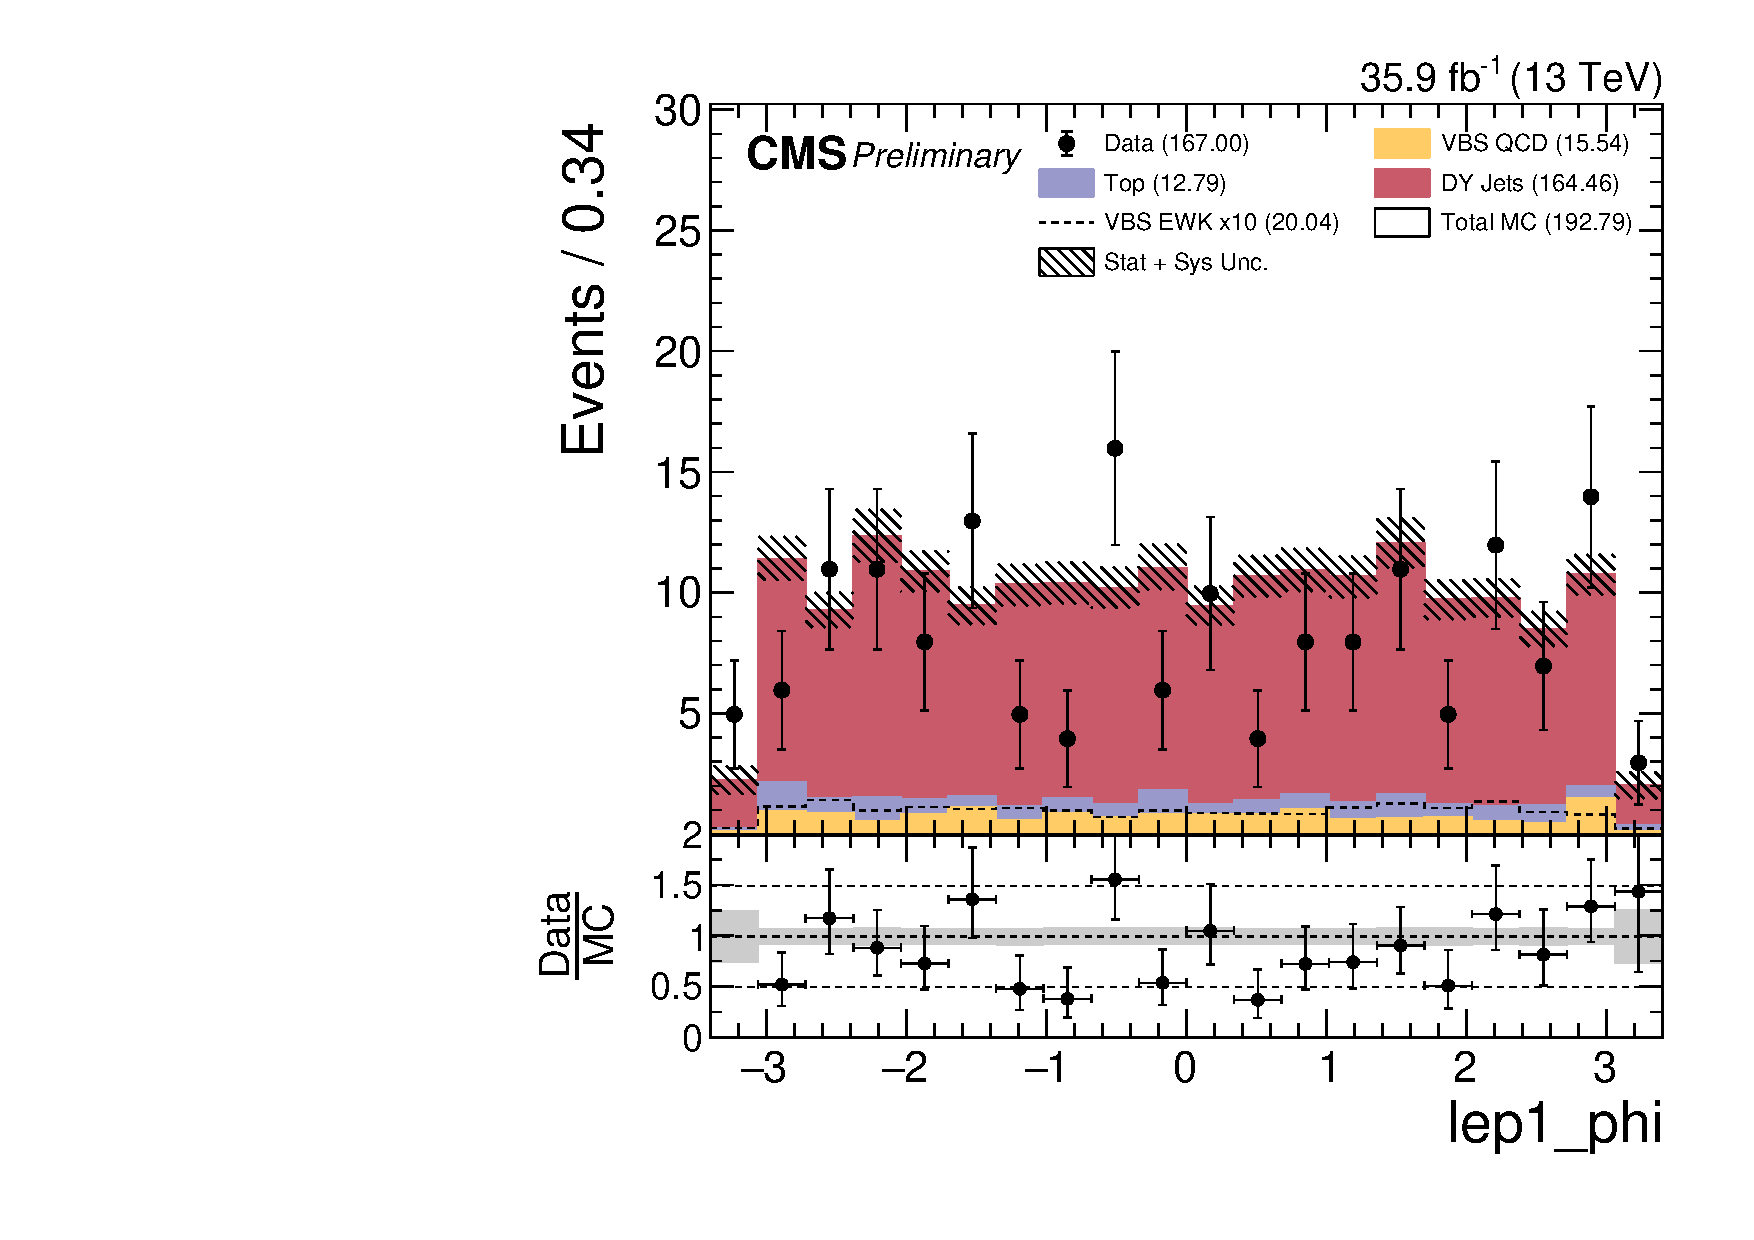
\includegraphics[width=0.335\textwidth]{analysis_plots/2016_zv/cr_vjets_e/lep1_phi.pdf} \hspace{-10pt}
  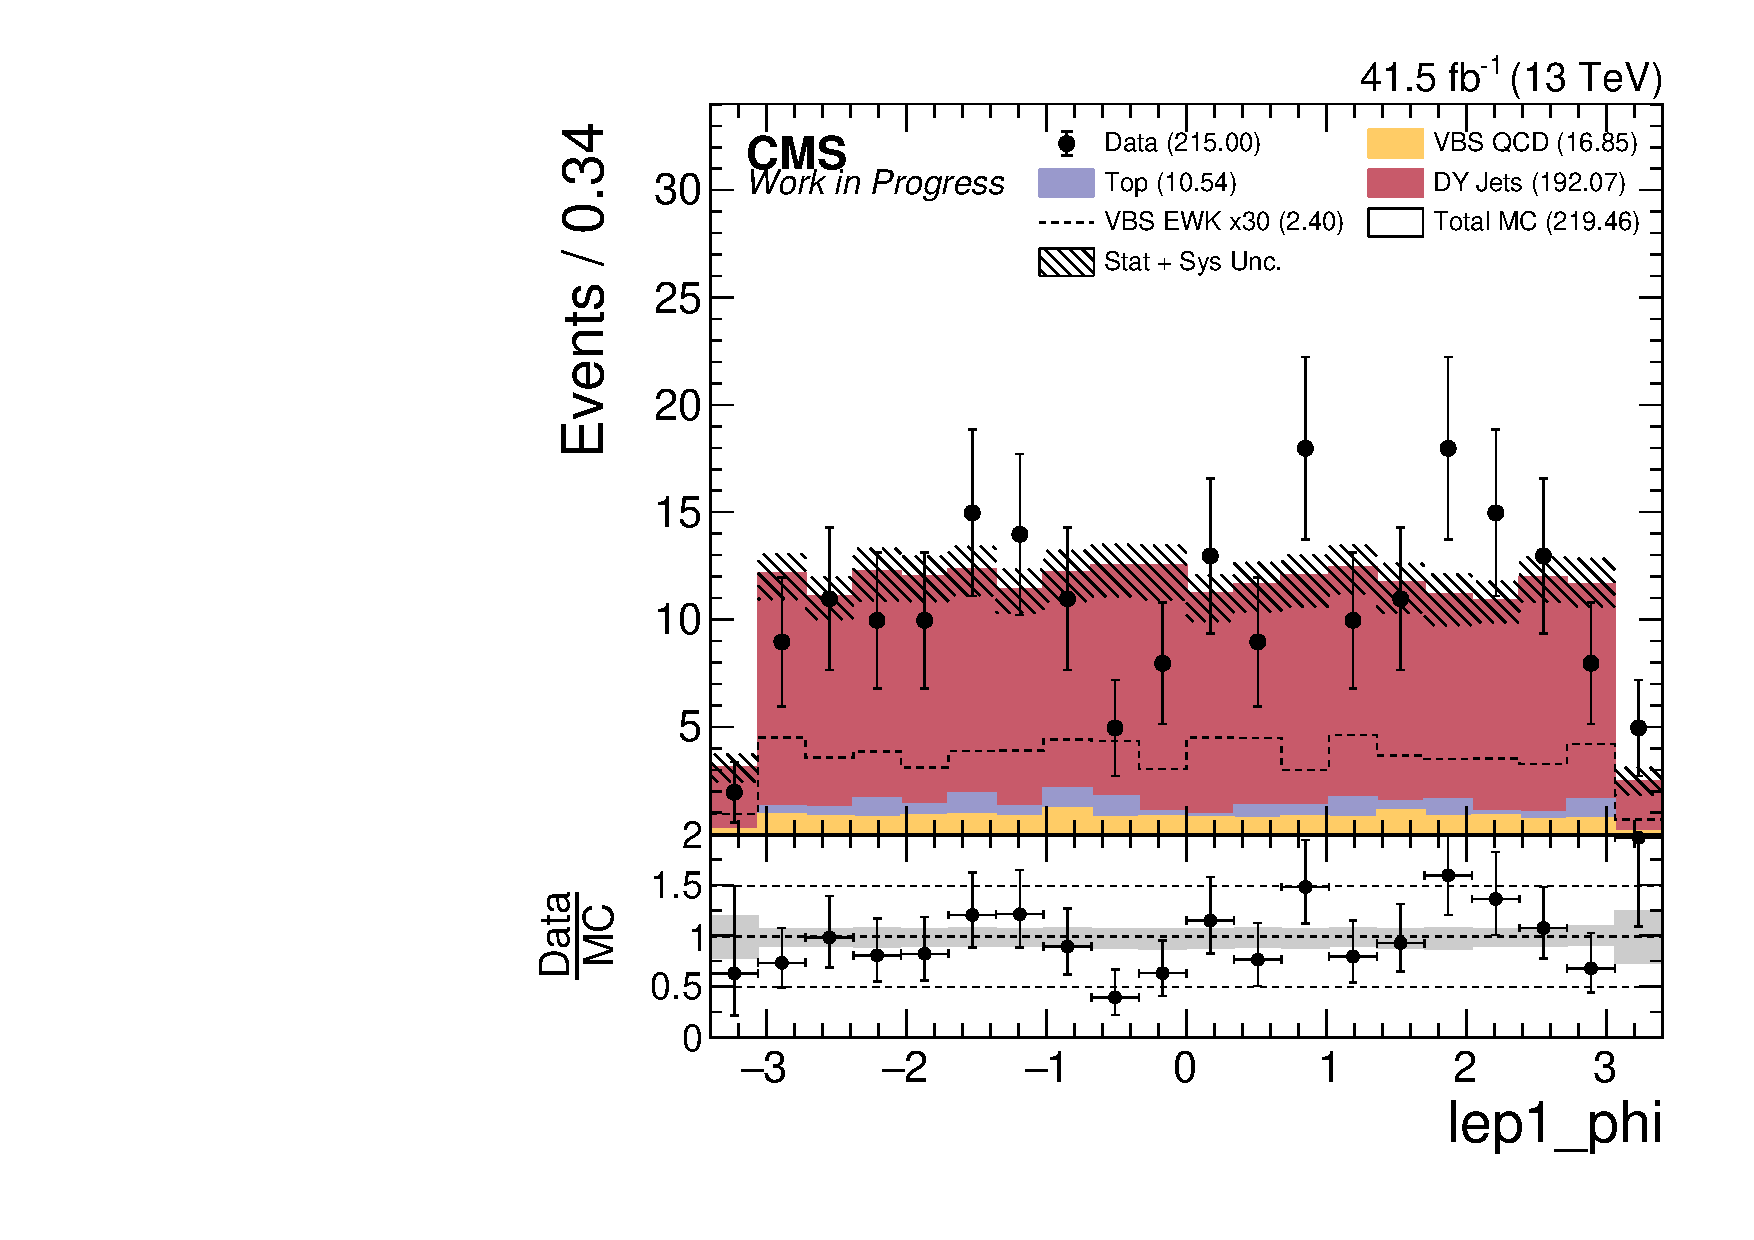
\includegraphics[width=0.335\textwidth]{analysis_plots/2017_zv/cr_vjets_e/lep1_phi.pdf} \hspace{-10pt}
  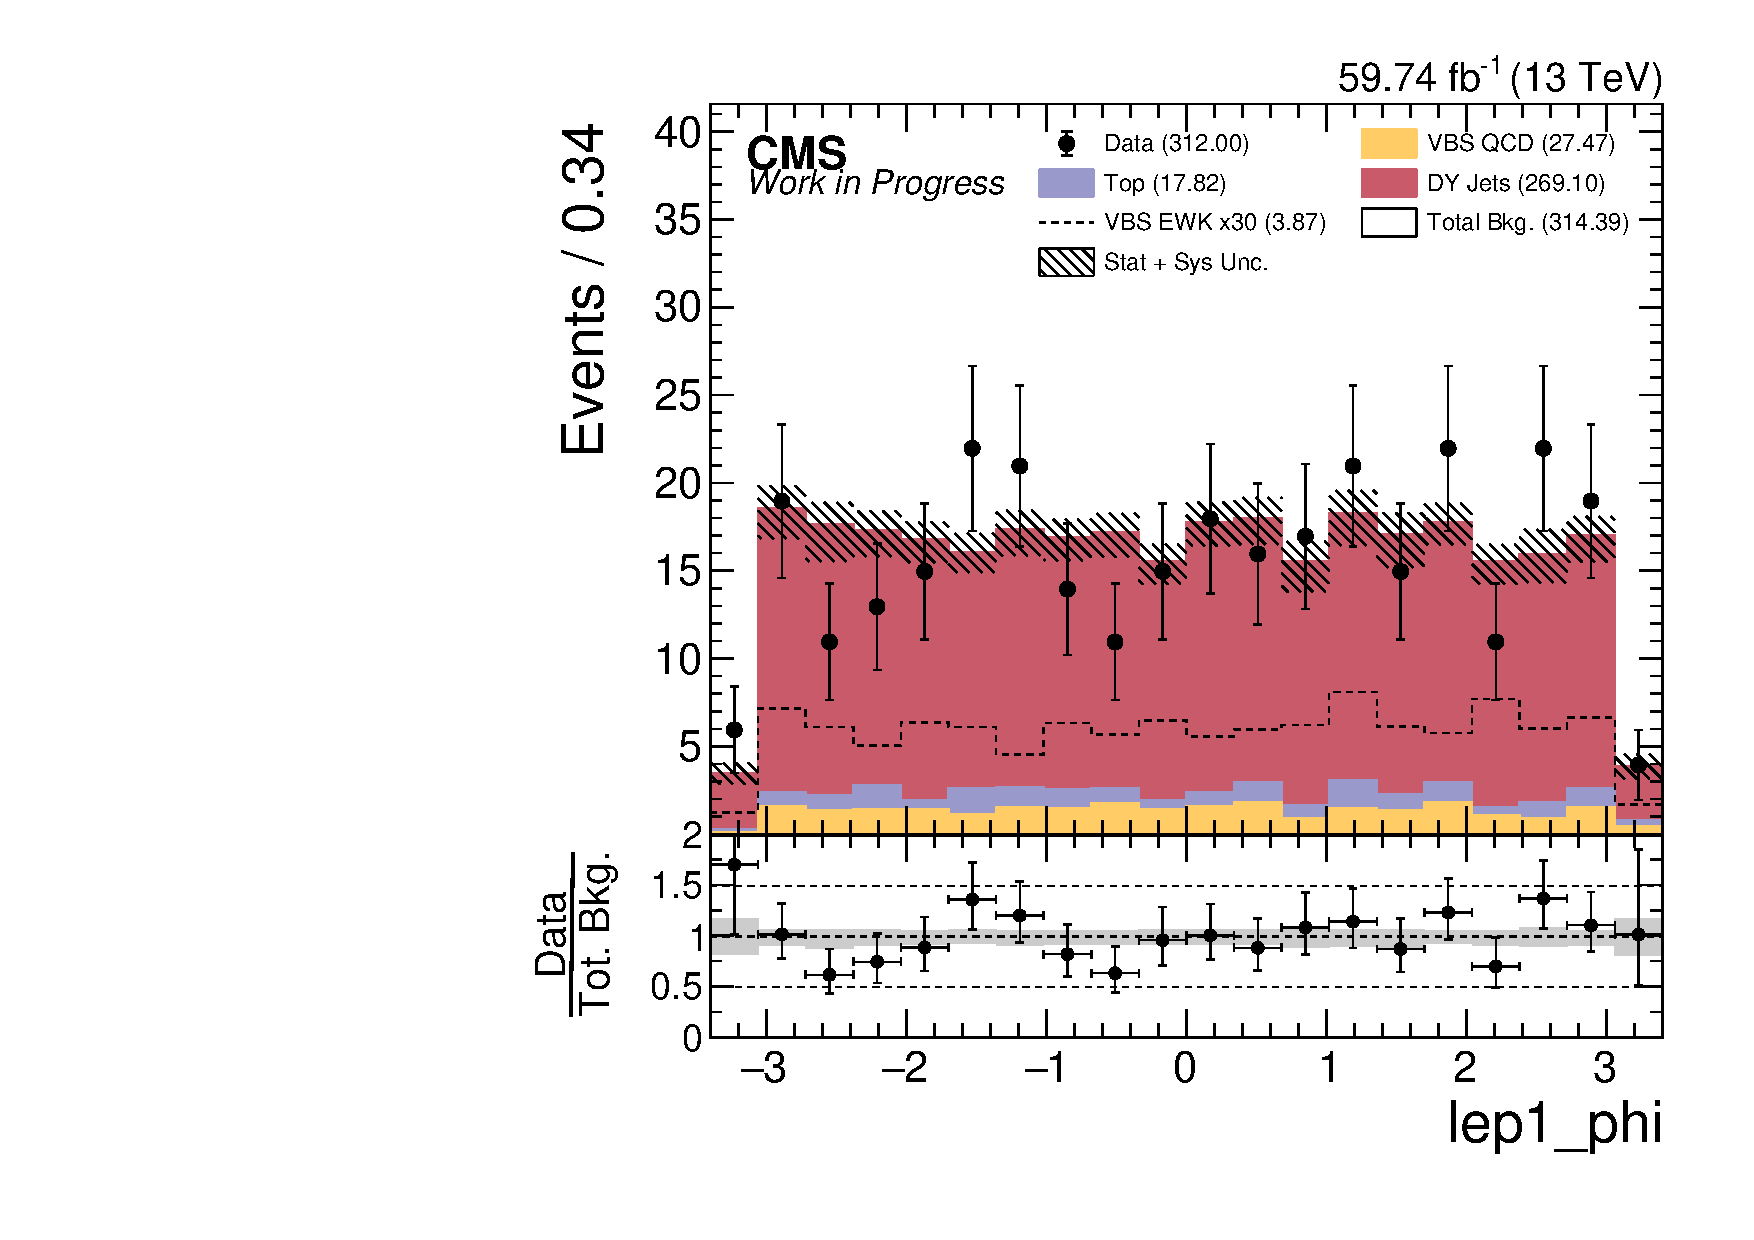
\includegraphics[width=0.335\textwidth]{analysis_plots/2018_zv/cr_vjets_e/lep1_phi.pdf} \hspace{-10pt} \\
  \caption[DY+Jets Control Region: Leading electron kinematics in Boosted ZV Channel]%
  {DY+Jets Control Region: Leading electron kinematics in Boosted ZV Channel.
    Error bars include statistical uncertainty on total background,
    JES and QCD scale systematic on DY+Jets and VBS\_QCD MC\@.
    From Left to Right: 2016,
    2017, and 2018. From Top to Bottom: \( p_T \), \( \eta \), and \( \phi \).}%
  \label{fig:zv-cr-vjets-e-lep1-pt-eta-phi}
\end{figure}

\begin{figure}[!ht]
  \centering
  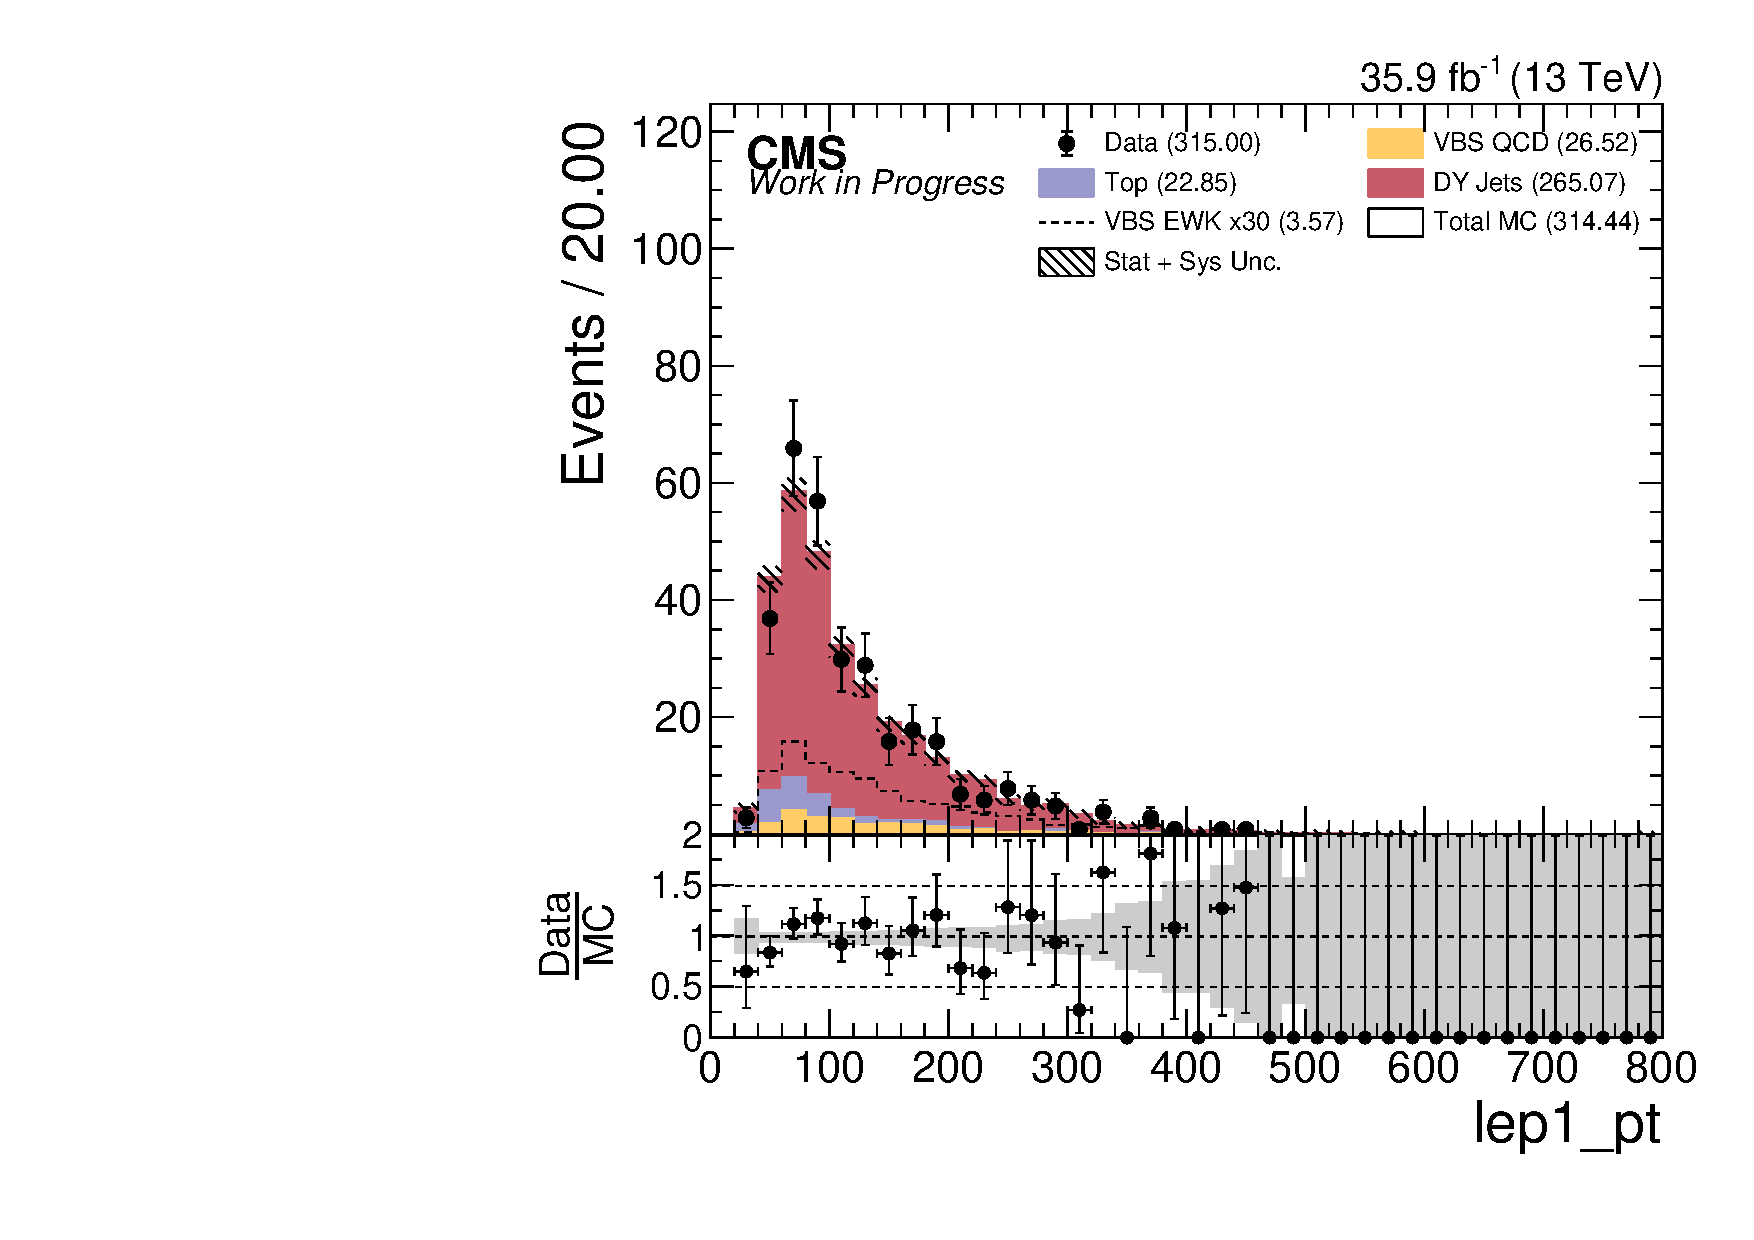
\includegraphics[width=0.335\textwidth]{analysis_plots/2016_zv/cr_vjets_m/lep1_pt.pdf} \hspace{-10pt}
  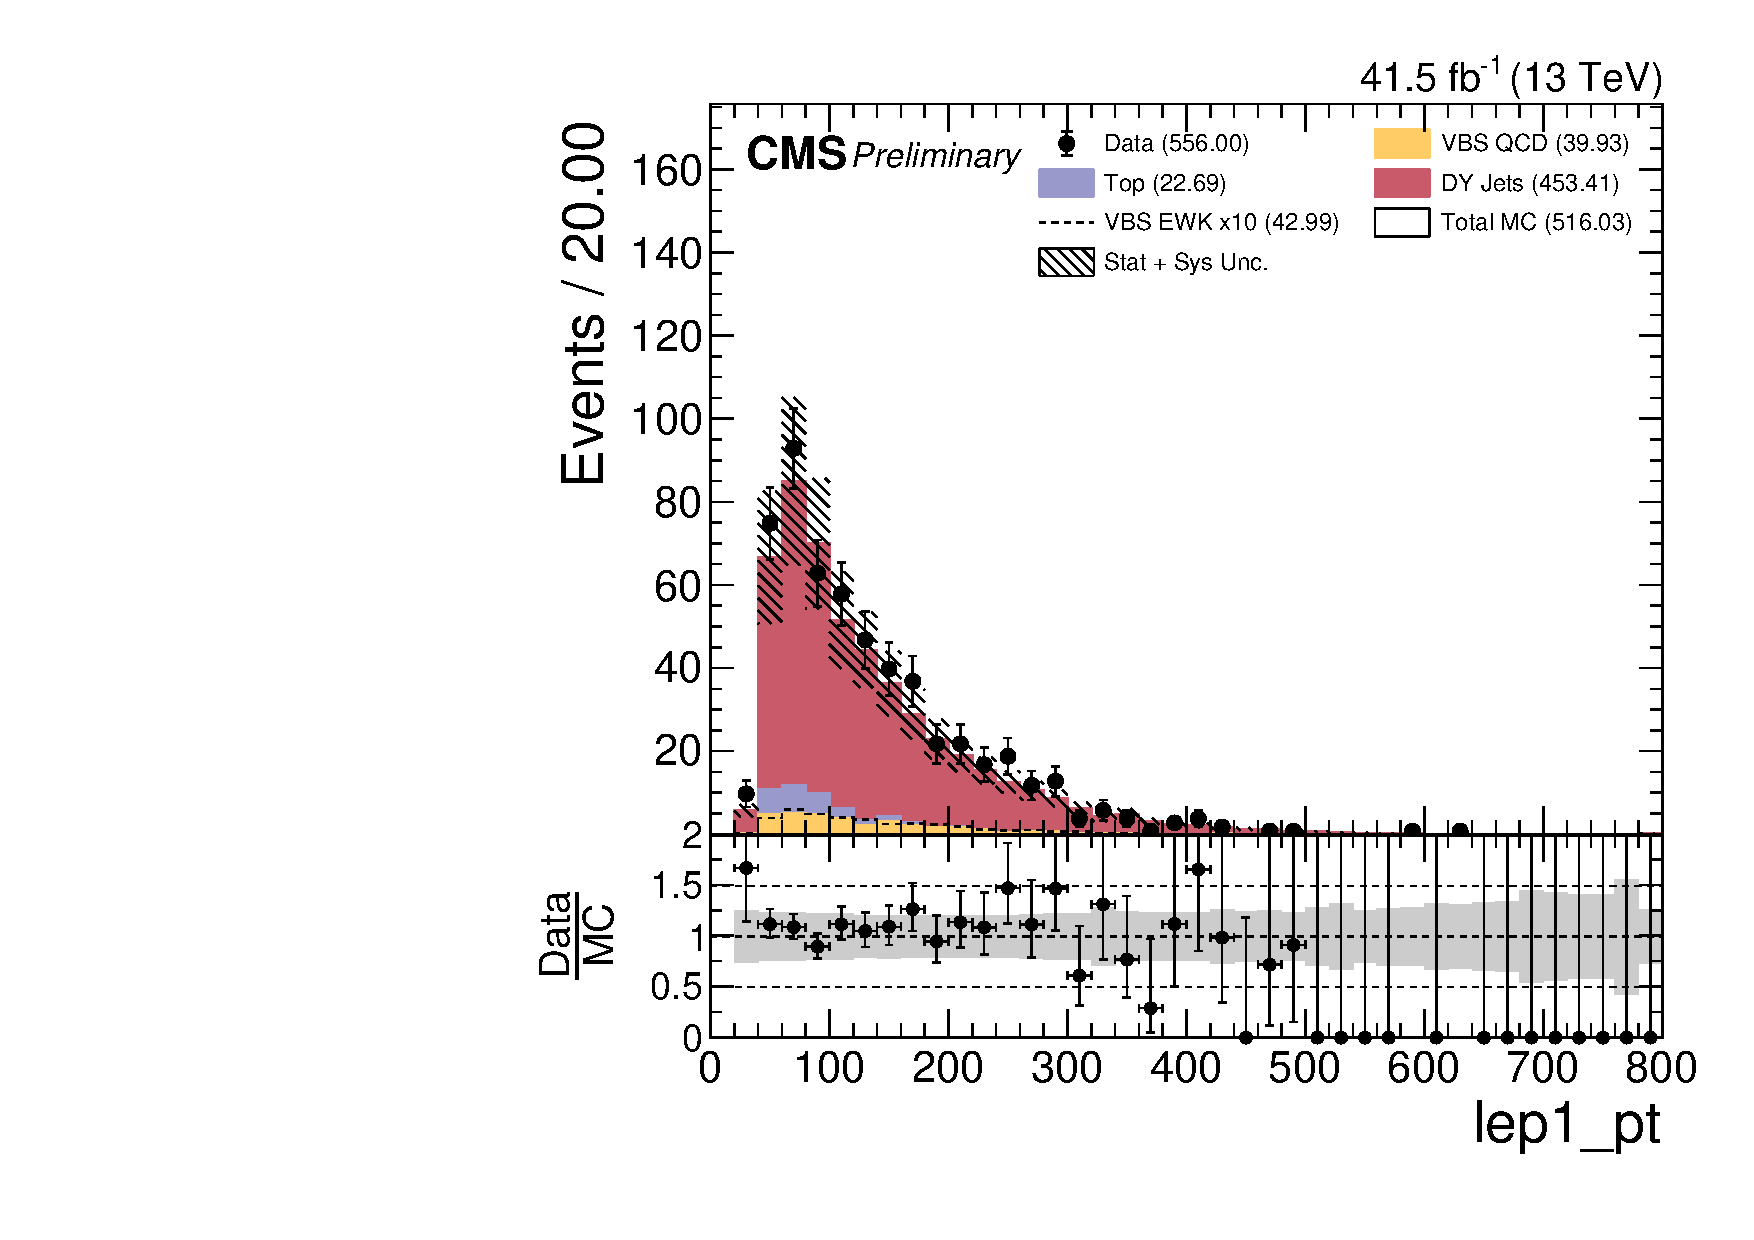
\includegraphics[width=0.335\textwidth]{analysis_plots/2017_zv/cr_vjets_m/lep1_pt.pdf} \hspace{-10pt}
  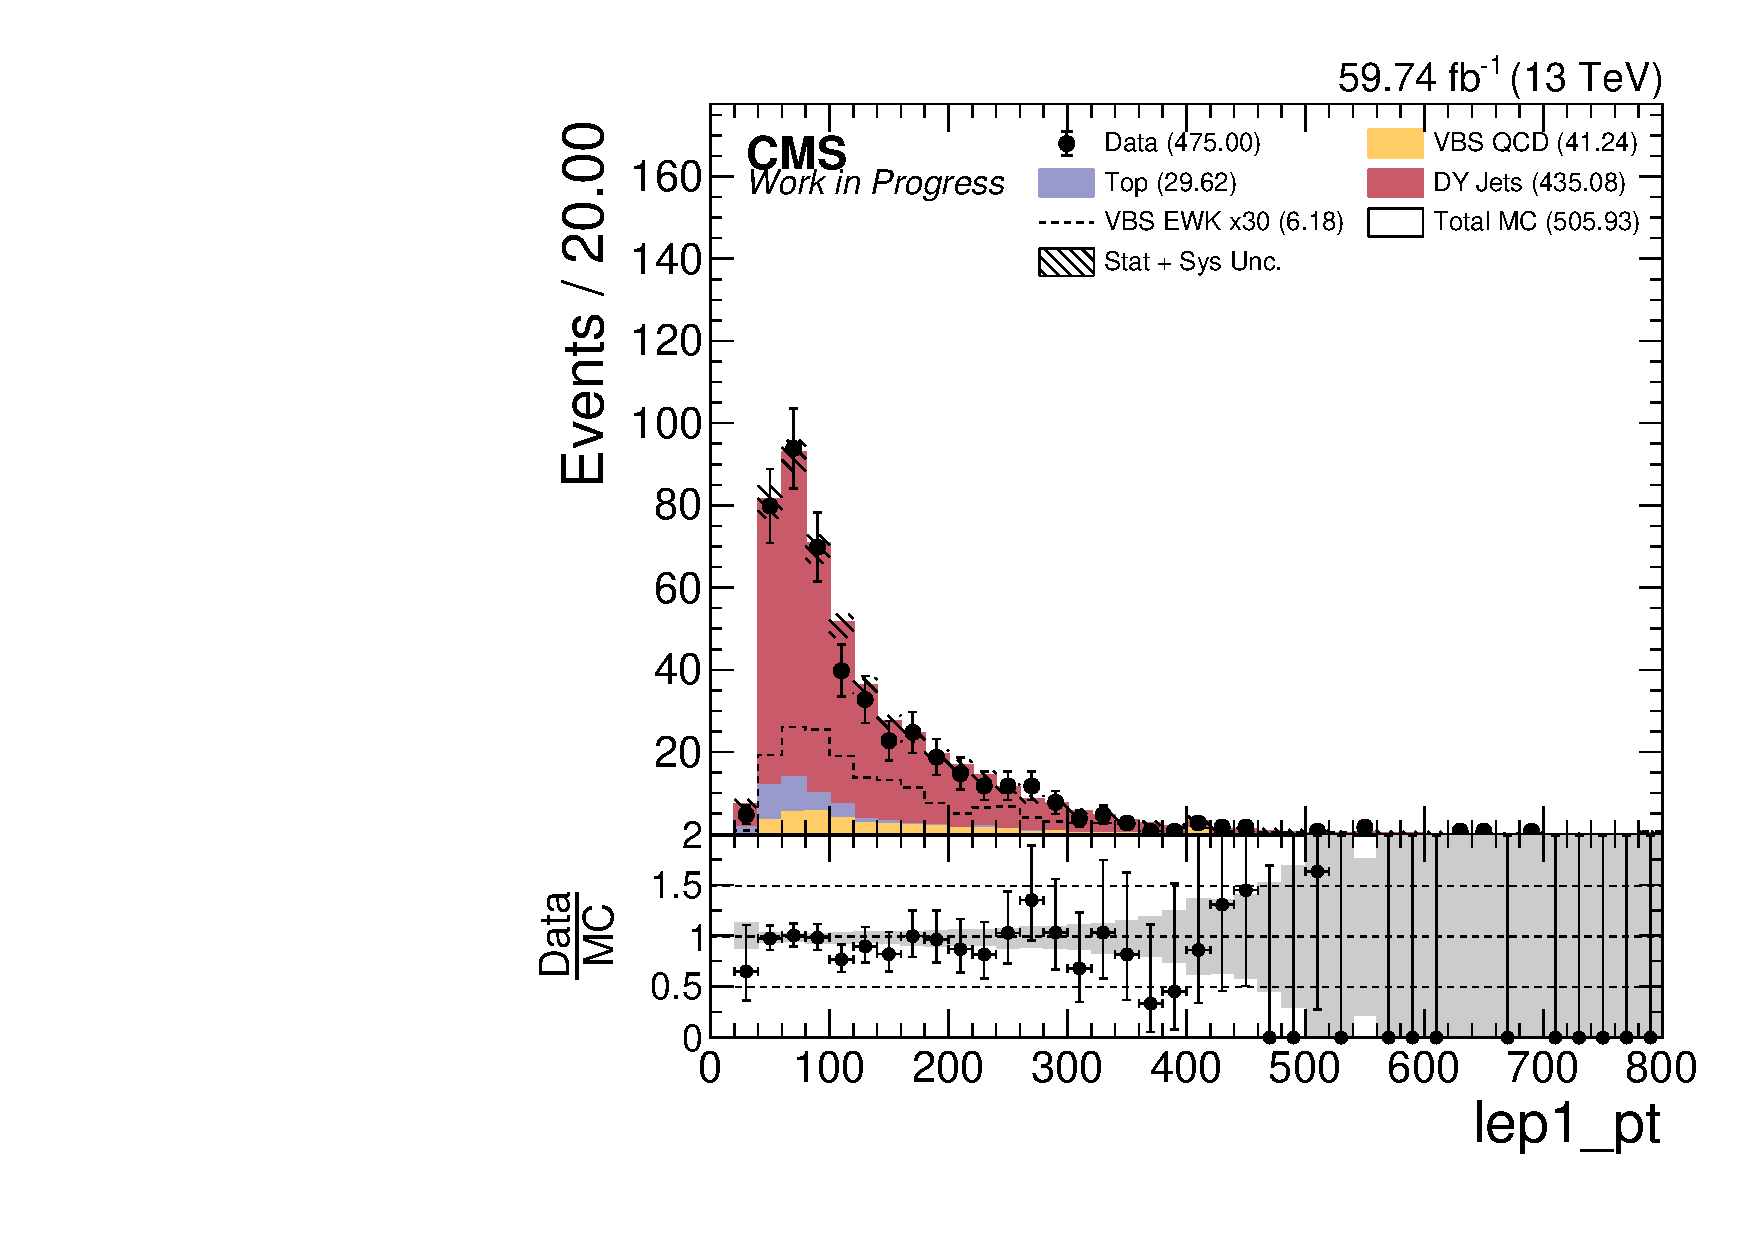
\includegraphics[width=0.335\textwidth]{analysis_plots/2018_zv/cr_vjets_m/lep1_pt.pdf} \hspace{-10pt} \\
  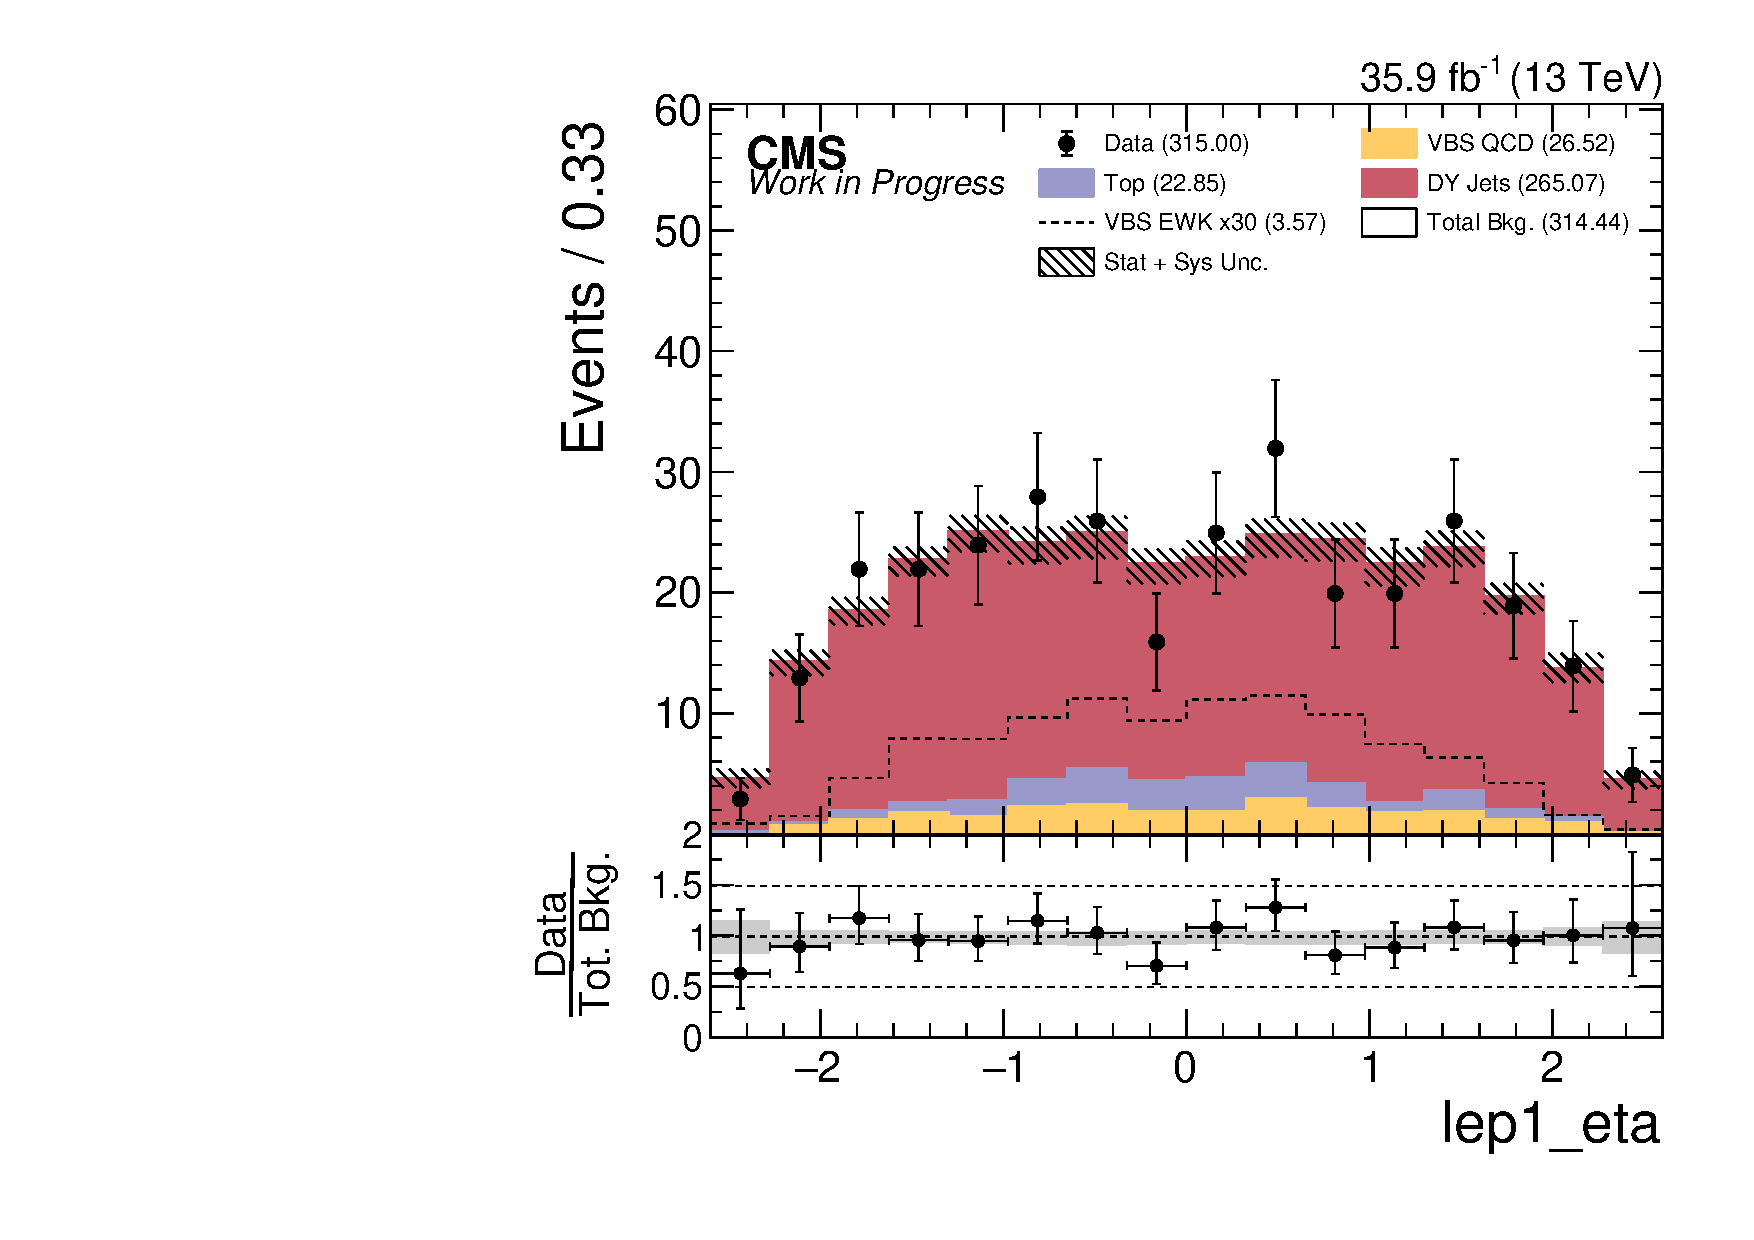
\includegraphics[width=0.335\textwidth]{analysis_plots/2016_zv/cr_vjets_m/lep1_eta.pdf} \hspace{-10pt}
  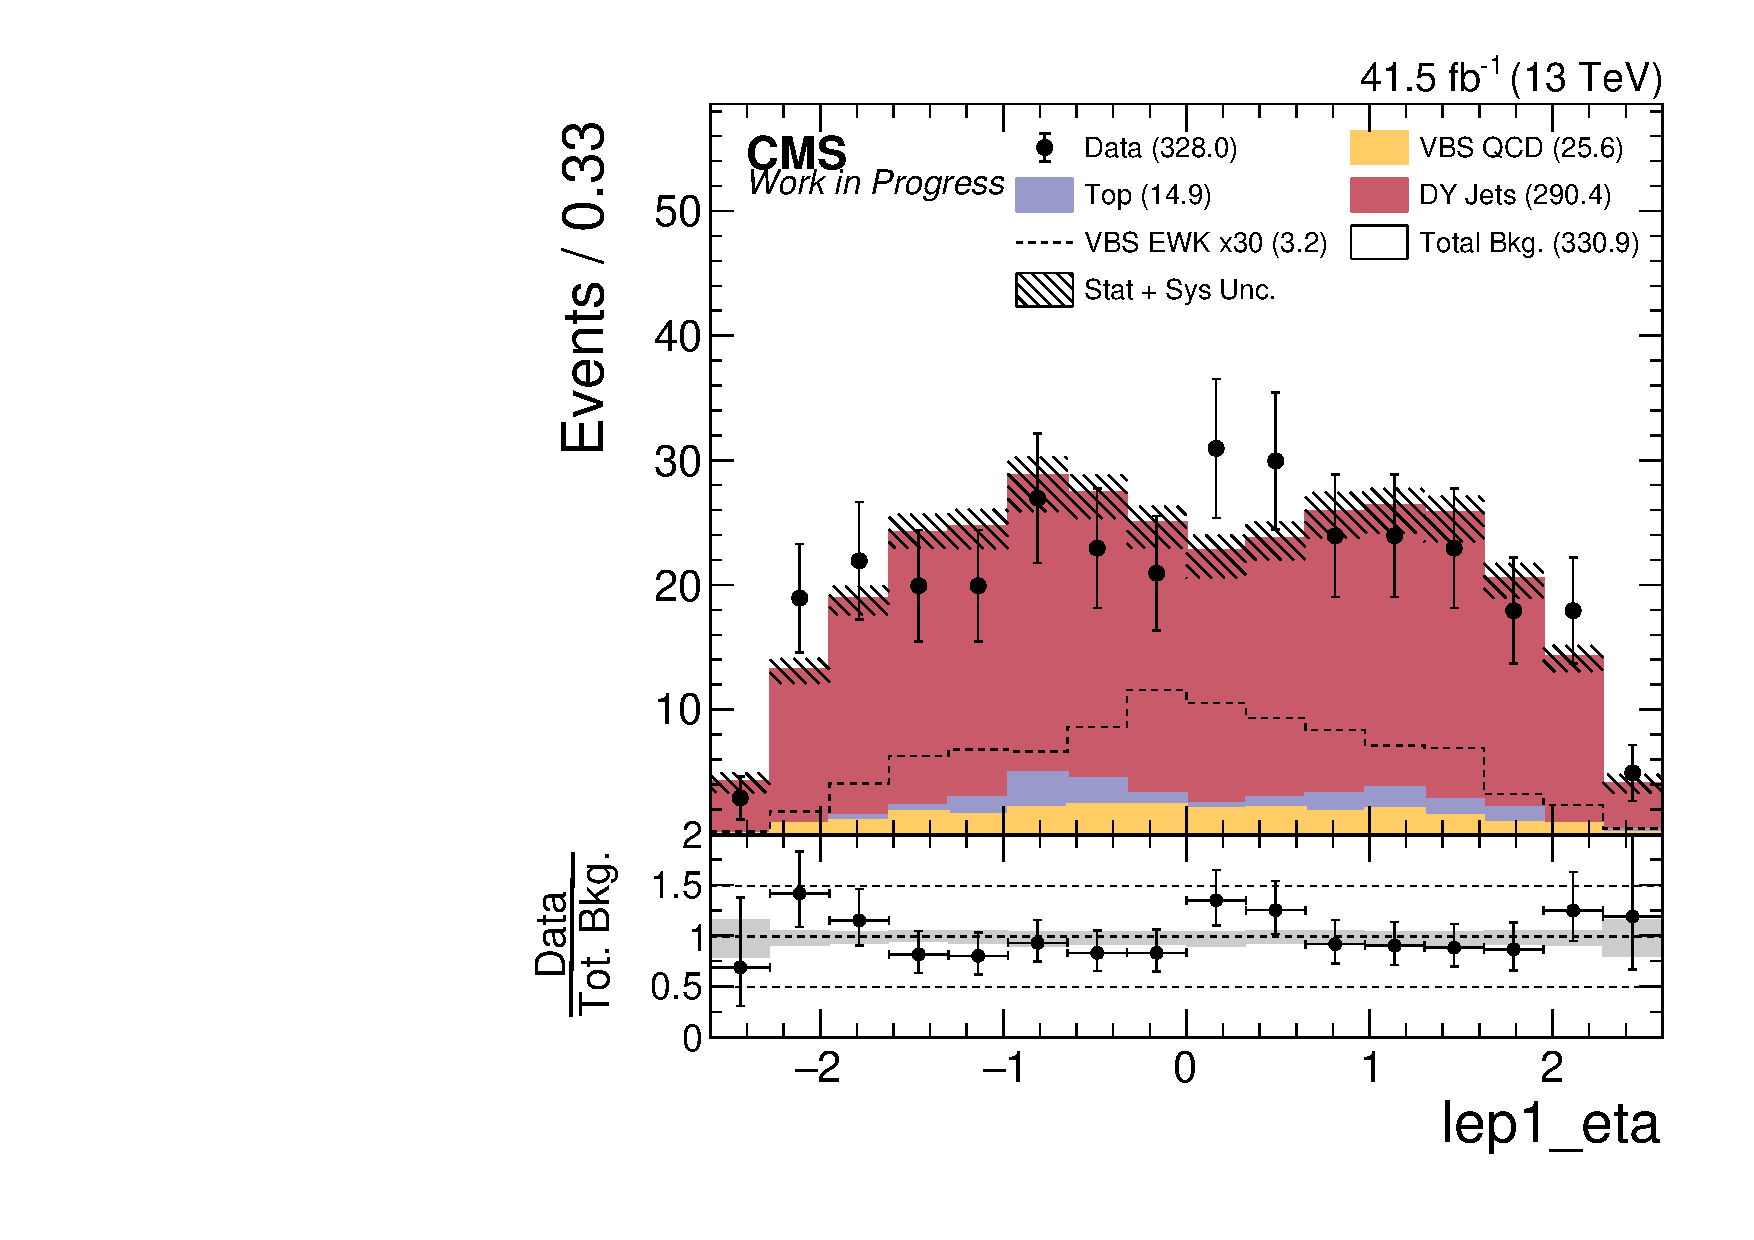
\includegraphics[width=0.335\textwidth]{analysis_plots/2017_zv/cr_vjets_m/lep1_eta.pdf} \hspace{-10pt}
  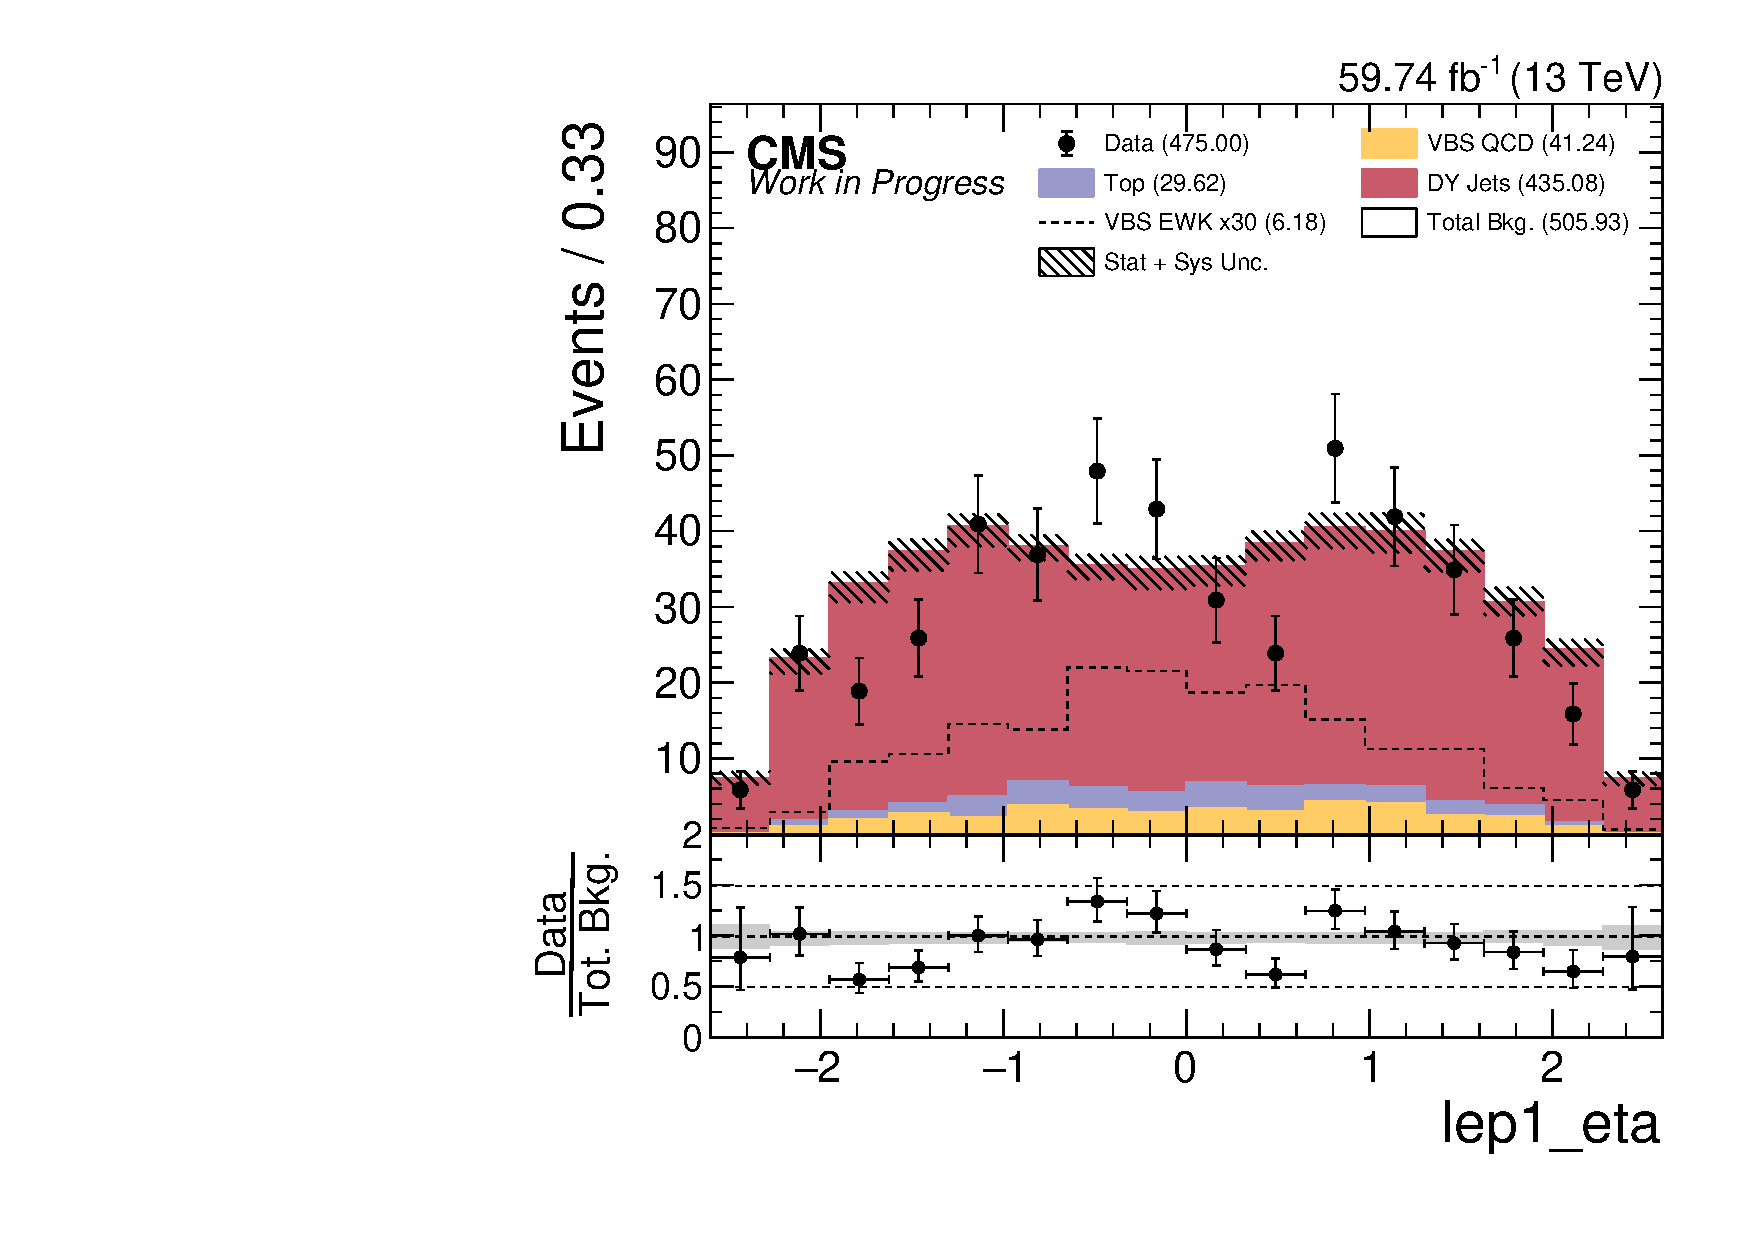
\includegraphics[width=0.335\textwidth]{analysis_plots/2018_zv/cr_vjets_m/lep1_eta.pdf} \hspace{-10pt} \\
  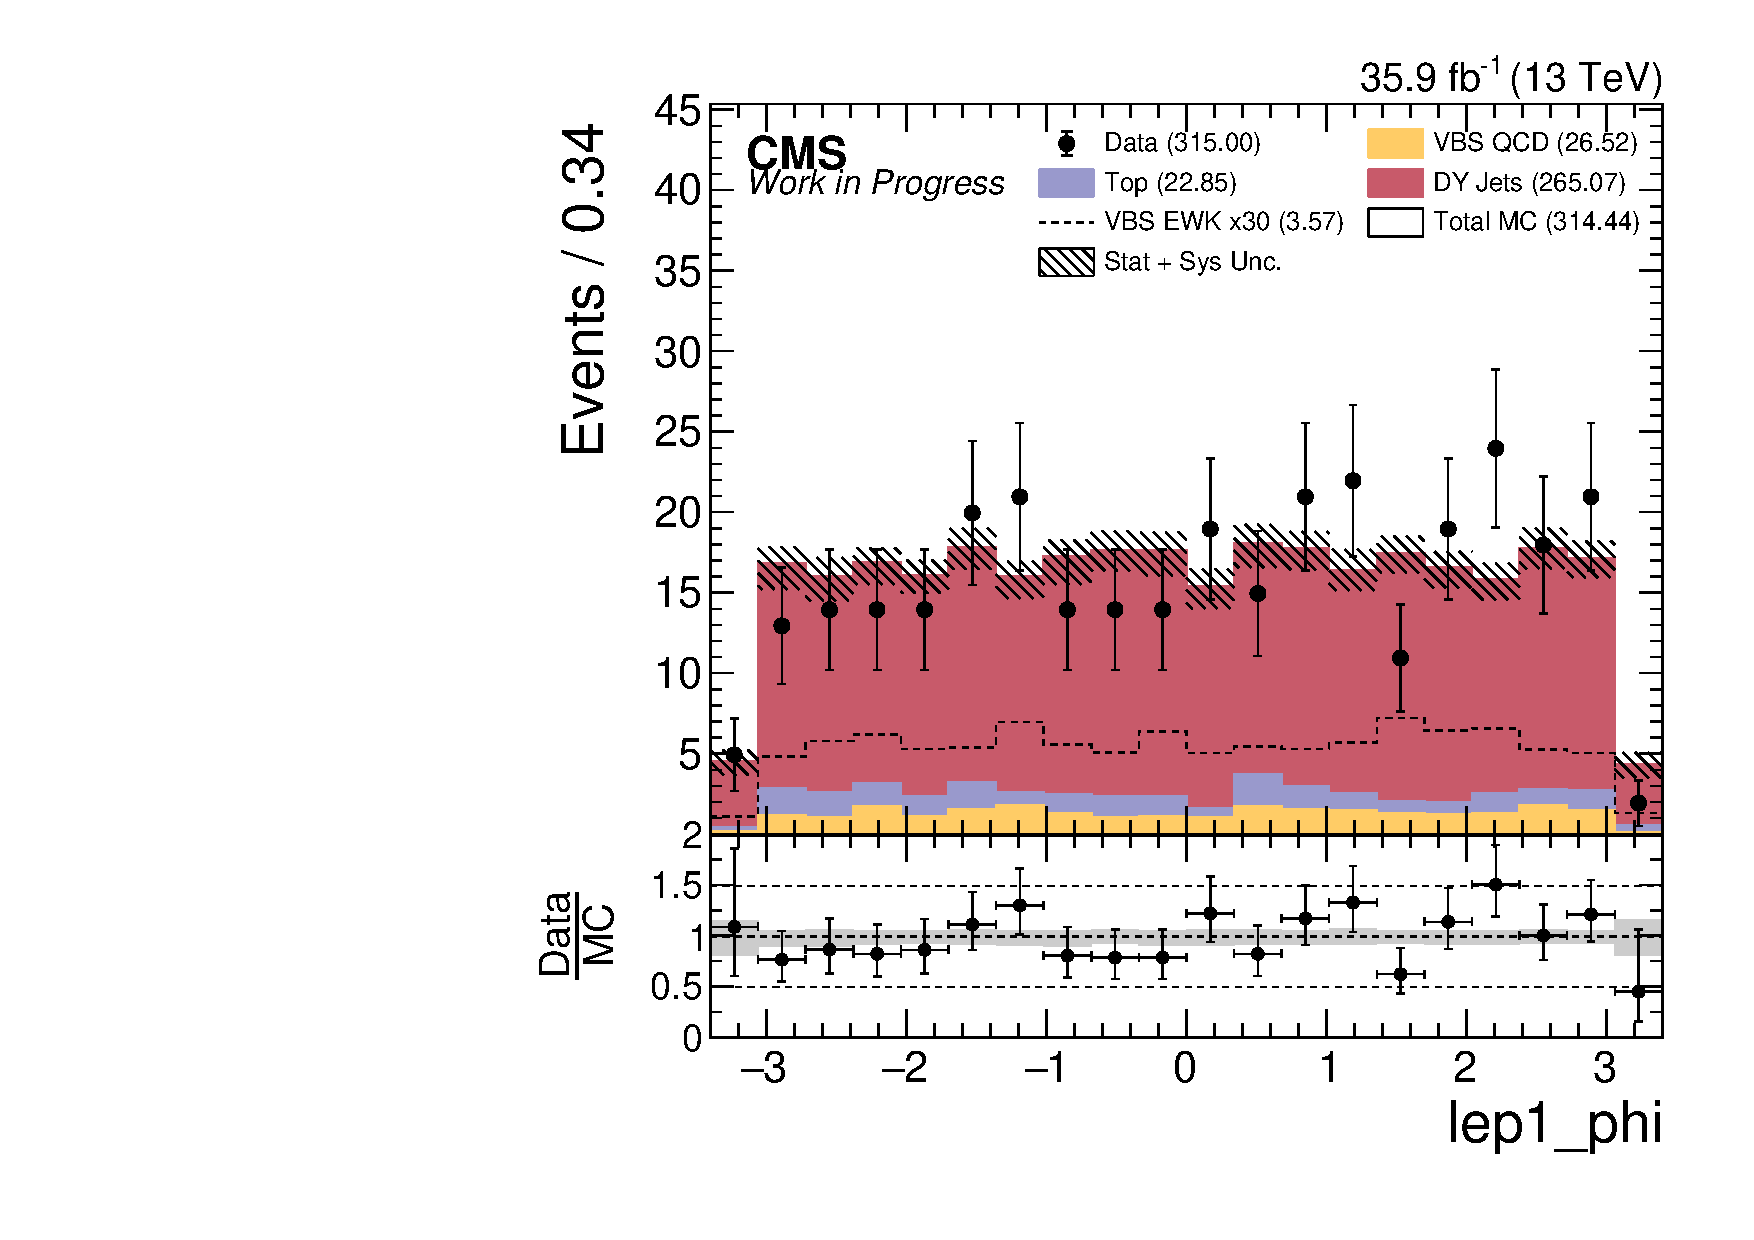
\includegraphics[width=0.335\textwidth]{analysis_plots/2016_zv/cr_vjets_m/lep1_phi.pdf} \hspace{-10pt}
  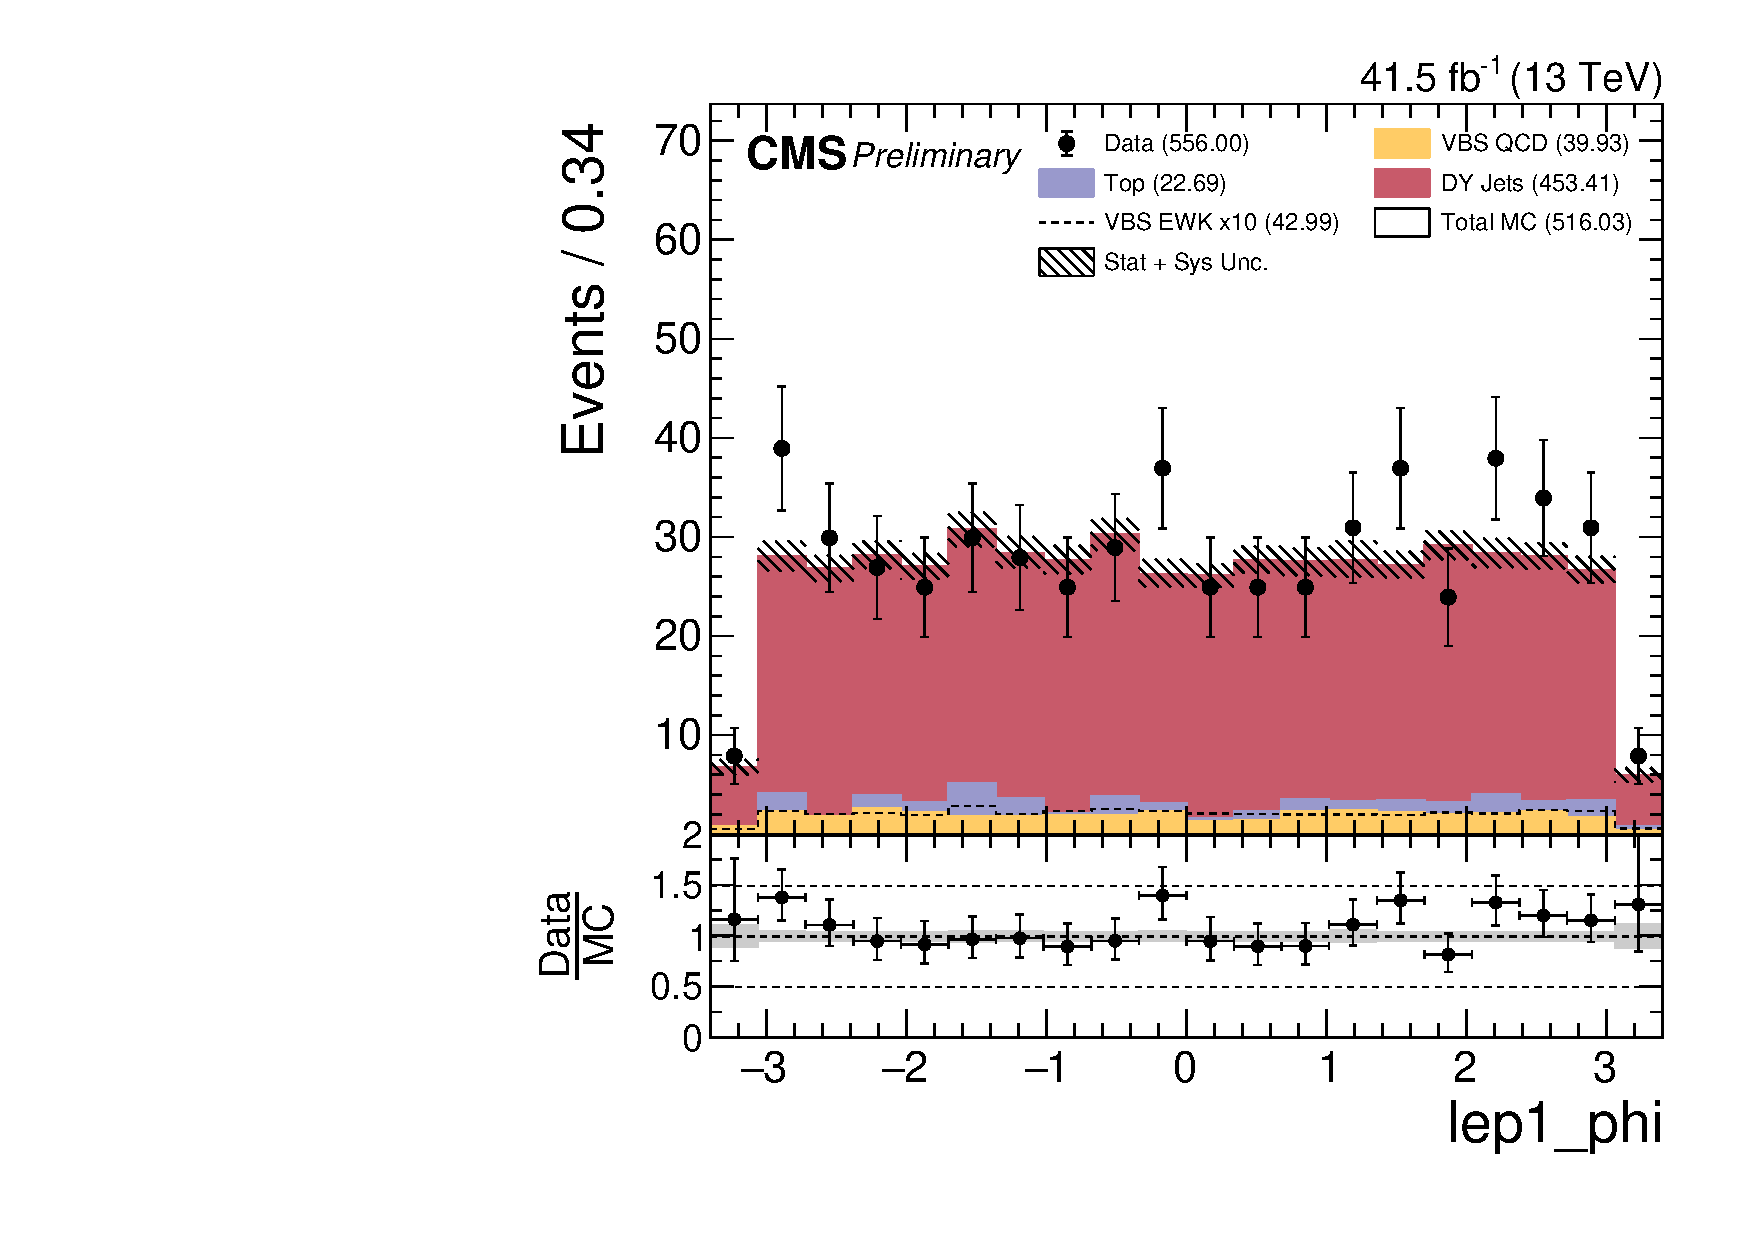
\includegraphics[width=0.335\textwidth]{analysis_plots/2017_zv/cr_vjets_m/lep1_phi.pdf} \hspace{-10pt}
  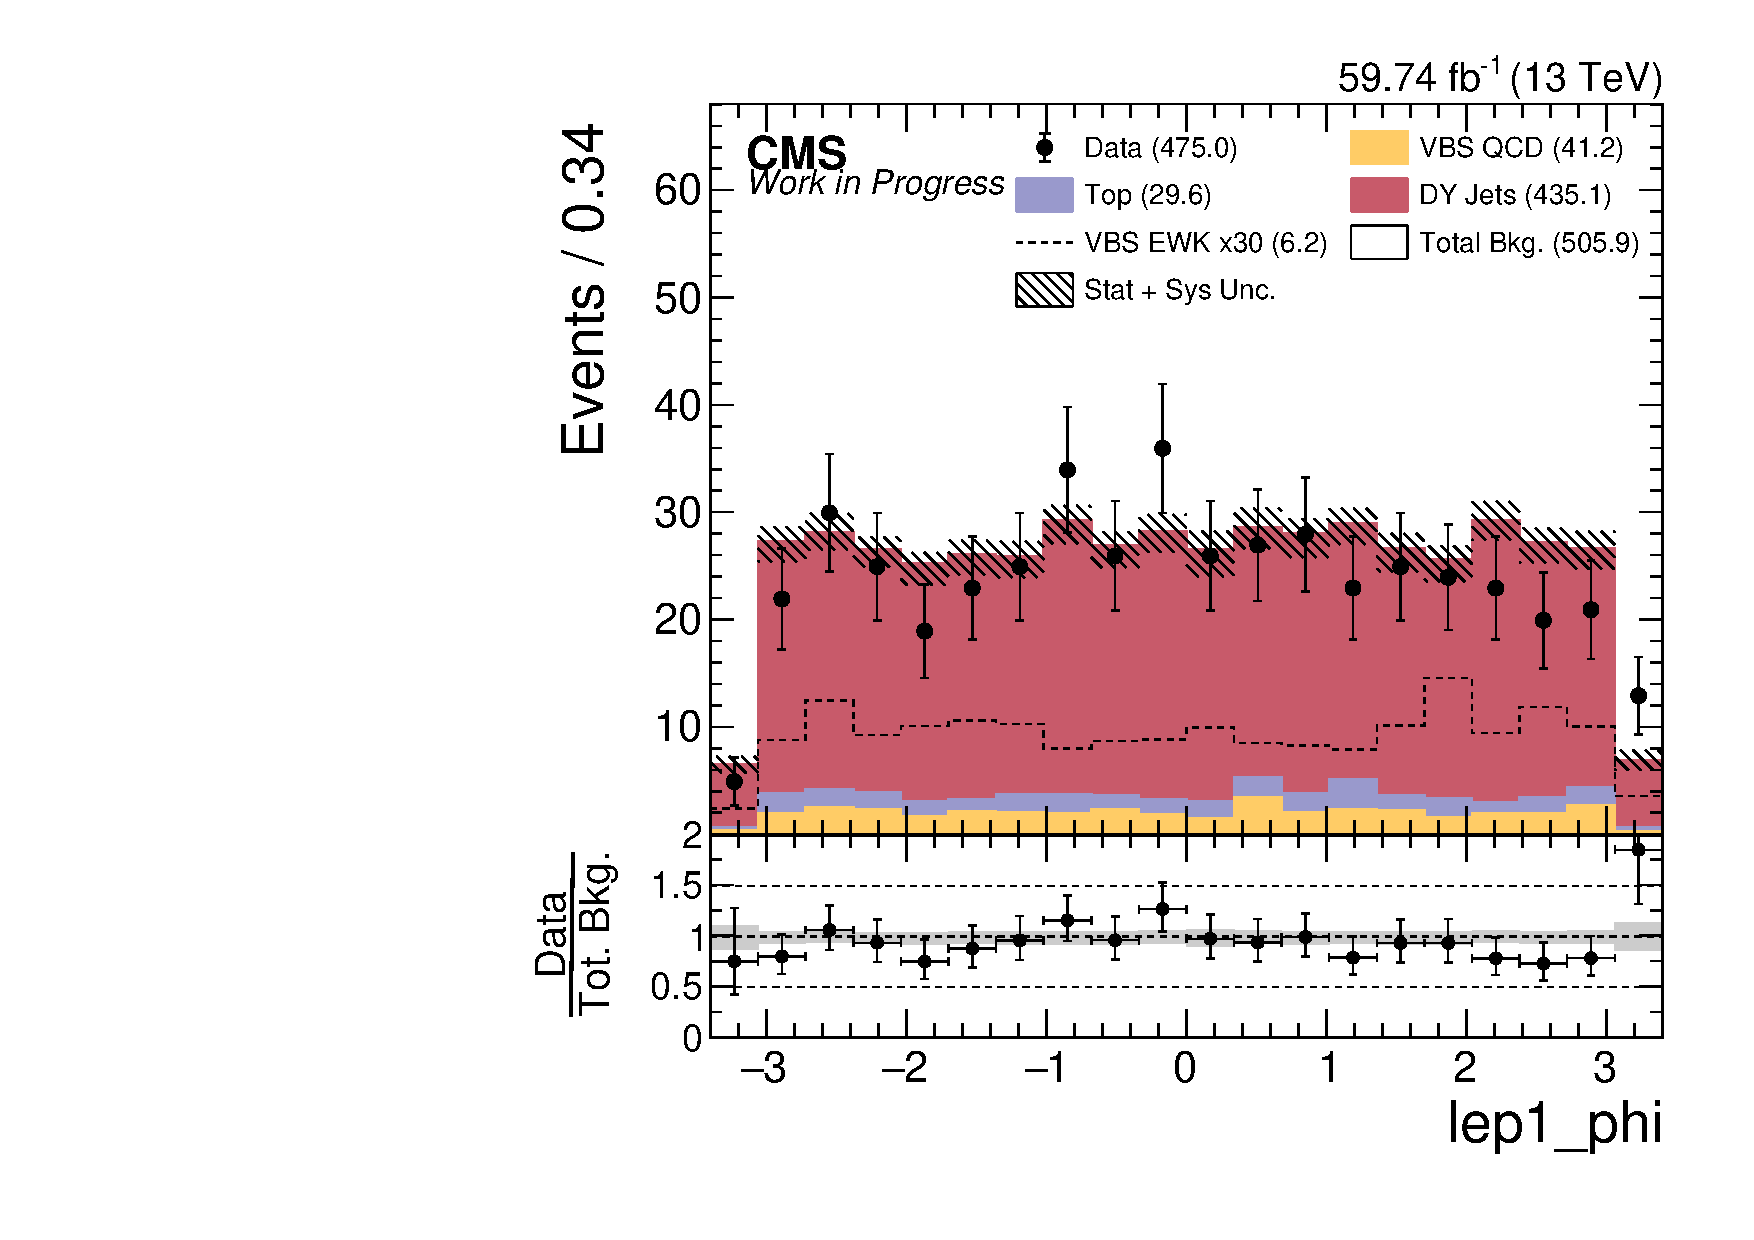
\includegraphics[width=0.335\textwidth]{analysis_plots/2018_zv/cr_vjets_m/lep1_phi.pdf} \hspace{-10pt} \\
  \caption[DY+Jets Control Region: Leading muon kinematics in Boosted ZV Channel]%
  {DY+Jets Control Region: Leading muon kinematics in Boosted ZV Channel.
    Error bars include statistical uncertainty on total background,
    JES and QCD scale systematic on DY+Jets and VBS\_QCD MC\@. From Left to Right: 2016,
    2017, and 2018. From Top to Bottom: \( p_T \), \( \eta \), and \( \phi \).}%
  \label{fig:zv-cr-vjets-m-lep1-pt-eta-phi}
\end{figure}

\begin{figure}[!ht]
  \centering
  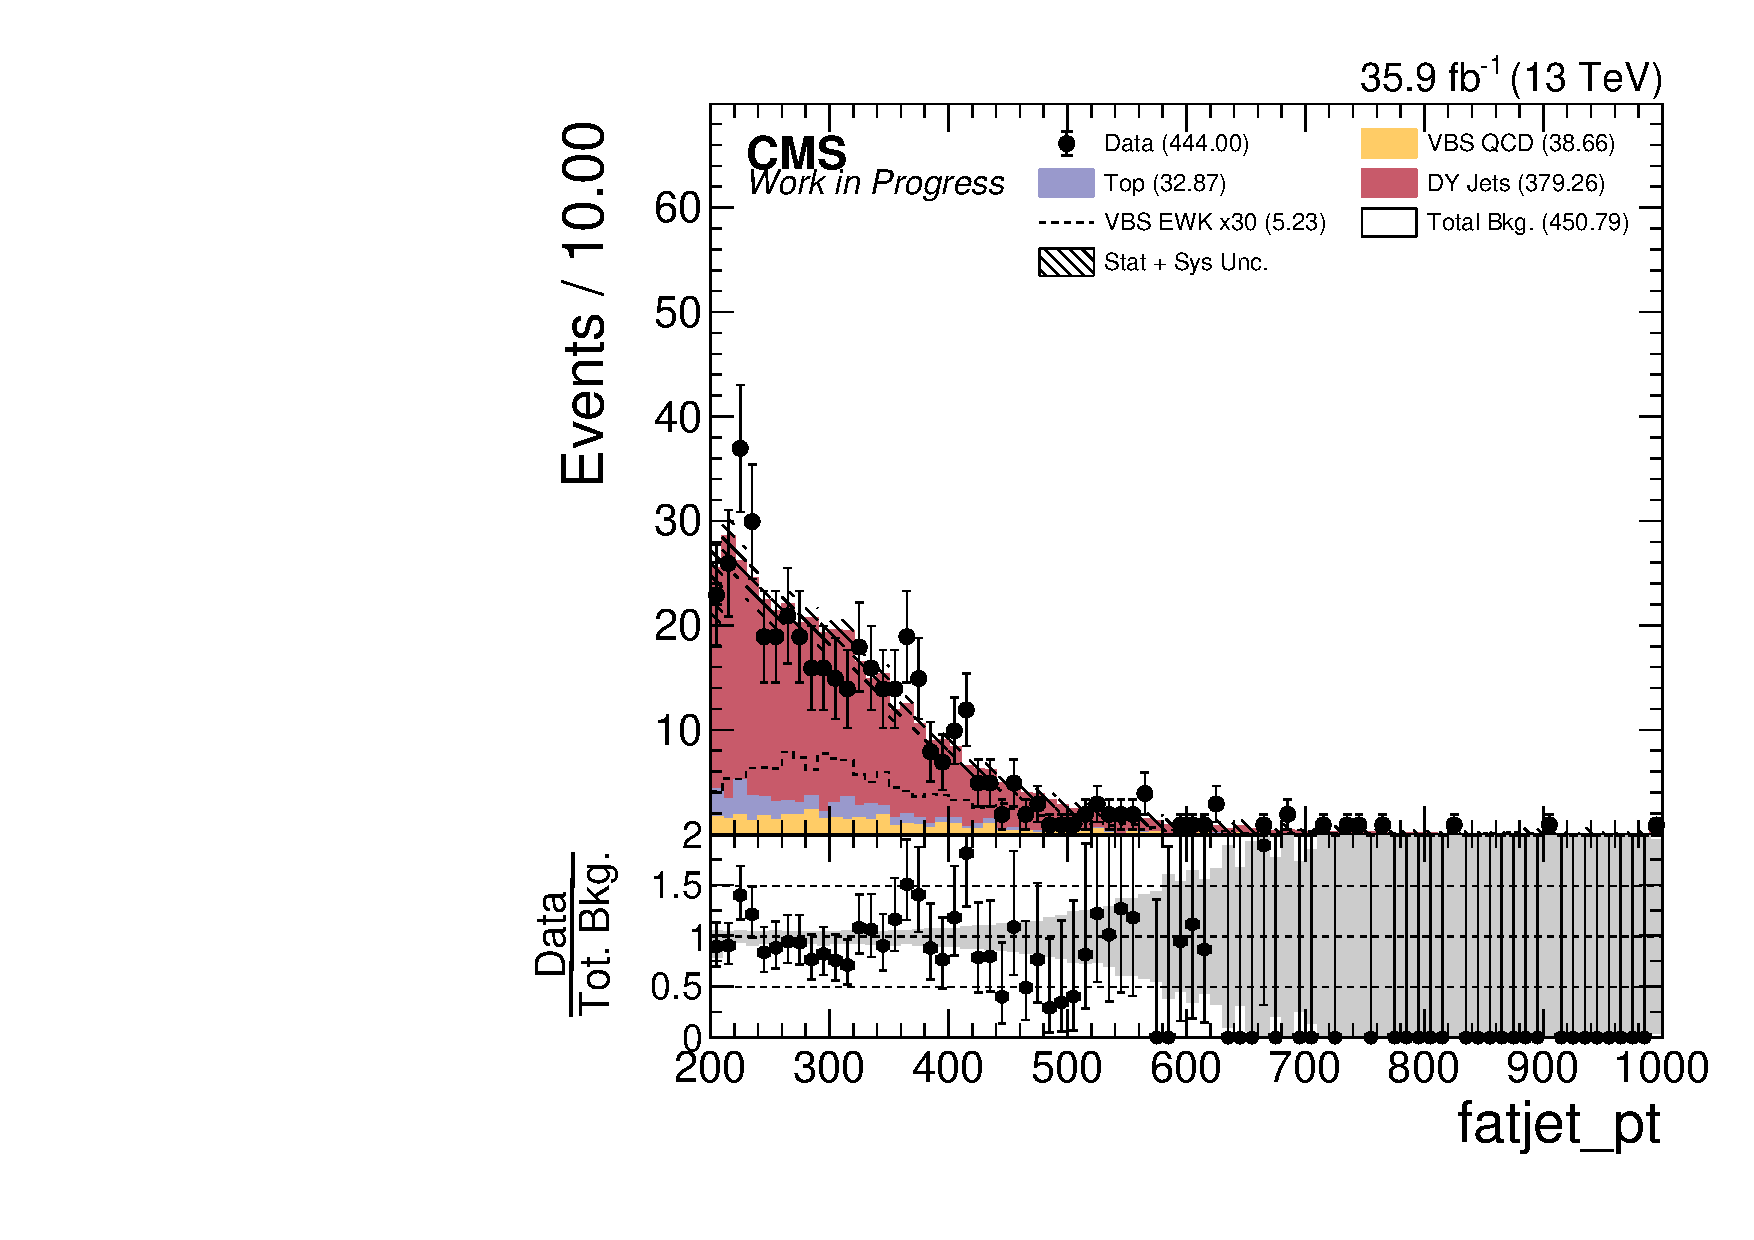
\includegraphics[width=0.335\textwidth]{analysis_plots/2016_zv/cr_vjets_l/fatjet_pt.pdf} \hspace{-10pt}
  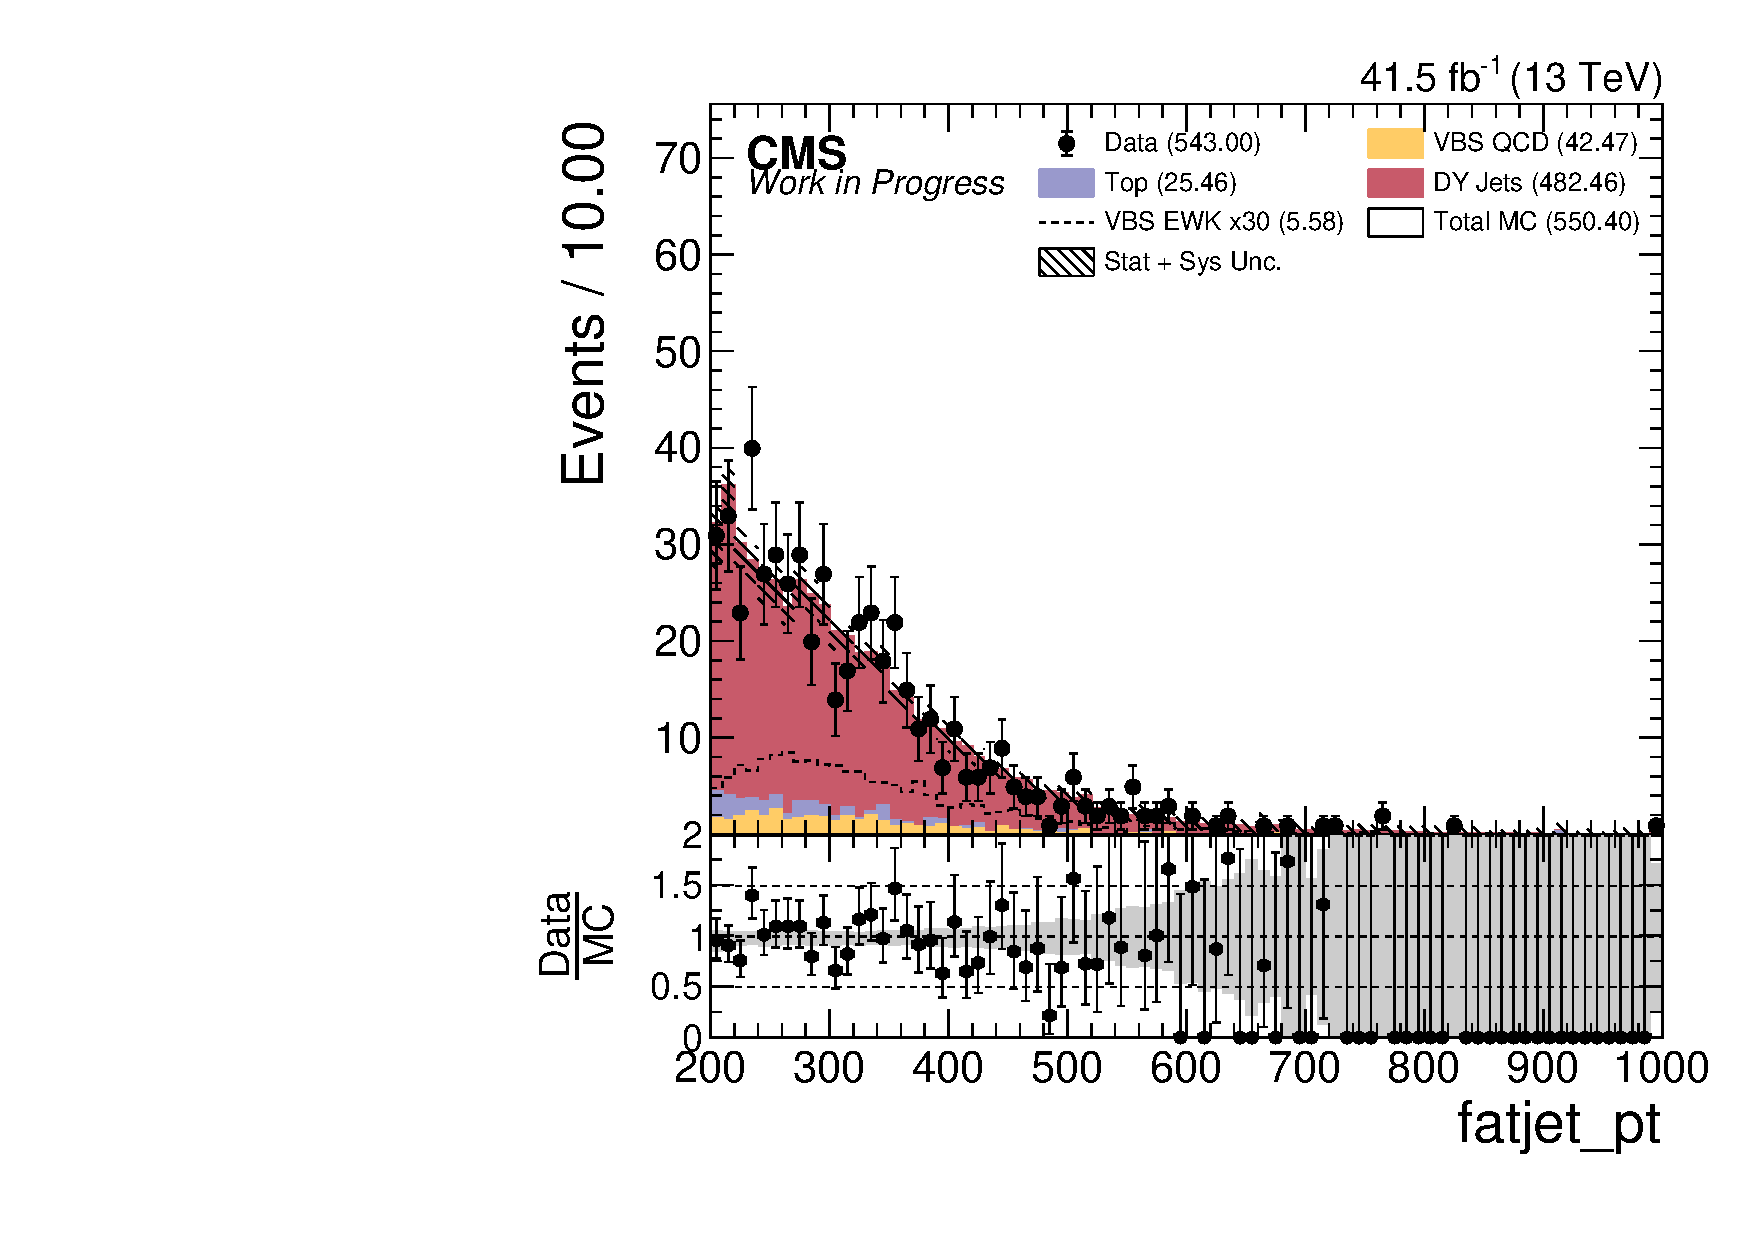
\includegraphics[width=0.335\textwidth]{analysis_plots/2017_zv/cr_vjets_l/fatjet_pt.pdf} \hspace{-10pt}
  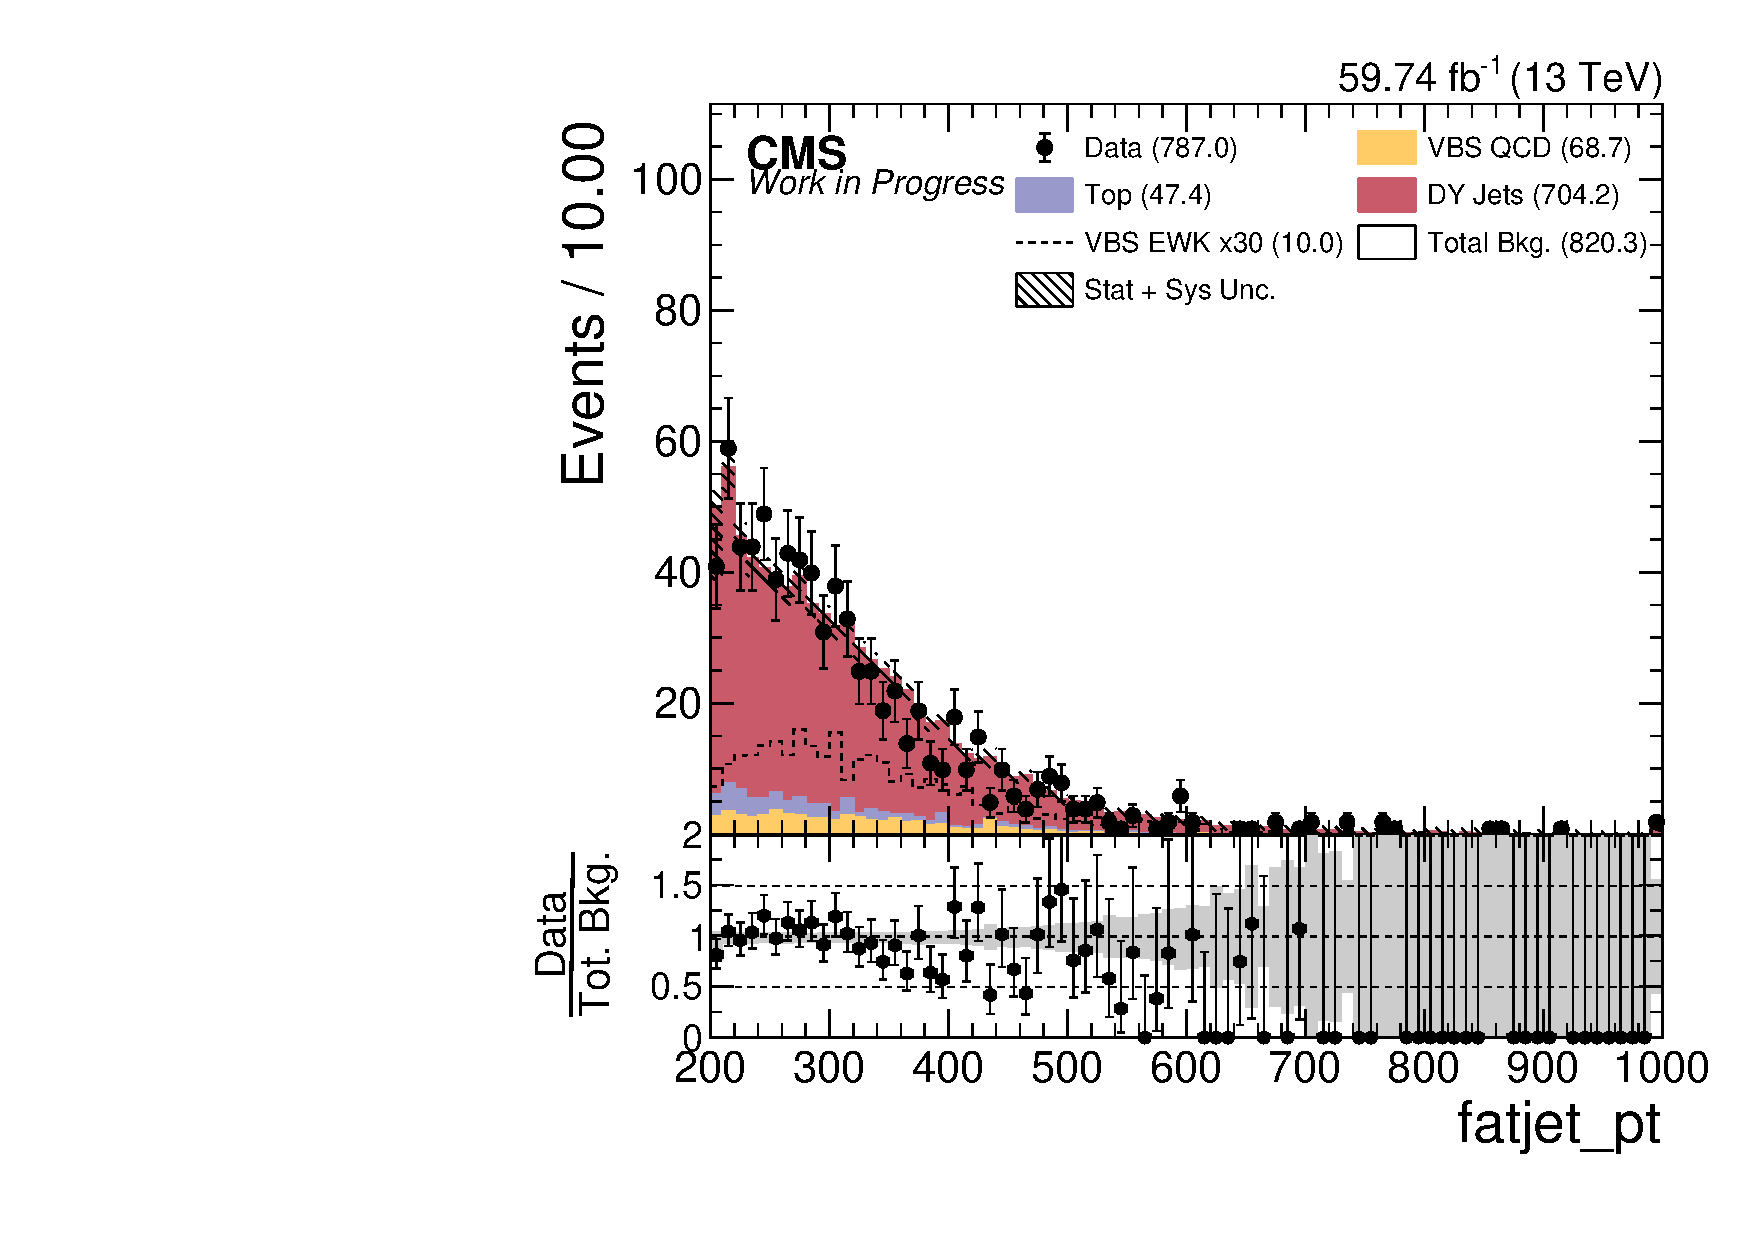
\includegraphics[width=0.335\textwidth]{analysis_plots/2018_zv/cr_vjets_l/fatjet_pt.pdf} \hspace{-10pt} \\
  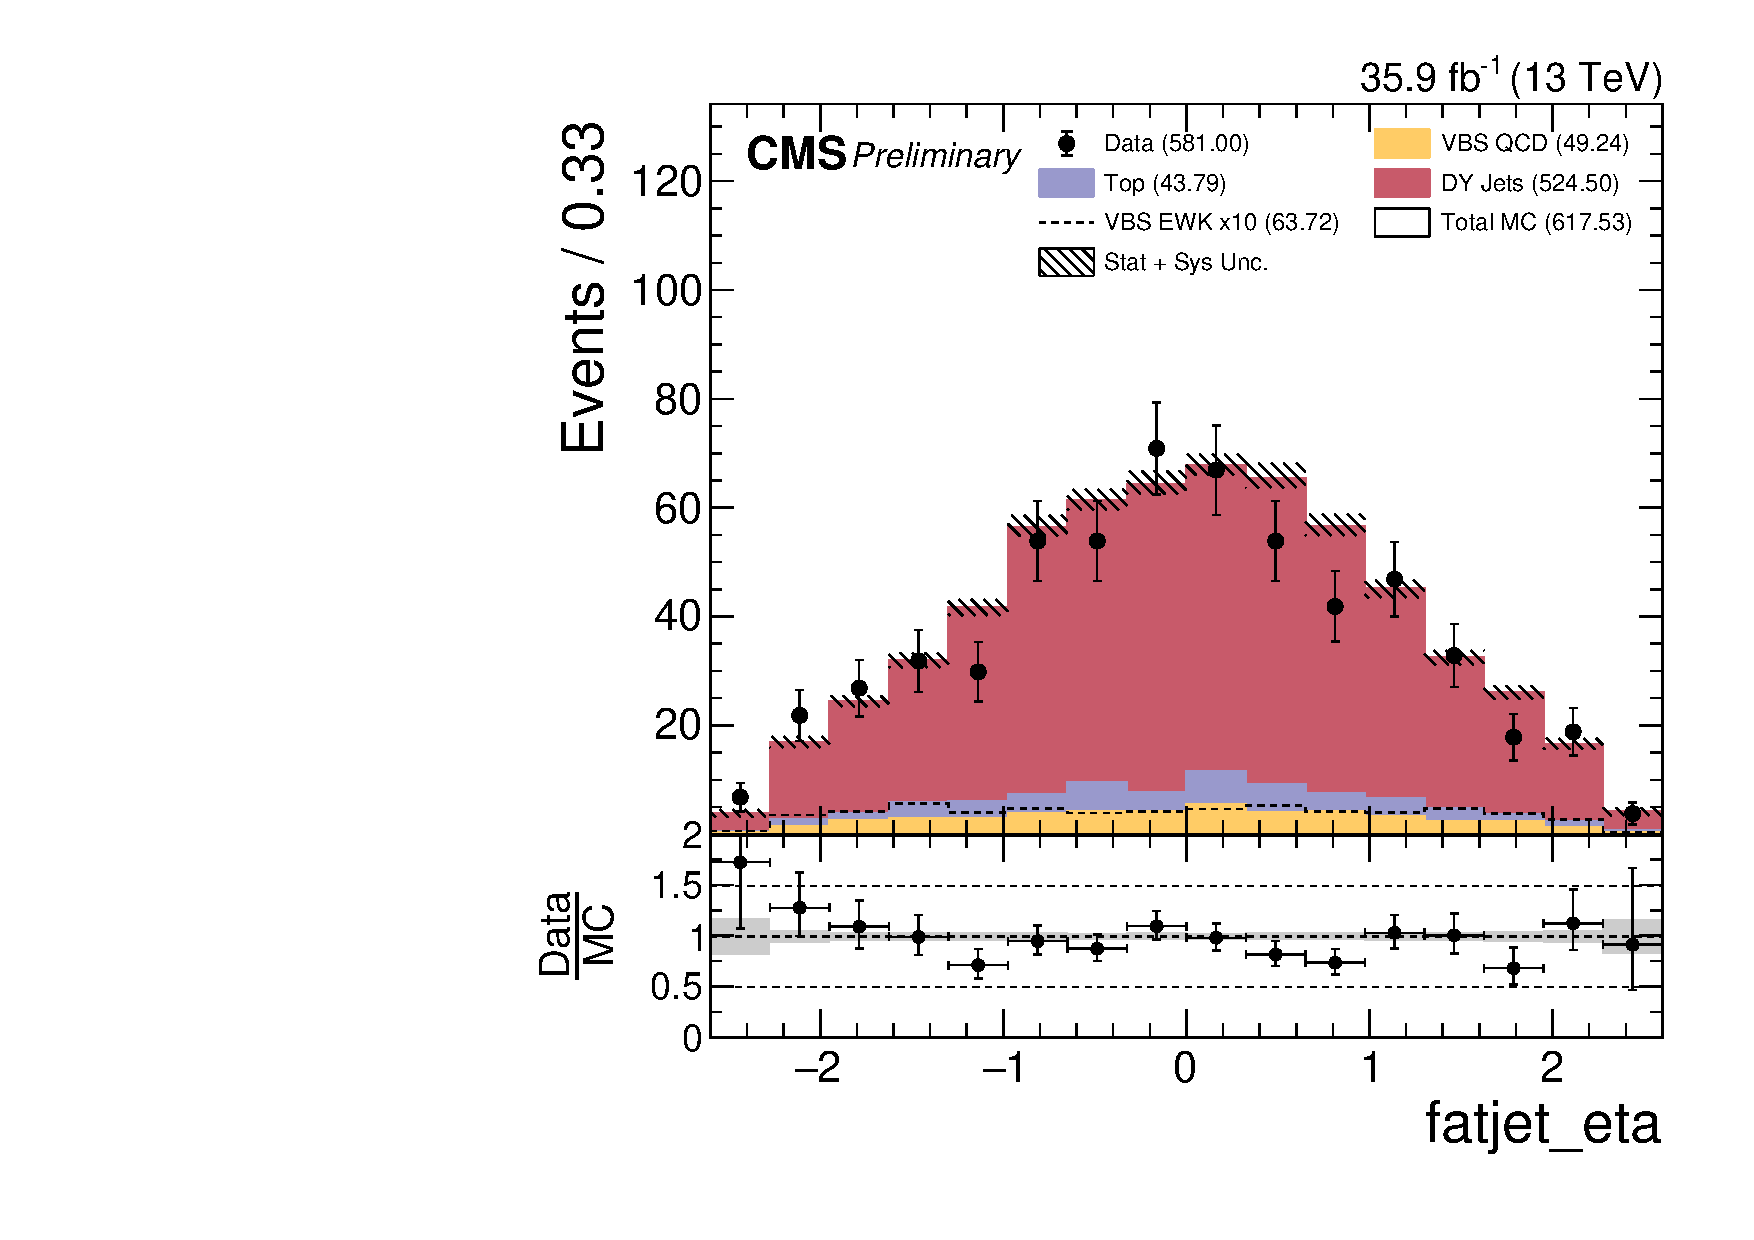
\includegraphics[width=0.335\textwidth]{analysis_plots/2016_zv/cr_vjets_l/fatjet_eta.pdf} \hspace{-10pt}
  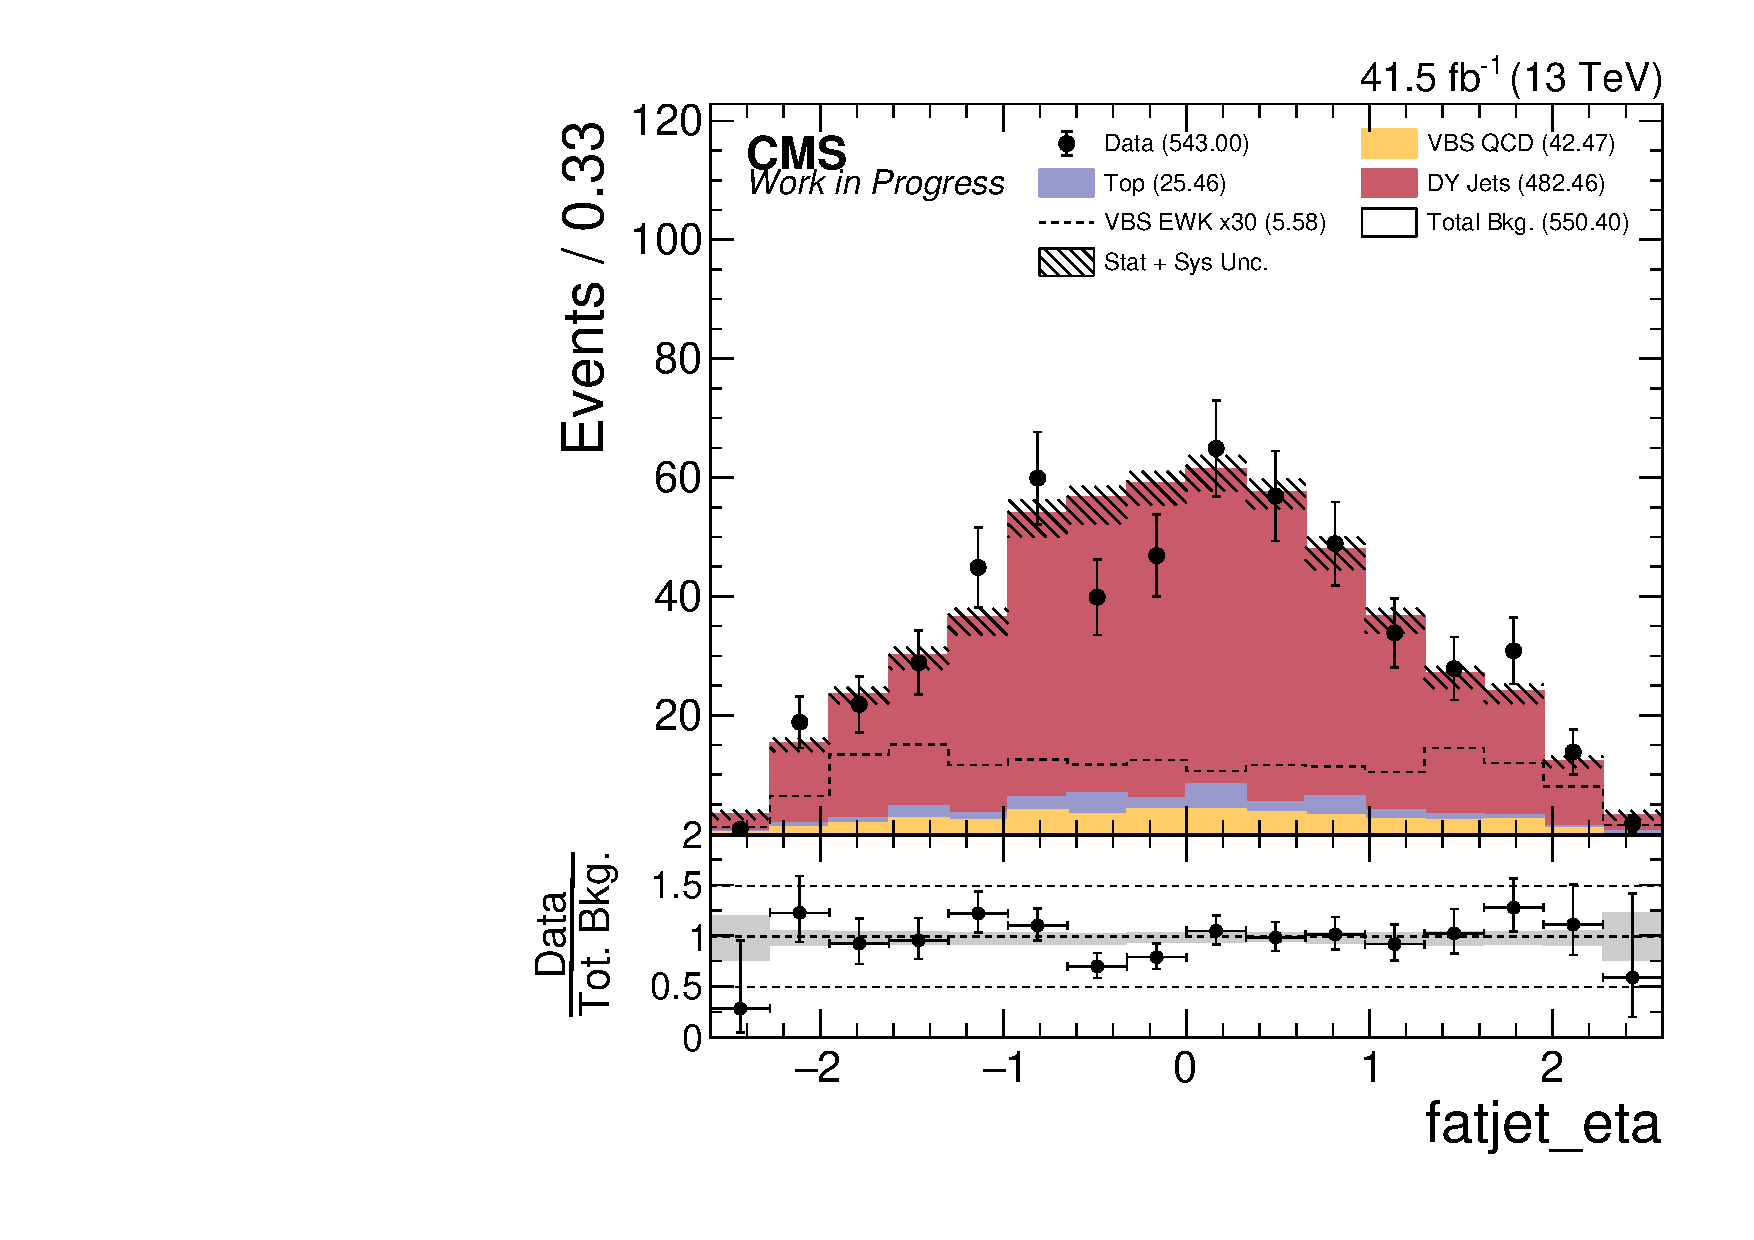
\includegraphics[width=0.335\textwidth]{analysis_plots/2017_zv/cr_vjets_l/fatjet_eta.pdf} \hspace{-10pt}
  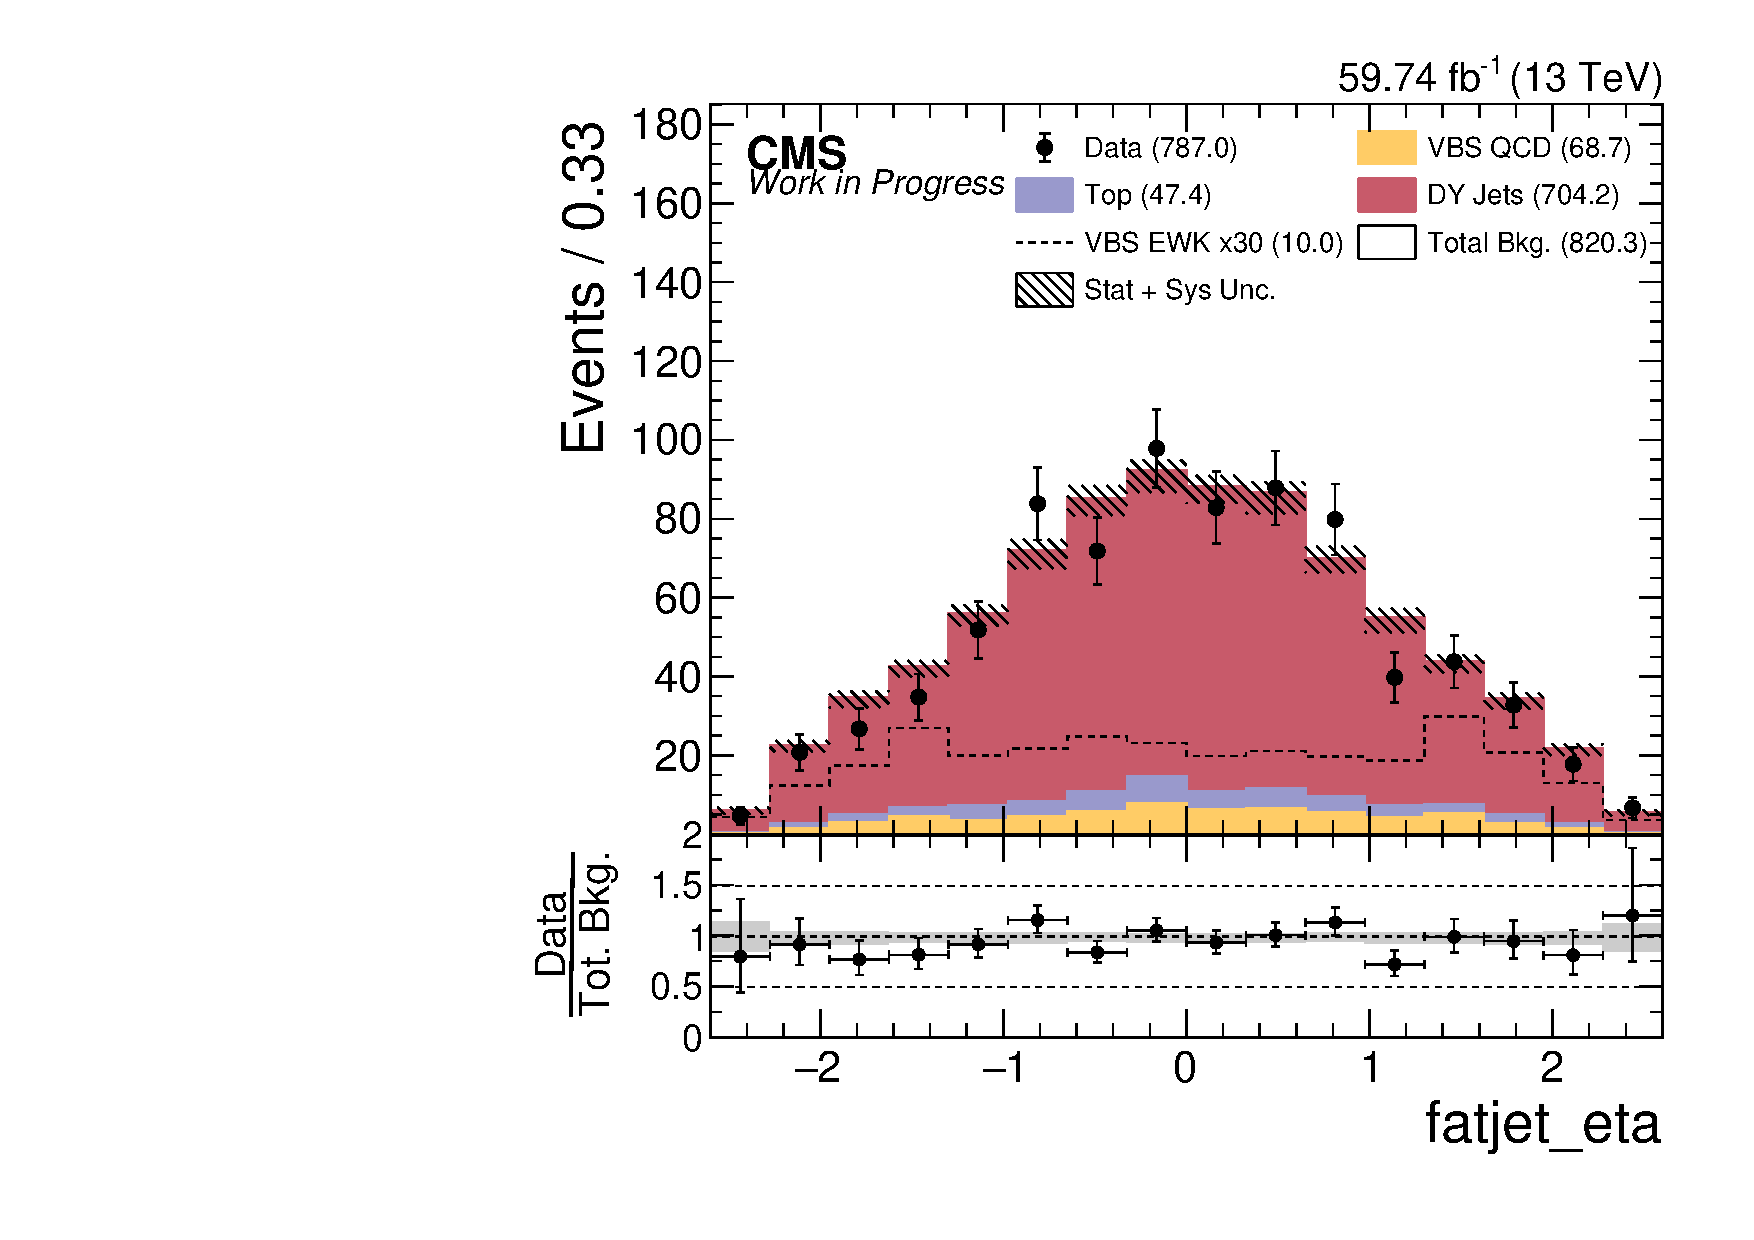
\includegraphics[width=0.335\textwidth]{analysis_plots/2018_zv/cr_vjets_l/fatjet_eta.pdf} \hspace{-10pt} \\
  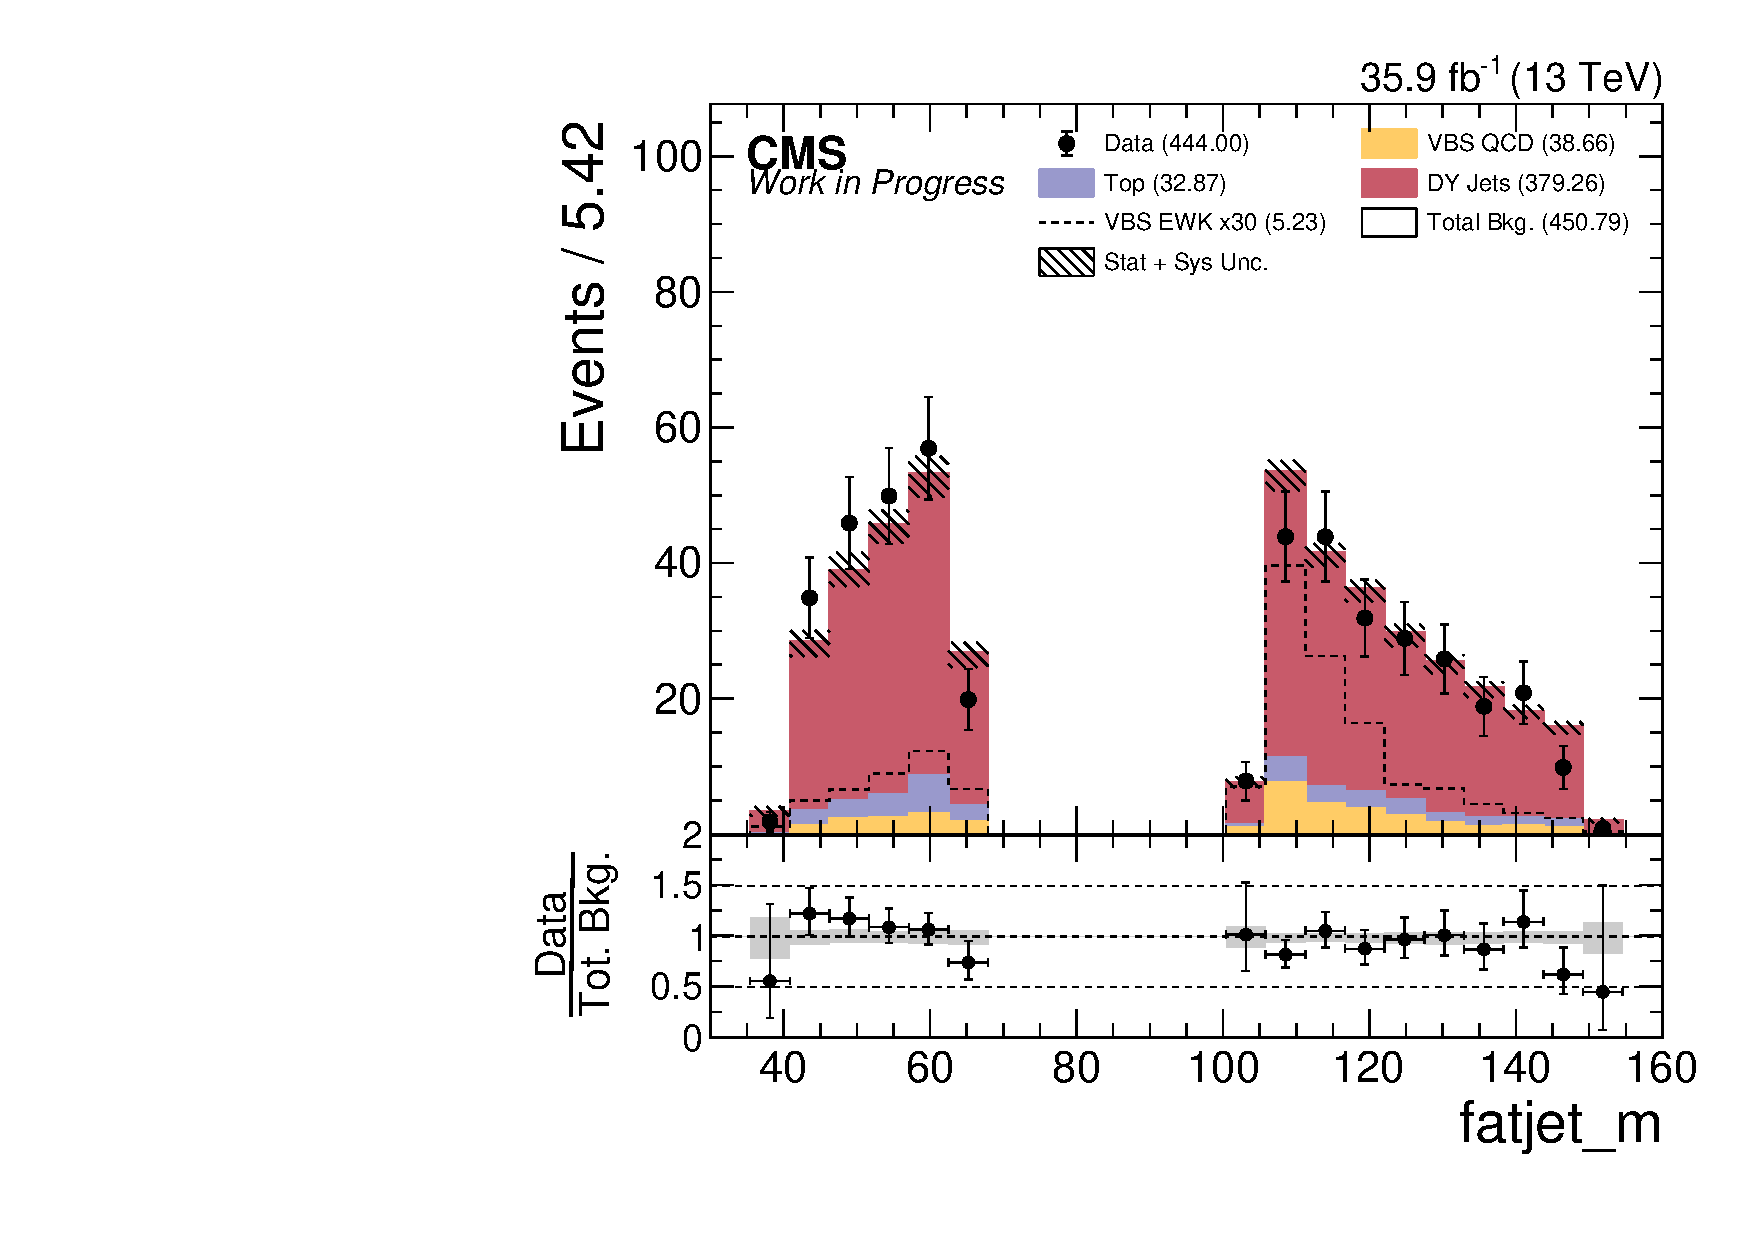
\includegraphics[width=0.335\textwidth]{analysis_plots/2016_zv/cr_vjets_l/fatjet_m.pdf} \hspace{-10pt}
  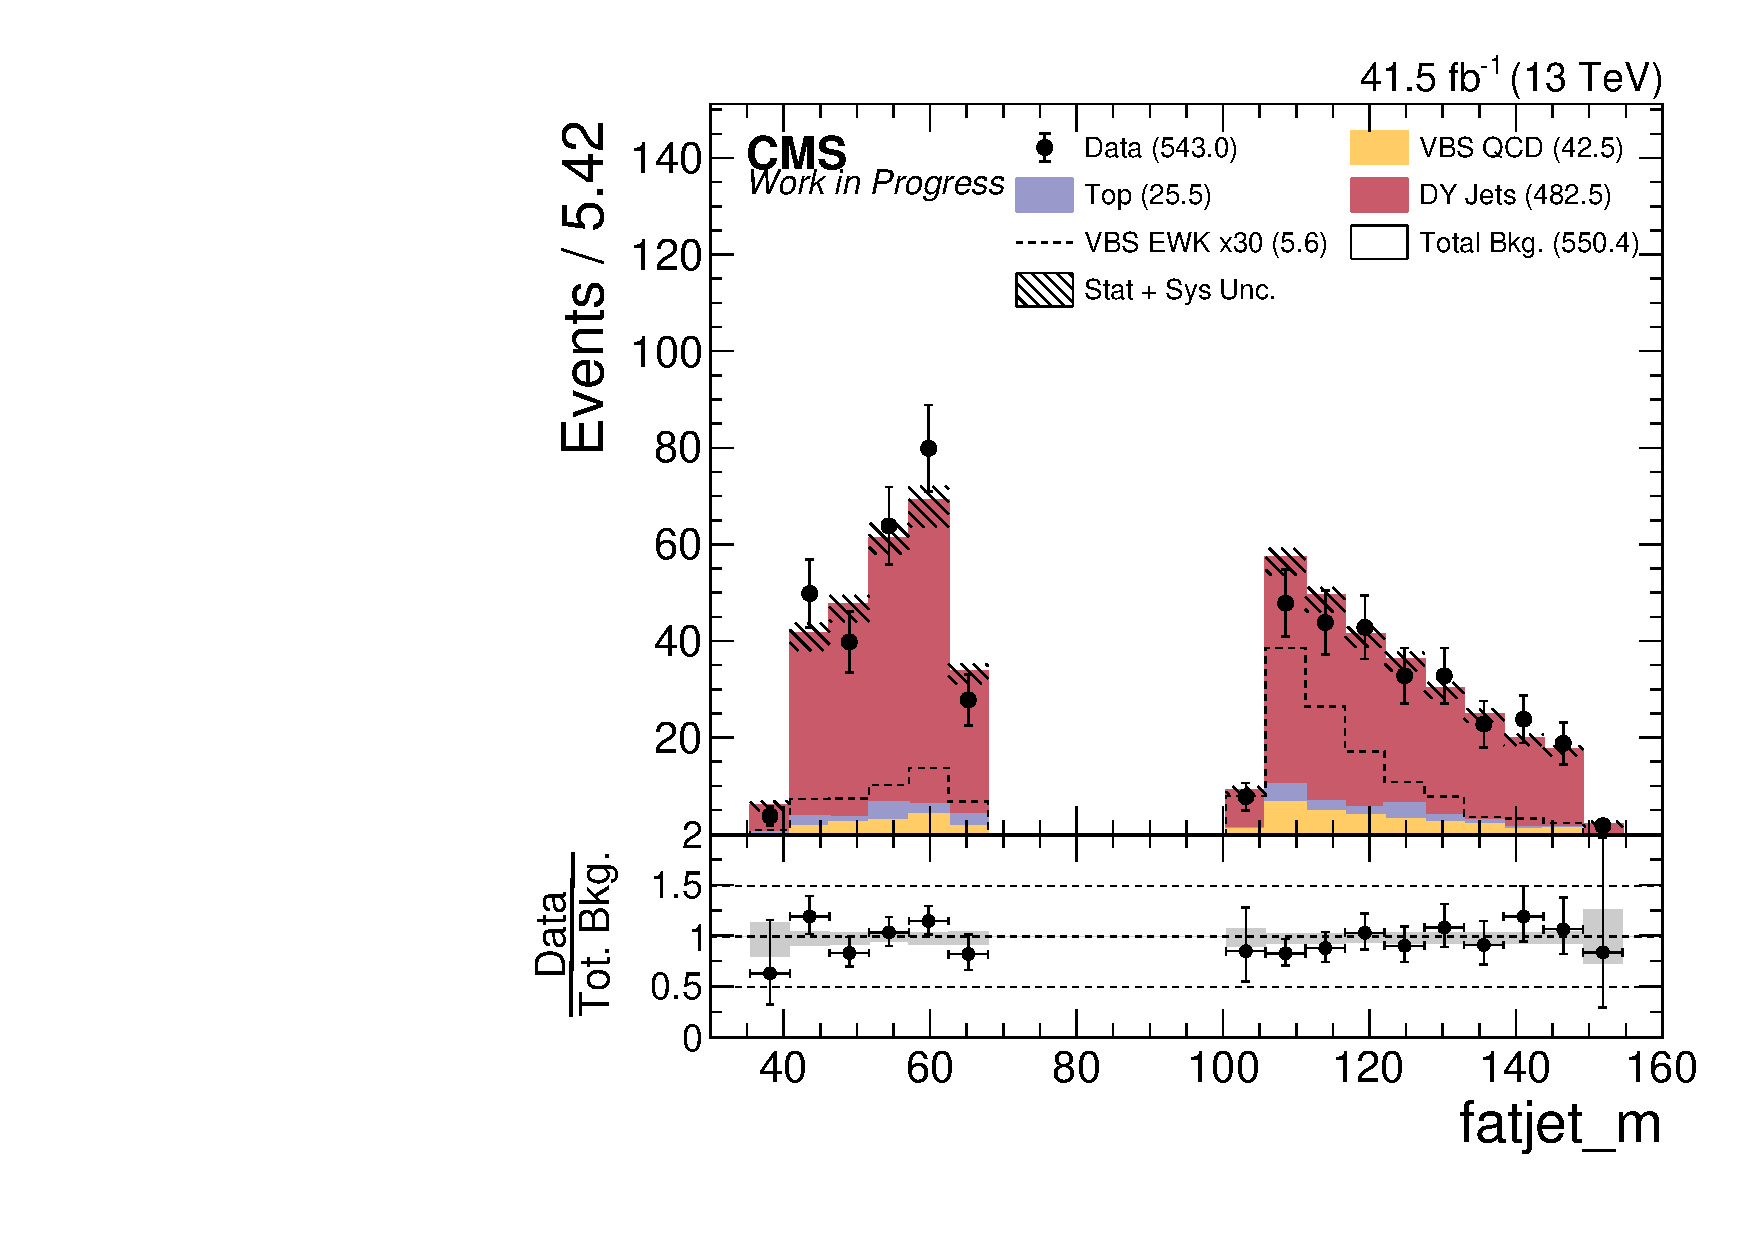
\includegraphics[width=0.335\textwidth]{analysis_plots/2017_zv/cr_vjets_l/fatjet_m.pdf} \hspace{-10pt}
  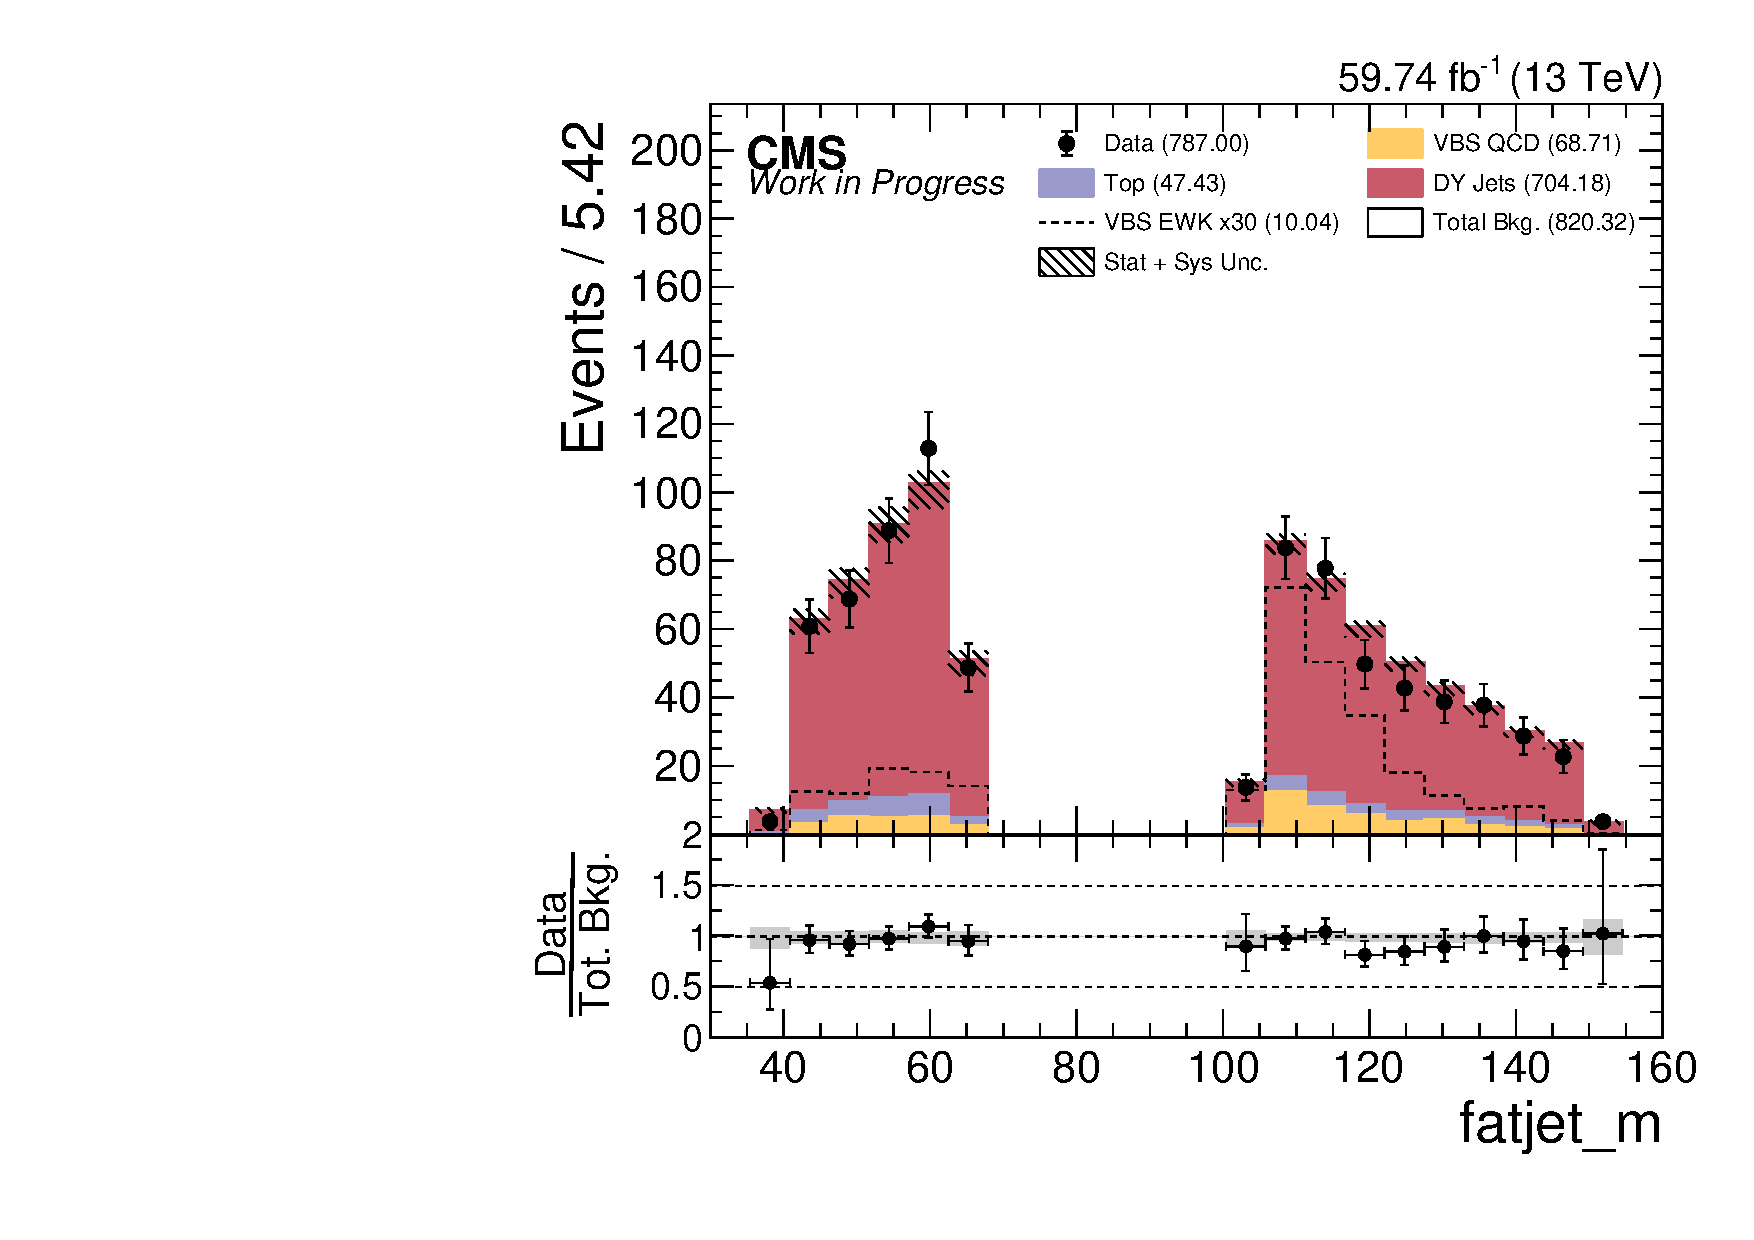
\includegraphics[width=0.335\textwidth]{analysis_plots/2018_zv/cr_vjets_l/fatjet_m.pdf} \hspace{-10pt} \\
  \caption[DY+Jets Control Region: Hadronic boson kinematics in Boosted ZV Channel]%
  {DY+Jets Control Region: Hadronic boson kinematics in Boosted ZV Channel.
    Error bars include statistical uncertainty on total background,
    JES and QCD scale systematic on DY+Jets and VBS\_QCD MC\@. From Left to Right: 2016,
    2017, and 2018. From Top to Bottom: \( p_T \), \( \eta \), and mass \( m \).}%
  \label{fig:zv-cr-vjets-l-fatjet-pt-eta-m}
\end{figure}

\begin{figure}[!ht]
  \centering
  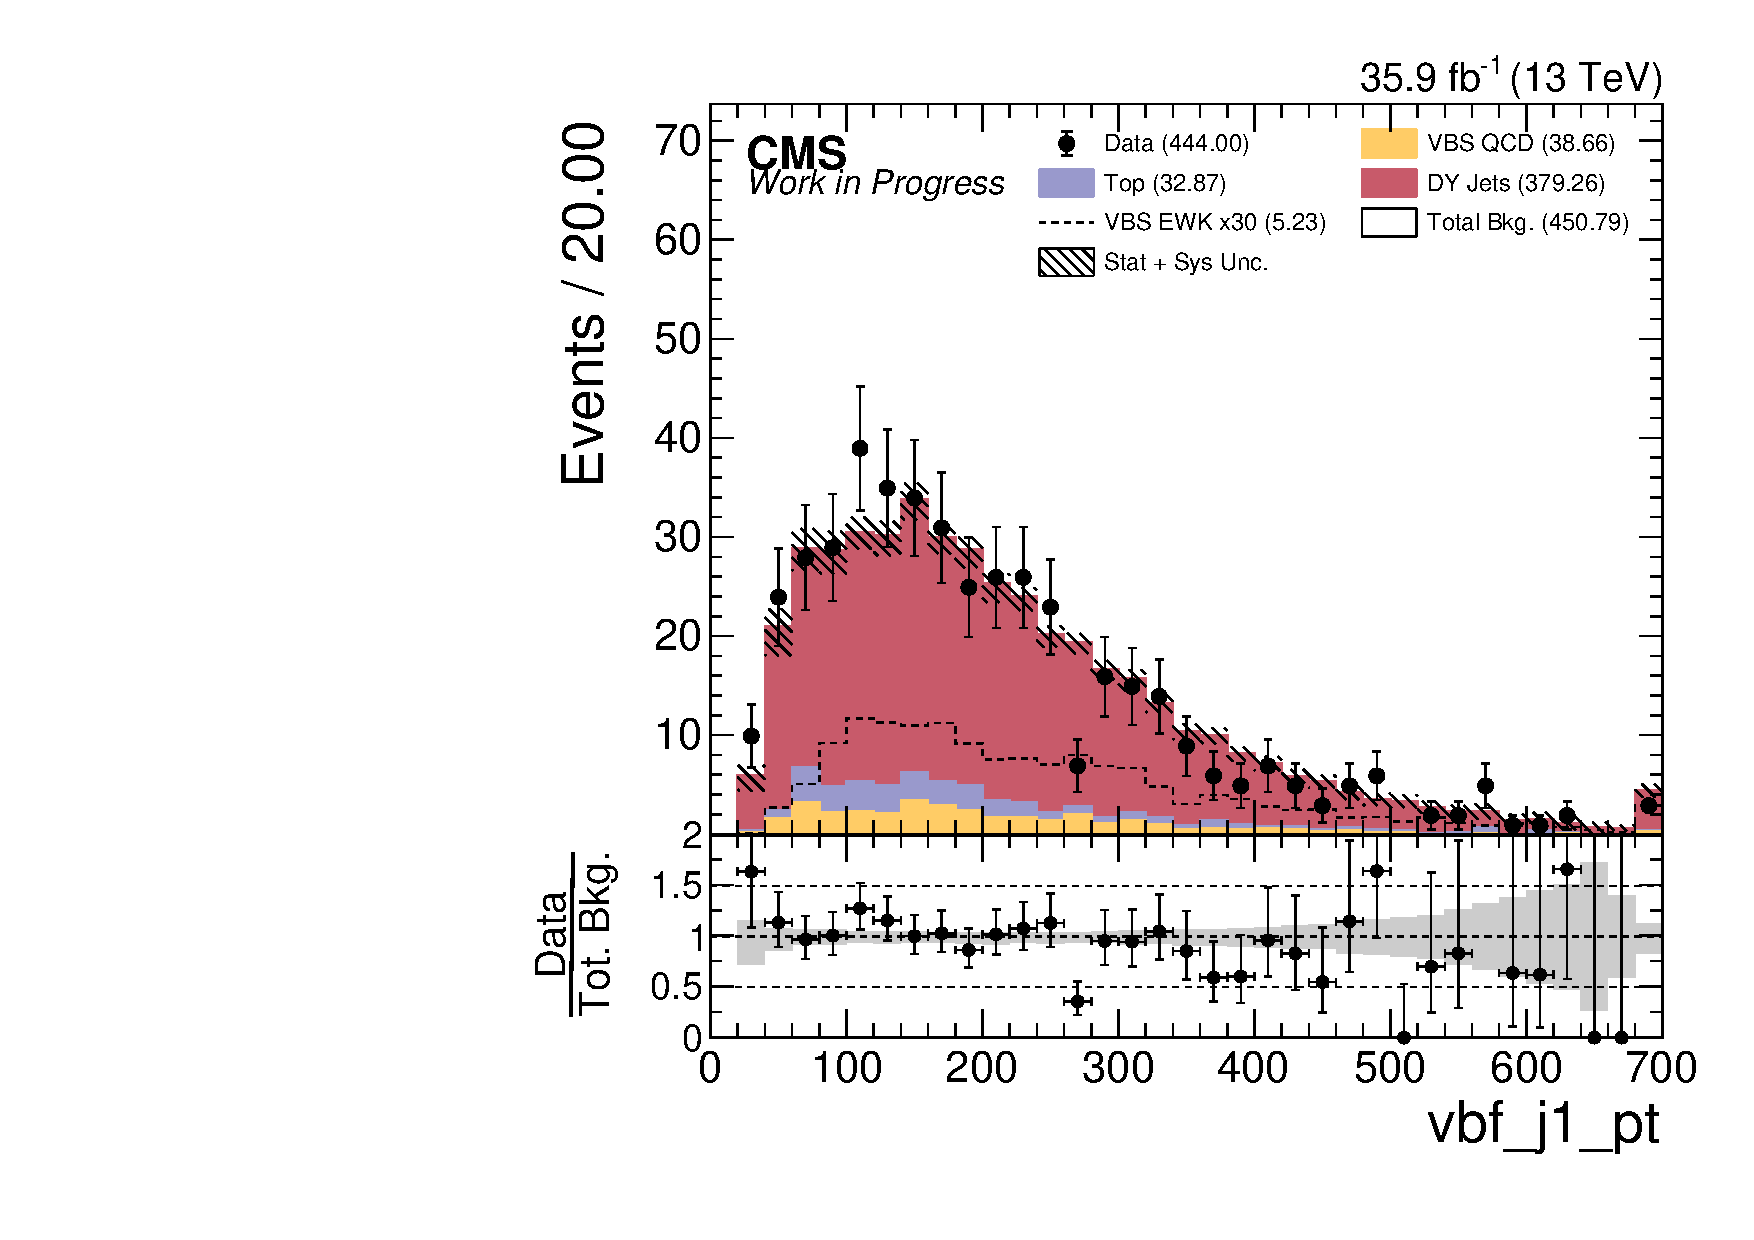
\includegraphics[width=0.335\textwidth]{analysis_plots/2016_zv/cr_vjets_l/vbf_j1_pt.pdf} \hspace{-10pt}
  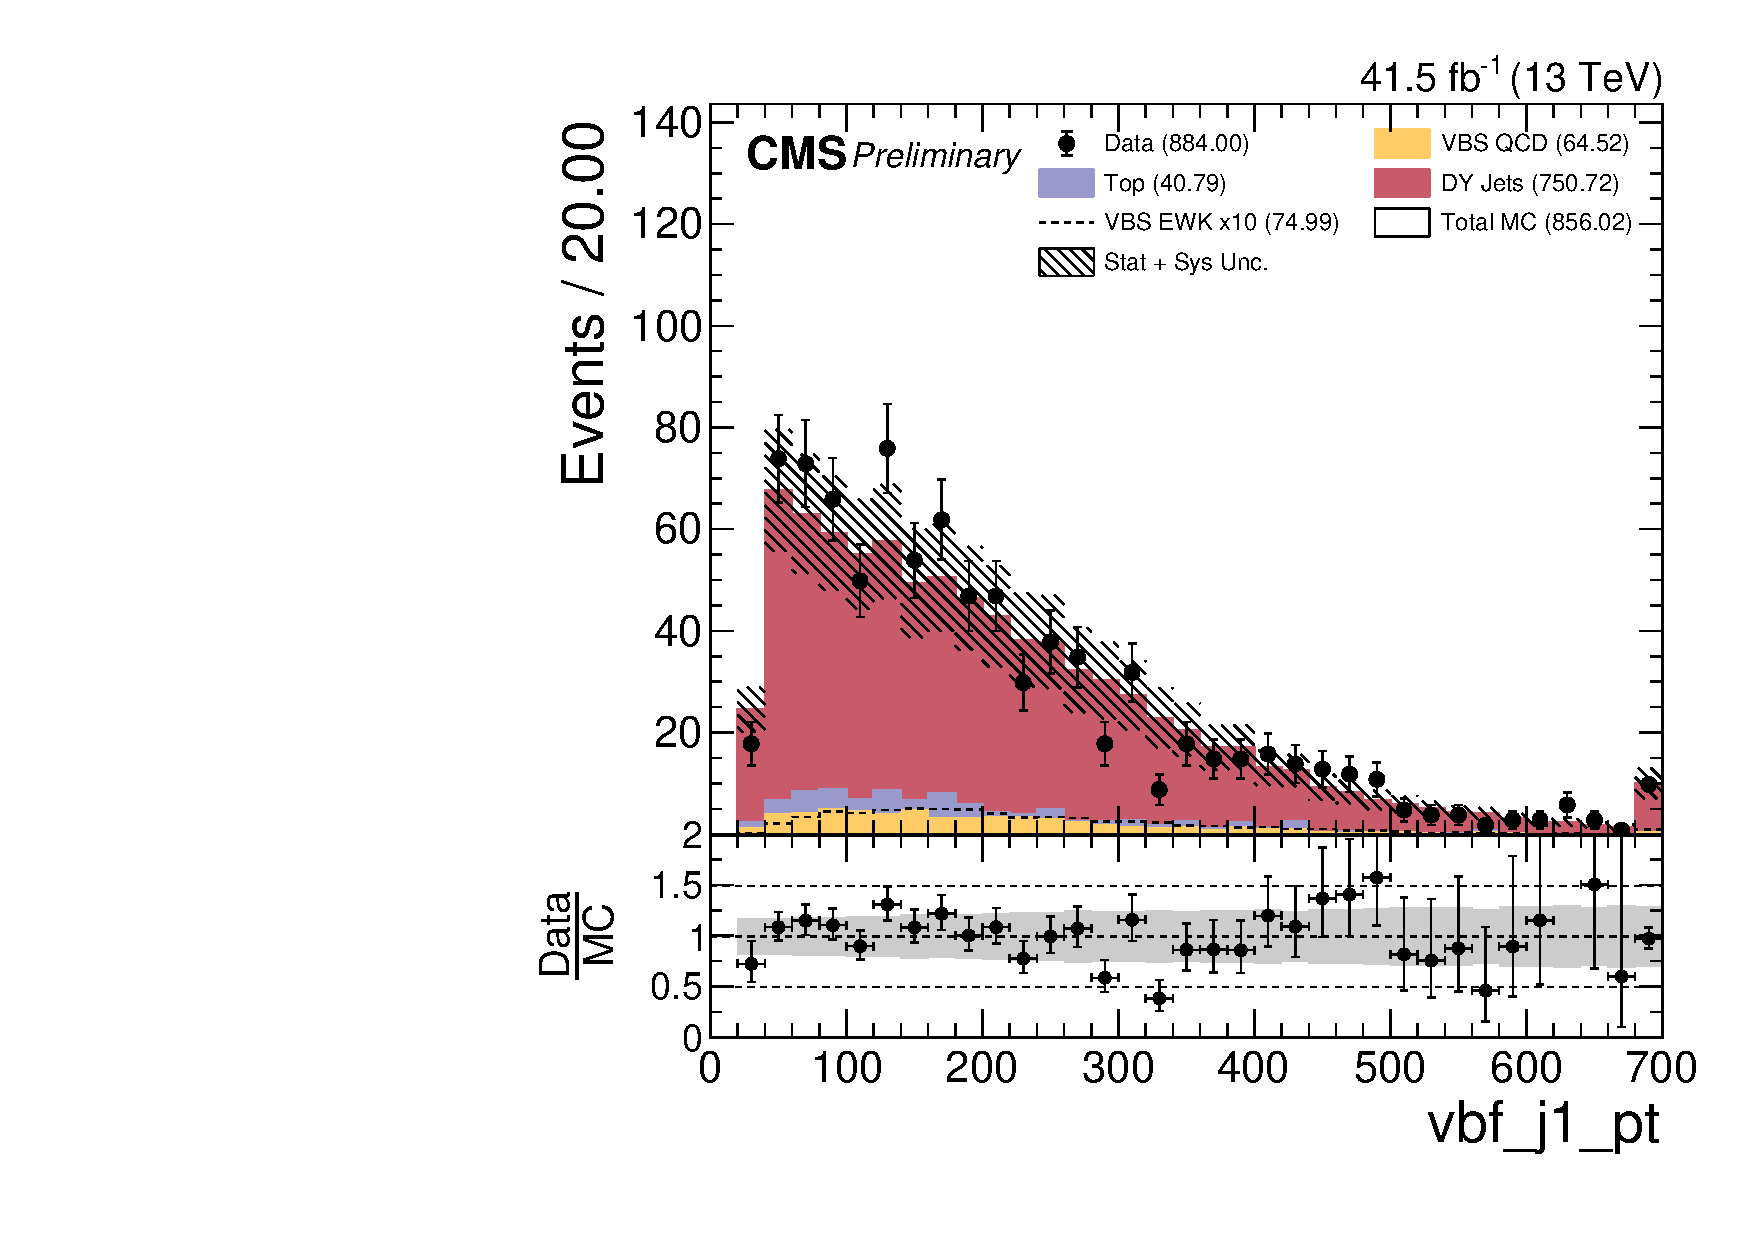
\includegraphics[width=0.335\textwidth]{analysis_plots/2017_zv/cr_vjets_l/vbf_j1_pt.pdf} \hspace{-10pt}
  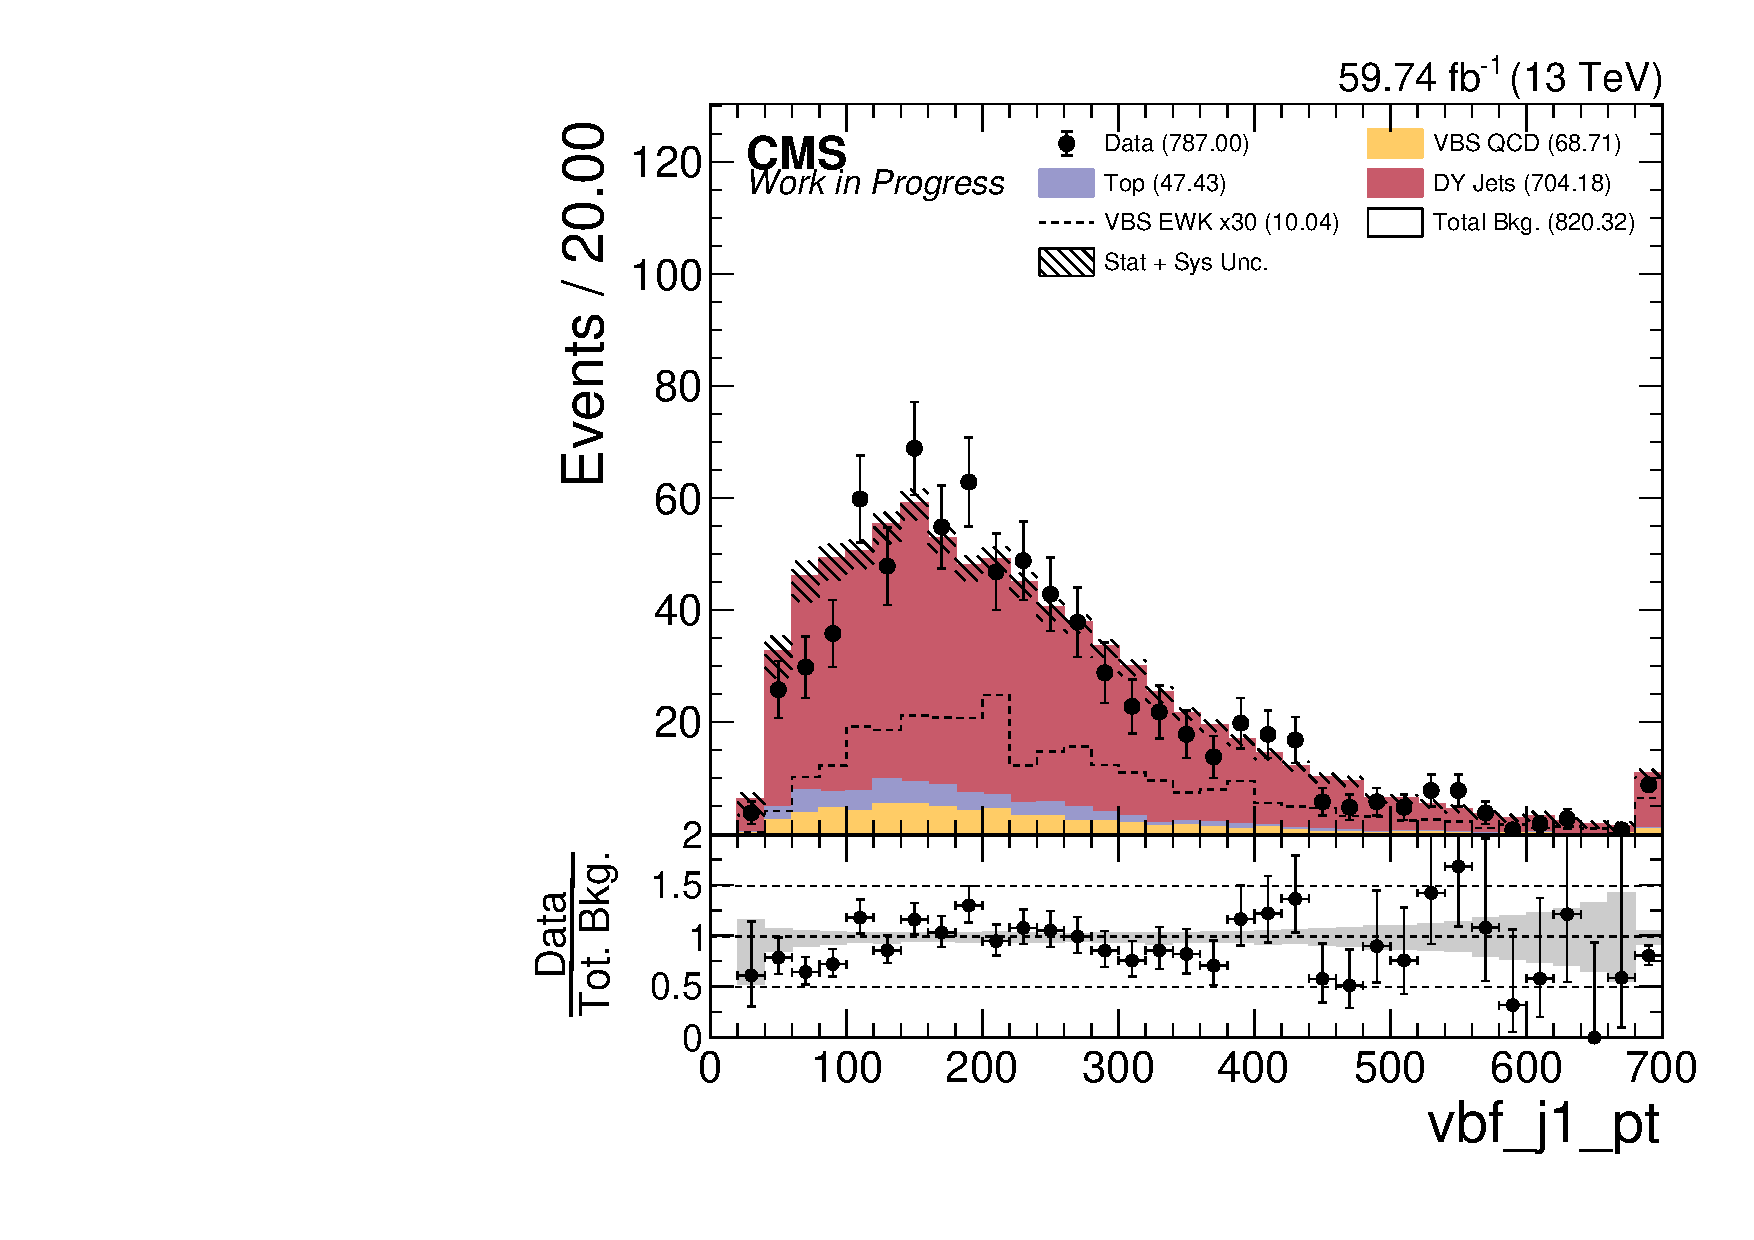
\includegraphics[width=0.335\textwidth]{analysis_plots/2018_zv/cr_vjets_l/vbf_j1_pt.pdf} \hspace{-10pt} \\
  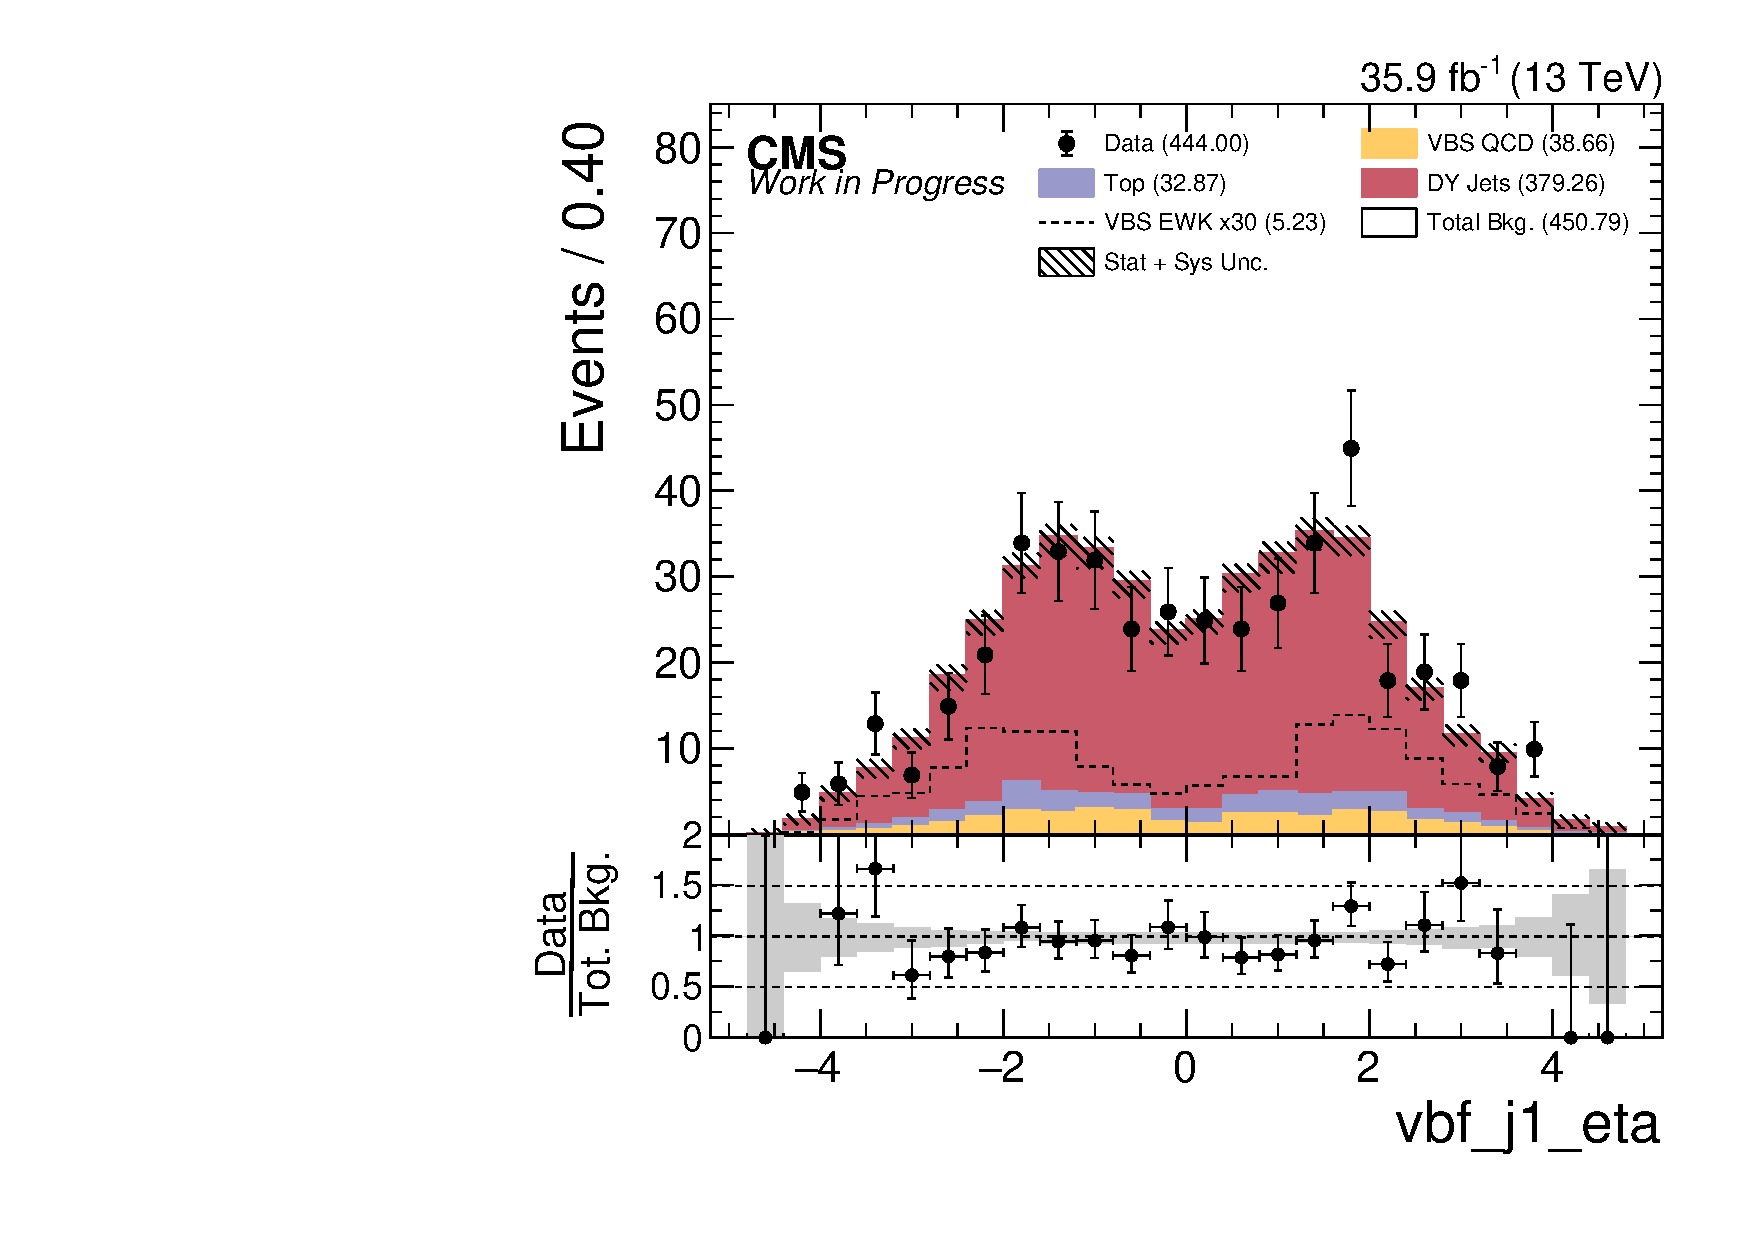
\includegraphics[width=0.335\textwidth]{analysis_plots/2016_zv/cr_vjets_l/vbf_j1_eta.pdf} \hspace{-10pt}
  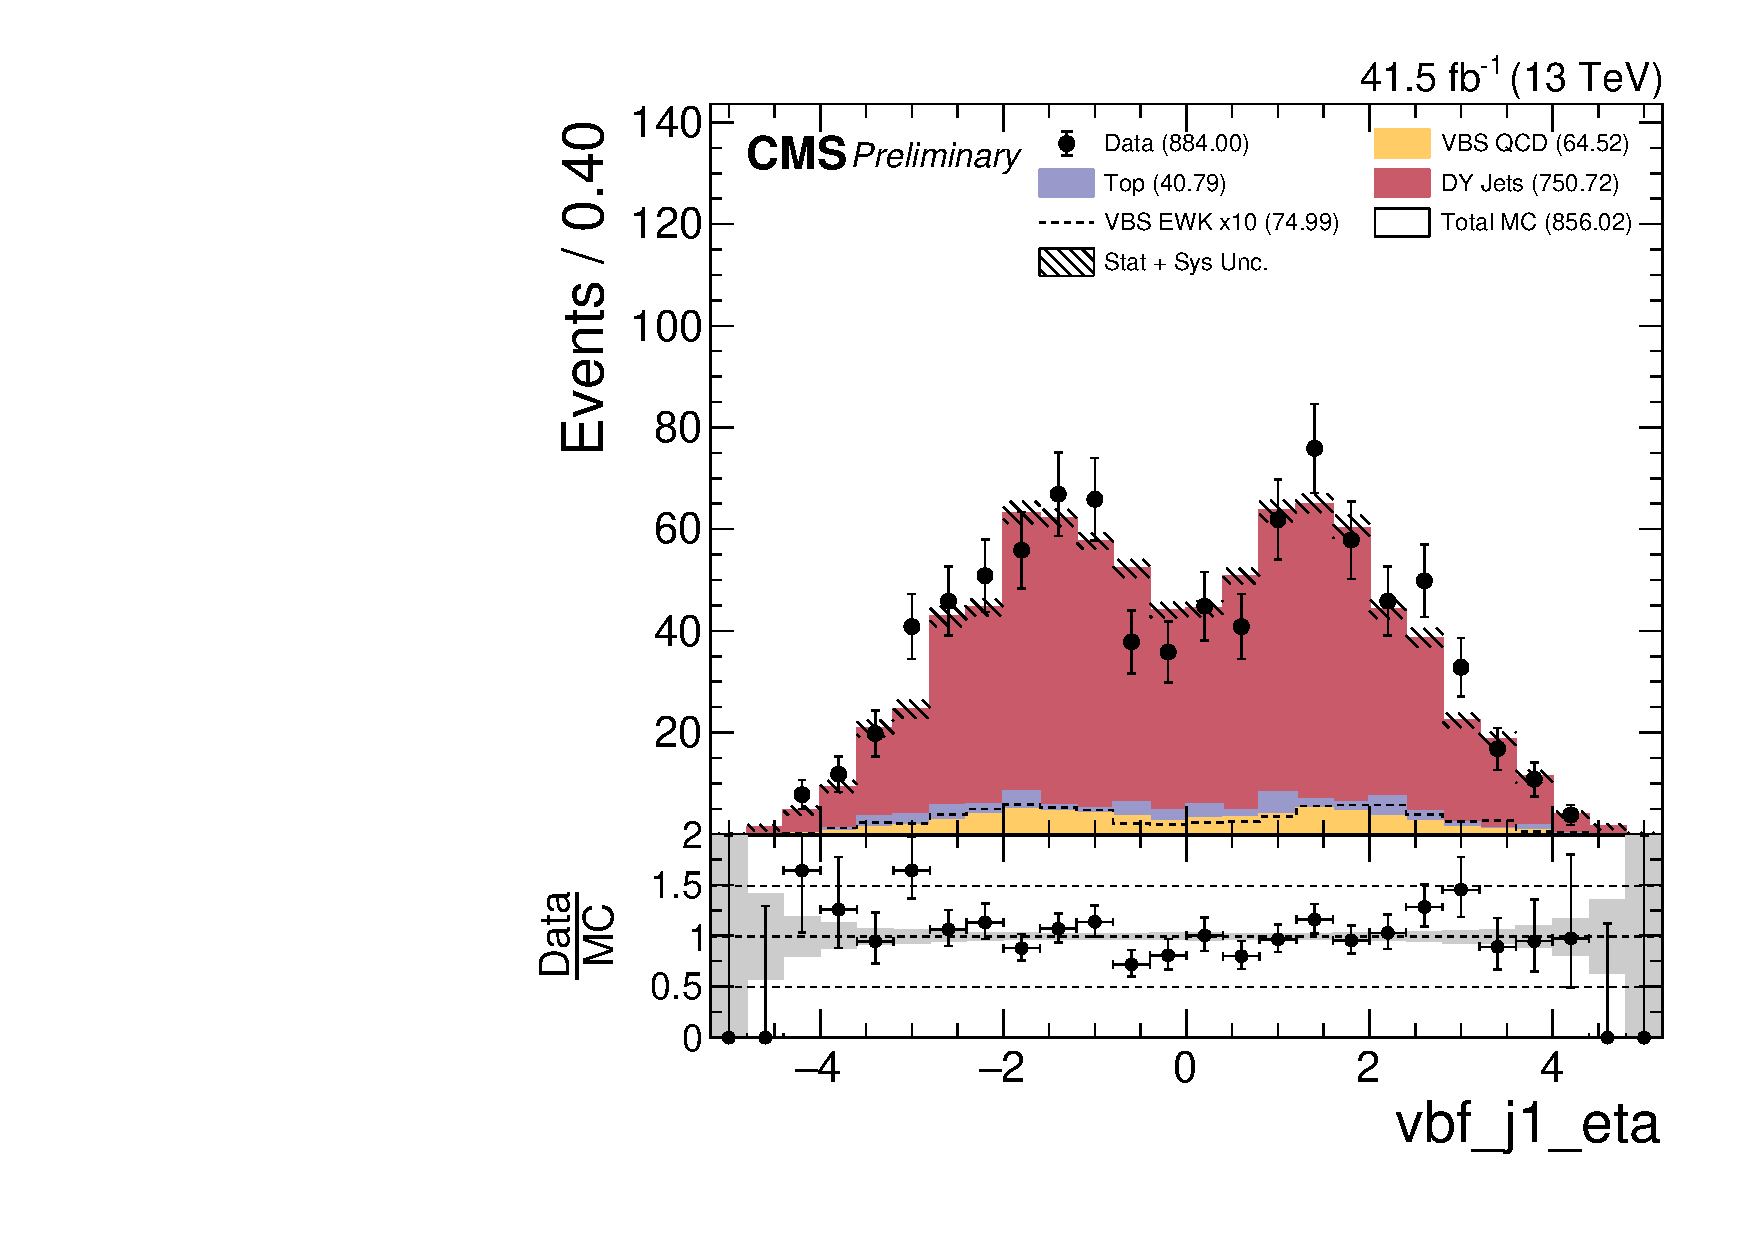
\includegraphics[width=0.335\textwidth]{analysis_plots/2017_zv/cr_vjets_l/vbf_j1_eta.pdf} \hspace{-10pt}
  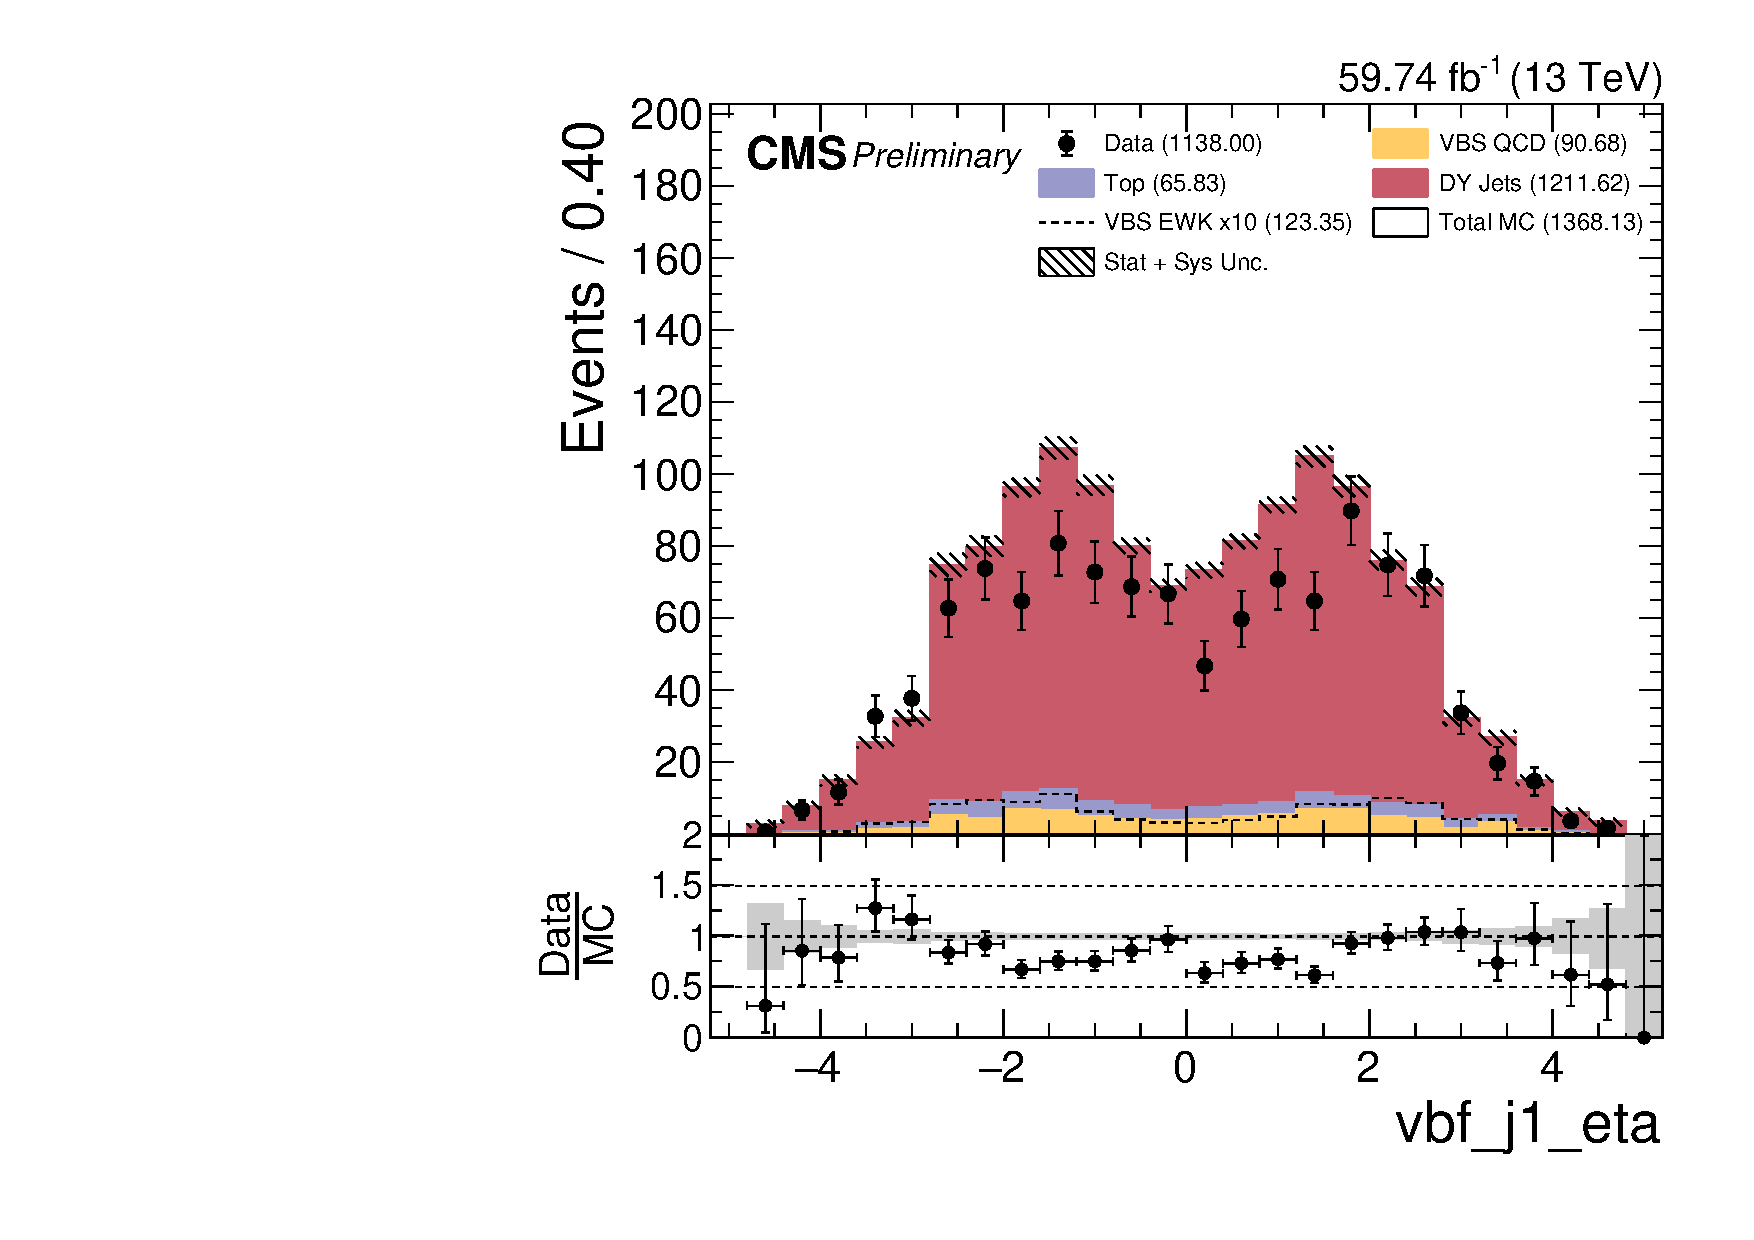
\includegraphics[width=0.335\textwidth]{analysis_plots/2018_zv/cr_vjets_l/vbf_j1_eta.pdf} \hspace{-10pt} \\
  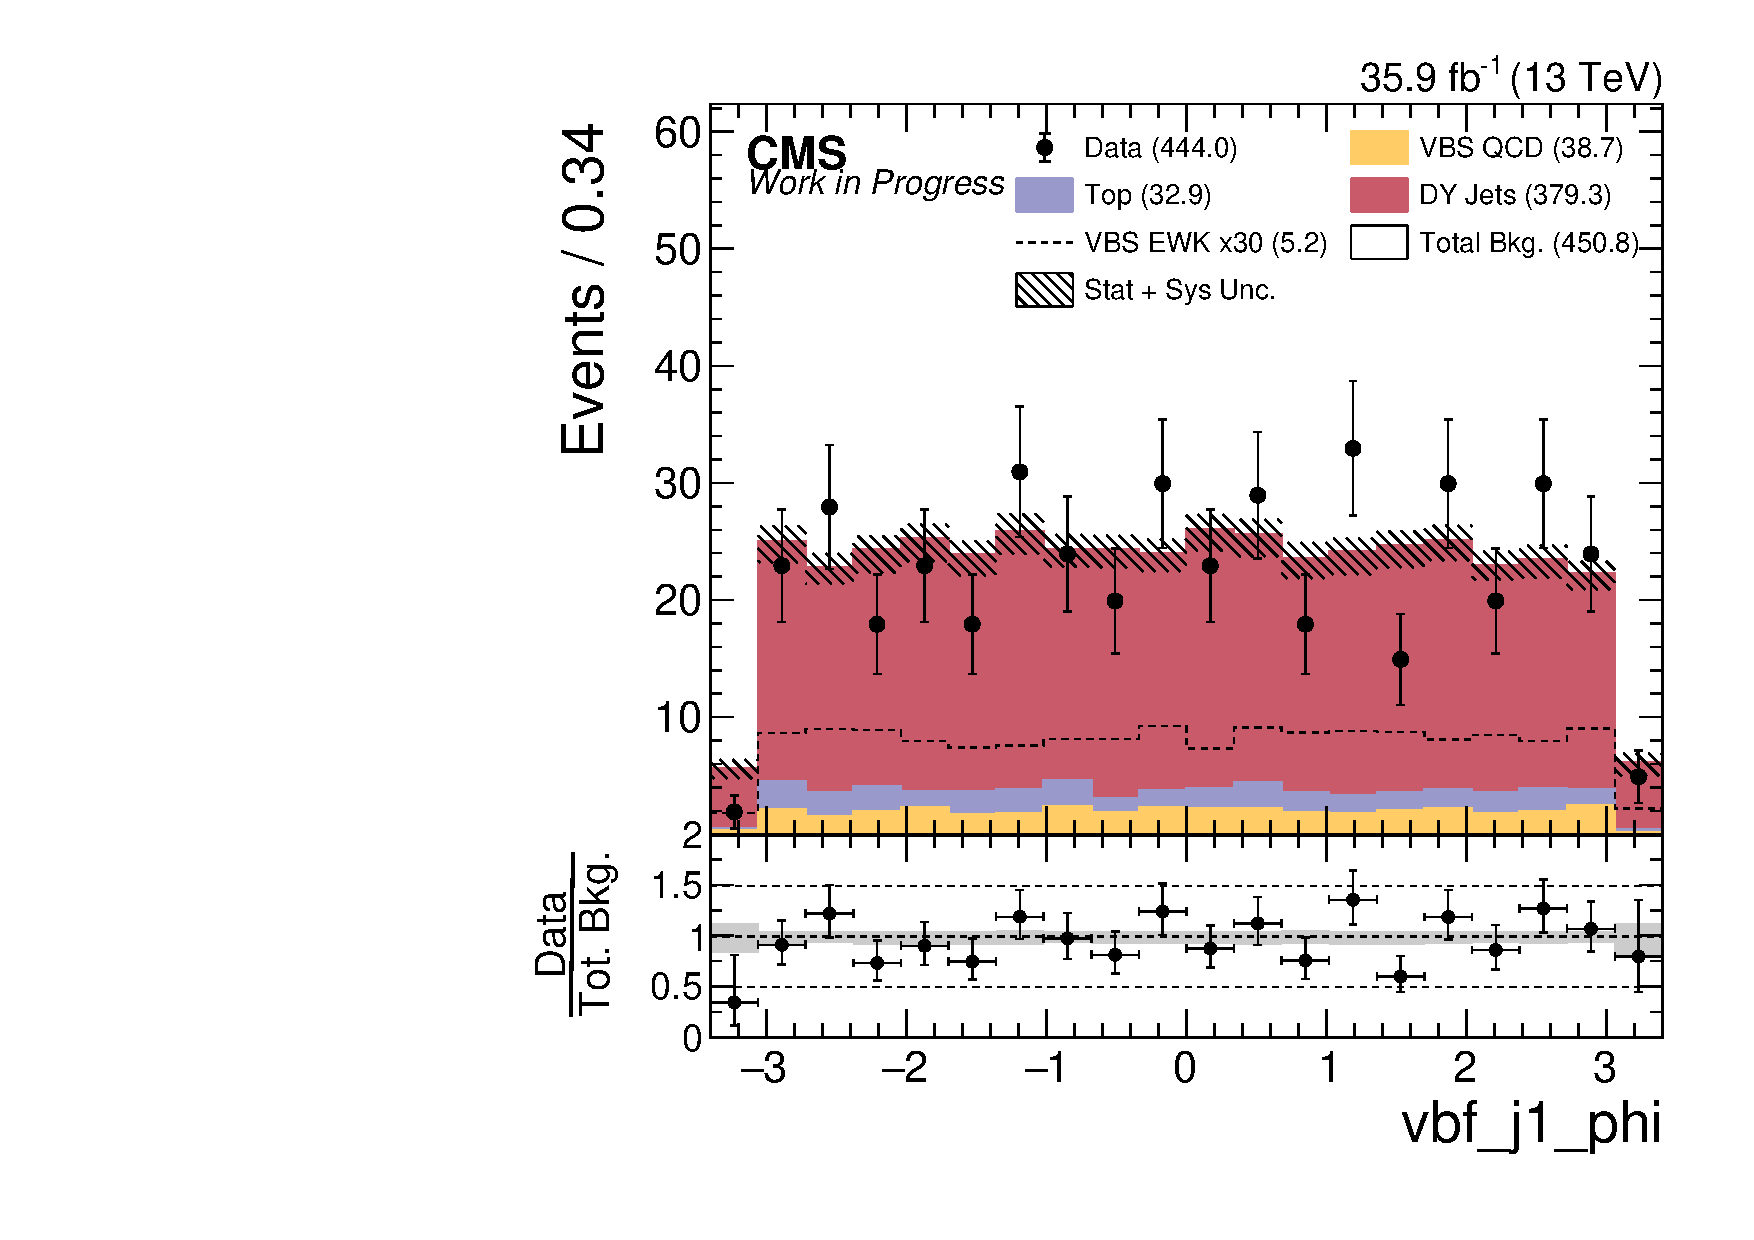
\includegraphics[width=0.335\textwidth]{analysis_plots/2016_zv/cr_vjets_l/vbf_j1_phi.pdf} \hspace{-10pt}
  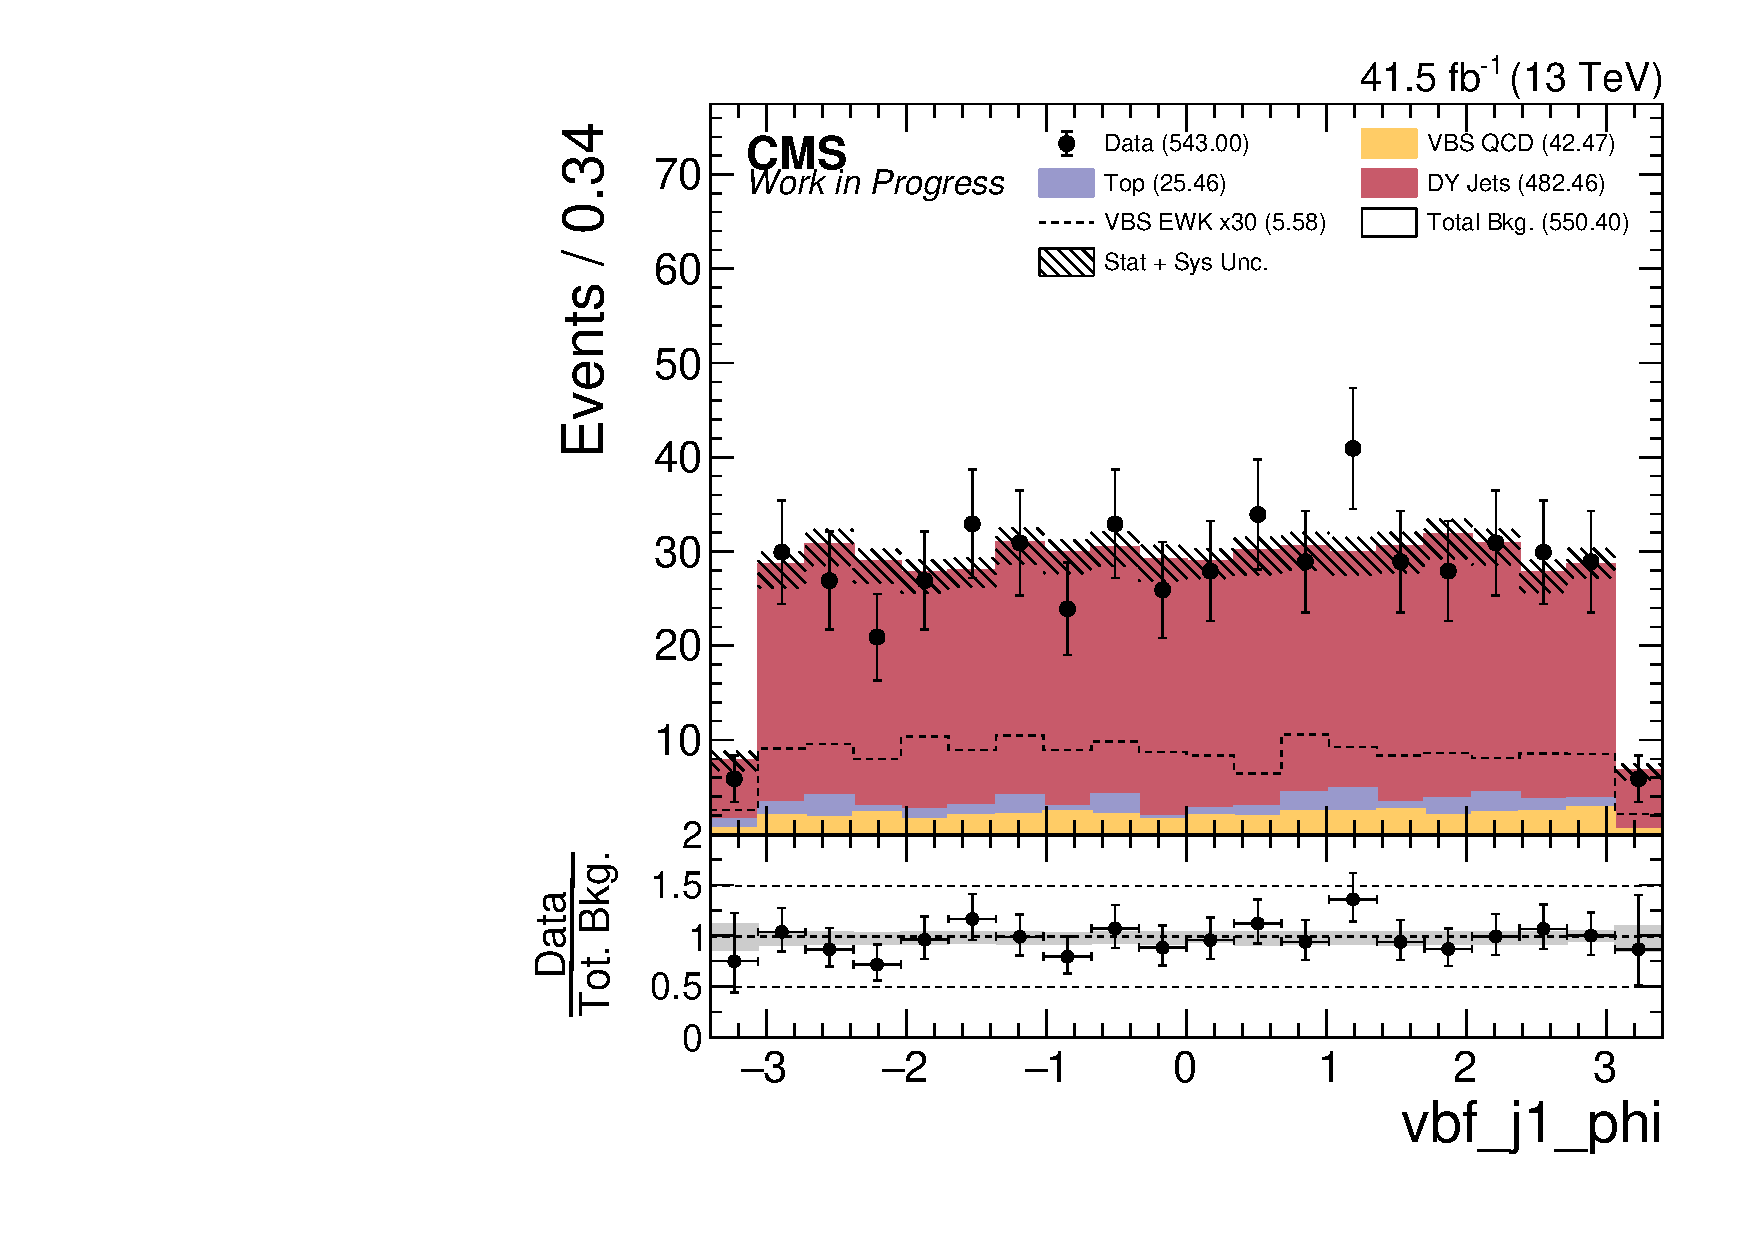
\includegraphics[width=0.335\textwidth]{analysis_plots/2017_zv/cr_vjets_l/vbf_j1_phi.pdf} \hspace{-10pt}
  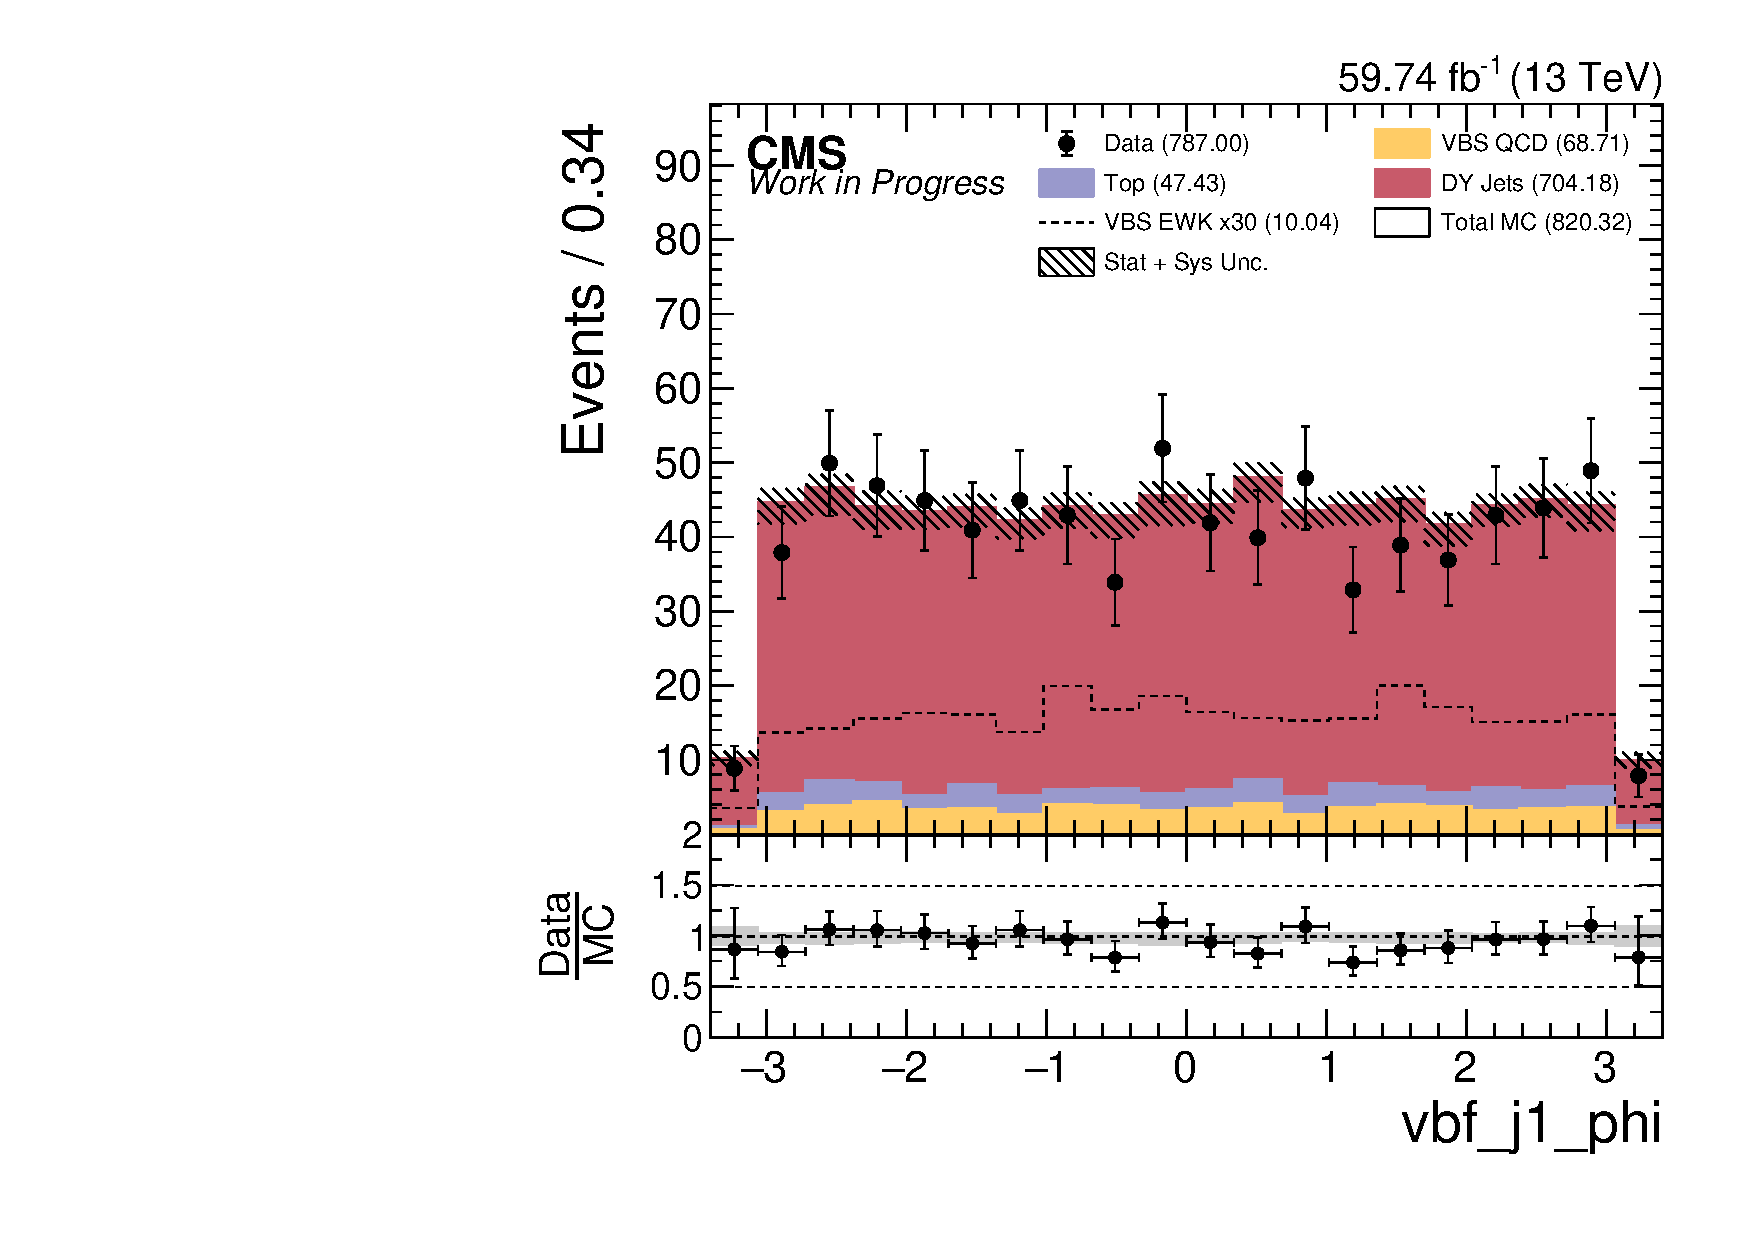
\includegraphics[width=0.335\textwidth]{analysis_plots/2018_zv/cr_vjets_l/vbf_j1_phi.pdf} \hspace{-10pt} \\
  \caption[DY+Jets Control Region: Leading VBS tagged jet kinematics in Boosted ZV Channel]%
  {DY+Jets Control Region: Leading VBS tagged jet kinematics in Boosted ZV Channel.
    Error bars include statistical uncertainty on total background,
    JES and QCD scale systematic on DY+Jets and VBS\_QCD MC\@. From Left to Right: 2016,
    2017, and 2018. From Top to Bottom: \( p_T \), \( \eta \), and \( \phi \).}%
  \label{fig:zv-cr-vjets-l-vbs1-pt-eta-m}
\end{figure}

\begin{figure}[!ht]
  \centering
  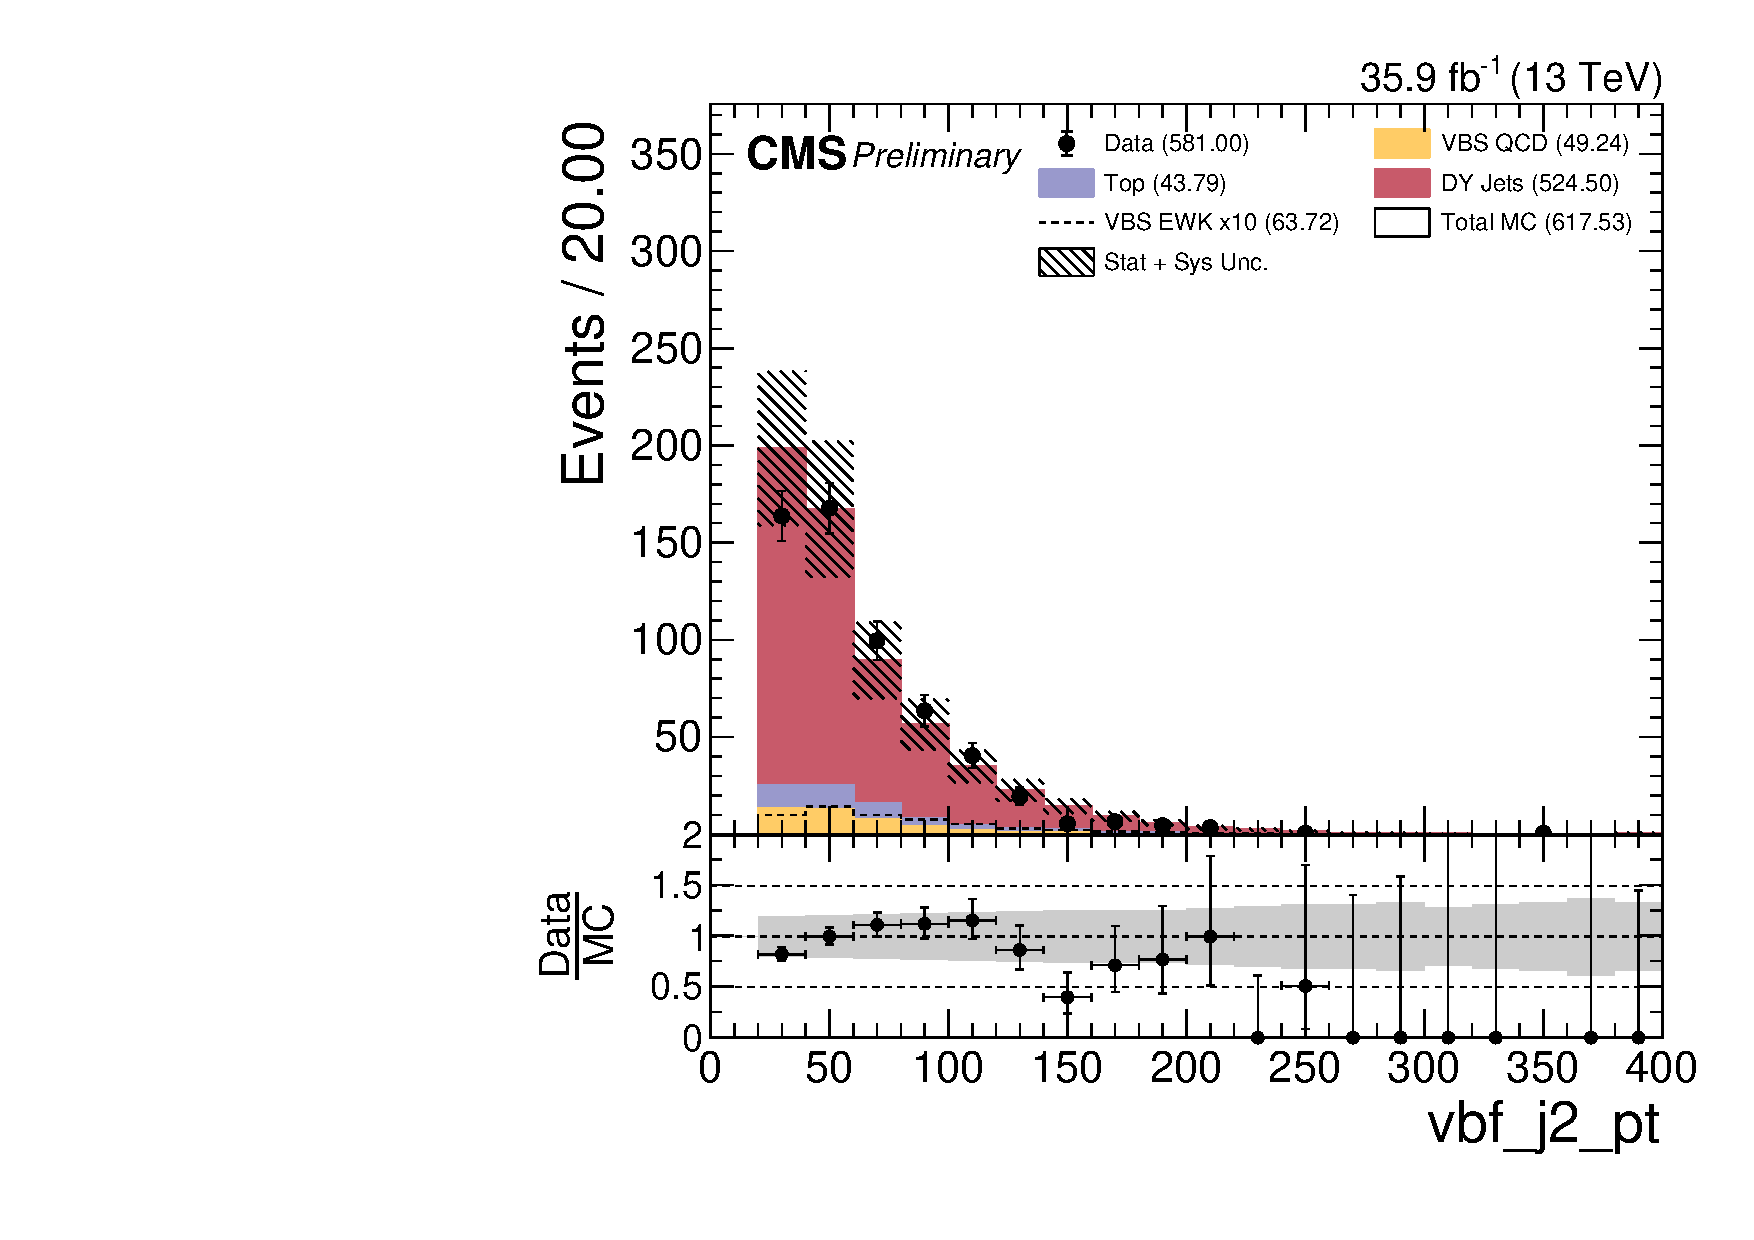
\includegraphics[width=0.335\textwidth]{analysis_plots/2016_zv/cr_vjets_l/vbf_j2_pt.pdf} \hspace{-10pt}
  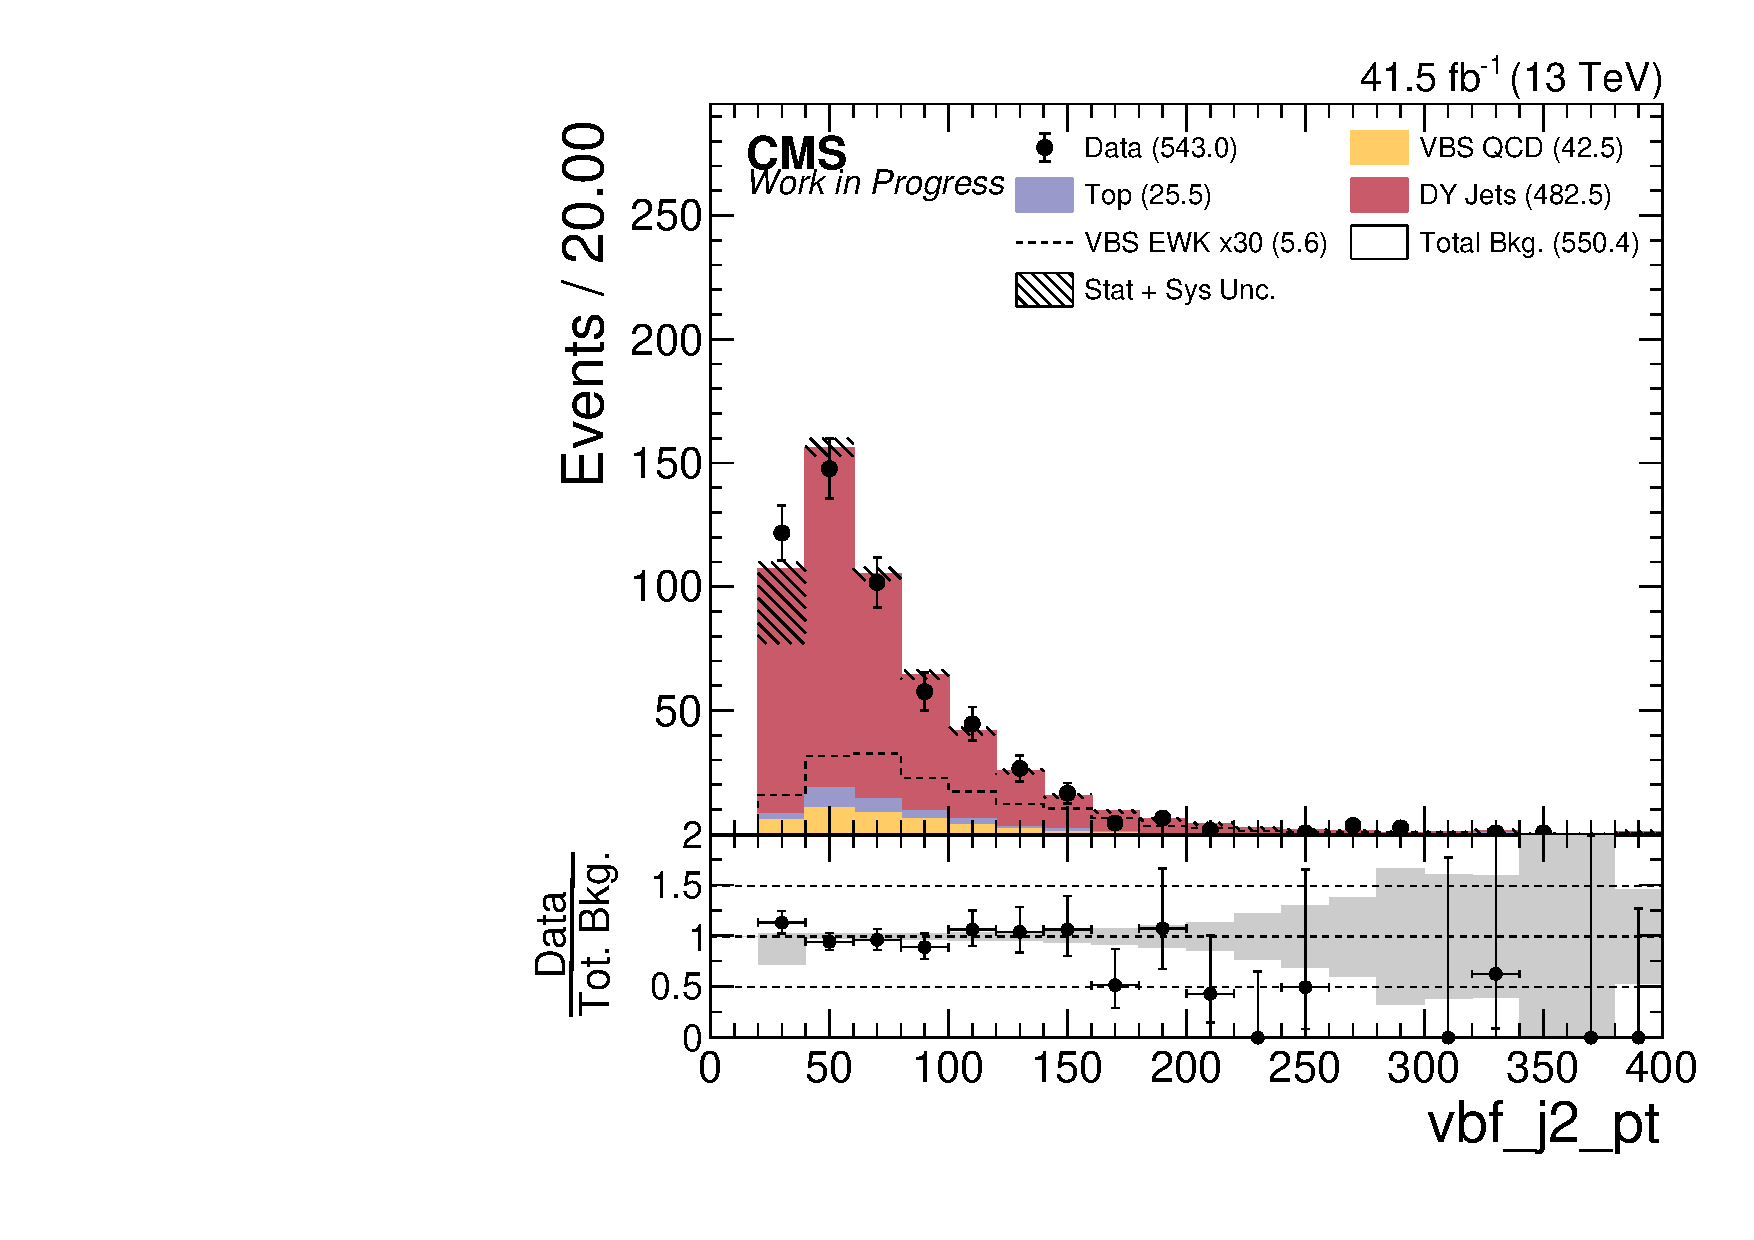
\includegraphics[width=0.335\textwidth]{analysis_plots/2017_zv/cr_vjets_l/vbf_j2_pt.pdf} \hspace{-10pt}
  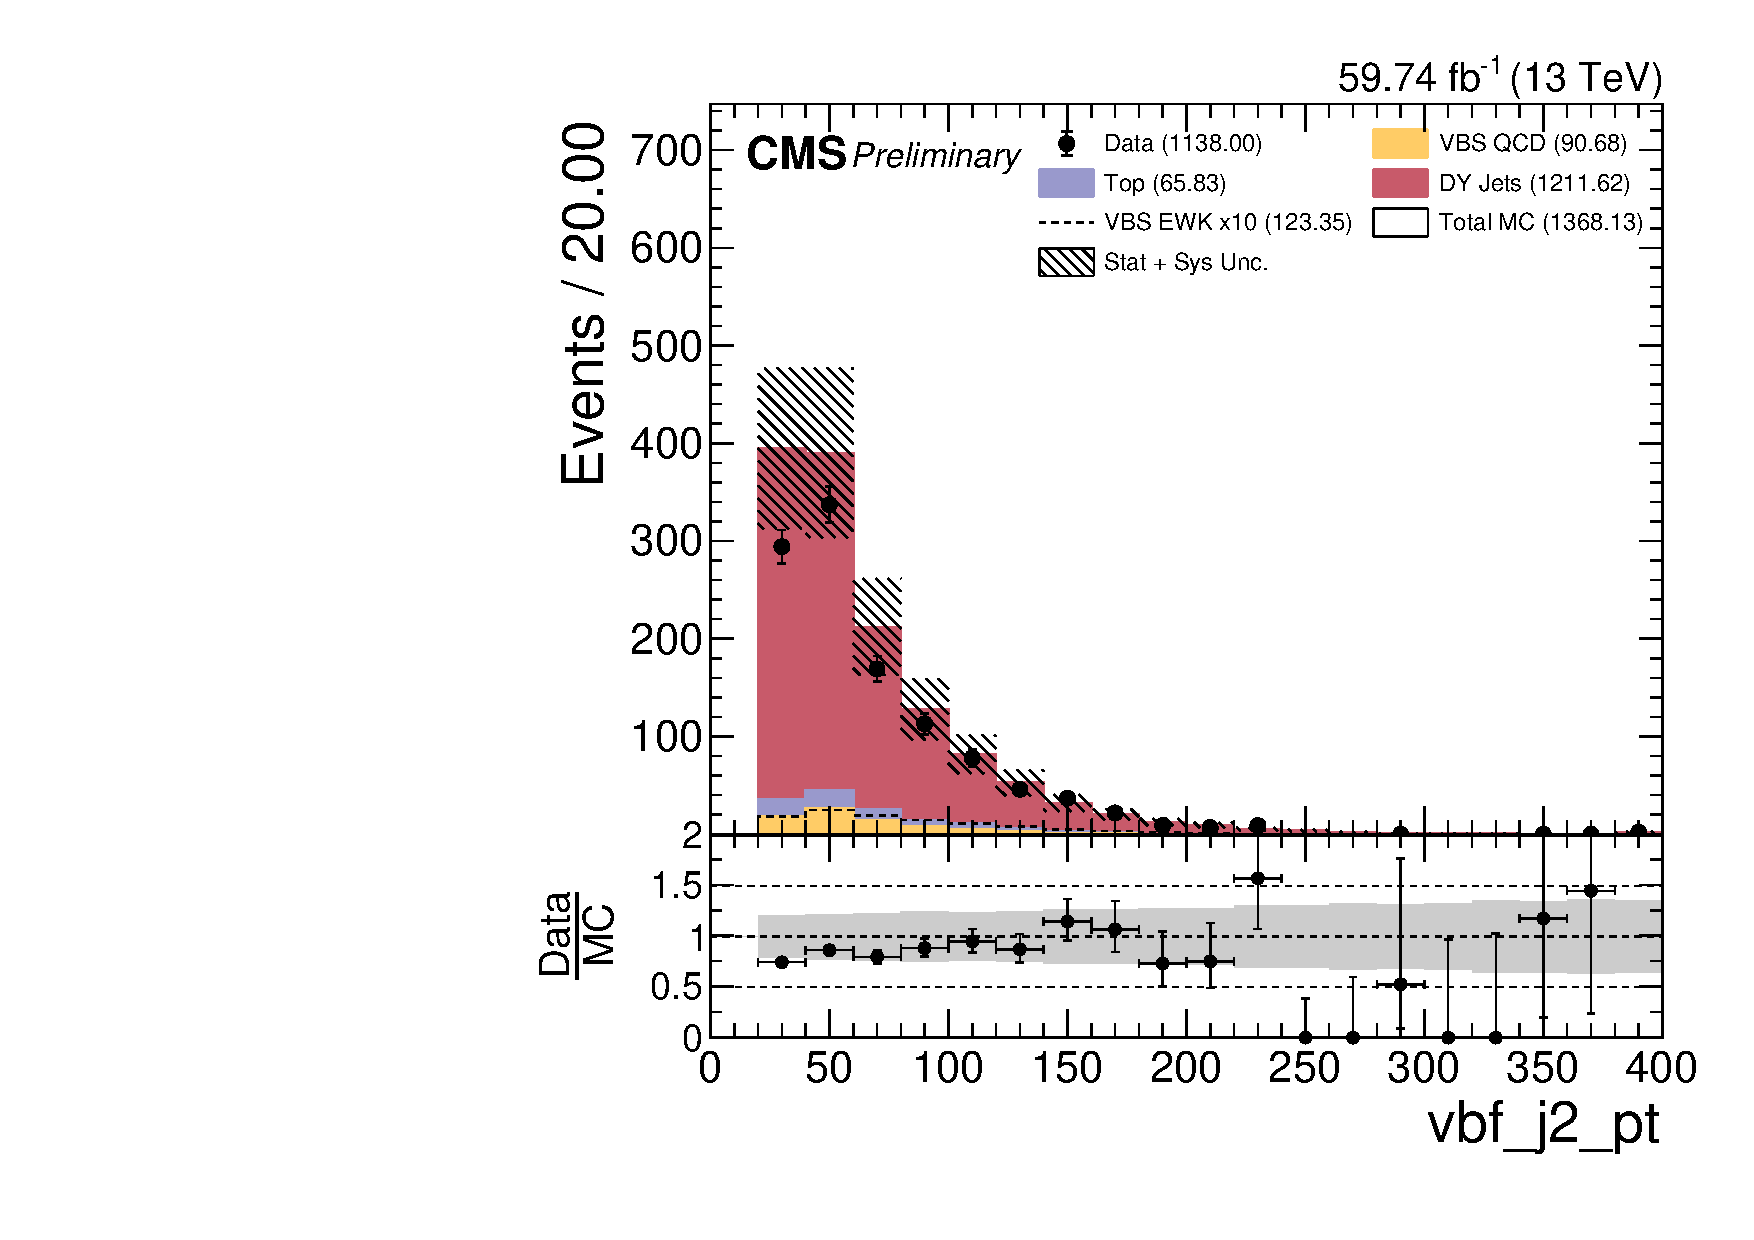
\includegraphics[width=0.335\textwidth]{analysis_plots/2018_zv/cr_vjets_l/vbf_j2_pt.pdf} \hspace{-10pt} \\
  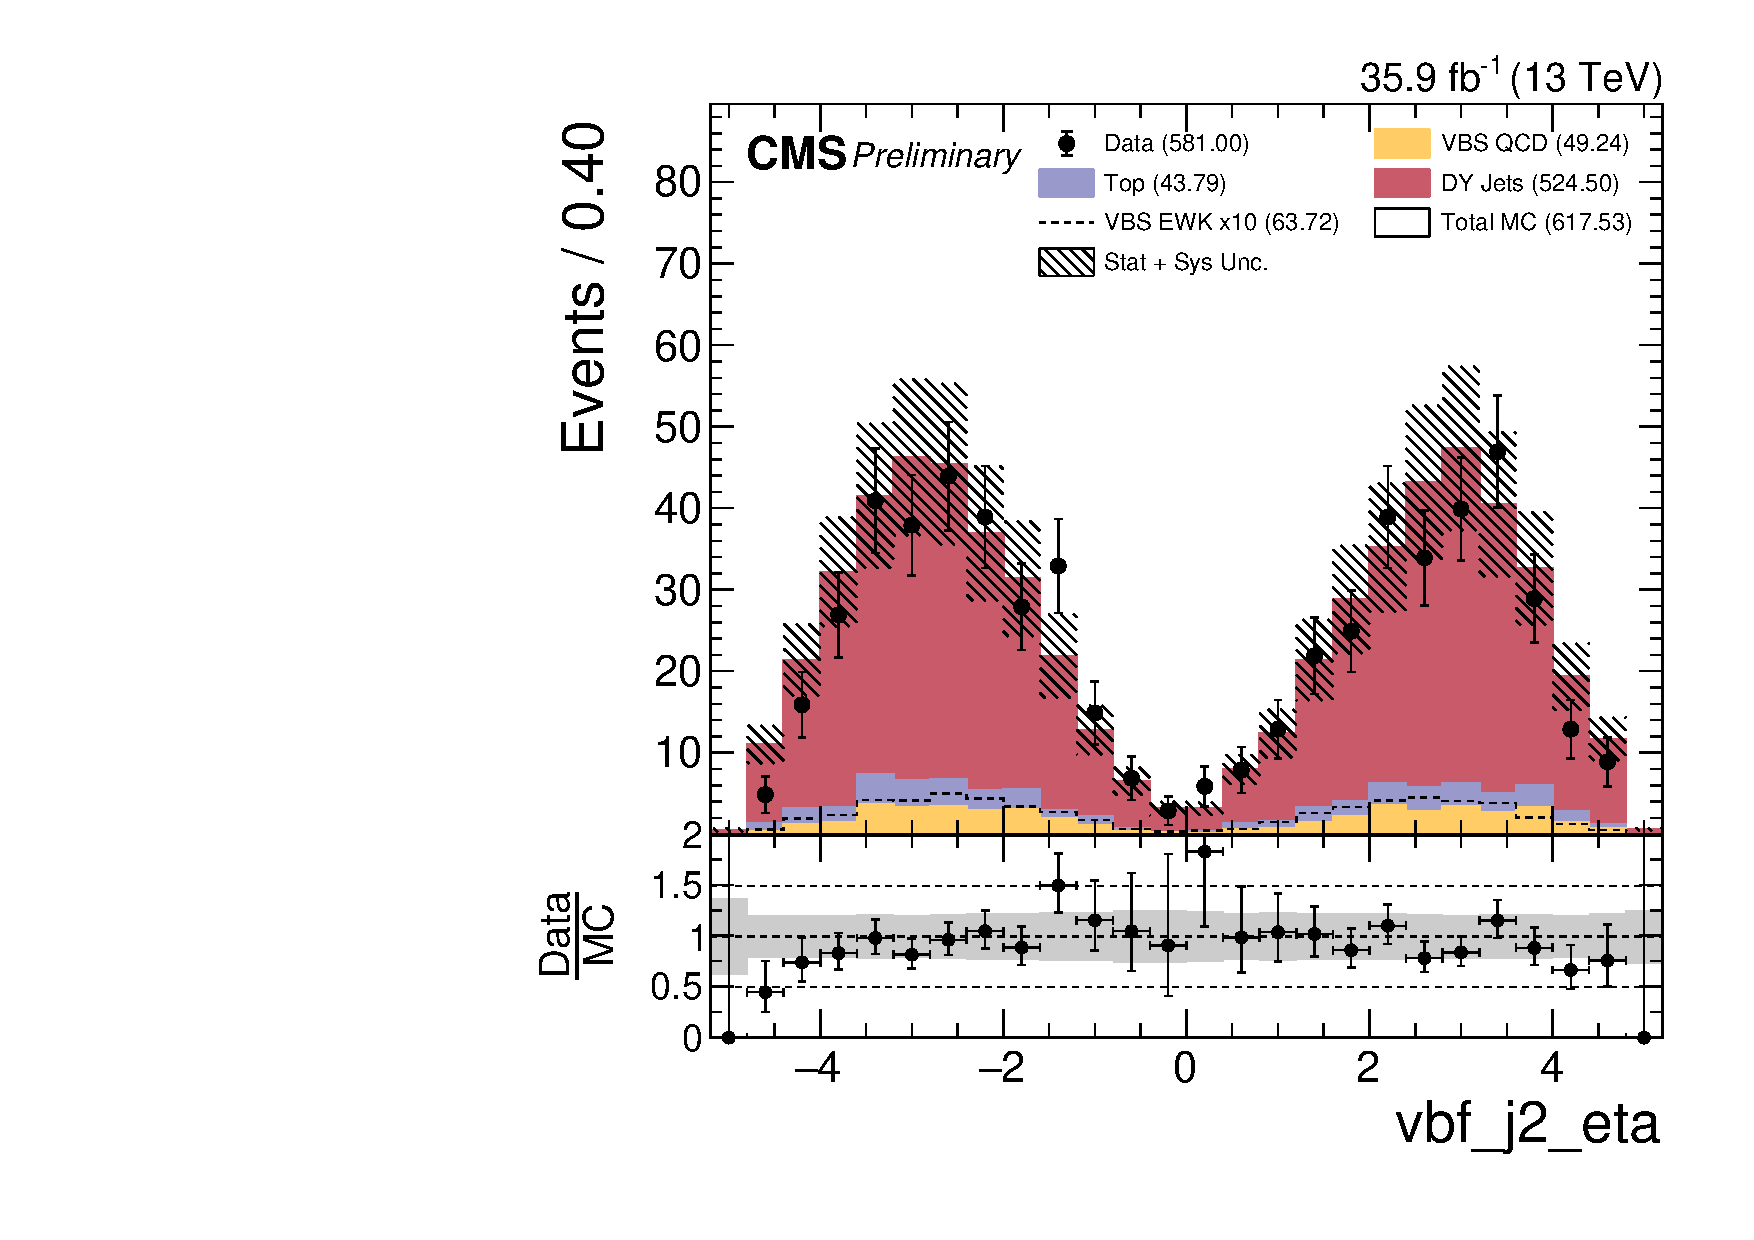
\includegraphics[width=0.335\textwidth]{analysis_plots/2016_zv/cr_vjets_l/vbf_j2_eta.pdf} \hspace{-10pt}
  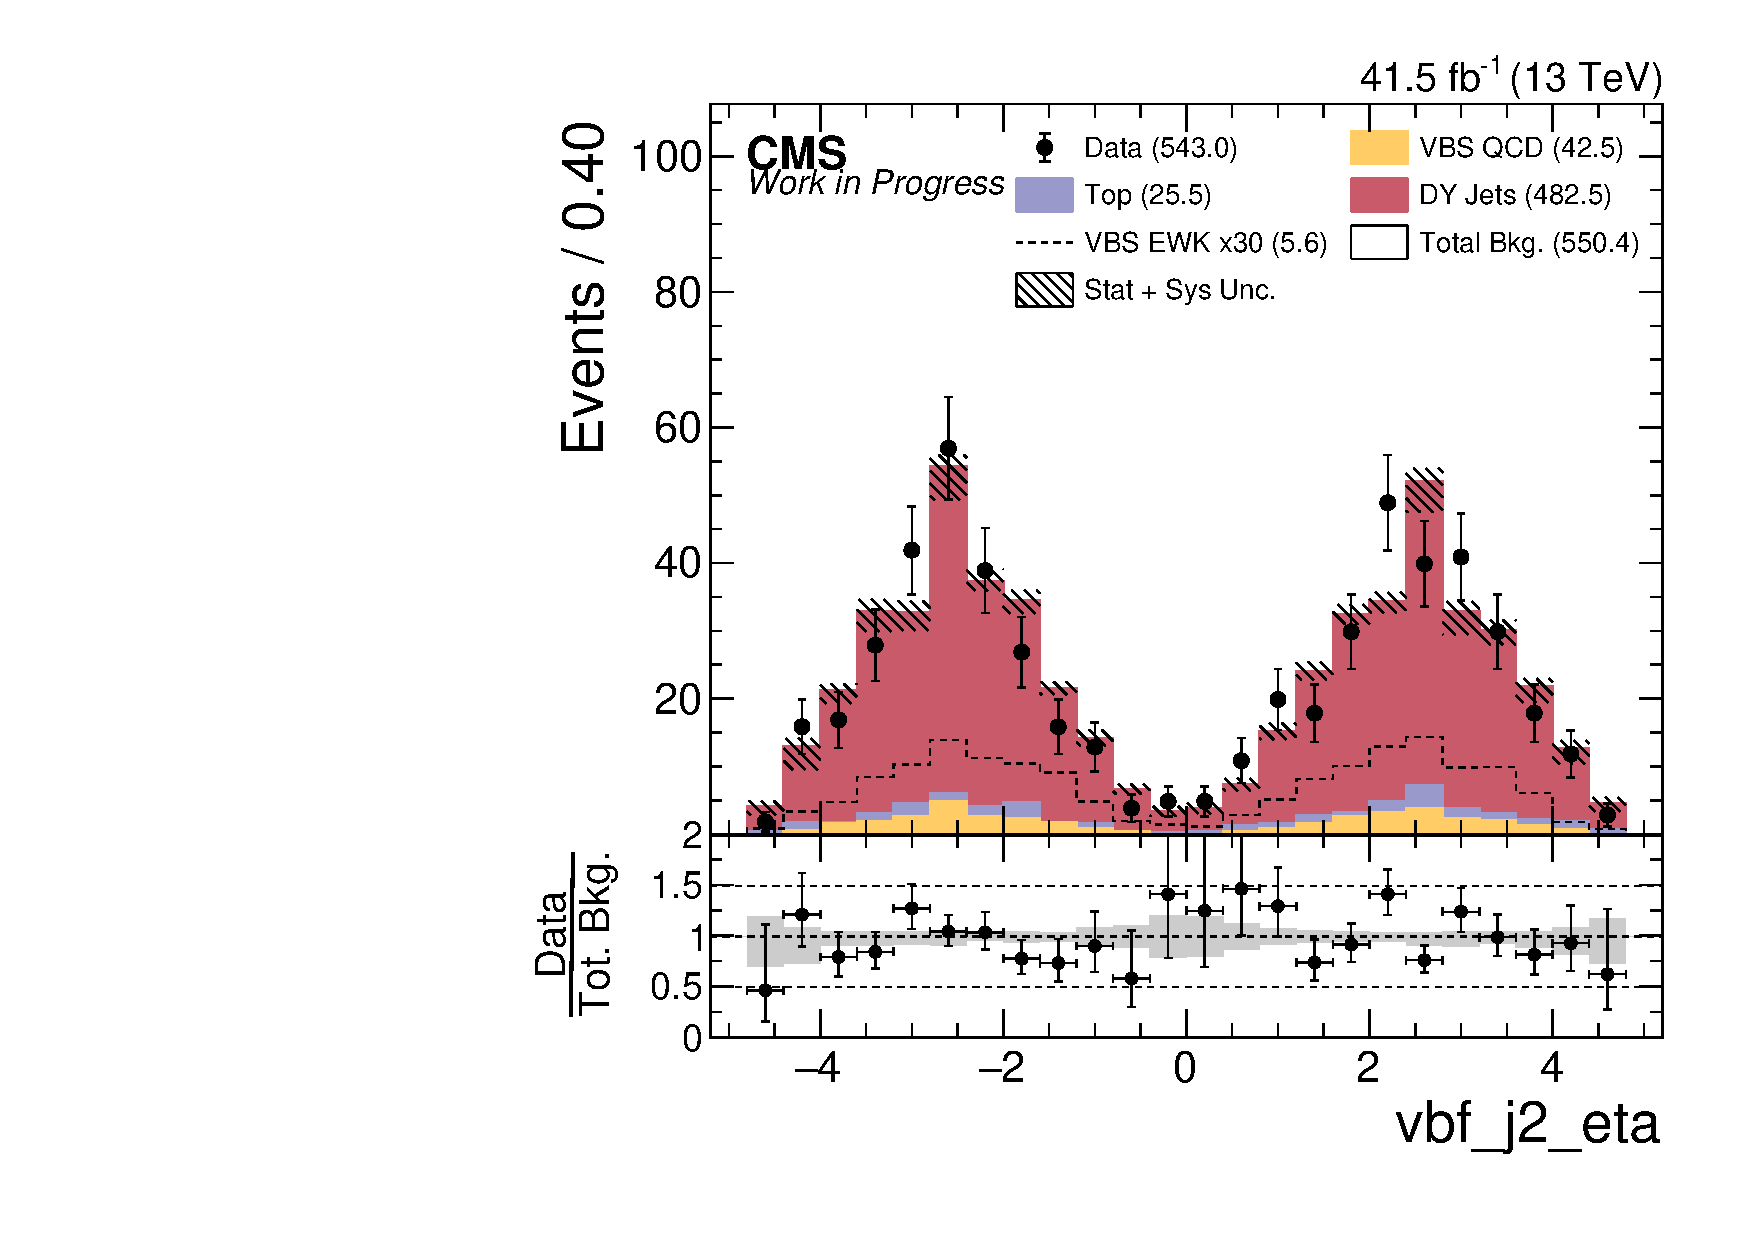
\includegraphics[width=0.335\textwidth]{analysis_plots/2017_zv/cr_vjets_l/vbf_j2_eta.pdf} \hspace{-10pt}
  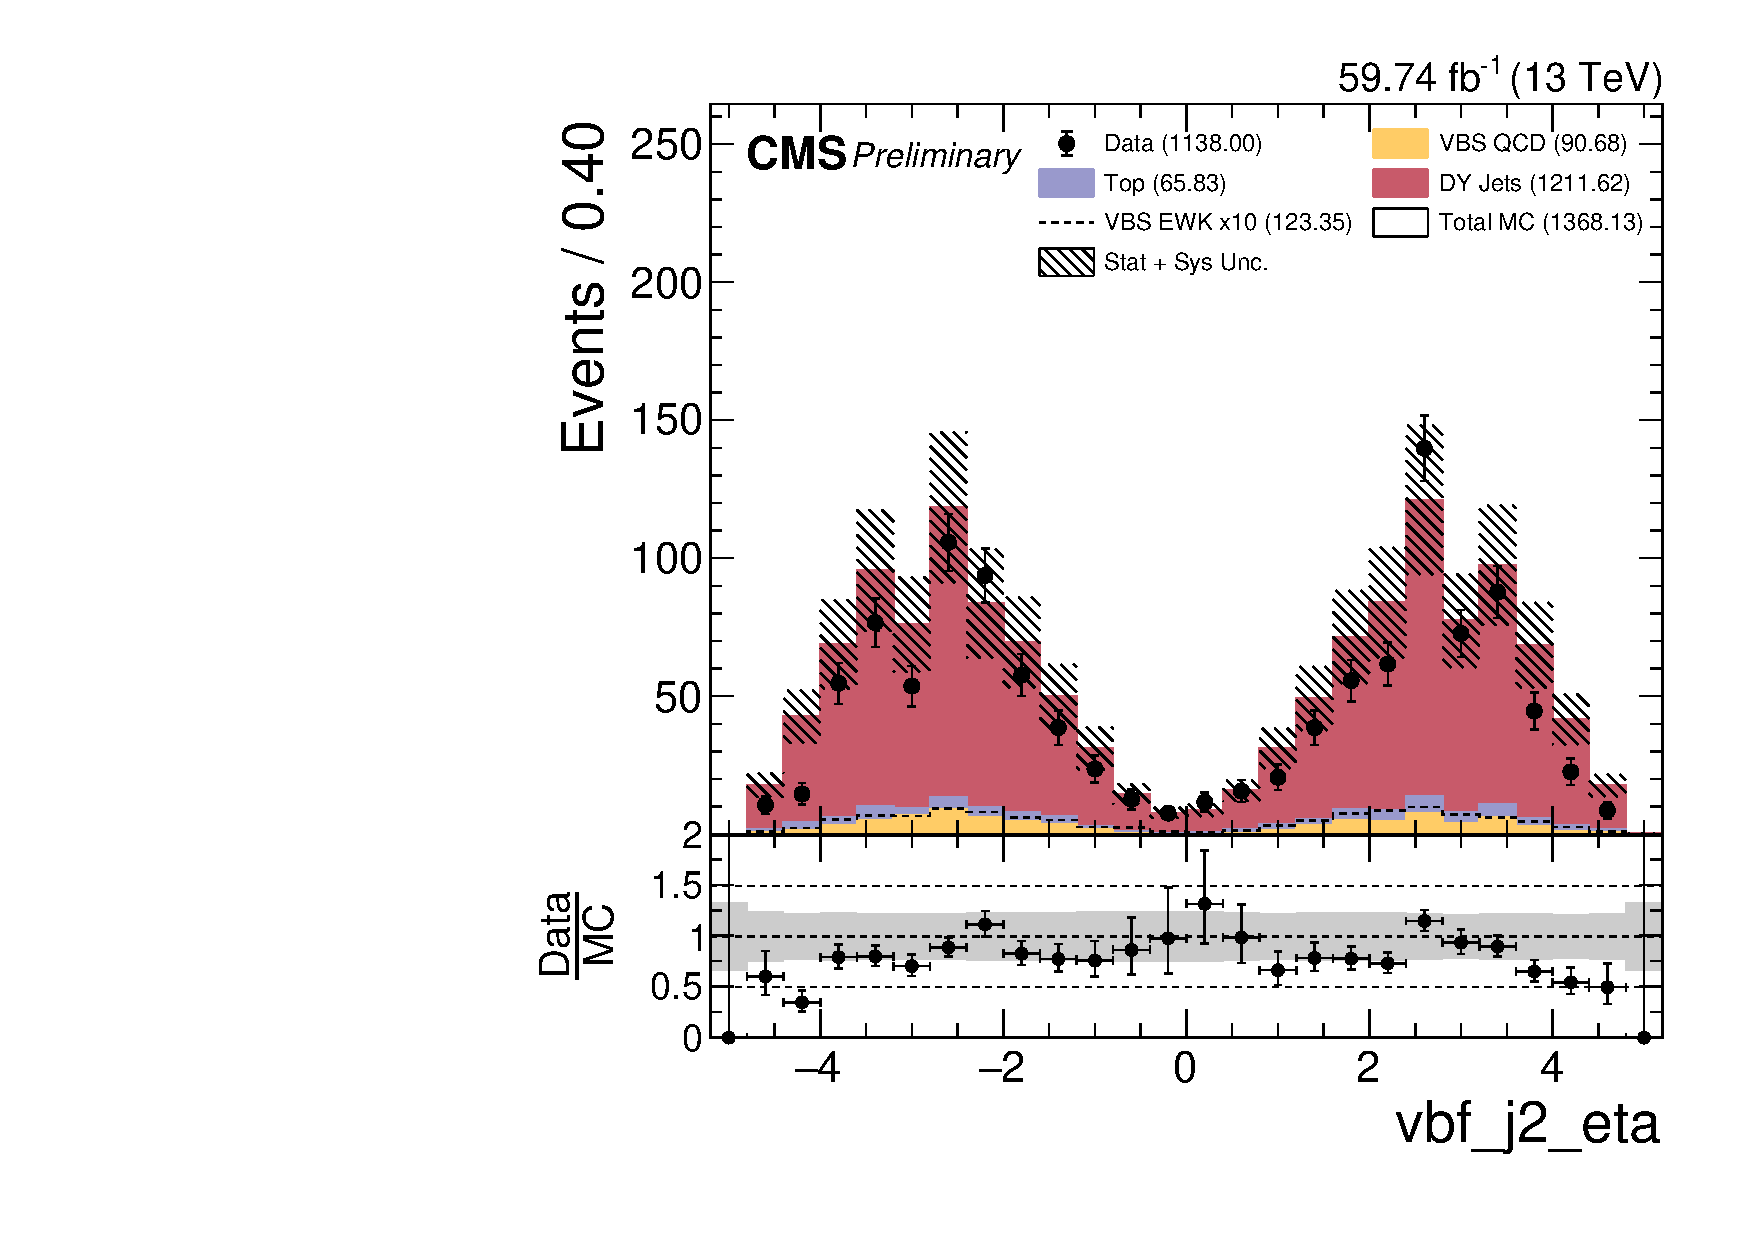
\includegraphics[width=0.335\textwidth]{analysis_plots/2018_zv/cr_vjets_l/vbf_j2_eta.pdf} \hspace{-10pt} \\
  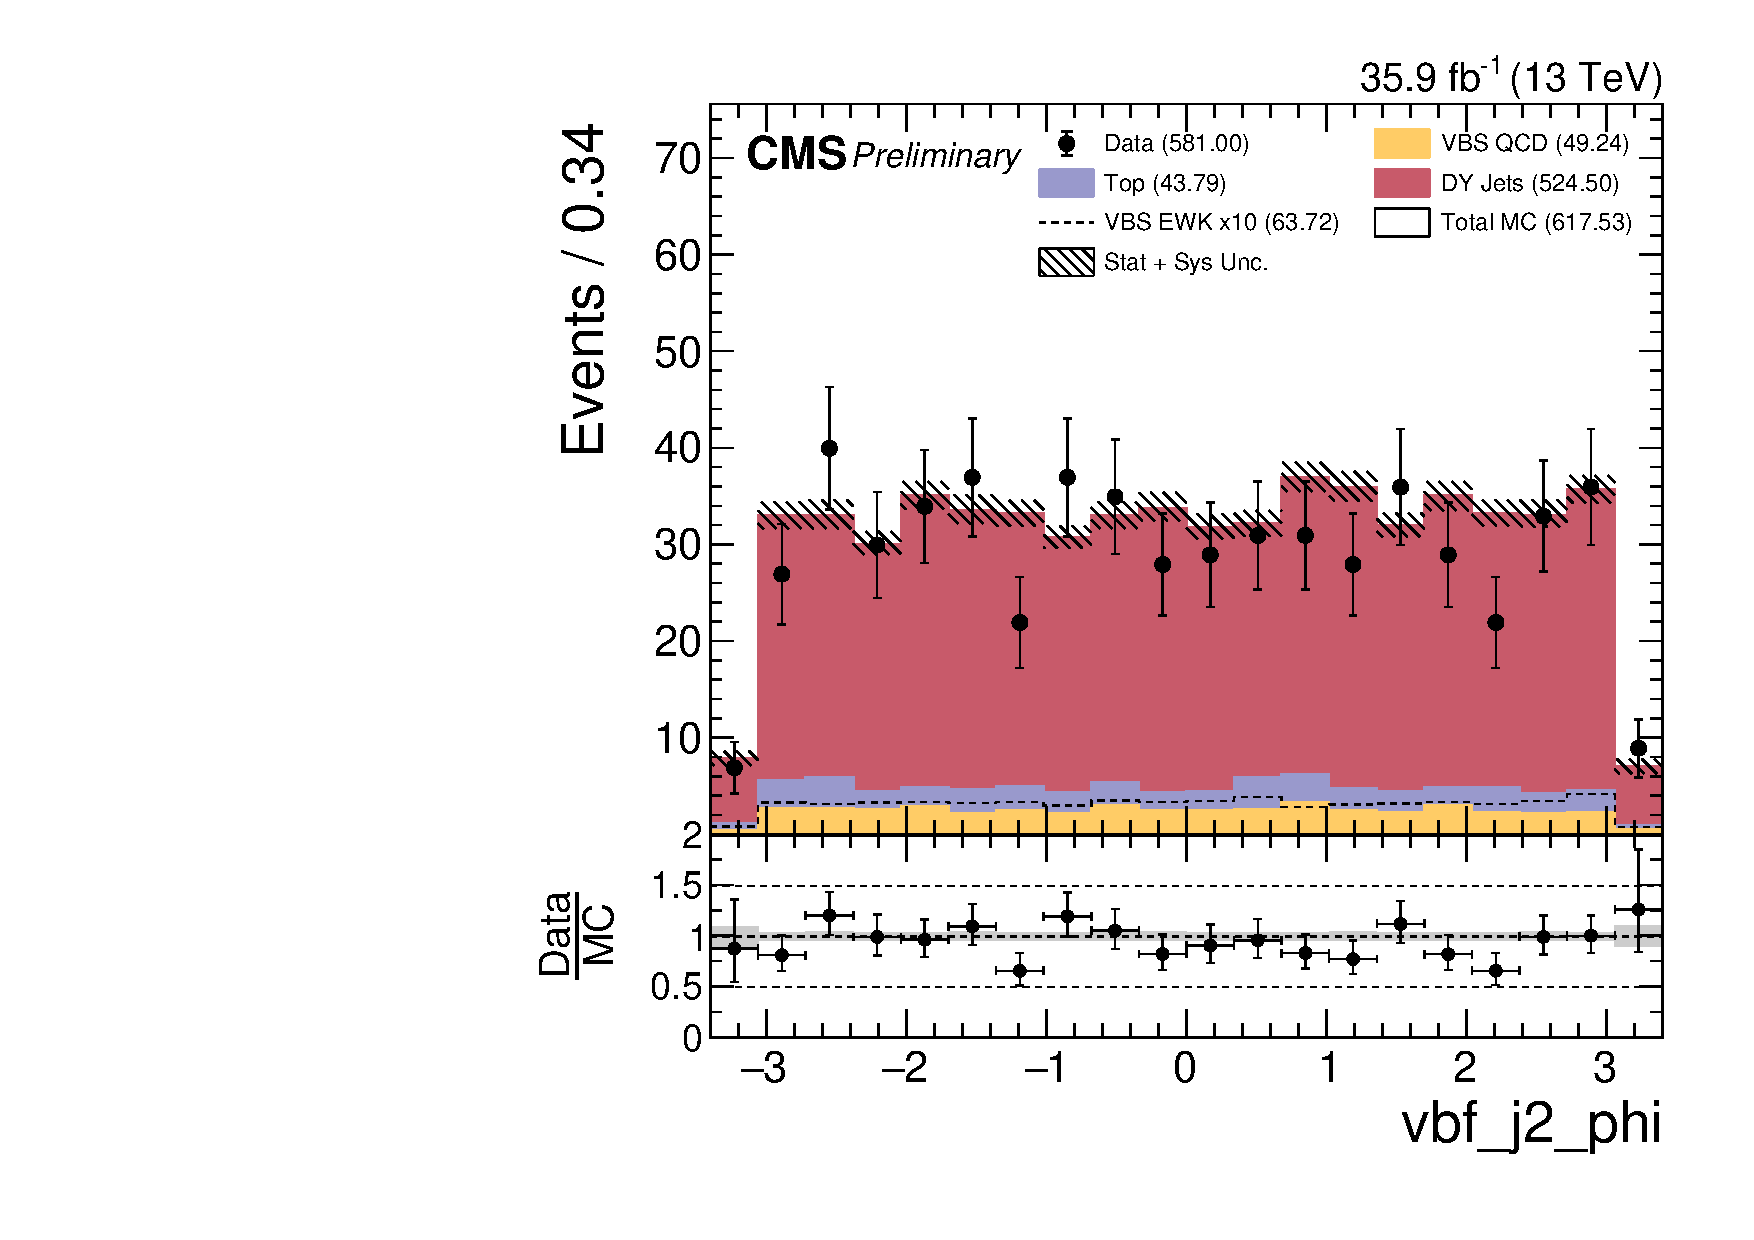
\includegraphics[width=0.335\textwidth]{analysis_plots/2016_zv/cr_vjets_l/vbf_j2_phi.pdf} \hspace{-10pt}
  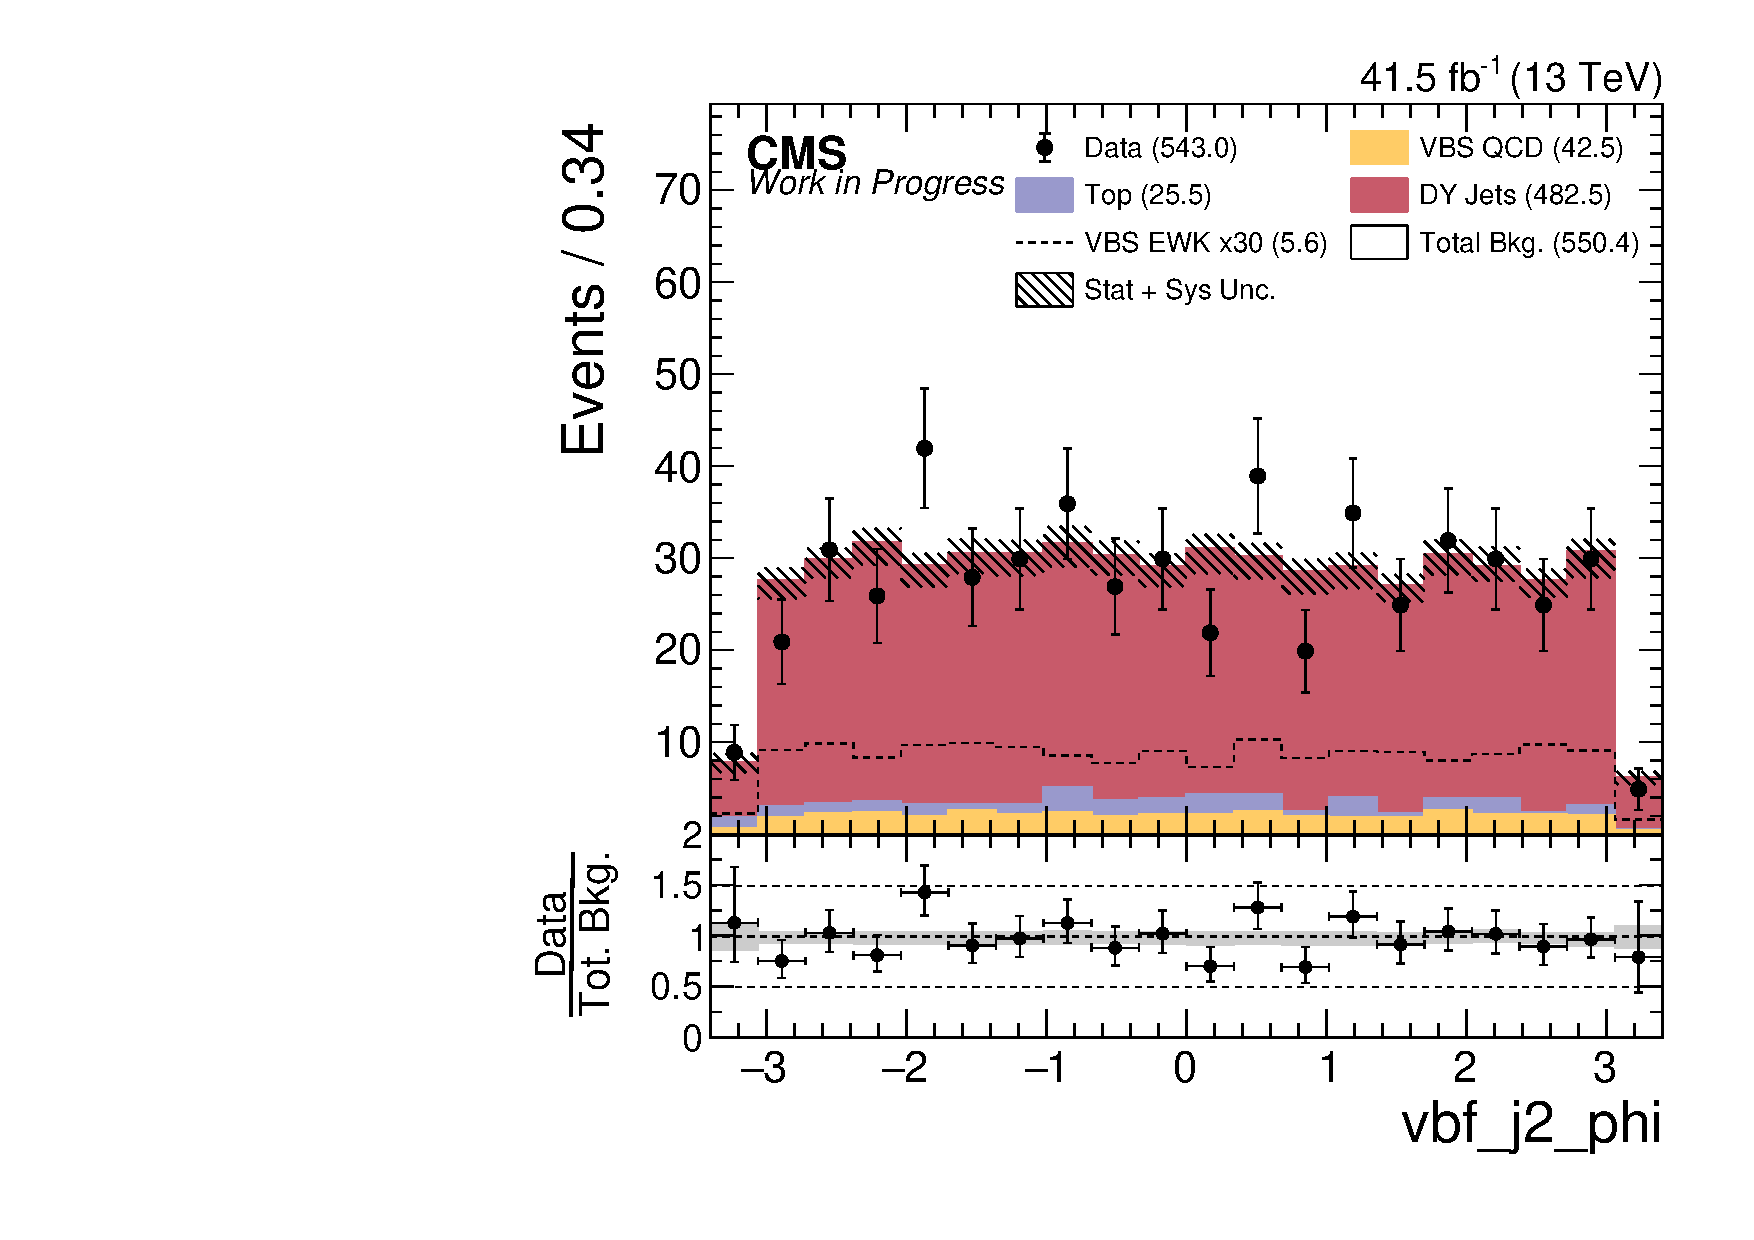
\includegraphics[width=0.335\textwidth]{analysis_plots/2017_zv/cr_vjets_l/vbf_j2_phi.pdf} \hspace{-10pt}
  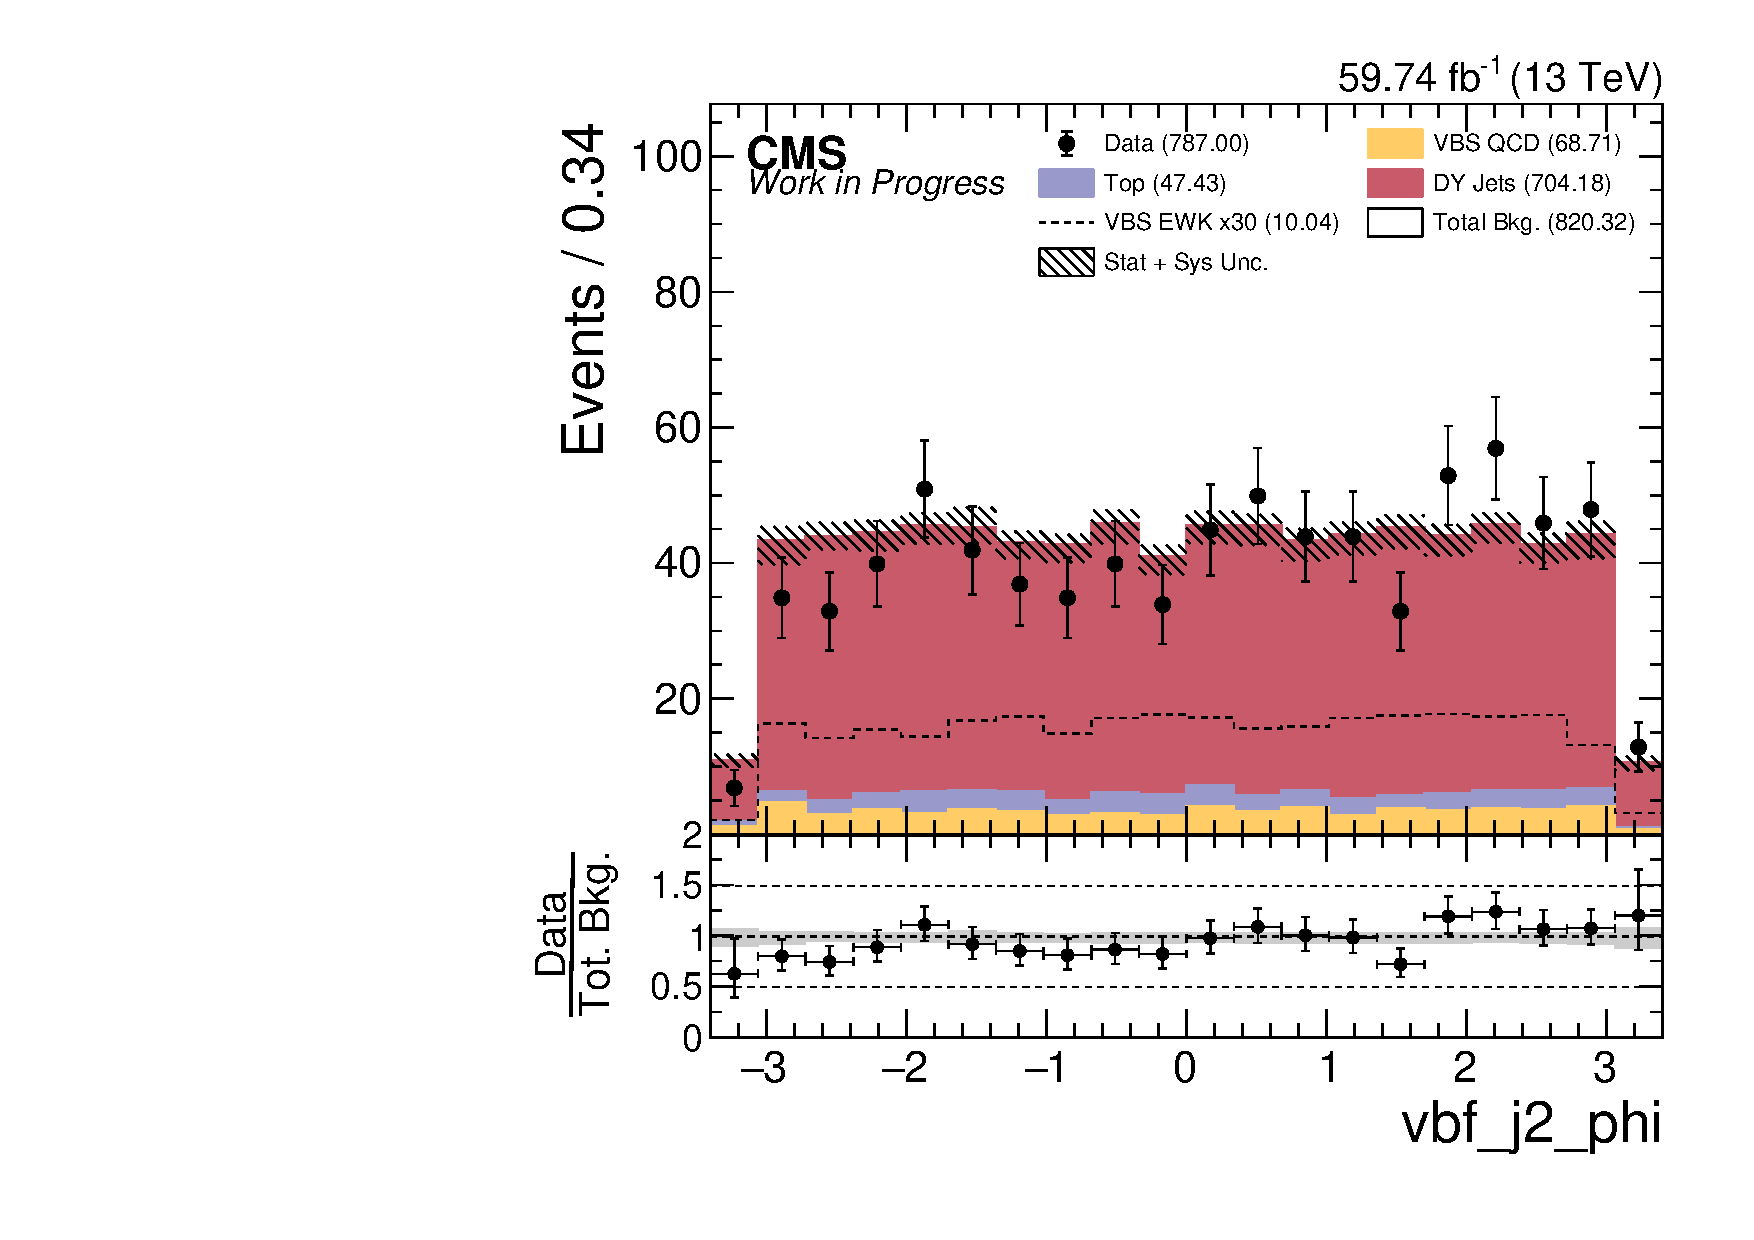
\includegraphics[width=0.335\textwidth]{analysis_plots/2018_zv/cr_vjets_l/vbf_j2_phi.pdf} \hspace{-10pt} \\
  \caption[DY+Jets Control Region: Trailing VBS tagged jet kinematics in Boosted ZV Channel]%
  {DY+Jets Control Region: Trailing VBS tagged jet kinematics in Boosted ZV Channel.
    Error bars include statistical uncertainty on total background,
    JES and QCD scale systematic on DY+Jets and VBS\_QCD MC\@. From Left to Right: 2016,
    2017, and 2018. From Top to Bottom: \( p_T \), \( \eta \), and \( \phi \).}%
  \label{fig:zv-cr-vjets-l-vbs2-pt-eta-m}
\end{figure}

\clearpage
\subsection{
  Resolved ZV DY+Jets Control Region
}\label{ch_vbs:resolved-plots}

\begin{figure}[!ht]
  \centering
  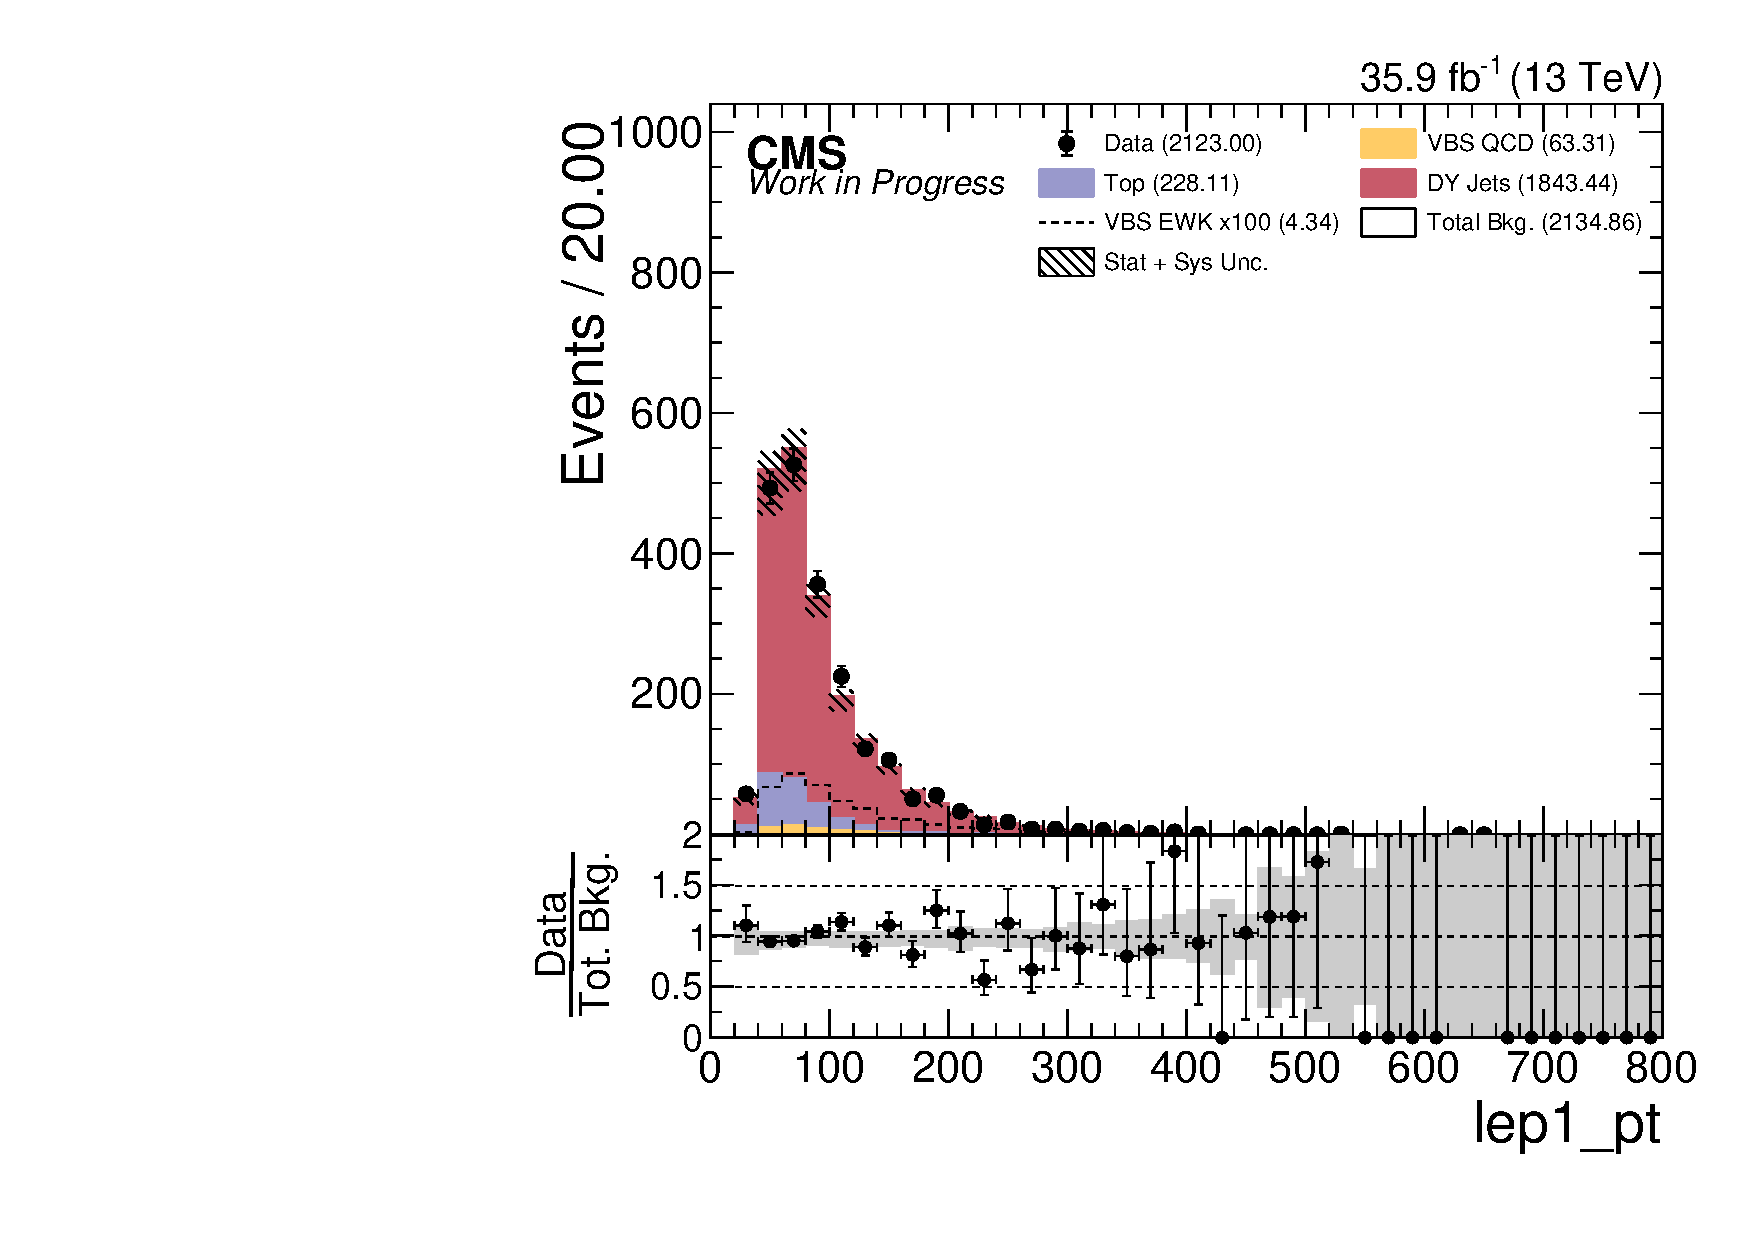
\includegraphics[width=0.335\textwidth]{analysis_plots/2016_zjj/cr_vjets_e/lep1_pt.pdf} \hspace{-10pt}
  \includegraphics[width=0.335\textwidth]{analysis_plots/2017_zjj/cr_vjets_e/lep1_pt.pdf} \hspace{-10pt}
  \includegraphics[width=0.335\textwidth]{analysis_plots/2018_zjj/cr_vjets_e/lep1_pt.pdf} \hspace{-10pt} \\
  \includegraphics[width=0.335\textwidth]{analysis_plots/2016_zjj/cr_vjets_e/lep1_eta.pdf} \hspace{-10pt}
  \includegraphics[width=0.335\textwidth]{analysis_plots/2017_zjj/cr_vjets_e/lep1_eta.pdf} \hspace{-10pt}
  \includegraphics[width=0.335\textwidth]{analysis_plots/2018_zjj/cr_vjets_e/lep1_eta.pdf} \hspace{-10pt} \\
  \includegraphics[width=0.335\textwidth]{analysis_plots/2016_zjj/cr_vjets_e/lep1_phi.pdf} \hspace{-10pt}
  \includegraphics[width=0.335\textwidth]{analysis_plots/2017_zjj/cr_vjets_e/lep1_phi.pdf} \hspace{-10pt}
  \includegraphics[width=0.335\textwidth]{analysis_plots/2018_zjj/cr_vjets_e/lep1_phi.pdf} \hspace{-10pt} \\
  \caption[DY+Jets Control Region: Leading electron kinematics in Resolved ZV Channel]%
  {DY+Jets Control Region: Leading electron kinematics in Resolved ZV Channel.
    Error bars include statistical uncertainty on total background,
    JES and QCD scale systematic on DY+Jets and VBS\_QCD MC\@. From Left to Right: 2016,
    2017, and 2018. From Top to Bottom: \( p_T \), \( \eta \), and \( \phi \).}%
  \label{fig:zjj-cr-vjets-e-lep1-pt-eta-phi}
\end{figure}

\begin{figure}[!ht]
  \centering
  \includegraphics[width=0.335\textwidth]{analysis_plots/2016_zjj/cr_vjets_m/lep1_pt.pdf} \hspace{-10pt}
  \includegraphics[width=0.335\textwidth]{analysis_plots/2017_zjj/cr_vjets_m/lep1_pt.pdf} \hspace{-10pt}
  \includegraphics[width=0.335\textwidth]{analysis_plots/2018_zjj/cr_vjets_m/lep1_pt.pdf} \hspace{-10pt} \\
  \includegraphics[width=0.335\textwidth]{analysis_plots/2016_zjj/cr_vjets_m/lep1_eta.pdf} \hspace{-10pt}
  \includegraphics[width=0.335\textwidth]{analysis_plots/2017_zjj/cr_vjets_m/lep1_eta.pdf} \hspace{-10pt}
  \includegraphics[width=0.335\textwidth]{analysis_plots/2018_zjj/cr_vjets_m/lep1_eta.pdf} \hspace{-10pt} \\
  \includegraphics[width=0.335\textwidth]{analysis_plots/2016_zjj/cr_vjets_m/lep1_phi.pdf} \hspace{-10pt}
  \includegraphics[width=0.335\textwidth]{analysis_plots/2017_zjj/cr_vjets_m/lep1_phi.pdf} \hspace{-10pt}
  \includegraphics[width=0.335\textwidth]{analysis_plots/2018_zjj/cr_vjets_m/lep1_phi.pdf} \hspace{-10pt} \\
  \caption[DY+Jets Control Region: Leading muon kinematics in Resolved ZV Channel]%
  {DY+Jets Control Region: Leading muon kinematics in Resolved ZV Channel.
    Error bars include statistical uncertainty on total background,
    JES and QCD scale systematic on DY+Jets and VBS\_QCD MC\@. From Left to Right: 2016,
    2017, and 2018. From Top to Bottom: \( p_T \), \( \eta \), and \( \phi \).}%
  \label{fig:zjj-cr-vjets-m-lep1-pt-eta-phi}
\end{figure}

\begin{figure}[!ht]
  \centering
  \includegraphics[width=0.335\textwidth]{analysis_plots/2016_zjj/cr_vjets_l/dijet_j1_pt.pdf} \hspace{-10pt}
  \includegraphics[width=0.335\textwidth]{analysis_plots/2017_zjj/cr_vjets_l/dijet_j1_pt.pdf} \hspace{-10pt}
  \includegraphics[width=0.335\textwidth]{analysis_plots/2018_zjj/cr_vjets_l/dijet_j1_pt.pdf} \hspace{-10pt} \\
  \includegraphics[width=0.335\textwidth]{analysis_plots/2016_zjj/cr_vjets_l/dijet_j2_pt.pdf} \hspace{-10pt}
  \includegraphics[width=0.335\textwidth]{analysis_plots/2017_zjj/cr_vjets_l/dijet_j2_pt.pdf} \hspace{-10pt}
  \includegraphics[width=0.335\textwidth]{analysis_plots/2018_zjj/cr_vjets_l/dijet_j2_pt.pdf} \hspace{-10pt} \\
  \includegraphics[width=0.335\textwidth]{analysis_plots/2016_zjj/cr_vjets_l/dijet_m.pdf} \hspace{-10pt}
  \includegraphics[width=0.335\textwidth]{analysis_plots/2017_zjj/cr_vjets_l/dijet_m.pdf} \hspace{-10pt}
  \includegraphics[width=0.335\textwidth]{analysis_plots/2018_zjj/cr_vjets_l/dijet_m.pdf} \hspace{-10pt} \\
  \caption[DY+Jets Control Region: Hadronic boson leading and trailing jet \(p_T\) in Resolved ZV Channel]%
  {DY+Jets Control Region: Hadronic boson leading and trailing jet \(p_T\) in Resolved ZV Channel.
    Error bars include statistical uncertainty on total background,
    JES and QCD scale systematic on DY+Jets and VBS\_QCD MC\@. From Left to Right: 2016,
    2017, and 2018. From Top to Bottom: \( p_T \) of leading jet, \(p_T\) of trailing jet, and invariant mass \( m_{jj} \).}%
  \label{fig:zjj-cr-vjets-l-dijet1-pt-eta-m}
\end{figure}

\begin{figure}[!ht]
  \centering
  \includegraphics[width=0.335\textwidth]{analysis_plots/2016_zjj/cr_vjets_l/vbf_j1_pt.pdf} \hspace{-10pt}
  \includegraphics[width=0.335\textwidth]{analysis_plots/2017_zjj/cr_vjets_l/vbf_j1_pt.pdf} \hspace{-10pt}
  \includegraphics[width=0.335\textwidth]{analysis_plots/2018_zjj/cr_vjets_l/vbf_j1_pt.pdf} \hspace{-10pt} \\
  \includegraphics[width=0.335\textwidth]{analysis_plots/2016_zjj/cr_vjets_l/vbf_j1_eta.pdf} \hspace{-10pt}
  \includegraphics[width=0.335\textwidth]{analysis_plots/2017_zjj/cr_vjets_l/vbf_j1_eta.pdf} \hspace{-10pt}
  \includegraphics[width=0.335\textwidth]{analysis_plots/2018_zjj/cr_vjets_l/vbf_j1_eta.pdf} \hspace{-10pt} \\
  \includegraphics[width=0.335\textwidth]{analysis_plots/2016_zjj/cr_vjets_l/vbf_j1_phi.pdf} \hspace{-10pt}
  \includegraphics[width=0.335\textwidth]{analysis_plots/2017_zjj/cr_vjets_l/vbf_j1_phi.pdf} \hspace{-10pt}
  \includegraphics[width=0.335\textwidth]{analysis_plots/2018_zjj/cr_vjets_l/vbf_j1_phi.pdf} \hspace{-10pt} \\
  \caption[DY+Jets Control Region: Leading VBS tagged jet kinematics in Resolved ZV Channel]%
  {DY+Jets Control Region: Leading VBS tagged jet kinematics in Resolved ZV Channel.
    Error bars include statistical uncertainty on total background,
    JES and QCD scale systematic on DY+Jets and VBS\_QCD MC\@. From Left to Right: 2016,
    2017, and 2018. From Top to Bottom: \( p_T \), \( \eta \), and \( \phi \).}%
  \label{fig:zjj-cr-vjets-l-vbs1-pt-eta-m}
\end{figure}

\begin{figure}[!ht]
  \centering
  \includegraphics[width=0.335\textwidth]{analysis_plots/2016_zjj/cr_vjets_l/vbf_j2_pt.pdf} \hspace{-10pt}
  \includegraphics[width=0.335\textwidth]{analysis_plots/2017_zjj/cr_vjets_l/vbf_j2_pt.pdf} \hspace{-10pt}
  \includegraphics[width=0.335\textwidth]{analysis_plots/2018_zjj/cr_vjets_l/vbf_j2_pt.pdf} \hspace{-10pt} \\
  \includegraphics[width=0.335\textwidth]{analysis_plots/2016_zjj/cr_vjets_l/vbf_j2_eta.pdf} \hspace{-10pt}
  \includegraphics[width=0.335\textwidth]{analysis_plots/2017_zjj/cr_vjets_l/vbf_j2_eta.pdf} \hspace{-10pt}
  \includegraphics[width=0.335\textwidth]{analysis_plots/2018_zjj/cr_vjets_l/vbf_j2_eta.pdf} \hspace{-10pt} \\
  \includegraphics[width=0.335\textwidth]{analysis_plots/2016_zjj/cr_vjets_l/vbf_j2_phi.pdf} \hspace{-10pt}
  \includegraphics[width=0.335\textwidth]{analysis_plots/2017_zjj/cr_vjets_l/vbf_j2_phi.pdf} \hspace{-10pt}
  \includegraphics[width=0.335\textwidth]{analysis_plots/2018_zjj/cr_vjets_l/vbf_j2_phi.pdf} \hspace{-10pt} \\
  \caption[DY+Jets Control Region: Trailing VBS tagged jet kinematics in Resolved ZV Channel]%
  {DY+Jets Control Region: Trailing VBS tagged jet kinematics in Resolved ZV Channel.
    Error bars include statistical uncertainty on total background,
    JES and QCD scale systematic on DY+Jets and VBS\_QCD MC\@. From Left to Right: 2016,
    2017, and 2018. From Top to Bottom: \( p_T \), \( \eta \), and \( \phi \).}%
  \label{fig:zjj-cr-vjets-l-vbs2-pt-eta-m}
\end{figure}

\clearpage
\section{
  Machine Learning Modeling
 }

Instead of traditional cut-based analysis, we decided to use \glsfirst{MVA} a.k.a. \glsfirst{ML}
technique to build a signal vs background classifier. The main reasoning behind using
a \gls{MVA} technique is so that we can build a model which can learn our
analysis topology from looser selection regions and still let us keep higher statistics
for final measurement.

\subsection{
  Algorithm: Gradient Boosted Decision Tree
}

\textit{Boosting} is a method of combining many weak learners sequentially into
single classifier. In \gls{BDT} boosting is applied to \textit{decision tree}.
A decision tree is a binary tree,
example shown in Figure~\ref{fig:bdt-dt}, at each node
a decision is made using the input variables which
provides the best separation\footnote{defined as,
  \( \frac{1}{2}
  \int \frac{{(\hat{y}_{S}(y) - \hat{y}_{B}(y))}^2}{\hat{y}_{S}(y) + \hat{y}_{B}(y)} dy \),
  where \(\hat{y}_{S}\) and \(\hat{y}_B\) are probability density functions
  of signal and background.}
at that node, this process is repeated
until events at a node reaches below certain threshold, and then depending
on the majority
of the events in the final node, the node is classified
as signal or background.

There are several boosting algorithms, the one discussed and
used in this analysis is the gradient boost.
Gradient boost is an additive model of adding decision trees
in series and with each tree in the sequence, training on
the adjusted dataset to minimize the \textit{loss function} with
respect to the previous model. The role of the loss function is to estimate
the difference between actual and predicted values. This improves
the model sequentially and is faster since only a subset of
training dataset is used in subsequent decision trees.
\gls{TMVA}, part of \ROOT{} package is used in this analysis
for implementing the gradient \gls{BDT}
of binomial log-likelihood loss function for classification~\cite{tmva-manual}.

\begin{figure}
  \centering
  \includegraphics[width=0.6\textwidth]{figures/bdt_pics.pdf}
  \caption[Decision Tree]{Decision Tree.}%
  \label{fig:bdt-dt}
\end{figure}

\subsection{
  Training and Results
}

Two models were trained for boosted and resolved topology.
The training was done using combined MC from all years 2016, 2017, 2018
to benefit from larger statistics (see Table~\ref{tab:training-stats}).
Signal MC ``VBS\_EWK'' was trained against background ``DY + Jets LO'' since
that is dominant background in our analysis.
The learning process of \gls{MVA} algorithm is tuned by hyper-parameters values.
Each models \gls{BDT} hyper-parameters were tuned to prevent under and over-fitting.
This is done by comparing the signal efficiency for
training and testing datasets at three different background rates (1\%, 10\% and 30\%).
If the difference is not more than 5\%, then the hyper-parameters are
acceptable.

\gls{ROC} is a way to visualize performance of signal vs.\ background efficiency.
\gls{AUC} of \gls{ROC} is a measure of the classifier to distinguish signal from background.
\gls{AUC} of above 50\% means that classifier will be able to distinguish from signal
from background events.

Input variables used in each training model were pruned i.e.
input variables which do not have significant impact on the
performance of the model in terms of \gls{AUC} of \gls{ROC}
were dropped from the final training models.
Distribution of final input variables
used in training are shown in Figures~\ref{fig:vbs-training-input-zv} --~\ref{fig:vbs-training-input-zjj-1-sr}.

\begin{table}[!ht]
  \centering
  \caption{Combined dataset Training and Testing Statistics in Signal Region}
  \begin{tabular}{lllll}%
    \toprule
             &            & \multicolumn{3}{c}{Number of Events}                    \\
    \cmidrule(lr){3-5}
    Channel  & Dataset    & Training                             & Testing & Total  \\
    \midrule
    Boosted  & Signal     & 7404                                 & 7405    & 14809  \\
    Boosted  & Background & 46991                                & 46991   & 93982  \\
    \midrule
    Resolved & Signal     & 23425                                & 23425   & 46850  \\
    Resolved & Background & 209368                               & 209368  & 418736 \\
    \bottomrule
  \end{tabular}\label{tab:training-stats}
\end{table}


Final input variables used in Boosted and Resolved \textit{ZV} training model are:
\begin{itemize}
  \item \( M_{JJ}^{VBS} \): invariant mass of \gls{VBS} tagged jets.
  \item Zeppenfeld \( z^{*} \): Zeppenfeld variable for \textit{Z} boson~\cite{Rainwater1996}, \( z^{*} = \frac{\eta_{Z} - (\eta_{j1}^{VBS} + \eta_{j2}^{VBS})/2}{|\Delta \eta_{jj}^{VBS}|} \)
  \item QGL \( j_{1}^{VBS} \), \( j_{2}^{VBS} \): \gls{QGL} of VBS tagged jets. Likelihood whether the jet originated from a quark or gluon.
  \item \( M_{VV} \) invariant mass of \textit{Z} and \textit{V} boson.
  \item HT\textsuperscript{*} (Resolved category only): scalar sum of \(p_T\) of jet candidates
        of \textit{V} boson and \gls{VBS} tagged jets.
  \item \( \eta_{lep2} \) (Resolved category only): \( \eta \) of trailing lepton.
\end{itemize}


\begin{figure}[!ht]
  \centering
  \includegraphics[width=0.235\textwidth]{analysis_plots/tmva_plots/zv_BDTG14_dibos_m.pdf} \hspace{-12pt}
  \includegraphics[width=0.235\textwidth]{analysis_plots/2016_zv/cr_vjets_l/vv_m.pdf} \hspace{-12pt}
  \includegraphics[width=0.235\textwidth]{analysis_plots/2017_zv/cr_vjets_l/vv_m.pdf} \hspace{-12pt}
  \includegraphics[width=0.235\textwidth]{analysis_plots/2018_zv/cr_vjets_l/vv_m.pdf} \hspace{-12pt} \\ \vspace{-1pt}
  \includegraphics[width=0.235\textwidth]{analysis_plots/tmva_plots/zv_BDTG14_vbf_m.pdf} \hspace{-12pt}
  \includegraphics[width=0.235\textwidth]{analysis_plots/2016_zv/cr_vjets_l/vbf_jj_m.pdf} \hspace{-12pt}
  \includegraphics[width=0.235\textwidth]{analysis_plots/2017_zv/cr_vjets_l/vbf_jj_m.pdf} \hspace{-12pt}
  \includegraphics[width=0.235\textwidth]{analysis_plots/2018_zv/cr_vjets_l/vbf_jj_m.pdf} \hspace{-12pt} \\ \vspace{-1pt}
  \includegraphics[width=0.235\textwidth]{analysis_plots/tmva_plots/zv_BDTG14_vbf1_AK4_qgid.pdf} \hspace{-12pt}
  \includegraphics[width=0.235\textwidth]{analysis_plots/2016_zv/cr_vjets_l/vbf_j1_qgid.pdf} \hspace{-12pt}
  \includegraphics[width=0.235\textwidth]{analysis_plots/2017_zv/cr_vjets_l/vbf_j1_qgid.pdf} \hspace{-12pt}
  \includegraphics[width=0.235\textwidth]{analysis_plots/2018_zv/cr_vjets_l/vbf_j1_qgid.pdf} \hspace{-12pt} \\ \vspace{-1pt}
  \includegraphics[width=0.235\textwidth]{analysis_plots/tmva_plots/zv_BDTG14_vbf2_AK4_qgid.pdf} \hspace{-12pt}
  \includegraphics[width=0.235\textwidth]{analysis_plots/2016_zv/cr_vjets_l/vbf_j2_qgid.pdf} \hspace{-12pt}
  \includegraphics[width=0.235\textwidth]{analysis_plots/2017_zv/cr_vjets_l/vbf_j2_qgid.pdf} \hspace{-12pt}
  \includegraphics[width=0.235\textwidth]{analysis_plots/2018_zv/cr_vjets_l/vbf_j2_qgid.pdf} \hspace{-12pt} \\ \vspace{-1pt}
  \includegraphics[width=0.235\textwidth]{analysis_plots/tmva_plots/zv_BDTG14_zeppLep_deta.pdf} \hspace{-12pt}
  \includegraphics[width=0.235\textwidth]{analysis_plots/2016_zv/cr_vjets_l/zeppenfeld_lep_deta.pdf} \hspace{-12pt}
  \includegraphics[width=0.235\textwidth]{analysis_plots/2017_zv/cr_vjets_l/zeppenfeld_lep_deta.pdf} \hspace{-12pt}
  \includegraphics[width=0.235\textwidth]{analysis_plots/2018_zv/cr_vjets_l/zeppenfeld_lep_deta.pdf} \hspace{-12pt} \\ \vspace{-1pt}
  \caption[Inputs Variables for training Boosted ZV BDT Classifier]%
  {Inputs Variables for training Boosted ZV BDT Classifier.
    Left to Right: Shape comparison of signal and background (combined dataset), control region
    kinematic distribution in 2016, 2017 and 2018 dataset.
    Top to Bottom: Diboson invariant mass, VBS tagged jets invariant mass, QGL of leading
    VBS tagged jet, QGL of trailing VBS tagged jet, Zeppenfeld variable of leptonic boson.}%
  \label{fig:vbs-training-input-zv}
\end{figure}

\begin{figure}[!ht]
  \centering
  \includegraphics[width=0.25\textwidth]{analysis_plots/2016_zv/sr_l/vv_m.pdf} \hspace{-12pt}
  \includegraphics[width=0.25\textwidth]{analysis_plots/2017_zv/sr_l/vv_m.pdf} \hspace{-12pt}
  \includegraphics[width=0.25\textwidth]{analysis_plots/2018_zv/sr_l/vv_m.pdf} \hspace{-12pt} \\ \vspace{-5pt}
  \includegraphics[width=0.25\textwidth]{analysis_plots/2016_zv/sr_l/vbf_jj_m.pdf} \hspace{-12pt}
  \includegraphics[width=0.25\textwidth]{analysis_plots/2017_zv/sr_l/vbf_jj_m.pdf} \hspace{-12pt}
  \includegraphics[width=0.25\textwidth]{analysis_plots/2018_zv/sr_l/vbf_jj_m.pdf} \hspace{-12pt} \\ \vspace{-5pt}
  \includegraphics[width=0.25\textwidth]{analysis_plots/2016_zv/sr_l/vbf_j1_qgid.pdf} \hspace{-12pt}
  \includegraphics[width=0.25\textwidth]{analysis_plots/2017_zv/sr_l/vbf_j1_qgid.pdf} \hspace{-12pt}
  \includegraphics[width=0.25\textwidth]{analysis_plots/2018_zv/sr_l/vbf_j1_qgid.pdf} \hspace{-12pt} \\ \vspace{-5pt}
  \includegraphics[width=0.25\textwidth]{analysis_plots/2016_zv/sr_l/vbf_j2_qgid.pdf} \hspace{-12pt}
  \includegraphics[width=0.25\textwidth]{analysis_plots/2017_zv/sr_l/vbf_j2_qgid.pdf} \hspace{-12pt}
  \includegraphics[width=0.25\textwidth]{analysis_plots/2018_zv/sr_l/vbf_j2_qgid.pdf} \hspace{-12pt} \\ \vspace{-5pt}
  \includegraphics[width=0.25\textwidth]{analysis_plots/2016_zv/sr_l/zeppenfeld_lep_deta.pdf} \hspace{-12pt}
  \includegraphics[width=0.25\textwidth]{analysis_plots/2017_zv/sr_l/zeppenfeld_lep_deta.pdf} \hspace{-12pt}
  \includegraphics[width=0.25\textwidth]{analysis_plots/2018_zv/sr_l/zeppenfeld_lep_deta.pdf} \hspace{-12pt} \\ \vspace{-5pt}
  \caption[Inputs Variables for training Boosted ZV BDT Classifier in signal region.]%
  {Inputs Variables for training Boosted ZV BDT Classifier in signal region.
    Left to Right: 2016, 2017 and 2018 dataset.
    Top to Bottom: Diboson invariant mass, VBS tagged jets invariant mass, QGL of leading
    VBS tagged jet, QGL of trailing VBS tagged jet, Zeppenfeld variable of leptonic boson.}%
  \label{fig:vbs-training-input-zv-sr}
\end{figure}


\begin{figure}[!ht]
  \centering
  \includegraphics[width=0.25\textwidth]{analysis_plots/tmva_plots/zjj_BDTG14_dibos_m.pdf} \hspace{-10pt}
  \includegraphics[width=0.25\textwidth]{analysis_plots/2016_zjj/cr_vjets_l/vv_m.pdf} \hspace{-10pt}
  \includegraphics[width=0.25\textwidth]{analysis_plots/2017_zjj/cr_vjets_l/vv_m.pdf} \hspace{-10pt}
  \includegraphics[width=0.25\textwidth]{analysis_plots/2018_zjj/cr_vjets_l/vv_m.pdf} \hspace{-10pt}  \\
  \includegraphics[width=0.25\textwidth]{analysis_plots/tmva_plots/zjj_BDTG14_vbf_m.pdf} \hspace{-10pt}
  \includegraphics[width=0.25\textwidth]{analysis_plots/2016_zjj/cr_vjets_l/vbf_jj_m.pdf} \hspace{-10pt}
  \includegraphics[width=0.25\textwidth]{analysis_plots/2017_zjj/cr_vjets_l/vbf_jj_m.pdf} \hspace{-10pt}
  \includegraphics[width=0.25\textwidth]{analysis_plots/2018_zjj/cr_vjets_l/vbf_jj_m.pdf} \hspace{-10pt} \\
  \includegraphics[width=0.25\textwidth]{analysis_plots/tmva_plots/zjj_BDTG14_ht_resolved.pdf} \hspace{-10pt}
  \includegraphics[width=0.25\textwidth]{analysis_plots/2018_zjj/cr_vjets_l/ht_resolved.pdf} \hspace{-10pt}
  \includegraphics[width=0.25\textwidth]{analysis_plots/2018_zjj/cr_vjets_l/ht_resolved.pdf} \hspace{-10pt}
  \includegraphics[width=0.25\textwidth]{analysis_plots/2018_zjj/cr_vjets_l/ht_resolved.pdf} \hspace{-10pt} \\
  \includegraphics[width=0.25\textwidth]{analysis_plots/tmva_plots/zjj_BDTG14_lep2_eta.pdf} \hspace{-10pt}
  \includegraphics[width=0.25\textwidth]{analysis_plots/2016_zjj/cr_vjets_l/lep2_eta.pdf} \hspace{-10pt}
  \includegraphics[width=0.25\textwidth]{analysis_plots/2017_zjj/cr_vjets_l/lep2_eta.pdf} \hspace{-10pt}
  \includegraphics[width=0.25\textwidth]{analysis_plots/2018_zjj/cr_vjets_l/lep2_eta.pdf} \hspace{-10pt}
  \caption[Inputs Variables for training Resolved ZV BDT Classifier]%
  {Inputs Variables for training Resolved ZV BDT Classifier.
    Left to Right: Shape comparison of signal and background (combined dataset), control region
    kinematic distribution in 2016, 2017 and 2018 dataset.
    Top to Bottom: Diboson invariant mass, VBS tagged jets invariant mass,
    HT\textsuperscript{*} (\( p_{T} \) sum of jets), trailing lepton \( \eta \).}%
  \label{fig:vbs-training-input-zjj}
\end{figure}

\begin{figure}[!ht]
  \centering
  \includegraphics[width=0.30\textwidth]{analysis_plots/2016_zjj/cr_vjets_l/vv_m.pdf} \hspace{-10pt}
  \includegraphics[width=0.30\textwidth]{analysis_plots/2017_zjj/cr_vjets_l/vv_m.pdf} \hspace{-10pt}
  \includegraphics[width=0.30\textwidth]{analysis_plots/2018_zjj/cr_vjets_l/vv_m.pdf} \hspace{-10pt}  \\
  \includegraphics[width=0.30\textwidth]{analysis_plots/2016_zjj/cr_vjets_l/vbf_jj_m.pdf} \hspace{-10pt}
  \includegraphics[width=0.30\textwidth]{analysis_plots/2017_zjj/cr_vjets_l/vbf_jj_m.pdf} \hspace{-10pt}
  \includegraphics[width=0.30\textwidth]{analysis_plots/2018_zjj/cr_vjets_l/vbf_jj_m.pdf} \hspace{-10pt} \\
  \includegraphics[width=0.30\textwidth]{analysis_plots/2018_zjj/cr_vjets_l/ht_resolved.pdf} \hspace{-10pt}
  \includegraphics[width=0.30\textwidth]{analysis_plots/2018_zjj/cr_vjets_l/ht_resolved.pdf} \hspace{-10pt}
  \includegraphics[width=0.30\textwidth]{analysis_plots/2018_zjj/cr_vjets_l/ht_resolved.pdf} \hspace{-10pt} \\
  \includegraphics[width=0.30\textwidth]{analysis_plots/2016_zjj/cr_vjets_l/lep2_eta.pdf} \hspace{-10pt}
  \includegraphics[width=0.30\textwidth]{analysis_plots/2017_zjj/cr_vjets_l/lep2_eta.pdf} \hspace{-10pt}
  \includegraphics[width=0.30\textwidth]{analysis_plots/2018_zjj/cr_vjets_l/lep2_eta.pdf} \hspace{-10pt}
  \caption[Inputs Variables for training Resolved ZV BDT Classifier in signal region.]%
  {Inputs Variables for training Resolved ZV BDT Classifier in signal region.
    Left to Right: 2016, 2017 and 2018 dataset.
    Top to Bottom: Diboson invariant mass, VBS tagged jets invariant mass,
    HT\textsuperscript{*} (\( p_{T} \) sum of jets), trailing lepton \( \eta \).}%
  \label{fig:vbs-training-input-zjj-sr}
\end{figure}

\begin{figure}[!ht]
  \centering
  \includegraphics[width=0.25\textwidth]{analysis_plots/tmva_plots/zjj_BDTG14_vbf1_AK4_qgid.pdf} \hspace{-10pt}
  \includegraphics[width=0.25\textwidth]{analysis_plots/2016_zjj/cr_vjets_l/vbf_j1_qgid.pdf} \hspace{-10pt}
  \includegraphics[width=0.25\textwidth]{analysis_plots/2017_zjj/cr_vjets_l/vbf_j1_qgid.pdf} \hspace{-10pt}
  \includegraphics[width=0.25\textwidth]{analysis_plots/2018_zjj/cr_vjets_l/vbf_j1_qgid.pdf} \hspace{-10pt}  \\
  \includegraphics[width=0.25\textwidth]{analysis_plots/tmva_plots/zjj_BDTG14_vbf2_AK4_qgid.pdf} \hspace{-10pt}
  \includegraphics[width=0.25\textwidth]{analysis_plots/2016_zjj/cr_vjets_l/vbf_j2_qgid.pdf} \hspace{-10pt}
  \includegraphics[width=0.25\textwidth]{analysis_plots/2017_zjj/cr_vjets_l/vbf_j2_qgid.pdf} \hspace{-10pt}
  \includegraphics[width=0.25\textwidth]{analysis_plots/2018_zjj/cr_vjets_l/vbf_j2_qgid.pdf} \hspace{-10pt}  \\
  \includegraphics[width=0.25\textwidth]{analysis_plots/tmva_plots/zjj_BDTG14_zeppLep_deta.pdf} \hspace{-10pt}
  \includegraphics[width=0.25\textwidth]{analysis_plots/2016_zjj/cr_vjets_l/zeppenfeld_lep_deta.pdf} \hspace{-10pt}
  \includegraphics[width=0.25\textwidth]{analysis_plots/2017_zjj/cr_vjets_l/zeppenfeld_lep_deta.pdf} \hspace{-10pt}
  \includegraphics[width=0.25\textwidth]{analysis_plots/2018_zjj/cr_vjets_l/zeppenfeld_lep_deta.pdf} \hspace{-10pt}
  \caption[Inputs Variables for training Resolved ZV BDT Classifier]%
  {Inputs Variables for training Resolved ZV BDT Classifier.
    Left to Right: Shape comparison of signal and background (combined dataset), control region
    kinematic distribution in 2016, 2017 and 2018 dataset.
    Top to Bottom: QGL of leading VBS tagged jet,
    QGL of trailing VBS tagged jet, Zeppenfeld variable of leptonic boson.}%
  \label{fig:vbs-training-input-zjj-1}
\end{figure}

\begin{figure}[!ht]
  \centering
  \includegraphics[width=0.33\textwidth]{analysis_plots/2016_zjj/sr_l/vbf_j1_qgid.pdf} \hspace{-10pt}
  \includegraphics[width=0.33\textwidth]{analysis_plots/2017_zjj/sr_l/vbf_j1_qgid.pdf} \hspace{-10pt}
  \includegraphics[width=0.33\textwidth]{analysis_plots/2018_zjj/sr_l/vbf_j1_qgid.pdf} \hspace{-10pt}  \\
  \includegraphics[width=0.33\textwidth]{analysis_plots/2016_zjj/sr_l/vbf_j2_qgid.pdf} \hspace{-10pt}
  \includegraphics[width=0.33\textwidth]{analysis_plots/2017_zjj/sr_l/vbf_j2_qgid.pdf} \hspace{-10pt}
  \includegraphics[width=0.33\textwidth]{analysis_plots/2018_zjj/sr_l/vbf_j2_qgid.pdf} \hspace{-10pt}  \\
  \includegraphics[width=0.33\textwidth]{analysis_plots/2016_zjj/sr_l/zeppenfeld_lep_deta.pdf} \hspace{-10pt}
  \includegraphics[width=0.33\textwidth]{analysis_plots/2017_zjj/sr_l/zeppenfeld_lep_deta.pdf} \hspace{-10pt}
  \includegraphics[width=0.33\textwidth]{analysis_plots/2018_zjj/sr_l/zeppenfeld_lep_deta.pdf} \hspace{-10pt}
  \caption[Inputs Variables for training Resolved ZV BDT Classifier in signal region.]%
  {Inputs Variables for training Resolved ZV BDT Classifier in signal region.
    Left to Right: 2016, 2017 and 2018 dataset.
    Top to Bottom: QGL of leading VBS tagged jet,
    QGL of trailing VBS tagged jet, Zeppenfeld variable of leptonic boson.}%
  \label{fig:vbs-training-input-zjj-1-sr}
\end{figure}

\clearpage{}

After training, \gls{TMVA} evaluates \gls{BDT} input variables
and ranks them in terms of importance and separation
they provide in the classification (Table~\ref{tab:training-input-rank}).
The correlation matrix of variable is shown in Figure~\ref{fig:vbs-training-correlation}.

\begin{table}[!ht]
  \centering
  \caption{Training Input Variable Ranking}
  \begin{tabular}{lllll}%
    \toprule
    Channel & Variable               & Variable Name        & Importance & Separation \\
    \midrule
    \multirow{5}{*}{Boosted}
            & \( M_{JJ}^{VBS} \)     & \verb|vbf_m|         & 0.2496     & 0.1348     \\
            & Zeppenfeld \( z^{*} \) & \verb|zeppLep_deta|  & 0.2396     & 0.1116     \\
            & QGL \( j_{1}^{VBS} \)  & \verb|vbf2_AK4_qgid| & 0.1889     & 0.02413    \\
            & QGL \( j_{2}^{VBS} \)  & \verb|vbf1_AK4_qgid| & 0.1780     & 0.02330    \\
            & \( M_{VV} \)           & \verb|dibos_m|       & 0.1439     & 0.005308   \\
    \midrule
    \multirow{7}{*}{Resolved}
            & Zeppenfeld \( z^{*} \) & \verb|zeppLep_deta|  & 0.1955     & 0.1219     \\
            & \( M_{JJ}^{VBS} \)     & \verb|vbf_m|         & 0.1822     & 0.07998    \\
            & HT\textsuperscript{*}  & \verb|ht_resolved|   & 0.1693     & 0.04201    \\
            & QGL \( j_{1}^{VBS} \)  & \verb|vbf2_AK4_qgid| & 0.1403     & 0.02159    \\
            & QGL \( j_{2}^{VBS} \)  & \verb|vbf1_AK4_qgid| & 0.1341     & 0.03235    \\
            & \( M_{VV} \)           & \verb|dibos_m|       & 0.09098    & 0.01112    \\
            & \( \eta_{lep2} \)      & \verb|lep2_eta|      & 0.08760    & 0.01755    \\
    \bottomrule
  \end{tabular}\label{tab:training-input-rank}
\end{table}

\begin{figure}[!ht]
  \centering
  \includegraphics[width=0.5\textwidth]{analysis_plots/tmva_plots/zv_BDTG14_CorrelationMatrixS.pdf} \hspace{-10pt}
  \includegraphics[width=0.5\textwidth]{analysis_plots/tmva_plots/zjj_BDTG14_CorrelationMatrixS.pdf} \hspace{-10pt} \\
  \includegraphics[width=0.5\textwidth]{analysis_plots/tmva_plots/zv_BDTG14_CorrelationMatrixB.pdf} \hspace{-10pt}
  \includegraphics[width=0.5\textwidth]{analysis_plots/tmva_plots/zjj_BDTG14_CorrelationMatrixB.pdf} \hspace{-10pt} \\
  \caption[Correlation Matrix for Signal and Background]%
  {Correlation Matrix for Signal and Background. From Left to Right: Boosted, Resolved.
    From Top to Bottom: Signal, Background}%
  \label{fig:vbs-training-correlation}
\end{figure}

The under and over-fitting of trained model is checked by \gls{K-S} test
and \gls{ROC} curves comparison between training and testing datasets.
If the tests are not acceptable, then the training is redone with adjusted parameters.
Table~\ref{tab:training-tmva-config} lists the final
training configuration in the \gls{TMVA} framework for
for boosted and resolved models.
The Figure~\ref{fig:vbs-training-score} show \gls{MVA} score and \gls{ROC} curves
of the BDT models. Boosted trained model \gls{MVA} has 78 \% and resolved
has 79 \% of \gls{AUC}.

\begin{table}[!ht]
  \centering
  \caption{TMVA configuration of trained models for Boosted and Resolved \textit{ZV}}
  \begin{tabular}{lc}%
    \toprule
    TMVA Option        & Value       \\
    \midrule\relax
    \verb|BoostType|   & \verb|Grad| \\
    \verb|NTrees|      & 800         \\
    \verb|MaxDepth|    & 3           \\
    \verb|MinNodeSize| & 3\%         \\
    \bottomrule
  \end{tabular}
  \quad
  \begin{tabular}{lc}%
    \toprule
    TMVA Option             & Value       \\
    \midrule\relax
    \verb|nCuts|            & 100         \\
    \verb|Shrinkage|        & 0.010       \\
    \verb|UseBaggedBoost|   & \verb|True| \\
    \verb|BaggedSampleFrac| & 0.6         \\
    \bottomrule
  \end{tabular}\label{tab:training-tmva-config}
\end{table}

\begin{figure}[!ht]
  \centering
  \includegraphics[width=0.5\textwidth]{analysis_plots/tmva_plots/zv_BDTG14.pdf} \hspace{-10pt}
  \includegraphics[width=0.5\textwidth]{analysis_plots/tmva_plots/zjj_BDTG14.pdf} \hspace{-10pt} \\
  \includegraphics[width=0.5\textwidth]{analysis_plots/tmva_plots/zv_BDTG14_roc.pdf} \hspace{-10pt}
  \includegraphics[width=0.5\textwidth]{analysis_plots/tmva_plots/zjj_BDTG14_roc.pdf} \hspace{-10pt}
  \caption[MVA Score ROC Curve]%
  {From Left to Right: Boosted, Resolved. Top to Bottom: MVA Score of BDT models,
    ROC Curves.}%
  \label{fig:vbs-training-score}
\end{figure}

\clearpage
\subsection{
  MVA Score Inference
}

Using the training models for boosted and resolved ZV, the \gls{MVA} score
is inferred for the complete dataset of data and \gls{MC}.
Then the binning of \gls{MVA} score is derived such that
the signal yield is almost equal in all the bins in signal region. This
is done to ensure that we don't introduce a bias in signal sensitivity.
\gls{MVA} score distribution for control region with
data is shown in Figure~\ref{fig:zv-cr-l-mva-score} and~\ref{fig:zjj-cr-l-mva-score},
and blinded \gls{MVA} score for signal region
is shown in Figure~\ref{fig:zv-sr-l-mva-score}
and Figure~\ref{fig:zjj-cr-l-mva-score}.

\begin{figure}[!ht]
  \centering
  \includegraphics[width=0.335\textwidth]{analysis_plots/2016_zv/cr_vjets_l/mva_score_zv_var2_log.pdf} \hspace{-10pt}
  \includegraphics[width=0.335\textwidth]{analysis_plots/2017_zv/cr_vjets_l/mva_score_zv_var2_log.pdf} \hspace{-10pt}
  \includegraphics[width=0.335\textwidth]{analysis_plots/2018_zv/cr_vjets_l/mva_score_zv_var2_log.pdf} \hspace{-10pt} \\
  \caption[MVA Score in Control Region for Boosted ZV Channel]%
  {MVA Score in Control Region for Boosted ZV Channel.}%
  \label{fig:zv-cr-l-mva-score}
\end{figure}

\begin{figure}[!ht]
  \centering
  \includegraphics[width=0.335\textwidth]{analysis_plots/2016_zjj/cr_vjets_l/mva_score_zjj_var2_log.pdf} \hspace{-10pt}
  \includegraphics[width=0.335\textwidth]{analysis_plots/2017_zjj/cr_vjets_l/mva_score_zjj_var2_log.pdf} \hspace{-10pt}
  \includegraphics[width=0.335\textwidth]{analysis_plots/2018_zjj/cr_vjets_l/mva_score_zjj_var2_log.pdf} \hspace{-10pt} \\
  \caption[MVA Score in Control Region for Resolved ZV Channel]%
  {MVA Score in Control Region for Resolved ZV Channel.}%
  \label{fig:zjj-cr-l-mva-score}
\end{figure}

\begin{figure}[!ht]
  \centering
  \includegraphics[width=0.335\textwidth]{analysis_plots/2016_zv/sr_l/mva_score_zv_var2_log.pdf} \hspace{-10pt}
  \includegraphics[width=0.335\textwidth]{analysis_plots/2017_zv/sr_l/mva_score_zv_var2_log.pdf} \hspace{-10pt}
  \includegraphics[width=0.335\textwidth]{analysis_plots/2018_zv/sr_l/mva_score_zv_var2_log.pdf} \hspace{-10pt} \\
  \caption[MVA Score in Signal Region for Boosted ZV Channel]%
  {MVA Score in Signal Region for Boosted ZV Channel.}%
  \label{fig:zv-sr-l-mva-score}
\end{figure}

\begin{figure}[!ht]
  \centering
  \includegraphics[width=0.335\textwidth]{analysis_plots/2016_zjj/sr_l/mva_score_zjj_var2_log.pdf} \hspace{-10pt}
  \includegraphics[width=0.335\textwidth]{analysis_plots/2017_zjj/sr_l/mva_score_zjj_var2_log.pdf} \hspace{-10pt}
  \includegraphics[width=0.335\textwidth]{analysis_plots/2018_zjj/sr_l/mva_score_zjj_var2_log.pdf} \hspace{-10pt} \\
  \caption[MVA Score in Signal Region for Resolved ZV Channel]%
  {MVA Score in Signal Region for Resolved ZV Channel.}%
  \label{fig:zjj-sr-l-mva-score}
\end{figure}


\section{
  Measurement
 }

To measure our signal,
the \gls{MVA} score in signal region is used as the observable to
calculate expected significance and study impact of systematics
using impact plots.

\verb|CombineLimit| is command line tool which takes input
configuration as plain text file and can perform
standard high energy physics statistical analysis. \verb|CombineLimit|
is built on \verb|RooFit| and \verb|RooStats| packages which
are also part of ROOT package~\cite{Verkerke2003,Moneta2010}.

\subsection{
  Statistical and Systematic Uncertainties
}

\gls{MC} statistical uncertainties for the bins with more than 10 events
are taken into account using ``Barlow–-Beeston lite'' method,
and using Poisson \gls{p.d.f.} otherwise~\cite{Barlow1993}.

Systematic uncertainties
for correction of the multiplicative type such as integrated luminosity, efficiency, etc.,
are treated with a log-normal distribution model,
i.e.~multiplying with factor \( \kappa \) is equivalent to
\( +1 \sigma \) variation and
multiplying with \( 1/\kappa \) to get \( -1\sigma \) variation. For relative
uncertainty \(\Delta x / x \), the \( \kappa \) can be set as \( 1 + \Delta x / x \).
For example, 2.5\% uncertainty with log-normal model on integrated luminosity,
\( \kappa \) will be 1.025. Uncertainties set this way
are referred to as ``flat'' systematic uncertainties.

For systematic uncertainties such as \gls{JES}, the observable
used in the measurement is also calculated with \gls{JES} \( +1\sigma \)
and \( -1\sigma \) scale factor separately, and the variation up and down
value are directly taken from the histogram bin. These types of uncertainties
are referred to as ``shape'' systematic uncertainties.

Following are the systematic uncertainties used in this analysis,

\begin{itemize}
  \item \textbf{Integrated Luminosity}: 2.5\%
        uncertainty on all 2016, 2017, and 2018
        year datasets.
  \item \textbf{L1 Prefire Correction}: Shape systematics for 2016 and 2017
        year.
  \item \textbf{Lepton Reconstruction and Identification Efficiency}: 1\%
        uncertainty for electron and muons.
  \item \textbf{Lepton momentum scale}: Shape systematics for electron
        and muon momentum scale, shapes are obtained by varying \(p_T\) 3\% up and
        down in selection.
  \item \textbf{\gls{JES} }: Shape systematics
        obtained by varying jet \( p_T \) with \gls{JES} up and down,
        for all the years dataset. The uncertainties
        are treated separately depending on the source~\cite{CMS-DP-2020-019}.
  \item \textbf{PU Reweighting}: Shape systematics
        obtained by varying normalization up and down for all the years datasets.
  \item \textbf{Renormalization and factorization scale}:
        Renormalization and factorization scale uncertainties
        are calculated for VBS\_EWK and VBS\_QCD \gls{MC} datasets,
        as prescribed by \gls{CMS}~\cite{Ballestrero2018} the renormalization and factorization
        scale factor are varied up and down by the factor of 2,
        and the envelope of the all the variation is taken as \( 1\sigma \)
        shape systematics.
  \item \textbf{PDF systematics}: \gls{PDF} uncertainties
        are obtained as uniform shape systematic by reweighting \gls{MC} events cross-section
        with \gls{PDF} set.
\end{itemize}

\subsection{
  Significance
}

Signal significance (\( Z \)) is
the quantity used to report if there is excess of signal events (\( s \)) in
presence of background events (\( b \)) by testing the (\( n = \mu s + b \)) hypothesis
against the alternate null (\( n = b \)) hypothesis, where \( \mu \) is the signal strength.

Signal significance (\( Z \)) in the asymptotic limit
is calculated using profile likelihood ratio as the test statistics~\cite{Cowan2010},

\begin{equation}
  Z = \sqrt{q_0}
\end{equation}

\begin{equation}
  q_{\mu} = - 2 \log \frac{L(data | \mu,\hat{\theta}_{\mu})}{L(data | \hat{\mu},\hat{\theta})},\quad 0 \le \mu \le \hat{\mu}
\end{equation}

where \( \hat{\mu} \) is the maximum likelihood estimate of \( \mu \),
and \( \hat{\theta}_{\mu} \) are the nuisance parameters.

As per \gls{LHC} statistical recommendation~\cite{CMS-NOTE-2011-005},
likelihood \( L(data | \mu,\hat{\theta}_{\mu}) \)
is constructed as,

\begin{equation}
  L(data | \mu,\hat{\theta}_{\mu}) = \text{Poisson}(data|\mu s(\hat{\theta}) + b(\hat{\theta})) \cdot \pi(\hat{\theta})
\end{equation}

where \( \pi(\hat{\theta}) \) is the \gls{p.d.f.} for nuisance parameter.

For calculating expected significance for \( \mu = 1 \),
the observed data is not used,
instead \( n \) is set equal to total \gls{MC} events.
The expected significance calculated for
each category per year dataset, for combined dataset per
category and for combined dataset and category is listed
in Table~\ref{tab:vbs-significance}.

\begin{table}[!ht]
  \centering
  \caption{Expected Signal Significance}
  \begin{tabular}{lllll}%
    \toprule
    Channel  & 2016 & 2017 & 2018 & Combined \\
    \midrule
    Boosted  & 0.64 & 0.66 & 0.95 & 1.33     \\
    Resolved & 0.40 & 0.37 & 0.56 & 0.78     \\
    \midrule
    Combined &      &      &      & 1.52     \\
    \bottomrule
  \end{tabular}\label{tab:vbs-significance}
\end{table}

\clearpage
\subsection{
  Impact Plots
}

Impact plots are way to visualize
which nuisance parameter \( \theta \) have
largest effect on parameter of interest \( \mu \) and
measure correlation from the direction of \( +1 \sigma \) (correlated)
and \( -1 \sigma \) (anti-correlated). Figure~\ref{fig:vbs-impact-plots-page1},
~\ref{fig:vbs-impact-plots-page2} shows impacts
for top 60 nuisance parameter, and
Figure~\ref{fig:vbs-impact-plots-page3},
~\ref{fig:vbs-impact-plots-page4} in the Appendix~\ref{app2:impact-plots}
for the rest of nuisance parameter.

\begin{figure}[!ht]
  \centering
  \includegraphics[width=\textwidth,page=1]{analysis_plots/impact_plots/impacts_datacard_run2_z.pdf}
  \caption[Impact Plots of nuisance parameters from 1 to 30.]%
  {Impact Plots of nuisance parameters from 1 to 30.}%
  \label{fig:vbs-impact-plots-page1}
\end{figure}

\begin{figure}[!ht]
  \centering
  \includegraphics[width=\textwidth,page=2]{analysis_plots/impact_plots/impacts_datacard_run2_z.pdf}
  \caption[Impact Plots of nuisance parameters from 31 to 60.]%
  {Impact Plots of nuisance parameters from 31 to 60.}%
  \label{fig:vbs-impact-plots-page2}
\end{figure}


\clearpage
\subsection{
  Postfit Plots
}

Since the analysis is currently blinded in signal region. The Asimov
dataset is used in signal region i.e.
data is set equal to sum of expected signal and background events.
Postfit distribution in signal region using Asimov dataset
for Boosted ZV are shown in Figure~\ref{fig:zv-cr-l-mva-score}
and for Resolved ZV are shown in Figure~\ref{fig:zjj-sr-l-mva-score-postfit}.
\gls{MC} processes overall prefit and postfit (signal + background and background-only)
values in control and signal region are listed in Table~\ref{tab:fit-values-zv}
for Boosted ZV and in Table~\ref{tab:fit-values-zjj} for Resolved ZV category.

\begin{figure}[!ht]
  \centering
  \includegraphics[width=0.32\textwidth]{analysis_plots/2016_zv.sr_l_postfit/sr_l_postfit/mva_score_zv_var2_log.pdf}
  \includegraphics[width=0.32\textwidth]{analysis_plots/2017_zv.sr_l_postfit/sr_l_postfit/mva_score_zv_var2_log.pdf}
  \includegraphics[width=0.32\textwidth]{analysis_plots/2018_zv.sr_l_postfit/sr_l_postfit/mva_score_zv_var2_log.pdf} \\
  \caption[MVA Score postfit in Signal Region for Boosted ZV Channel]%
  {(Asimov Data) MVA Score postfit in Signal Region for Boosted ZV Channel.}%
  \label{fig:zv-sr-l-mva-score-postfit}
\end{figure}

\begin{figure}[!ht]
  \centering
  \includegraphics[width=0.32\textwidth]{analysis_plots/2016_zjj.sr_l_postfit/sr_l_postfit/mva_score_zjj_var2_log.pdf}
  \includegraphics[width=0.32\textwidth]{analysis_plots/2017_zjj.sr_l_postfit/sr_l_postfit/mva_score_zjj_var2_log.pdf}
  \includegraphics[width=0.32\textwidth]{analysis_plots/2018_zjj.sr_l_postfit/sr_l_postfit/mva_score_zjj_var2_log.pdf} \\
  \caption[MVA Score postfit in Signal Region for Resolved ZV Channel]%
  {(Asimov Data) MVA Score postfit in Signal Region for Resolved ZV Channel. (Asimov Data)}%
  \label{fig:zjj-sr-l-mva-score-postfit}
\end{figure}

\begin{table}
  \centering
  \caption{Prefit and postfit yields of MC processes}
  \begin{tabular}{lllll}
    \toprule
    Region & Process  & Pre-fit                  & S+B Fit                  & B-Only Fit               \\
    \midrule
    \multicolumn{5}{c}{Boosted ZV 2016}                                                                \\
    \midrule
    CR     & DY+Jets  & 379.258 \( \pm \) 11.645 & 366.292 \( \pm \) 20.823 & 372.397 \( \pm \) 17.543 \\
    CR     & Top      & 32.874 \( \pm \) 1.214   & 32.936 \( \pm \) 1.146   & 32.949 \( \pm \) 1.255   \\
    CR     & VBS\_EWK & 5.230 \( \pm \) 0.156    & 5.239 \( \pm \) 8.585    & 0.000 \( \pm \) 0.000    \\
    CR     & VBS\_QCD & 38.659 \( \pm \) 1.250   & 38.730 \( \pm \) 1.199   & 38.748 \( \pm \) 1.286   \\
    SR     & DY+Jets  & 414.424 \( \pm \) 37.150 & 401.658 \( \pm \) 33.875 & 410.467 \( \pm \) 33.476 \\
    SR     & Top      & 37.557 \( \pm \) 7.538   & 37.905 \( \pm \) 7.583   & 38.173 \( \pm \) 7.722   \\
    SR     & VBS\_EWK & 11.280 \( \pm \) 1.097   & 11.499 \( \pm \) 19.267  & 0.000 \( \pm \) 0.000    \\
    SR     & VBS\_QCD & 73.244 \( \pm \) 5.459   & 74.605 \( \pm \) 4.790   & 75.410 \( \pm \) 4.942   \\
    \midrule
    \multicolumn{5}{c}{Boosted ZV 2017}                                                                \\
    \midrule
    CR     & DY+Jets  & 482.465 \( \pm \) 14.680 & 477.902 \( \pm \) 22.557 & 484.890 \( \pm \) 18.593 \\
    CR     & Top      & 25.458 \( \pm \) 1.980   & 25.347 \( \pm \) 1.839   & 25.335 \( \pm \) 1.986   \\
    CR     & VBS\_EWK & 5.584 \( \pm \) 0.167    & 5.593 \( \pm \) 8.960    & 0.000 \( \pm \) 0.000    \\
    CR     & VBS\_QCD & 42.475 \( \pm \) 1.295   & 42.524 \( \pm \) 1.262   & 42.543 \( \pm \) 1.333   \\
    SR     & DY+Jets  & 517.728 \( \pm \) 28.192 & 526.307 \( \pm \) 29.981 & 537.022 \( \pm \) 21.508 \\
    SR     & Top      & 42.445 \( \pm \) 5.199   & 43.179 \( \pm \) 5.010   & 43.436 \( \pm \) 5.155   \\
    SR     & VBS\_EWK & 13.635 \( \pm \) 1.135   & 13.918 \( \pm \) 22.190  & 0.000 \( \pm \) 0.000    \\
    SR     & VBS\_QCD & 83.087 \( \pm \) 5.566   & 85.124 \( \pm \) 5.179   & 86.000 \( \pm \) 5.310   \\
    \midrule
    \multicolumn{5}{c}{Boosted ZV 2018}                                                                \\
    \midrule
    CR     & DY+Jets  & 704.184 \( \pm \) 21.318 & 658.283 \( \pm \) 26.685 & 670.205 \( \pm \) 23.886 \\
    CR     & Top      & 47.431 \( \pm \) 1.545   & 47.601 \( \pm \) 1.435   & 47.630 \( \pm \) 1.489   \\
    CR     & VBS\_EWK & 10.045 \( \pm \) 0.296   & 10.078 \( \pm \) 10.857  & 0.000 \( \pm \) 0.000    \\
    CR     & VBS\_QCD & 68.708 \( \pm \) 2.167   & 68.950 \( \pm \) 1.982   & 68.996 \( \pm \) 2.065   \\
    SR     & DY+Jets  & 746.410 \( \pm \) 41.307 & 693.492 \( \pm \) 29.658 & 711.877 \( \pm \) 26.629 \\
    SR     & Top      & 64.774 \( \pm \) 3.933   & 64.638 \( \pm \) 2.715   & 65.198 \( \pm \) 3.368   \\
    SR     & VBS\_EWK & 23.232 \( \pm \) 1.294   & 23.391 \( \pm \) 24.686  & 0.000 \( \pm \) 0.000    \\
    SR     & VBS\_QCD & 131.658 \( \pm \) 7.743  & 132.474 \( \pm \) 6.005  & 133.943 \( \pm \) 6.877  \\
    \bottomrule
  \end{tabular}\label{tab:fit-values-zv}
\end{table}


\begin{table}
  \centering
  \caption{Prefit and postfit yields of MC processes}
  \resizebox{\textwidth}{!}{%
    \begin{tabular}{lllll}
      \toprule
      Region & Process  & Pre-fit                      & S+B Fit                     & B-Only Fit                  \\
      \midrule
      \multicolumn{5}{c}{Resolved ZV 2016}                                                                         \\
      \midrule
      CR     & DY+Jets  & 6264.349 \( \pm \) 190.352   & 6149.237 \( \pm \) 92.197   & 6162.392 \( \pm \) 85.695   \\
      CR     & Top      & 718.306 \( \pm \) 21.460     & 734.229 \( \pm \) 21.392    & 735.064 \( \pm \) 21.753    \\
      CR     & VBS\_EWK & 13.240 \( \pm \) 0.395       & 13.527 \( \pm \) 29.811     & 0.000 \( \pm \) 0.000       \\
      CR     & VBS\_QCD & 189.095 \( \pm \) 5.645      & 193.259 \( \pm \) 5.631     & 193.479 \( \pm \) 5.720     \\
      SR     & DY+Jets  & 7088.493 \( \pm \) 633.668   & 6675.562 \( \pm \) 330.385  & 6710.664 \( \pm \) 266.921  \\
      SR     & Top      & 835.933 \( \pm \) 69.920     & 806.328 \( \pm \) 40.673    & 809.491 \( \pm \) 39.805    \\
      SR     & VBS\_EWK & 43.133 \( \pm \) 2.811       & 42.092 \( \pm \) 91.329     & 0.000 \( \pm \) 0.000       \\
      SR     & VBS\_QCD & 404.160 \( \pm \) 34.797     & 391.192 \( \pm \) 19.933    & 392.868 \( \pm \) 20.162    \\
      \midrule
      \multicolumn{5}{c}{Resolved ZV 2017}                                                                         \\
      \midrule
      CR     & DY+Jets  & 9269.820 \( \pm \) 280.782   & 8831.423 \( \pm \) 109.274  & 8846.941 \( \pm \) 100.456  \\
      CR     & Top      & 732.264 \( \pm \) 22.326     & 738.436 \( \pm \) 21.576    & 739.105 \( \pm \) 22.234    \\
      CR     & VBS\_EWK & 16.719 \( \pm \) 0.499       & 16.839 \( \pm \) 39.897     & 0.000 \( \pm \) 0.000       \\
      CR     & VBS\_QCD & 212.000 \( \pm \) 6.326      & 213.551 \( \pm \) 6.143     & 213.741 \( \pm \) 6.281     \\
      SR     & DY+Jets  & 10051.850 \( \pm \) 952.129  & 9637.035 \( \pm \) 645.399  & 9681.931 \( \pm \) 511.040  \\
      SR     & Top      & 926.759 \( \pm \) 64.180     & 944.658 \( \pm \) 45.063    & 948.703 \( \pm \) 44.739    \\
      SR     & VBS\_EWK & 51.194 \( \pm \) 3.178       & 51.201 \( \pm \) 118.771    & 0.000 \( \pm \) 0.000       \\
      SR     & VBS\_QCD & 442.505 \( \pm \) 34.337     & 445.977 \( \pm \) 23.882    & 447.682 \( \pm \) 24.279    \\
      \midrule
      \multicolumn{5}{c}{Resolved ZV 2018}                                                                         \\
      \midrule
      CR     & DY+Jets  & 12231.940 \( \pm \) 370.848  & 11810.172 \( \pm \) 129.492 & 11836.949 \( \pm \) 122.098 \\
      CR     & Top      & 1134.261 \( \pm \) 33.468    & 1169.084 \( \pm \) 28.849   & 1170.880 \( \pm \) 31.799   \\
      CR     & VBS\_EWK & 27.689 \( \pm \) 0.816       & 28.538 \( \pm \) 48.075     & 0.000 \( \pm \) 0.000       \\
      CR     & VBS\_QCD & 345.569 \( \pm \) 10.189     & 356.174 \( \pm \) 8.782     & 356.722 \( \pm \) 9.687     \\
      SR     & DY+Jets  & 13006.154 \( \pm \) 1365.518 & 12922.276 \( \pm \) 541.237 & 12998.396 \( \pm \) 527.575 \\
      SR     & Top      & 1393.580 \( \pm \) 115.044   & 1448.865 \( \pm \) 68.813   & 1455.162 \( \pm \) 65.230   \\
      SR     & VBS\_EWK & 87.014 \( \pm \) 5.266       & 89.902 \( \pm \) 149.233    & 0.000 \( \pm \) 0.000       \\
      SR     & VBS\_QCD & 712.871 \( \pm \) 58.615     & 757.654 \( \pm \) 35.477    & 762.648 \( \pm \) 32.311    \\
      \bottomrule
    \end{tabular}}\label{tab:fit-values-zjj}
\end{table}

\section{
  Results Discussion and Future Prospects
 }

Using multivariate analysis expected signal significance
of \(1.5 \sigma \) is reported. The analysis is
currently performed blinded and the full results
are expected in early next year 2023. This is
a small piece of overall \gls{VBS} efforts at \gls{CMS}. Ultimately
the plan is to search for \gls{VBS} in all the diboson
channels and all the final states.


Run3 (2022--2025) of \gls{LHC}
proton-proton collisions is expected to
collect an integrated luminosity of 250 \fbinv{}.
This is approximately double the combined luminosity of Run1 and Run2.
We expect the larger
dataset and the usage of advanced multivariate techniques
will enable us to provide evidence for
\gls{VBS} in semileptonic \textit{ZV} channel.


Additionally, constraints on the structure of quartic vector boson interactions
in the framework of dimension-8 \gls{EFT} operators are in progress
using this channel and the semileptonic \textit{WV} channel as well.

Jets at large \( \eta \) are key to \gls{VBS} measurement.
The planned upgrade of the endcap calorimeter
with \gls{HGCAL} will improve our capabilities to identify these jets and
reject pileup contamination.